\documentclass{report}

%                       MAIN PACKAGES                       %
% --------------------------------------------------------- %

\usepackage[english]{babel}
\usepackage{lipsum}
\usepackage{titlesec}
\usepackage{graphicx}
\usepackage{caption}
\usepackage{isolatin1}
\usepackage{amssymb}
\usepackage{textcomp}
\usepackage[usenames,dvipsnames]{color}
\usepackage{soul}
\usepackage{cancel}
\usepackage{booktabs}
\usepackage{multirow}
\usepackage{framed}
\usepackage[table]{xcolor}
\usepackage{algpseudocode}
\usepackage[linesnumbered]{algorithm2e} % for psuedo code
\usepackage{courier}
\usepackage{mathtools} % loads amsmath
\usepackage{forest}
\usepackage{tikz}
\usepackage{tikz-qtree}
\usepackage{interval}
\usepackage[pdfauthor={Daniel Bastos Moraes},
            pdftitle={My Solutions to CLRS, Third Edition}]{hyperref}
\hypersetup{pdftex,colorlinks=true,allcolors=blue}
\usepackage{hypcap}
\usetikzlibrary{positioning,decorations.pathreplacing}
\usetikzlibrary{calc}

%                         MARGINS                           %
% --------------------------------------------------------- %

\hoffset=-0.5in
\voffset=-0.6in
\oddsidemargin=0pt
\topmargin=0pt
\headheight=12pt
\headsep=15pt
\textheight=690pt
\textwidth=543pt
\marginparsep=11pt
\marginparwidth=54pt
\footskip=25pt
\marginparpush=5pt
\paperwidth=597pt
\paperheight=845pt

%                        PAGE STYLE                         %
% --------------------------------------------------------- %

\usepackage{fancyhdr}
\pagestyle{fancy}
\lhead{CLRS {--} \chaptername\ \thechapter\ {--} \leftmark}
\rhead{Daniel Bastos Moraes}
\cfoot{}
\rfoot{\thepage}
\renewcommand{\headrulewidth}{0.4pt}
\renewcommand{\footrulewidth}{0.4pt}
\newcommand{\Perp}{\perp\! \! \! \perp}

%                       DEFINITIONS                         %
% --------------------------------------------------------- %

\setlength{\parindent}{0cm}

\makeatletter
\let\ps@plain\ps@fancy
\makeatother

\renewcommand{\chaptermark}[1]{\markboth{#1}{}}

\makeatletter
\def\@makechapterhead#1{%
{\parindent \z@ \raggedright \normalfont         % No paragraph indent, ragged right
  \interlinepenalty\@M                           % Penalty
  \large \bfseries #1\par\nobreak                % Huge, bold chapter title
  \vskip 10\p@                                   % Insert 10pt (vertical) space
}}
\makeatother

\titleformat*{\section}{\large}

\makeatletter
\renewcommand\tableofcontents{%
    \@starttoc{toc}%
}
\makeatother

\makeatletter
\renewenvironment{framed}{%
 \def\FrameCommand##1{\hskip\@totalleftmargin
 \fboxsep=\FrameSep\fbox{##1}}%
 \MakeFramed {\advance\hsize-\width
   \@totalleftmargin\z@ \linewidth\hsize
   \@setminipage}}%
 {\par\unskip\endMakeFramed}
\makeatother

\makeatletter
\def\BState{\State\hskip-\ALG@thistlm}
\makeatother

\DeclarePairedDelimiter{\ceil}{\lceil}{\rceil}
\DeclarePairedDelimiter{\floor}{\lfloor}{\rfloor}
\DeclareMathOperator{\Exists}{\exists}
\DeclareMathOperator{\Forall}{\forall}

\def\figuredirectory{images}

\mathchardef\mhyphen="2D % Define a "math hyphen"

\tikzset{every tree node/.style={minimum width=1.95em,draw,circle,font=\footnotesize},
         blank/.style={draw=none},
         edge from parent/.style=
         {draw, edge from parent path={(\tikzparentnode) -- (\tikzchildnode)}},
         level distance=1cm}

\DeclareMathOperator{\di}{d\!}
\newcommand*\Eval[3]{\left.#1\right\rvert_{#2}^{#3}}

\intervalconfig{soft open fences}

\let\oldnl\nl% Store \nl in \oldnl
\newcommand{\nonl}{\renewcommand{\nl}{\let\nl\oldnl}}% Remove line number for one line

\tikzset{
node of list/.style = {
             draw,
             fill=orange!20,
             minimum height=4.5mm,
             minimum width=4.5mm,
             node distance=6mm
   },
link/.style = {
     -stealth,
     shorten >=1pt
     },
array element/.style = {
    draw, fill=white,
    minimum width = 7mm,
    minimum height = 5mm
  }
}

\def\LinkedList#1{%
  \foreach \index/\element in \list {
     \node[node of list, right = of aux, name=\index] {\element};
     \node[node of list, name=aux2, anchor=west] at ([xshift=-.4pt] \index.east) {};
     \draw[link] (aux) -- (\index);
     \coordinate (aux) at (aux2);
   }
   \fill (aux) circle(2pt);
}

%                        DOCUMENT                           %
% --------------------------------------------------------- %

\begin{document}

\small

{\pagestyle{empty}

{\Large\bfseries Solutions to CLRS, Third Edition}

\vspace{.5em}

{\large\emph{Author: Daniel Bastos Moraes}}

\vspace{2em}

{\large\bfseries Table of Contents}

\tableofcontents

\cleardoublepage}

\documentclass{report}

%                       MAIN PACKAGES                       %
% --------------------------------------------------------- %

\usepackage[english,brazil,brazilian]{babel}
\usepackage{graphicx}
\usepackage{caption}
\usepackage{isolatin1}
\usepackage{amsmath}
\usepackage{amssymb}
\usepackage{textcomp}
\usepackage[usenames,dvipsnames]{color}
\usepackage{algorithmic}
\usepackage{soul}
\usepackage{cancel}
\usepackage{booktabs}
\usepackage{multirow}
\usepackage{framed}

%                         MARGINS                           %
% --------------------------------------------------------- %

\hoffset=-0.5in
\voffset=-0.6in
\oddsidemargin=0pt
\topmargin=0pt
\headheight=12pt
\headsep=15pt
\textheight=690pt
\textwidth=543pt
\marginparsep=11pt
\marginparwidth=54pt
\footskip=25pt
\marginparpush=5pt
\paperwidth=597pt
\paperheight=845pt

%                        PAGE STYLE                         %
% --------------------------------------------------------- %

\usepackage{fancyhdr}
\pagestyle{fancy}
\lhead{CLRS {--} Chapter 1 {--} The Role of Algorithms in Computing}
\rhead{Daniel Bastos Moraes}
\cfoot{}
\rfoot{\thepage}
\renewcommand{\headrulewidth}{0.4pt}
\renewcommand{\footrulewidth}{0.4pt}
\newcommand{\Perp}{\perp\! \! \! \perp}

%                       PROPERTIES                          %
% --------------------------------------------------------- %

\setlength{\parindent}{0cm}

\makeatletter
\renewenvironment{framed}{%
 \def\FrameCommand##1{\hskip\@totalleftmargin
 \fboxsep=\FrameSep\fbox{##1}}%
 \MakeFramed {\advance\hsize-\width
   \@totalleftmargin\z@ \linewidth\hsize
   \@setminipage}}%
 {\par\unskip\endMakeFramed}
\makeatother

%                        DOCUMENT                           %
% --------------------------------------------------------- %

\begin{document}

\small

{\large Section 1.1 {--} Algorithms}

\begin{enumerate}

\item[1.1{-}1] Give a real-world example that requires sorting or
  a real-world example that requires computing a convex hull.

\begin{framed}
Sorting. In a dictionary, it is essential to use sorting so that one
can easily find the desired word.

Convex hull. After conducting a voting intention survey, it may be
interesting to know its coverage area. One can calculate the aproximate area by
projecting the covered cities to a two dimensional plane, obtain the convex hull
of the projected cities, and then compute the approximate area of the convex
hull.
\end{framed}

\item[1.1{-}2] Other than speed, what other measures of efficiency might
  one use in a real-world setting?

\begin{framed}
For algorithms in general, we can also optimize for low memory usage or low
power consumption. In machine learning algorithms, accuracy (hit rate) is also
considered a measure of efficiency.
\end{framed}

\item[1.1{-}3] Select a data structure that you have seen previously,
  and discuss its strengths and limitations.

\begin{framed}
Linked List is a basic data structure. Some of its strengths are:

\begin{itemize}
\item Given a pointer to an element in the list, we can insert an element after
  or before it in constant time.
\item Given a pointer to an element in the list, we can delete it in constant
  time.
\end{itemize}

Some of its limitations are:

\begin{itemize}
\item The pointers requires extra memory.
\item Since it only has pointers to the next element, it takes linear time to
  retrieve the i-th element.
\end{itemize}
\end{framed}

\item[1.1{-}4] How are the shortest-path and traveling-salesman problems
  given above similar? How are they different?

\begin{framed}
They are similar because both of them aims at minimizing the distance between
A and B, given a set of possible valid paths. However, the traveling-salesman
problem has an additional constraint: for a path to be valid, besides starting
in A and ending in B, it also needs to pass through a set of other points C, D,
\ldots, E before reaching B.
\end{framed}

\item[1.1{-}5] Come up with a real-world problem in which only the best
  solution will do. Then come up with one in which a solution that is
  ``approximately'' the best is good enough.

\begin{framed}
In a competition, each candidate received a score for her/his performance. To
obtain the ranking list of the candidates, only the best sorting solution is
accepted. Approximated sorting algorithms are not feasible in this situation.

Recently, Facebook computed the approximate degree of separation between every
two people in the world. Since Facebook has billion of users, it would take too
long to compute the solution that takes into account all the connections between
all the users. Also, an approximate result is very feasible in this case. They
then used an approximate to get the result of 3.57.
\end{framed}

\end{enumerate}

\pagebreak

{\large Section 1.2 {--} Algorithms as a technology}

\begin{enumerate}

\item[1.2{-}1] Give an example of an application that requires
  algorithmic content at the application level, and discuss the function of the
  algorithms involved.

\begin{framed}
The search engines we have today involves a lot of complex algorithms to work.
It needs a ranking algorithm to sort the search results appropriately. It is
also important to use a crawler that systematically browses and indexes the web
content. During searching, this indexed content is gathered and filtered from
the database using sophisticated algorithms.
\end{framed}

\item[1.2{-}2] Suppose we are comparing implementations of insertion
  sort and merge sort on the same machine. For inputs of size $n$, insertion sort
  runs in $8 n^2$ steps, while merge sort runs in $64 n \lg n$ steps. For which
  values of $n$ does insertion sort beat merge sort?

\begin{framed}
For input values less than or equal to 43, insertion sort beats merge sort. We
can ignore the case where $n = 1$, since a single element is already sorted by
definition.
\end{framed}

\item[1.2{-}3] What is the smallest value of $n$ such that an algorithm
  whose running time is $100 n^2$ runs faster than an algorithm whose running
  time is $2^n$ on the same machine?

\begin{framed}
The smallest value of $n$ is 15.
\end{framed}

\end{enumerate}

\pagebreak

{\large Problems}

\begin{enumerate}

\item[1{-}1] Comparison of running times. For each function $f(n)$ and
  time $t$ in the following table, determine the largest size $n$ of a problem
  that can be solved in time $t$, assuming that the algorithm to solve the problem
  takes $f(n)$ microseconds.

\begin{framed}
\centering
\footnotesize
\begin{tabular}{cccccccc}
  \toprule
  \multirow{2}{*}{$f(n)$} & \textbf{1} & \textbf{1} & \textbf{1} & \textbf{1} &
  \textbf{1} & \textbf{1} & \textbf{1}\\
  & \textbf{second} & \textbf{minute} & \textbf{hour} & \textbf{day} &
    \textbf{month} & \textbf{year} & \textbf{century}\\

  \midrule

  $\lg n$ & $2^{10^6}$ & $2^{10^7 \times 6}$ & $2^{10^8 \times 36}$ &
  $2^{10^8 \times 864}$ & $2^{10^9 \times 2592}$ &
  $2^{10^9 \times 31536}$ & $2^{10^{11} \times 31536}$ \\

  $\sqrt{n}$ & $10^{12}$ & $10^{14} \times 36$ & $10^{16} \times 1296$ &
  $10^{16} \times 746496$ & $10^{18} \times 6718264$ &
  $10^{18} \times 994519296$ & $10^{22} \times 994519296$ \\

  $n$ & $10^6$ & $10^7 \times 6$ & $10^8 \times 36$ &
  $10^8 \times 864$ & $10^9 \times 2592$ &
  $10^9 \times 31536$ & $10^{11} \times 31536$ \\

  $n \lg n$ & 62746 & 2801418 & 133378059 & 2755147513 & 71870856404 &
  797633893349 & 68610956750570 \\

  $n^2$ & $10^3$ & $7745$ & $10^4 \times 6$ & 293938 & 1609968 & 5615692 &
  561569229 \\

  $n^3$ & $10^2$ & 391 & 1532 & 4420 & 13736 & 31593 & 146645\\

  $2^n$ & 9 & 25 & 31 & 36 & 41 & 44 & 51\\

  $n!$ & 9 & 11 & 12 & 13 & 15 & 16 & 17\\

  \bottomrule
\end{tabular}
\end{framed}

\end{enumerate}

\end{document}

\chapter{Getting Started}

\section{Insertion sort}

\begin{enumerate}

\item[2.1{-}1]{Using Figure 2.2 as a model, illustrate the operation of
  \textsc{Insertion-Sort} on the array $A = \langle 31, 41, 59, 26, 41, 58 \rangle$.}

\begin{framed}
{\centering $ \displaystyle
\begin{aligned}
  \colorbox{white}{(\texttt{a})} \colorbox{white}{31} \colorbox{yellow}{\textcolor{red}{41}}
  \colorbox{white}{59} \colorbox{white}{26} \colorbox{white}{41} \colorbox{white}{58}\\
%
  \colorbox{white}{(\texttt{b})} \colorbox{white}{31} \colorbox{white}{41} \colorbox{yellow}{\textcolor{red}{59}}
  \colorbox{white}{26} \colorbox{white}{41} \colorbox{white}{58}\\
%
  \colorbox{white}{(\texttt{c})} \colorbox{gray!20}{\textcolor{red}{31}} \colorbox{gray!20}{41} \colorbox{gray!20}{59}
  \colorbox{yellow}{\textcolor{red}{26}} \colorbox{white}{41} \colorbox{white}{58}\\
%
  \colorbox{white}{(\texttt{d})} \colorbox{white}{26} \colorbox{white}{31} \colorbox{white}{41}
  \colorbox{gray!20}{\textcolor{red}{59}} \colorbox{yellow}{\textcolor{red}{41}} \colorbox{white}{58}\\
%
  \colorbox{white}{(\texttt{e})} \colorbox{white}{26} \colorbox{white}{31} \colorbox{white}{41}
  \colorbox{white}{41} \colorbox{gray!20}{\textcolor{red}{59}} \colorbox{yellow}{\textcolor{red}{58}}\\
%
  \colorbox{white}{(\texttt{f})} \colorbox{white}{26} \colorbox{white}{31} \colorbox{white}{41}
  \colorbox{white}{41} \colorbox{white}{58} \colorbox{white}{59}\\
\end{aligned} $ \par} % Necessary for centering to work
\end{framed}

\item[2.1{-}2]{Rewrite the \textsc{Insertion-Sort} procedure to sort into
  non-increasing instead of non-decreasing order.}


\begin{framed}
The pseudocode is stated below.\\
\begin{algorithm}[H]
\SetAlgoNoEnd\DontPrintSemicolon
\BlankLine
\SetKwFunction{algo}{InsertionSortNonIncreasing}
\SetKwProg{myalg}{}{}{}
\myalg{\algo{A}}{%
\nl \For{$j = 2$ \KwTo $A.length$}{%
\nl   $key = A[j]$\;
\nl   $i = j - 1$\;
\nl   \While{$i > 0$ \upshape{and} $A[i] > key$}{%
\nl     $A[i + 1] = A[i]$\;
\nl     $i = i - 1$\; }
\nl   $A[i + 1] = key$\; } }
\end{algorithm}
\end{framed}

\item[2.1{-}3]{Consider the \textbf{\emph{searching problem}}:\vspace{1mm}\\
\textbf{Input:} A sequence of $n$ numbers $A = \langle a_1, a_2, \dots, a_n \rangle$ and a value $\nu$.\\
\textbf{Output:} An index $i$ such that $\nu = A[i]$ or the special value NIL if $\nu$ does not appear in $A$.\vspace{1mm}\\
Write pseudocode for linear search, which scans through the sequence, looking
for $\nu$. Using a loop invariant, prove that your algorithm is correct. Make
sure that your loop invariant fulfills the three necessary properties.}

\begin{framed}
The pseudocode is stated below.\\
\begin{algorithm}[H]
\SetAlgoNoEnd\DontPrintSemicolon
\BlankLine
\SetKwFunction{algo}{LinearSearch}
\SetKwProg{myalg}{}{}{}
\myalg{\algo{A, $\nu$}}{%
  \nl \For{$i = 1$ \KwTo $A.length$}{%
  \nl   \If{$A[i] == \nu$}{%
  \nl     \Return{$i$}\; } }
  \nl \Return{\upshape{NIL}}\; }
\end{algorithm}

Here is the \emph{loop invariant}. At the start of each iteration of the
\textbf{for} loop of lines 1{--}3, the algorithm assures that the subarray $A[1,
\dots, i - i]$ does not contain the element $\nu$. Within each iteration, if
$A[i]$ corresponds to the $\nu$ element, its index is returned.

\begin{itemize}
  \item \textbf{Initialization.} Before the \textbf{for} loop, $i = 1$ and $A[1,
    \dots, i - 1]$ constains no element (therefore does not contain $\nu$).

  \item \textbf{Maintenance.} The body of the \textbf{for} loop verifies if
    $A[i]$ corresponds to the $\nu$ element. If the element correspond to $\nu$,
    its index is returned. Otherwise, incrementing $i$ for the next iteration of
    the \textbf{for} loop then preserves the loop invariant.

  \item \textbf{Termination.} The \textbf{for} loop can terminate in one of the
    following conditions: (1) $A[i] = \nu$, which means that $\nu$ was found and
    its index is returned; (2) $i > A.length$ and, since each loop iteration
    increases $i$ by 1, at that time we have $i = A.length + 1$ which assures
    (from the previous property) that $A[1, \dots, A.length]$ does not contain
    the element $\nu$.
\end{itemize}
\end{framed}

\newpage

\item[2.1{-}4]{Consider the problem of adding two $n$-bit binary integers,
stored in two $n$-element arrays $A$ and $B$. The sum of the two integers should
be stored in binary form in an ($n + 1$)-element array $C$. State the problem
formally and write pseudocode for adding the two integers.}

\begin{framed}
The pseudocode is stated below. Integers are stored in little endian format.\\
\begin{algorithm}[H]
\SetAlgoNoEnd\DontPrintSemicolon
\BlankLine
\SetKwFunction{algo}{AddIntegers}
\SetKwProg{myalg}{}{}{}
\myalg{\algo{A, B}}{%
  \nl let $C[1, \dots, n + 1]$ be a new array\;
  \nl $C[1] = 0$\;
  \nl \For{$i = 1$ \KwTo $A.length$}{%
  \nl   $s = A[i] + B[i] + C[i]$\;
  \nl   $C[i] = s \mod 2$\;
  \nl   $C[i + 1] = s$ / $2$\; }
  \nl \Return{C} }
\end{algorithm}
\end{framed}

\end{enumerate}

\pagebreak

\section{Analyzing algorithms}

\begin{enumerate}

\item[2.2{-}1]{Express the function $n^3/1000 - 100n^2 - 100n + 3$ in terms of
$\Theta$-notation.}

\begin{framed}
  $\Theta(n^3)$.
\end{framed}

\item[2.2{-}2]{Consider sorting $n$ numbers stored in array $A$ by first finding
the smallest element of $A$ and exchanging it with the element in $A[1]$. Then
find the second smallest element of $A$, and exchange it with $A[2]$.  Continue
in this manner for the first $n - 1$ elements of $A$. Write pseudocode for this
algorithm, which is known as \textbf{\emph{selection sort}}. What loop invariant
does this algorithm maintain? Why does it need to run for only the first $n - 1$
elements, rather than for all $n$ elements? Give the best-case and worst-case
running times of selection sort in $\Theta$-notation.}

\begin{framed}
The pseudocode is stated below.\\
\begin{algorithm}[H]
\SetAlgoNoEnd\DontPrintSemicolon
\BlankLine
\SetKwFunction{algo}{SelectionSort}
\SetKwProg{myalg}{}{}{}
\myalg{\algo{A}}{%
  \nl \For{$i = 1$ \KwTo $A.length - 1$}{%
  \nl   $smallest = i$\;
  \nl   \For{$j = i + 1$ \KwTo $A.length$}{%
  \nl     \If{$A[j] < A[smallest]$}{%
  \nl         $smallest = j$\; } }
  \nl   $tmp = A[i]$\;
  \nl   $A[i] = A[smallest]$\;
  \nl   $A[smallest] = tmp$\; } }
\end{algorithm}

Here is the \emph{loop invariant}. At the start of each iteration of the
\textbf{for} loop of lines 1{--}8, the subarray $A[1, \dots, i - i]$ consists of
the $(i - 1)$ smallest elements of the array $A$ in sorted order.

\begin{itemize}
  \item \textbf{Initialization.} Before the \textbf{for} loop, $i = 1$ and $A[1,
    \dots, i - 1]$ constains no element.

  \item \textbf{Maintenance.} The body of the \textbf{for} loop looks on the
    subarray $A[i + 1, \dots, A.length]$ for a element that is smaller than
    $A[i]$. If a smaller element is found, their positions in $A$ are exchanged.
    Since the subarray $A[1, \dots, i - 1]$ already contains the $i$ smallest
    elements of $A$, the smaller element between $A[i]$ and $A[i + 1, \dots,
    A.length]$ is the i-th smallest element of $A$, which maintains our
    \emph{loop invariant} for the subarray $[1, \dots, i]$.

  \item \textbf{Termination.} The condition causing the \textbf{for} loop to
    terminate is that $i == A.length - 1$. At that time, $i = A.length = n$.
    Since (from the previous property) the subarray $A[1, \dots, n - 1]$
    consists of the $(n - 1)$ smaller elements $A$, the lasting element $A[n]$
    can only be the $n$-th smaller element.
\end{itemize}

It needs to run only for the first $(n - 1)$ element because, after that, the
subarray $A[1, \dots, n - 1]$ consists of the $(n - 1)$ smaller elements
of $A$ and the $n$-th element is already in the correct position.

Regardless of the content of the input array $A$, for
$i = 1, 2, \dots, (A.length - 1)$ the algorithm will always look for the $i$-th
element in the whole subarray $A = [i + 1, A.length]$. Thus, the algorithm takes
$\Theta(n^2)$ for every input.
\end{framed}

\item[2.2{-}3]{Consider linear search again (see Exercise 2.1-3). How many
elements of the input sequence need to be checked on the average, assuming
that the element being searched for is equally likely to be any element in
the array? How about in the worst case? What are the average-case and
worst-case running times of linear search in $\Theta$-notation? Justify your
answers.}

\begin{framed}
Lets consider an array of size $n$, where each element is taken from the set $1,
\dots, k$. If $k$ is not a function of $n$, its a constant. In the average case,
each comparison has probability $1/k$ to find the element that is being
searched, resulting in an average of $k$ comparisons. Thus, in the average case,
as a function of the input size, the algorithm takes $\Theta(k)$ = $\Theta(1)$.
The worst case occurs when $k >= n$, which takes $\Theta(n)$.
\end{framed}

\item[2.2{-}4]{How can we modify almost any algorithm to have a good best-case
  running time?}

\begin{framed}
Verify if the input is already solved. If it is solved, do nothing. Otherwise,
solve it with some algorithm.
\end{framed}

\end{enumerate}

\pagebreak

\section{Designing algorithms}

\begin{enumerate}

\item[2.3{-}1]{Using Figure 2.4 as a model, illustrate the operation of merge
sort on the array $A = \langle 3,41, 52, 26, 38, 57, 9, 49 \rangle$}

\begin{framed}

{\centering $ \displaystyle
\begin{aligned}
  \colorbox{gray!12}{\strut 3} \colorbox{gray!12}{\strut} \colorbox{gray!12}{\strut 9} \colorbox{gray!12}{\strut}
  \colorbox{gray!12}{\strut26} \colorbox{gray!12}{\strut} \colorbox{gray!12}{\strut38} \colorbox{gray!12}{\strut}
  \colorbox{gray!12}{\strut41} \colorbox{gray!12}{\strut} \colorbox{gray!12}{\strut49} \colorbox{gray!12}{\strut}
  \colorbox{gray!12}{\strut52} \colorbox{gray!12}{\strut} \colorbox{gray!12}{\strut57}\\
%
  \colorbox{gray!12}{\strut 3} \colorbox{gray!12}{\strut} \colorbox{gray!12}{\strut26} \colorbox{gray!12}{\strut}
  \colorbox{gray!12}{\strut41} \colorbox{gray!12}{\strut} \colorbox{gray!12}{\strut52} \colorbox{white}{\strut}
  \colorbox{gray!12}{\strut 9} \colorbox{gray!12}{\strut} \colorbox{gray!12}{\strut38} \colorbox{gray!12}{\strut}
  \colorbox{gray!12}{\strut49} \colorbox{gray!12}{\strut} \colorbox{gray!12}{\strut57}\\
%
  \colorbox{gray!12}{\strut 3} \colorbox{gray!12}{\strut} \colorbox{gray!12}{\strut41} \colorbox{white}{\strut}
  \colorbox{gray!12}{\strut26} \colorbox{gray!12}{\strut} \colorbox{gray!12}{\strut52} \colorbox{white}{\strut}
  \colorbox{gray!12}{\strut38} \colorbox{gray!12}{\strut} \colorbox{gray!12}{\strut57} \colorbox{white}{\strut}
  \colorbox{gray!12}{\strut 9} \colorbox{gray!12}{\strut} \colorbox{gray!12}{\strut49}\\
%
  \colorbox{gray!12}{\strut 3} \colorbox{white}{\strut}   \colorbox{gray!12}{\strut41} \colorbox{white}{\strut}
  \colorbox{gray!12}{\strut52} \colorbox{white}{\strut}   \colorbox{gray!12}{\strut26} \colorbox{white}{\strut}
  \colorbox{gray!12}{\strut38} \colorbox{white}{\strut}   \colorbox{gray!12}{\strut57} \colorbox{white}{\strut}
  \colorbox{gray!12}{\strut 9} \colorbox{white}{\strut}   \colorbox{gray!12}{\strut49}\\
\end{aligned} $ \par} % Necessary for centering to work

\end{framed}

\item[2.3{-}2]{Rewrite the \textsc{Merge} procedure so that it does not use
sentinels, instead stopping once either array $L$ or $R$ has had all its
elements copied back to $A$ and then copying the remainder of the other
array back into $A$.}

\begin{framed}
The pseudocode is stated below.\\
\begin{algorithm}[H]
\SetAlgoNoEnd\DontPrintSemicolon
\BlankLine
\SetKwFunction{algo}{Merge}
\SetKwProg{myalg}{}{}{}
\myalg{\algo{A, p, q, r}}{%
  \nl $n_1 = q - p + 1$\;
  \nl $n_2 = r - q$\;
  \nl let $L[1, \dots, n_1]$ and $R[1, \dots, n_2]$ be new arrays\;
  \nl \For{$i = 1$ \KwTo $n_1$}{%
  \nl   $L[i] = A[p + i - 1]$\; }
  \nl \For{$j = 1$ \KwTo $n_2$}{%
  \nl  $R[j] = A[q + j]$\; }
  \nl $i = 1$\;
  \nl $j = 1$\;
  \nl \For{$k = p$ \KwTo $r$}{%
  \nl  \If{$q + j > r$ \upshape{\textbf{or}} $L[i] \le R[j]$}{%
  \nl    $A[k] = L[i]$\;
  \nl    $i = i + 1$\; }
  \nl  \Else{%
  \nl    $A[k] = R[j]$\;
  \nl    $j = j + 1$\; } }
}{}
\end{algorithm}
\end{framed}

\item[2.3{-}3]{Use mathematical induction to show that when $n$ is an exact
power of 2, the solution of the recurrence
\begin{equation*}
  T(n) =
    \begin{cases}
      2 & \text{if}\ n=2 \text{,} \\
      2 T(n/2) + n & \text{if}\ n = 2^k \text{, for } k> 1
    \end{cases}
\end{equation*}
is $T(n) = n \lg n$.
}

\begin{framed}
  The base case is trivial, since $T(2) = 2 \lg 2 = 2$. To prove that it holds
  for $n > 2$ using mathematical induction, we need to show that if it holds for
  $n - 1$, it also holds for $n$. From the recurrence, $T(n) = 2T(n / 2) + n$.
  But by inductive hypothesis, $T(n / 2) = (n / 2) \lg (n / 2)$, so we get that:

  \begin{equation*}
  \begin{split}
    T(n) & = 2T(n/2) + n\\
         & = 2 (n / 2) \lg (n / 2) + n\\
         & = n \lg (n / 2) + n\\
         & = n (\lg (n) - \lg(2)) + n\\
         & = n \lg (n) - n + n\\
         & = n \lg (n).\\
  \end{split}
  \end{equation*}

\end{framed}

\item[2.3{-}4]{We can express insertion sort as a recursive procedure as
follows. In order to sort $A[1, \dots, n]$, we recursively sort $A[1, \dots,
n - 1]$ and then insert $A[n]$ into the sorted array $A[1, \dots, n - 1]$. Write
a recurrence for the worst-case running time of this recursive version of
insertion sort.}

\begin{framed}
The recurrence is stated below.
\begin{equation*}
  T(n) =
    \begin{cases}
      \Theta(1) & \text{if}\ n=1 \text{,} \\
      T(n - 1) + \Theta(n) & \text{if}\ n > 1\text{.}
    \end{cases}
\end{equation*}
It takes $\Theta(n^2)$.
\end{framed}

\item[2.3{-}5]{Referring back to the searching problem (see Exercise 2.1-3),
observe that if the sequence A is sorted, we can check the midpoint of the
sequence against $\nu$ and eliminate half of the sequence from further
consideration. The \textbf{\emph{binary search}} algorithm repeats this
procedure, halving the size of the remaining portion of the sequence each time.
Write pseudocode, either iterative or recursive, for binary search. Argue that
the worst-case running time of binary search is $\Theta(\lg n)$.}

\begin{framed}
The pseudocode is stated below.\\
\begin{algorithm}[H]
\SetAlgoNoEnd\DontPrintSemicolon
\BlankLine
\SetKwFunction{algo}{BinarySearch}
\SetKwProg{myalg}{}{}{}
\myalg{\algo{A, s, e, $\nu$}}{%
  \nl \If{$s > e$}{%
  \nl   \Return{\upshape{NIL}}\; }
  \nl $m = \floor{(s + e) / 2}$\;
  \nl \If{$\nu > A[m]$}{%
  \nl   \algo{A, $m + 1$, e, $\nu$}\; }
  \nl \ElseIf{$\nu > A[m]$}{%
  \nl   \algo{A, s, $m - 1$, $\nu$}\; }
  \nl \Else{%
  \nl   \Return{$m$}\; } }{}
\end{algorithm}

In each recursion level, the algorithm compares $\nu$ with the central element
$A[m]$. If $\nu = A[m]$, the element was found and it just returns the position.
If $A[m]$ is bigger (or smaller) than $\nu$, the algorithm discards the left
half (or the right half) of the array and continues recursively in the remaining
$\floor{(n - 1) / 2}$ elements. Each recursion element compares $\nu$ with
a single element of $A$, thus each level takes $\Theta(1)$. Since the number of
elements in the array is halved in each level, there will be at most $\lg n$
recursion levels. The algorithm then takes at most
$\lg n \times \Theta(1) = \Theta(\lg n)$.
\end{framed}

\item[2.3{-}6]{Observe that the while loop of lines 5{--}7 of the
\textsc{Insertion-Sort} procedure in Section 2.1 uses a linear search to scan
(backward) through the sorted subarray $A[1, \dots, j - 1]$. Can we use a binary
search (see Exercise 2.3-5) instead to improve the overall worst-case running
time of insertion sort to $\Theta(n \lg n)$?}

\begin{framed}
No, because even finding the correct position in $\lg n$, after each search the
algorithm will still need to shift up to $n$ the elements to keep the subarray
$A[1, \dots, j]$ sorted. The worst-case running time will remain $\Theta(n^2)$.
\end{framed}

\item[2.3{-}7]{($\star$) Describe a $\Theta(n \lg n)$-time algorithm that, given a set
$S$ of $n$ integers and another integer $x$, determines whether or not there
exist two elements in $S$ whose sum is exactly $x$.}

\begin{framed}
Start by sorting $S$ using \textsc{MergeSort}, which takes $\Theta(n \lg n)$.
For each element $i$ of $S$, $i = 1, \dots, n$, search the subarray $A[i + 1,
\dots, n]$ for the element $\nu = x - S[i]$ using \textsc{BinarySearch}. If
$\nu$ is found, return its position. Otherwise, continue for the next value of
$i$. It will perform at most $n$ searchs and each search takes $\Theta(\lg n)$.
The algorithm then takes $\Theta(n \lg n) + n \times \Theta(\lg n) = \Theta(n
\lg n)$.
\end{framed}

\end{enumerate}

\pagebreak

\section*{Problems}
\addcontentsline{toc}{section}{\protect\numberline{}Problems}%

\begin{enumerate}

\item[2{-}1]{\textbf{\emph{Insertion sort on small arrays in merge sort}}\\
Although merge sort runs in $\Theta(n \lg n)$ worst-case time and insertion sort
runs in $\Theta(n^2)$ worst-case time, the constant factors in insertion sort can make
it faster in practice for small problem sizes on many machines. Thus, it makes
sense to \textbf{\emph{coarsen}} the leaves of the recursion by using insertion
sort within merge sort when subproblems become sufficiently small. Consider
a modification to merge sort in which $n/k$ sublists of length $k$ are sorted
using insertion sort and then merged using the standard merging mechanism, where
$k$ is a value to be determined.

\begin{enumerate}
\item[a.] Show that insertion sort can sort the $n/k$ sublists, each of length
  $k$, in $\Theta(n k)$ worst-case time.
\item[b.] Show how to merge the sublists in $\Theta(n \lg(n/k))$ worst-case time.
\item[c.] Given that the modified algorithm runs in $\Theta(n k + n \lg(n/k))$
  worst-case time, what is the largest value of $k$ as a function of $n$ for
  which the modified algorithm has the same running time as standard merge sort,
  in terms of $\Theta$-notation?
\item[d.] How should we choose $k$ in practice?
\end{enumerate}
}

\begin{framed}

\begin{enumerate}
\item[(a)] Sort $n/k$ sublists of length $k$ with insertion sort takes
$n/k \cdot \Theta(k^2) = \Theta(n/k \cdot k^2) = \Theta(nk)$.

\item[(b)] The naive solution is to extend the standard merging procedure to
merge n/k sublists at the same time, instead of two. Since there is $n/k$
sublists, in each iteration the algorithm takes $\Theta(n/k)$ to select the
lowest element among all the sublists. Since there are $n$ elements (thus $n$
iterations), the total complexity is $n \cdot \Theta(n/k) = \Theta({n^2}/k)$.

We can accomplish the requested $\Theta(n \lg(n/k))$ complexity by merging the
sublists pairwise, rather than merging them all at the same time. Lets first
consider the case in which the number of sublists is even. In the first level
there will be $n/(2k)$ pairs of sublists to merge and, since each sublist has
length $k$, each merge will take $\Theta(2k)$. Thus, the first level will take
$n/(2k) \cdot \Theta(2k) = \Theta(n)$. The next level will have half the number
of sublists and will take $n/(4k) \cdot \Theta(4k) = \Theta(n)$.  Since the
number of sublists is reduced by two on each level, the total number of levels
will be $\lg(n/k)$.  Thus, the total cost is
$\Theta(n) \cdot \lg(n/k) = \Theta(n \lg(n/k))$. When the number of sublists is
odd, it will need one additional level to merge the remaining sublist. Thus,
the total cost is $\Theta(n \lg(\ceil{n/k}))$.

\item[(c)] When $k = 1$ (smallest possible value for $k$), the modified
algorithm takes $\Theta(n \cdot 1 + n \lg (n/1)) = \Theta(n + n \lg n)$. When
$k$ grows, the first term grows and the second term decreases. Thus, since the
second term can not be greater than $n \lg n$, we just need to pay attention to
the first term. The algorithm then takes more than $\Theta(n \lg n)$ when
$nk > n \lg n \rightarrow k > \lg n$. Thus, the largest value of $k$ is $\lg n$.

\item[(d)] It depends of the constant factors of insertion sort and merge sort.
Since the cost of these constants may vary between different machines, in
practice one should choose the largest value of $k$ in which insertion sort
is faster then merge sort in a given machine.
\end{enumerate}

\end{framed}

\item[2{-}2]{\textbf{\emph{Correctness of bubblesort}}\\
Bubblesort is a popular, but inefficient, sorting algorithm. It works by
repeatedly swapping adjacent elements that are out of order.

\begin{algorithm}[H]
\SetAlgoNoEnd\DontPrintSemicolon%
\BlankLine
\SetKwFunction{algo}{BubbleSort}
\SetKwProg{myalgo}{}{}{}
\myalgo{\algo{A}}{%
 \nl \For{$i = 1$ \KwTo $A.length - 1$}{%
 \nl   \For{$j = A.length$ \upshape{\textbf{downto}} $i + 1$}{%
 \nl     \If{$A[j] < A[j - 1]$}{%
 \nl       exchange $A[j]$ with $A[j - 1]$\; } } } }{}
\end{algorithm}

\begin{enumerate}
\item[a.] Let $A'$ denote the output of \textsc{BubbleSort(A)}. To prove that
\textsc{BubbleSort} is correct, we need to prove that it terminates and that
\begin{equation*}
  A'[1] \le A'[2] \le \dots \le A'[n].
\end{equation*}
where $n = A.length$. In order to show that \textsc{BubbleSort} actually sorts,
what else do we need to prove?

\item[b.] State precisely a loop invariant for the \textbf{for} loop in lines
2{--}4, and prove that this loop invariant holds. Your proof should use the
structure of the loop invariant proof presented in this chapter.

\item[c.] Using the termination condition of the loop invariant proved in part
(b), state a loop invariant \textbf{for} the for loop in lines 1{--}4 that will
allow you to prove in- equality (2.3). Your proof should use the structure of
the loop invariant proof presented in this chapter.

\item[d.] What is the worst-case running time of bubblesort? How does it compare
  to the running time of insertion sort?
\end{enumerate}
}

\newpage

\begin{framed}

\begin{enumerate}
\item[(a)] $A'$ must be a permutation of $A$.

\item[(b)] Here is the \emph{loop invariant}. At the start of each iteration $j$
  of the for loop of lines 2{--}4, $A[j]$ is the smallest element of the subarray
$A[j, \dots, A.length]$.
\begin{itemize}
  \item \textbf{Initialization.} Prior to the first iteration of the loop, $j
    = n = A.length$, so the subarray $A[j, \dots, A.length]$ has only one
    element, and $A[j]$ is therefore the smallest element of the subarray $A[j,
    \dots, A.length]$.
  \item \textbf{Maintenance.} To see that each iteration maintains the loop
    invariant, let's suppose that $A[j - 1] > A[j]$. Because $A[j]$ is the
    smallest element of the subarray $A[j, \dots, A.length]$, after line
    4 exchanges the position of the elements $A[j]$ and $A[j - 1]$, $A[j - 1]$
    will be the smallest element of the subarray $A[j - 1, \dots, A.length]$.
    Incrementing $j$ (in the for loop update) reestablishes the loop invariant
    for the next iteration. If instead $A[j - 1] < A[j]$, nothing needs to be
    done and $A[j - 1]$ is already the smallest element of the subarray $A[j
    - 1, \dots, A.length]$.
  \item \textbf{Termination.} At termination, $j = i$. By the loop invariant
    $A[i]$ is the smallest element of the subarray $A[i, \dots, A.length]$.
\end{itemize}

\item[(c)] Here is the \emph{loop invariant}. At the start of each iteration $i$
of the for loop of lines 1{--}4, the subarray $A[1, \dots, i - 1]$ consists of
the $i$ smallest elements of $A$ in sorted order.
\begin{itemize}
  \item \textbf{Initialization.} Prior to the first iteration of the loop, we
    have $i = 1$, so that the subarray $A[1, \dots, i - 1]$ is empty. This empty
    subarray contains the $i - 1 = 0$ smallest elements of $A$ in sorted order.
  \item \textbf{Maintenance.} In each iteration $i$, the subarray $A[1, \dots,
    i - 1]$ constains the $i - 1$ smallest elements of $A$ in sorted order.
    After the for loop of lines 2{--}4, $A[i]$ will be the smallest element of
    the subarray $A[i, \dots, A.length]$ and thus the i-th smallest element of
    $A$. This implies that $A[1, \dots, i]$ will contain the $i$ smallest
    elements of $A$ in sorted order. Incrementing $i$ (in the for loop update)
    reestablishes the loop invariant for the next iteration.
  \item \textbf{Termination.} At termination, $i = A.length$. By the loop
    invariant the subarray $A[1, \dots, A.length - 1]$ consists of the smallest
    elements of $A$ in sorted order. Since $A[A.length]$ can only be the largest
    element of $A$, it is already in its correct position and the subarray $A[1,
    \dots, A.length]$ consists of the elements of $A$ in sorted order.
\end{itemize}

\item [(d)] The worst running time of \textsc{Bubble-Sort} is $\Theta(n^2)$,
which is the same of \textsc{Insertion-Sort}. However, the best running time of
\textsc{Insertion-Sort} is $\Theta(n)$ (when the array is already sorted) and
\textsc{Bubble-Sort} runs always in $\Theta(n^2)$.
\end{enumerate}

\end{framed}

\item[2{-}3]{\textbf{\emph{Correctness of Horner's rule}}\\
The following code fragment implements Horner's rule for evaluating a polynomial

\begin{equation*}
\begin{split}
  P(x) & = \sum_{k=0}^{n}{a_k x^k}\\
       & = a_0 + x(a_1 + x(a_2 + \cdots + x(a_{n - 1} + x a_n) \cdots)),
\end{split}
\end{equation*}
given the coefficients $a_0, a_1, \dots, a_n$ and a value for $x$:

\begin{algorithm}[H]
\SetAlgoNoEnd\DontPrintSemicolon%
\nl $y = 0$\;
\nl \For{i = n \upshape{\textbf{downto}} 0}{%
\nl $y = a_i + x \cdot y$\; }
\end{algorithm}

\begin{enumerate}
\item[a.] In terms of $\Theta$-notation, what is the running time of this code
fragment for Horner's rule?

\item[b.] Write pseudocode to implement the naive polynomial-evaluation
algorithm that computes each term of the polynomial from scratch. What is the
running time of this algorithm? How does it compare to Horner's rule?

\item[c.] Consider the following loop invariant:

At the start of each iteration of the \textbf{for} loop of lines 2{--}3,
\begin{equation*}
  y = \sum_{k = 0}^{n - (i + 1)}{a_{k + i + 1} x^k}.
\end{equation*}
Interpret a summation with no terms as equaling 0. Following the structure of
the loop invariant proof presented in this chapter, use this loop invariant
to show that, at termination, $y = \sum_{k = 0}^n{a_k x^k}$.

\item[d.] Conclude by arguing that the given code fragment correctly evaluates
a polynomial characterized by the coefficients $a_0, a_1, \dots, a_n$.
\end{enumerate}
}

\newpage

\begin{framed}
\begin{enumerate}
  \item[(a)] Since the body of the for loop of lines 2{--}3 consists of constant
    operations, the running time depends on the number of iterations of the
    loop. The running time is then $\sum_{i=0}^n 1 = n + 1 = \Theta(n)$.

\item[(b)] Here is the pseudocode of the \textsc{NaivePolynomialEvaluation}
algorithm:\\
\begin{algorithm}[H]
\SetAlgoNoEnd\DontPrintSemicolon%
 \nl $y = 0$\;
 \nl \For{$i = 0$ \KwTo $n$}{%
 \nl   $y_i = a_i$\;
 \nl   \For{$k = 1$ \KwTo $i$}{%
 \nl     $y_i = y_i x$\; }
 \nl   $y = y + y_i$\; }{}
\end{algorithm}

The running time of the above algorithm is
$\sum_{i=0}^n i = (n (n + 1))/2 = n^2/2 - n/2 = \Theta(n^2)$, which is slower
than the $\Theta(n)$ running time of Horner's rule.

\item[(c)] Here is the loop invariant proof:
\begin{itemize}
  \item \textbf{Initialization.} Prior to the first iteration of the for loop of
    lines 2{--}3, we have $y = 0$ and $i = n$. Replacing $i = n$ on the above
    loop invariant equation we have:
    \begin{equation*}
      y = \sum_{k = 0}^{n - n - 1}{a_{k + n + 1} x^k}
        = \sum_{k = 0}^{-1}{a_{k + n + 1} x^k}
        = 0,
    \end{equation*}
    which correctly corresponds to the initial value of $y$ on line 1.
  \item \textbf{Maintenance.} In each iteration $i$ of the loop, the previous
    value of $y$ is multiplied by $x$ and incremented by $a_i$ (line 3).
    Performing these two operations on the above loop invariant equation for an
    iteration $i$, we have:
    \begin{equation*}
      \begin{split}
        a_i + x \cdot \left(\sum_{k = 0}^{n - i - 1}{a_{k + i + 1} x^k}\right) =
        a_i + \left(\sum_{k = 0}^{n - i - 1}{a_{k + i + 1} x^{k+1}}\right) =
        a_i + \left(\sum_{k = 1}^{n - i}{a_{k + i} x^k}\right) =
        \left(\sum_{k = 0}^{n - i}{a_{k + i} x^k}\right),
      \end{split}
    \end{equation*}
    which correctly corresponds to the loop invariant equation in the iteration
    $i - 1$ (next iteration, after iteration $i$).
  \item \textbf{Termination.} At termination, we have $i = -1$, so that:
    \begin{equation*}
      y = \sum_{k = 0}^{n - (-1 + 1)}{a_{k + -1 + 1} x^k}
        = \sum_{k = 0}^n{a_k x^k}.
    \end{equation*}
\end{itemize}

\item[(d)] Since the loop invariant holds for all iterations and, at
termination, the loop invariant corresponds exactly to the polynomial
definition, we can assure that the code fragment correctly evaluates the
polynomial characterized by the coefficients $a_0, a_1, \dots, a_n$.
\end{enumerate}
\end{framed}

\item[2{-}4]{\textbf{\emph{Inversions}}\\
Let $A[1, \dots, n]$ be an array of $n$ distinct numbers. If $i < j$ and $A[i]
> A[j]$, then the pair $(i, j)$ is called an \textbf{\emph{inversion}} of A.

\begin{enumerate}
\item[a.] List the five inversions of the array
$\langle 2, 3, 8, 6, 1 \rangle$.

\item[b.] What array with elements from the set \{1, 2, \dots, n\}
has the most inversions? How many does it have?

\item[c.] What is the relationship between the running time of insertion sort
and the number of inversions in the input array? Justify your answer.

\item[d.] Give an algorithm that determines the number of inversions in any
permutation on $n$ elements in $\Theta(n \lg n)$ worst-case time.
(\emph{Hint: modify merge sort}.)
\end{enumerate}
}

\begin{framed}
\begin{enumerate}
  \item[(a)] (1, 4), (1, 5), (2, 5), (3, 5), (4, 5).
  \item[(b)] $\{n, n - 1, n - 2, \dots, 2, 1\}$.
    It has $\binom{n}{2} = n (n - 1) / 2$ inversions.
  \item[(c)] The number of operations of \textsc{Insertion-Sort} in an array
    $A$ is the same as the number of inversions in $A$.
  \item[(d)] The following pseudocode modifies \textsc{Merge-Sort} to count the
    number of inversions in $\Theta(n \lg n)$.\\
    \begin{algorithm}[H]
    \SetAlgoNoEnd\DontPrintSemicolon%
    \BlankLine
    \SetKwFunction{algo}{Inversions}
    \SetKwFunction{algomerge}{MergeInversions}
    \SetKwProg{myalgo}{}{}{}
    \myalgo{\algo{A, p, r}}{%
      \nl $inv = 0$\;
      \nl \If{$p < r$}{%
      \nl   $q = \floor{(p + r) / 2}$\;
      \nl   $inv = inv$ + \algo{A, p, q} + \algo{A, q + 1, r} + \algomerge{A, p, q, r}\;}
      \nl \Return{inv}
    }{}
    \end{algorithm}

    \begin{algorithm}[H]
    \SetAlgoNoEnd\DontPrintSemicolon
    \BlankLine
    \SetKwFunction{algo}{MergeInversions}
    \SetKwProg{myalg}{}{}{}
    \myalg{\algo{A, p, q, r}}{%
      \nl $inv = 0$\;
      \nl $n_1 = q - p + 1$\;
      \nl $n_2 = r - q$\;
      \nl let $L[1, \dots, n_1 + 1]$ and $R[1, \dots, n_2 + 1]$ be new arrays\;
      \nl \For{$i = 1$ \KwTo $n_1$}{%
      \nl   $L[i] = A[p + i - 1]$\; }
      \nl \For{$j = 1$ \KwTo $n_2$}{%
      \nl  $R[j] = A[q + j]$\; }
      \nl $L[n_1 + 1] = \infty$\;
      \nl $L[n_2 + 1] = \infty$\;
      \nl $i = 1$\;
      \nl $j = 1$\;
      \nl \For{$k = p$ \KwTo $r$}{%
        \nl  \If{$L[i] \le R[j]$}{%
      \nl    $i = i + 1$\; }
      \nl  \Else{%
        \nl    $inv = inv + (n_1 - i + 1)$\;
      \nl    $j = j + 1$\; } }
      \nl \Return{inv}\;
    }{}
    \end{algorithm}
\end{enumerate}
\end{framed}

\end{enumerate}

\documentclass{report}

%                       MAIN PACKAGES                       %
% --------------------------------------------------------- %

\usepackage[english,brazil,brazilian]{babel}
\usepackage{graphicx}
\usepackage{caption}
\usepackage{isolatin1}
\usepackage{amssymb}
\usepackage{textcomp}
\usepackage[usenames,dvipsnames]{color}
\usepackage{soul}
\usepackage{cancel}
\usepackage{booktabs}
\usepackage{multirow}
\usepackage{framed}
\usepackage{xcolor}
\usepackage{algpseudocode}
\usepackage{algorithm2e} % for psuedo code
\usepackage{courier}
\usepackage{mathtools} % loads amsmath

\usepackage{tikz}
\usetikzlibrary{calc}

%                         MARGINS                           %
% --------------------------------------------------------- %

\hoffset=-0.5in
\voffset=-0.6in
\oddsidemargin=0pt
\topmargin=0pt
\headheight=12pt
\headsep=15pt
\textheight=690pt
\textwidth=543pt
\marginparsep=11pt
\marginparwidth=54pt
\footskip=25pt
\marginparpush=5pt
\paperwidth=597pt
\paperheight=845pt

%                        PAGE STYLE                         %
% --------------------------------------------------------- %

\usepackage{fancyhdr}
\pagestyle{fancy}
\lhead{CLRS {--} Chapter 3 {--} Growth of Functions}
\rhead{Daniel Bastos Moraes}
\cfoot{}
\rfoot{\thepage}
\renewcommand{\headrulewidth}{0.4pt}
\renewcommand{\footrulewidth}{0.4pt}
\newcommand{\Perp}{\perp\! \! \! \perp}

%                       PROPERTIES                          %
% --------------------------------------------------------- %

\setlength{\parindent}{0cm}

\makeatletter
\renewenvironment{framed}{%
 \def\FrameCommand##1{\hskip\@totalleftmargin
 \fboxsep=\FrameSep\fbox{##1}}%
 \MakeFramed {\advance\hsize-\width
   \@totalleftmargin\z@ \linewidth\hsize
   \@setminipage}}%
 {\par\unskip\endMakeFramed}
\makeatother

\makeatletter
\def\BState{\State\hskip-\ALG@thistlm}
\makeatother

\DeclarePairedDelimiter{\ceil}{\lceil}{\rceil}
\DeclarePairedDelimiter{\floor}{\lfloor}{\rfloor}
\DeclareMathOperator{\Exists}{\exists}
\DeclareMathOperator{\Forall}{\forall}

%                        DOCUMENT                           %
% --------------------------------------------------------- %

\begin{document}

\small

{\large Section 3.1 {--} Asymptotic notation}

\begin{enumerate}

\item[3.1{-}1]{Let $f(n)$ and $g(n)$ be asymptotically nonnegative functions.
  Using the basic definition of $\Theta$-notation, prove that
  $\max(f(n), g(n)) = \Theta(f(n) + g(n))$.}

\begin{framed}
Since $f(n)$ and $g(n)$ are both asymptotically nonnegative,
\[
\Exists n_0 \mid f(n) \ge 0\;g(n) \ge 0\;\Forall n \ge n_0.
\]

From the definition of $\Theta(\cdot)$, we have
\[
\Exists c_1\;c_2\;n_0\in\mathbb{R}^+ \mid
c_1 f(n) + c_1 g(n) \le \max(f(n), g(n)) \le c_2 f(n) + c_2 g(n)\;
\Forall n \ge n_0.
\]

If $f(n) \ge g(n)$, we have
\[
c_1 f(n) + c_1 g(n) \le f(n) \le c_2 f(n) + c_2 g(n).
\]


The right-hand-side inequality is trivially satisfied with $c_2 = 1$. To find
\(c_1\), we notice that,
\[
f(n) + g(n) \le 2f(n),
\]

and say,
\[
c_1 = \frac{1}{2}.
\]

The demonstration is similar for $g(n) > f(n)$, with $c_1 = 1/2$ and $c_2 = 1$.
\end{framed}

\item[3.1{-}2]{Show that for any real constants $a$ and $b$, where
$b > 0$, $(n + a)^b = \Theta(n^b)$.}

\begin{framed}
From the definition of \(\Theta(\cdot)\), we have
\[
\Exists c_1\;c_2\;n_0\in\mathbb{R}^+ \mid c_1 n^b \leq (n+a)^b \leq c_2 n^b\;
\Forall n \ge n_0,
\]

and from the binomial theorem, we have
\[
(n + a)^b = \binom{b}{0} n^b a^0 + \binom{b}{1} n^{b - 1} a^1 + \cdots +
            \binom{b}{b - 1} n^1 a^{b - 1} + \binom{b}{b} n^0 a^b.
\]

To find \(c_1\), we notice that for $n$ big enough,
\[
\binom{b}{i} n^{b - i} a^i + \binom{b}{i + 1} n^{b - (i + 1)} a^{i + 1} \ge 0
\quad \forall\ i \in 0, 2, \dots ,b,
\]

which implies
\[
\binom{b}{0} n^b a^0 + \binom{b}{1} n^{b - 1} a^1 \le (n + a)^b,
\]

and also for $n$ big enough,

\[
\frac{n^b}{2} \le n^b + \binom{b}{1} n^{b - 1} a^1,
\]

which implies
\[
\frac{n^b}{2} \le (n + a)^b,
\]

and say
\[
c_2 = \frac{1}{2}.
\]

To find \(c_2\), we notice that for $n$ big enough,
\[
n^b = \binom{b}{0} n^b a^0
\geq \binom{b}{i} n^{b - i} a^i \quad \forall\ i \in 1, \dots ,b,
\]
which implies
\[
(n + a)^b \leq (b + 1) n^b,
\]

and say
\[
c_2 = b + 1.
\]
\end{framed}

\item[3.1{-}3]{Explain why the statement, ``The running time of algorithm $A$ is
  at least $O(n^2)$,'' is meaningless.}

\begin{framed}
Because the $O$-notation only bounds from the top, not from the bottom.
\end{framed}

\item[3.1{-}4]{Is $2^{n+1} = O(2^n)$? Is $2^{2n} = O(2^n)$?}

\begin{framed}
From the definition of $O(\cdot)$, we have
\[
\Exists c\;n_0\in\mathbb{R}^+ \mid 0 \leq 2^{n+1} \leq c \cdot 2^n\;
\Forall n \ge n_0.
\]

To find $c$, we notice that,
\[
2^{n+1} = 2 \cdot 2^n,
\]

and say $c = 2$ and $n_0 = 0$.

From the definition of $O(\cdot)$, we have
\[
\Exists c\;n_0\in\mathbb{R}^+ \mid 0 \leq 2^{2n} \leq c \cdot 2^n\;
\Forall n \ge n_0.
\]

To show that $2^{2n} \neq O(2^n)$, we notice that,
\[
2^{2n} = 2^n \cdot 2^n,
\]

which implies
\[
c \ge 2^n,
\]
which is not possible, since $c$ is a constant and $n$ is not.
\end{framed}

\item[3.1{-}5]{Prove Theorem 3.1.}

\begin{framed}
To prove
\[
f(n) = \Theta(g(n)) \iff f(n) = O(g(n)) \wedge f(n) = \Omega(g(n)).
\]

we need to show
\[
f(n) = O(g(n)) \wedge f(n) = \Omega(g(n)) \rightarrow f(n) = \Theta(g(n)),
\]

and
\[
f(n) = \Theta(g(n)) \rightarrow f(n) = O(g(n)) \wedge f(n) = \Omega(g(n)).
\]

From the definition of $O(\cdot)$, we have
\[
\Exists c_1\;n_1\in\mathbb{R}^+ \mid 0 \le f(n) \le c_1g(n)\;\Forall n \ge n_1,
\]

and from the definition of $\Omega(\cdot)$, we have
\[
\Exists c_2\;n_2\in\mathbb{R}^+ \mid 0 \le c_2g(n) \le f(n)\;\Forall n \ge n_2,
\]

which implies
\[
\Exists c_1\;c_2\in\mathbb{R}^+\;n_0 = \max(n_1, n_2) \mid
c_2g(n) \leq f(n) \leq c_1g(n)\;\Forall n \ge n_0 \iff f(n) = \Theta(g(n)).
\]

From the definition of $\Theta(\cdot)$, we have
\[
\Exists c_1\;c_2\;n_0\in\mathbb{R}^+ \mid c_2g(n) \leq f(n) \leq c_1g(n)\;
\Forall n \ge n_0,
\]

which implies
\[
\Exists c_1\;n_0\in\mathbb{R}^+ \mid 0 \leq f(n) \leq c_1 g(n)\;
\Forall n \ge n_0 \iff f(n) = O(g(n)),
\]

\[
\Exists c_2\;n_0\in\mathbb{R}^+ \mid c_2 g(n) \leq f(n) \leq 0\;
\Forall n \ge n_0 \iff f(n) = \Omega(g(n)).
\]

\end{framed}

\newpage

\item[3.1{-}6]{Prove that the running time of an algorithm is $\Theta(g(n))$ if
  and only if its worst-case running time is $O(g(n))$ and its best-case running
  time is $\Omega(g(n))$.}

\begin{framed}
Let $f_b(n)$ and $f_w(n)$ be the best and worst-case running times of algorithm
$A$, respectivelly.

If the running time of $A$ is $\Theta(g(n))$, we have
\[
f_b(n) = \Theta(g(n)),
\]

and
\[
f_w(n) = \Theta(g(n)).
\]

From Theorem 3.1,
\[
f_b(n) = \Theta(g(n)) \iff f_b(n) = O(g(n)) \wedge f_b(n) = \Omega(g(n)),
\]

and
\[
f_w(n) = \Theta(g(n)) \iff f_w(n) = O(g(n)) \wedge f_w(n) = \Omega(g(n)).
\]

\end{framed}

\item[3.1{-}7]{Prove that $o(g(n)) \cap \omega(g(n))$ is the empty set.}

\begin{framed}
From the definition of $o(\cdot)$, we have
\[
o(g(n)) = \{ f(n) : \Forall c_1 > 0\;\Exists n_1 \in \mathbb{R}^+ \mid
             0 \le f(n) < c_1g(n)\;\Forall n \ge n_1 \},
\]

and from the definition of $\omega(\cdot)$, we have
\[
\omega(g(n)) = \{ f(n) : \Forall c_2 > 0\;\Exists n_2\in\mathbb{R}^+ \mid
                  0 \le c_2g(n) < f(n)\;\Forall n \ge n_2 \}.
\]

Thus,
\[
o(g(n)) \cap \omega(g(n)) =
\{ f(n) : \Forall c_1 > 0\;\Forall c_2>0\;\Exists n_0\in\mathbb{R}^+\mid
   0 \le c_2g(n) < f(n) < c_1g(n)\;\Forall n \ge n_2 \},
\]
which is the empty set since, for very large $n$, $f(n)$ cannot be less than
$c_1 g(n)$ and greater than $c_2 g(n)$ for all $c_1, c_2 > 0$.

\end{framed}

\item[3.1{-}8]{We can extend our notation to the case of two parameters $n$ and
$m$ that can go to infinity independently at different rates. For a given
$g(n, m)$, we denote by $O(g(n, m))$ the set of functions
\[
O(g(n, m)) = \{{f(n, m) : \text{there exist positive constants } c, n_0,
\text{and\ } m_0 \text{\ such that\ } 0 \le f(n, m) \le c g(n, m)
\text{\ for all\ } n \ge n_0 \text{\ and\ } m \ge m_0}\}.
\]

Give corresponding definitions for $\Omega(g(n, m))$ and $\Theta(g(n, m))$.
}

\begin{framed}
We denote by $\Omega(g(n, m))$ the set of functions
\[
\Omega(g(n, m)) = \{f(n, m) : \Exists c\;n_0\;m_0 \in \mathbb{R}^+ \mid
                    0 \le cg(n, m)) \le f(n, m)\;
                    \Forall n \ge n_0\;\Forall m \ge m_0\}.
\]

We denote by $\Theta(g(n, m))$ the set of functions
\[
\Theta(g(n, m)) = \{f(n, m) : \Exists c_1\;c_2\;n_0\;m_0\in\mathbb{R}^+\mid
                    0 \le c_1g(n, m) \le f(n, m) \le c_2g(n, m)\;
                    \Forall n \ge n_0\;\Forall m \ge m_0\}.
\]
\end{framed}

\end{enumerate}

\newpage

{\large Section 3.2 {--} Standard notations and common functions}

\begin{enumerate}

\item[3.2{-}1]{Show that if $f(n)$ and $g(n)$ are monotonically increasing
functions, then so are the functions $f(n) + g(n)$ and $f(g(n))$, and if
$f(n)$ and $g(n)$ are in addition nonnegative, then $f(n) \cdot g(n)$ is
monotonically increasing.}

\begin{framed}
If $f(n)$ and $g(n)$ are both monitonically increasing and $n \le m$, we have
\[
f(n) \le f(m) \quad \text{and} \quad g(n) \le g(m),
\]

which implies that
\[
f(n) - f(m) \le 0 \quad \text{and} \quad g(n) - g(m) \le 0.
\]

Adding the above inequalities together, we have
\[
f(n) - f(m) + g(n) - g(m) \le 0 \rightarrow
f(n) + g(n) \le f(m) + g(m),
\]

which shows that $f(n) + g(n)$ is monitonically increasing.

Also, let $g(n) = p$ and $g(m) = q$.
Since $f(n) \le f(m)$ and $g(n) \le g(m)$, we have
\[
f(p) \le f(q) \rightarrow f(g(n)) \le f(g(m)),
\]
which shows that $f(g(n))$ is monitonically increasing.

If in addition, $f(\cdot) \ge 0$ and $g(\cdot) \ge 0$, we have
\[
f(n) \le f(m) \rightarrow f(n) g(n) \le f(m) g(n) \rightarrow f(n) g(n) \le f(m) g(m),
\]
which shows that $f(n) \cdot g(n)$ is monitonically increasing.
\end{framed}

\item[3.2{-}2]{Prove equation (3.16).}

\begin{framed}
For all real $a > 0, b > 0, c > 0$,
\[
a^{\log_b c} = a^{\frac{\log_a c}{\log_a b}}
             = \left(a^{\log_a c}\right)^{\frac{1}{\log_a b}}
             = c^{\frac{1}{\log_a b}}
             = c^{\log_b a}.
\]
\end{framed}

\item[3.2{-}3]{Prove equation (3.19).
Also prove that $n! = \omega(2^n)$ and $n! = o(n^n)$.}

\begin{framed}
Using the Stirling's approximation, we have
\begin{equation*}
\begin{split}
  \lg(n!) & \approx \lg\left(\sqrt{2 \pi n} \binom{n}{e}^n \left(1 + \Theta\left(\frac{1}{n}\right)\right)\right)\\
          & = \lg{(\sqrt{2 \pi n})} + \lg(\sqrt{n}) + \lg(n^n) - \lg(e^n) + \Theta(\lg(1/n))\\
          & = \Theta(1) + 1/2 \lg(n) + n \lg n - n \lg e + \Theta(\lg(1/n))\\
          & = \Theta(1) + \Theta(\lg n) + \Theta(n \lg n) - \Theta(n) + \Theta(\lg(1/n))\\
          & = \Theta(n \lg n),
\end{split}
\end{equation*}
which proves Equation (3.19).

We have
\[
  n! = n \cdot (n - 1) \cdot (n - 2) \cdots 2 \cdot 1
     < \underbrace{n \cdot n \cdot n \cdots}_\text{n times}
     = n^n\;\Forall n \ge 2,
\]
which implies
\[
  n! = o(n^n).
\]

We have
\[
  n! = n \cdot (n - 1) \cdot (n - 2) \cdots 2 \cdot 1
     > \underbrace{2 \cdot 2 \cdot 2 \cdots}_\text{n times}
     = 2^n\;\Forall n \ge 4,
\]
which implies
\[
  n! = w(2^n).
\]

\end{framed}

\newpage

\item[3.2{-}4]{($\star$) Is the function $\ceil{\lg n}{!}$ polynomially bounded?
Is the function $\ceil{\lg \lg n}{!}$ polynomially bounded?}

\begin{framed}
A function $f(n)$ is polynomially bounded if there are constants $c, k, n_0$
such that for all $n \ge n_0$, $f(n) \le c n^k$. Thus, $\lg(f(n)) \le c k \lg{n}$.

We have
\[
\lg(\ceil{\lg{n}}!) = \Theta(\ceil{\lg{n}} \lg(\ceil{\lg{n}})) = \Theta(\lg{n} \lg{\lg{n}}) = w(\lg{n}),
\]

which implies that $\lg(\ceil{\lg{n}}!) > c k \lg{n}$, i.e., $\ceil{\lg{n}}{!}$
is not polynomially bounded.

We have
\[
\lg(\ceil{\lg{\lg{n}}}!) = \Theta(\ceil{\lg{\lg{n}}}\lg{\ceil{\lg{\lg{n}}}})
                          = \Theta(\lg{\lg{n}} \lg{\lg{\lg{n}}})
                          = o(\lg^2{\lg{n}})
                          = o(\lg^2{n})
                          = o(\lg{n}),
\]
which implies that $\lg(\ceil{\lg{\lg{n}}}!) \le c k \lg{n}, i.e.,
\ceil{\lg{\lg{n}}}{!}$ is polynomially bounded.

\end{framed}

\item[3.2{-}5]{($\star$) Which is asymptotically larger:
$\lg(\lg^\star n)$ or $\lg^\star(\lg n)$}?

\begin{framed}
Let's assume that $\lg^*(x) = k$.

We have
\[
\lg(\lg^*{x}) = \lg{k},
\]
and
\[
\lg^*(\lg{x}) = k - 1,
\]
since the inner logarithm that is applied to $x$ will reduce the number of
iterations of the iterative logarithm by 1.

Thus, since $(k - 1)$ is asymptotically larger than $\lg(k)$, $\lg^*(\lg{x})$ is
also asymptotically larger than $\lg(\lg^*{x})$.
\end{framed}

\item[3.2{-}6]{Show that the golden ration $\phi$ and its conjugate $\hat\phi$}
both satisfy the equation $x^2 = x + 1$.

\begin{framed}
The demonstration follows directly from the formulas of $\phi$ and $\hat\phi$.
\[
\phi^2 = \left(\frac{1 + \sqrt{5}}{2}\right)^2 = \frac{1 + 2 \sqrt{5} + 5}{4}
       = \frac{2 \sqrt{5} + 6}{4} = \frac{\sqrt{5} + 3}{2}
       = \frac{1 + \sqrt{5}}{2} + 1 = \phi + 1.
\]

\[
\hat\phi^2 = \left(\frac{1 - \sqrt{5}}{2}\right)^2 = \frac{1 - 2 \sqrt{5} + 5}{4}
           = \frac{6 - 2 \sqrt{5}}{4} = \frac{3 - \sqrt{5}}{2}
           = \frac{1 - \sqrt{5}}{2} + 1 = \hat\phi + 1.
\]
\end{framed}

\item[3.2{-}7]{Prove by induction that the $i$th Fibonacci number satisfies the
equality
\[
F_i = \frac{\phi^i - \hat\phi^i}{\sqrt{5}},
\]
where $\phi$ is the golden ratio and $\hat\phi$ is its conjugate.
}

\begin{framed}
We have that
\[
F_0 = \frac{\phi^0 - \hat\phi^0}{\sqrt{5}} = \frac{1 - 1}{\sqrt{5}} = 0,
\]
and
\[
F_1 = \frac{\phi^1 - \hat\phi^1}{\sqrt{5}}
    = \frac{1 + \sqrt{5} - 1 + \sqrt{5}}{2 \sqrt{5}}
    = \frac{2 \sqrt{5}}{2 \sqrt{5}} = 1.
\]

which are the correct Fibonacci values for $i = 0$ and $i = 1$. Then we have the inductive step:
\begin{equation*}
\begin{split}
F_i + F_{i + 1} &= \frac{\phi^i + \hat\phi^i}{\sqrt{5}} +
                   \frac{\phi^{i + 1} + \hat\phi^{i + 1}}{\sqrt{5}}\\
                &= \frac{\phi^i + \phi^{i + 1} - (\hat\phi^i + \hat\phi^{i + 1})}{\sqrt{5}}\\
                &= \frac{\phi^i (1 + \phi) - \hat\phi^i (1 + \phi)}{\sqrt{5}}\\
                &= \frac{\phi^i \phi^2 - \hat\phi^i \hat\phi^2}{\sqrt{5}}\\
                &= \frac{\phi^{i + 2} - \hat\phi^{i + 2}}{\sqrt{5}} = F_{i + 2}.
\end{split}
\end{equation*}
\end{framed}

\item[3.2{-}8]{Show that $k \ln k = \Theta(n)$ implies $k = \Theta(n / \ln n)$.}

\begin{framed}
From the symmetry of $\Theta$, we have
\[
k \ln k = \Theta(n) \rightarrow n = \Theta(k \ln k),
\]
and
\[
\ln n = \Theta(\ln(k \ln k)) = \Theta(\ln k \ln \ln k) = \Theta(\ln k).
\]
Thus,
\[
\frac{n}{\ln n} = \frac{\Theta(k \ln k)}{\Theta(\ln k \ln \ln k)}
                = \Theta\left(\frac{k \ln k}{\ln k \ln \ln k}\right)
                = \Theta(k),
\]
which implies
\[
k = \Theta\left(\frac{n}{\ln n}\right).
\]
\end{framed}

\end{enumerate}

\newpage

{\large Problems}

\vspace{0.8em}
Skipped for later.

\end{document}

\chapter{Divide-and-Conquer}

\section{The maximum-subarray problem}

\begin{enumerate}

\item[4.1{-}1]{What does \textsc{Find-Maximum-Subarray} return when all
elements of A are negative?}

\begin{framed}
A subarray with only the largest negative element of $A$.
\end{framed}

\item[4.1{-}2]{Write pseudocode for the brute-force method of solving the
maximum-subarray problem. Your procedure should run in $\Theta(n^2)$ time.}

\begin{framed}
The pseudocode is stated below.\\
\begin{algorithm}[H]
\SetAlgoNoEnd\DontPrintSemicolon
\BlankLine
\SetKwFunction{algo}{FindMaximumSubarray-BruteForce}
\SetKwProg{myalg}{}{}{}
\myalg{\algo{A}}{%
\nl $low = 0$\;
\nl $high = 0$\;
\nl $sum = -\infty$\;
\nl \For{$i = 1$ \KwTo $A.length$}{%
\nl   $cursum = 0$\;
\nl   \For {$j = i$ \KwTo $A.length$}{%
\nl     $cursum = cursum + A[j]$\;
\nl     \If{$cursum > sum$}{%
\nl       $sum = cursum$\;
\nl       $low = i$\;
\nl       $high = j$\; } } }
\nl \Return{$low, high, sum$} }
\end{algorithm}
\end{framed}

\item[4.1{-}3]{Implement both the brute-force and recursive algorithms for the
maximum-subarray problem on your own computer. What problem size $n_0$ gives
the crossover point at which the recursive algorithm beats the brute-force
algorithm? Then, change the base case of the recursive algorithm to use the
brute-force algorithm whenever the problem size is less than $n_0$. Does
that change the crossover point?}



\begin{framed}
Figure below in the lhs ilustrates the crossover point between the
BruteForce and Recursive solutions in my machine. In that comparison, $n_0
\approx 52$. Figure below in the rhs ilustrates the crossover point
between the BruteForce and Mixed solutions in my machine. The crossover point
does not change but the Mixed solution becomes as fast as the BruteForce
solution when the problem size is lower than 52.

\begin{center}
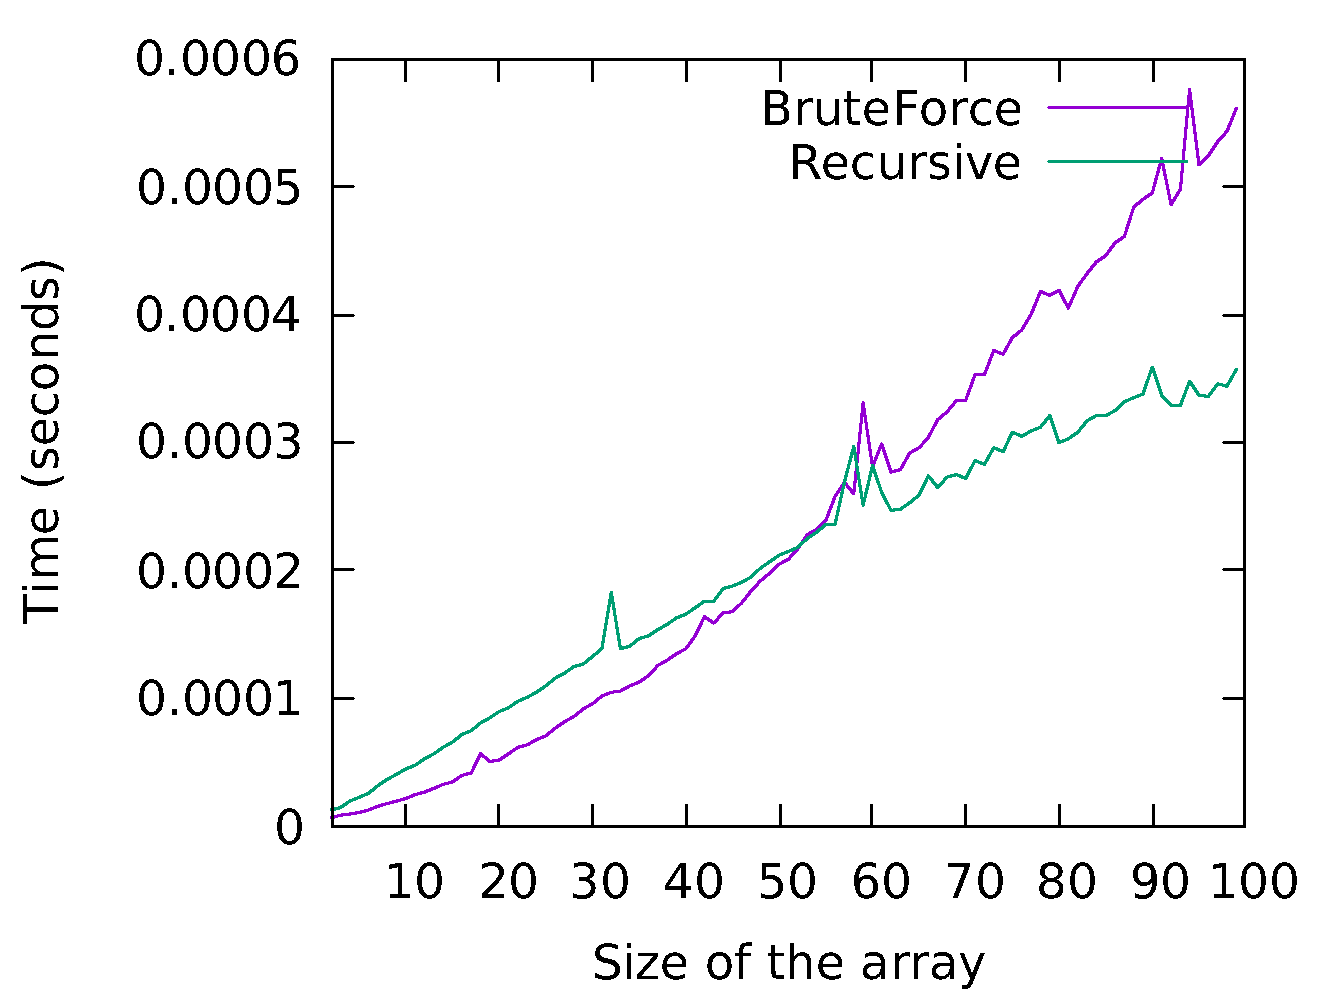
\includegraphics[width=0.35\textwidth]{images/4_1_3_1.pdf}
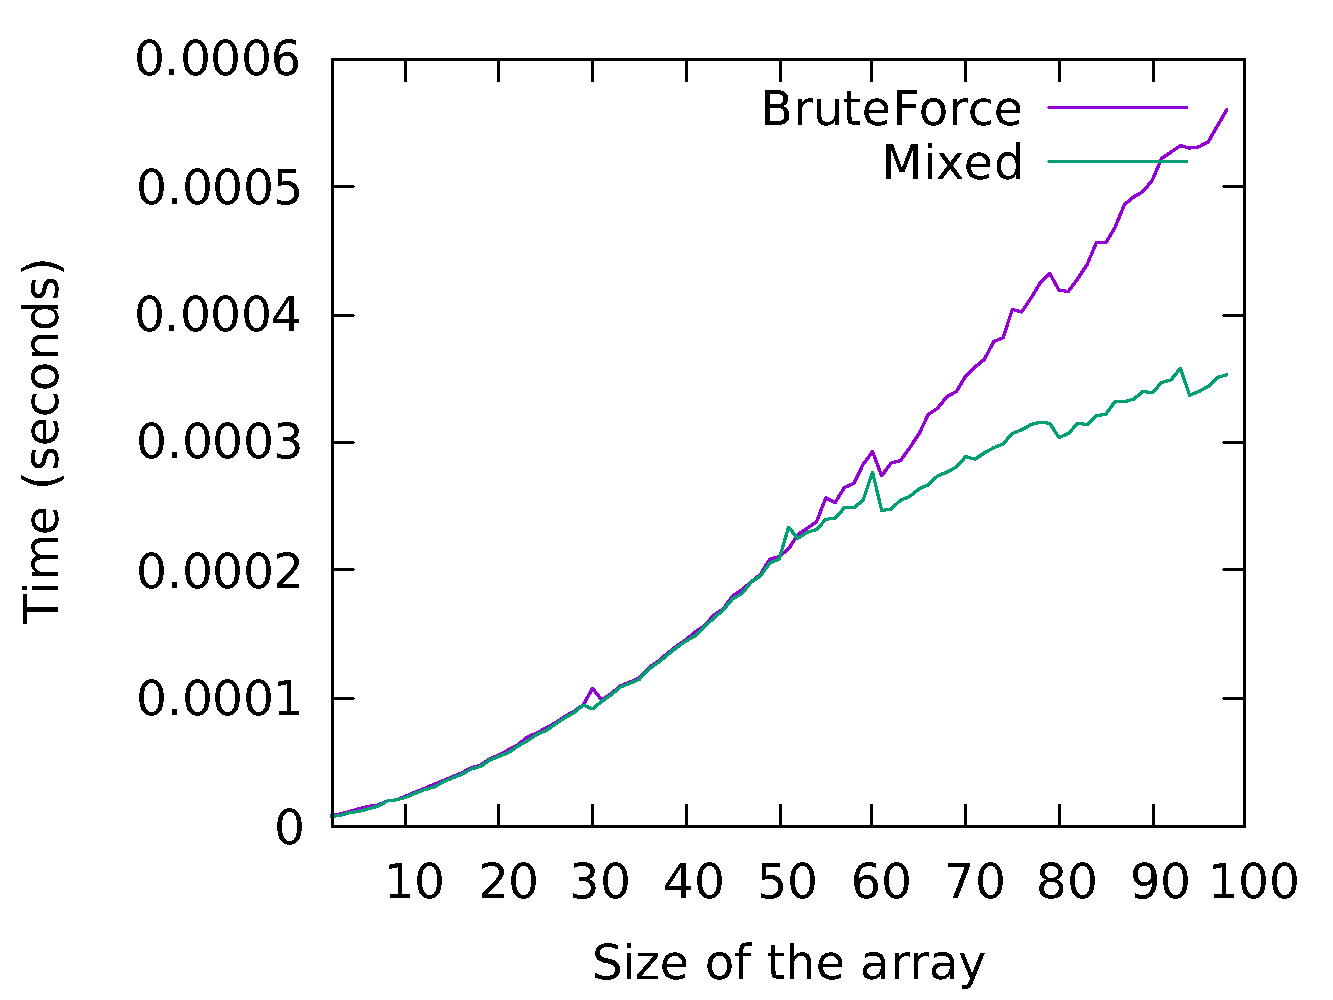
\includegraphics[width=0.35\textwidth]{images/4_1_3_2.pdf}
\end{center}
\end{framed}

\item[4.1{-}4]{Suppose we change the definition of the maximum-subarray problem
to allow the result to be an empty subarray, where the sum of the values of an
empty subarray is 0. How would you change any of the algorithms that do not
allow empty subarrays to permit an empty subarray to be the result?}

\begin{framed}
The BruteForce algorithm (stated above in Question 4.1{-}2) can be updated just
by modifying line 3 to $sum = 0$, instead of $sum = -\infty$. In that case, if
there is no subarray whose sum is greater than zero, the algorithm will return
a invalid subarray ($low = 0, high = 0, sum = 0$), which will denote the empty
subarray.

The Recursive algorithm (stated in Section 4.1) can be updated as follows. In
the \textsc{Find-Max-Crossing-Subarray} routine, update lines 1 and 8 to
initialize $left \mhyphen sum$ and $right \mhyphen sum$ to 0, instead of
$-\infty$. Also initialize $max \mhyphen left$ (after line 1) and $max \mhyphen
right$ (after line 8) to 0. In the \textsc{Find-Maximum-Subarray} routine,
surround the return statement of line 2  with a conditional that
verifies if $A[low]$ is greater than zero. If it is, return the values as it was
before. If it is not, return a invalid subarray (denoted by $low = 0$ and
$high = 0$) and the sum as zero.
\end{framed}

\item[4.1{-}5]{Use the following ideas to develop a nonrecursive, linear-time
algorithm for the maximum-subarray problem. Start at the left end of the
array, and progress toward the right, keeping track of the maximum subarray
seen so far. Knowing a maximum subarray of $A[1, \dots, j]$, extend the answer
to find a maximum subarray ending at index $j + 1$ by using the following
observation: a maximum subarray of $A[1, \dots, j + 1]$ is either a maximum
subarray of $A[1, \dots, j]$ or a subarray $A[i, \dots, j + 1]$, for some
$1 \le i \le j + 1$. Determine a maximum subarray of the form $A[i, \dots,
j + 1]$ in constant time based on knowing a maximum subarray ending at index
$j$.}

\begin{framed}
The pseudocode is stated below.\\
\begin{algorithm}[H]
\SetAlgoNoEnd\DontPrintSemicolon
\BlankLine
\SetKwFunction{algo}{FindMaximumSubarray-Linear}
\SetKwProg{myalg}{}{}{}
\myalg{\algo{A}}{%
\nl $low = 0$\;
\nl $high = 0$\;
\nl $sum = 0$\;
\nl $current \mhyphen low = 0$\;
\nl $current \mhyphen sum = 0$\;
\nl \For{$i = 1$ \KwTo $A.length$}{%
\nl   $current \mhyphen sum = \max(A[i], current \mhyphen sum + A[i])$\;
\nl   \If{$current \mhyphen sum == A[i]$}{%
\nl     $current \mhyphen low = i$\; }
\nl   \If{$current \mhyphen sum > sum$}{%
\nl     $low = current \mhyphen low$\;
\nl     $high = i$\;
\nl     $sum = current \mhyphen sum$\; } }
\nl \Return{$low, high, sum$} }
\end{algorithm}

\vspace{0.5mm}

We can make it a little faster (twice as fast on my machine) by avoiding
executing lines 7, 8, and 10 when not necessary.\\
\begin{algorithm}[H]
\SetAlgoNoEnd\DontPrintSemicolon
\BlankLine
\SetKwFunction{algo}{FindMaximumSubarray-Linear-Optimized}
\SetKwProg{myalg}{}{}{}
\myalg{\algo{A}}{%
\nl $low = 0$\;
\nl $high = 0$\;
\nl $sum = 0$\;
\nl $current \mhyphen low = 0$\;
\nl $current \mhyphen sum = 0$\;
\nl \For{$i = 1$ \KwTo $A.length$}{%
\nl   \If{$current \mhyphen sum + A[i] \le 0$}{%
\nl     $current \mhyphen sum = 0$\; }
\nl   \Else{%
\nl     $current \mhyphen sum = current \mhyphen sum + A[i]$\;
\nl     \If{$current \mhyphen sum == A[i]$}{%
\nl       $current \mhyphen low = i$\; }
\nl     \If{$current \mhyphen sum > sum$}{%
\nl       $low = current \mhyphen low$\;
\nl       $high = i$\;
\nl       $sum = current \mhyphen sum$\; } } }
\nl \Return{$low, high, sum$} }
\end{algorithm}
\end{framed}

\end{enumerate}

\newpage

\section{Strassen's algorithm for matrix multiplication}

\begin{enumerate}

\item[4.2{-}1]{Use Strassen's algorithm to compute the matrix product
\[
\begin{bmatrix}
  1 & 3\\
  7 & 5
\end{bmatrix}
\begin{bmatrix}
  6 & 8\\
  4 & 2
\end{bmatrix}
.
\]
Show your work.
}

\begin{framed}
Let
\[
  A = \begin{bmatrix} 1 & 3\\ 7 & 5 \end{bmatrix},
  B = \begin{bmatrix} 6 & 8\\ 4 & 2 \end{bmatrix},
\]
and $C = A \cdot B$. To compute $C$ using Strassen's algorithm, we start by
computing the $S_i$ matrices:
\begin{equation*}
\begin{aligned}
S_1 \; &= \; B_{12} - B_{22} \; = \; 8 - 2 \; = \; 6,\\
S_2 \; &= \; A_{11} + A_{12} \; = \; 1 + 3 \; = \; 4,\\
S_3 \; &= \; A_{21} + A_{22} \; = \; 7 + 5 \; = \; 12,\\
S_4 \; &= \; B_{21} - B_{11} \; = \; 4 - 6 \; = \; -2,\\
S_5 \; &= \; A_{11} + A_{22} \; = \; 1 + 5 \; = \; 6,\\
S_6 \; &= \; B_{11} + B_{22} \; = \; 6 + 2 \; = \; 8,\\
S_7 \; &= \; A_{12} + A_{22} \; = \; 3 - 5 \; = \; -2,\\
S_8 \; &= \; B_{21} + B_{22} \; = \; 4 + 2 \; = \; 6,\\
S_9 \; &= \; A_{11} - A_{21} \; = \; 1 - 7 \; = \; -6,\\
S_{10} \; &= \; B_{11} + B_{12} \; = \; 6 + 8 \; = \; 14.
\end{aligned}
\end{equation*}

Then we compute the $P_i$ matrices:
\begin{equation*}
\begin{aligned}
  P_1 \; &= \; A_11 \cdot S_1 \; &&= \; 1 \cdot 6 \; &&= \; 6,\\
  P_2 \; &= \; S_2 \cdot B_22 \; &&= \; 4 \cdot 2 \; &&= \; 8,\\
  P_3 \; &= \; S_3 \cdot B_11 \; &&= \; 12 \cdot 6 \; &&= \; 72,\\
  P_4 \; &= \; A_22 \cdot S_4 \; &&= \; 5 \cdot (-2) \; &&= \; -10,\\
  P_5 \; &= \; S_5 \cdot S_6 \; &&= \; 6 \cdot 8 \; &&= \; 48,\\
  P_6 \; &= \; S_7 \cdot S_8 \; &&= \; (-2) \cdot 6 \; &&= \; -12,\\
  P_7 \; &= \; S_9 \cdot S_10 \; &&= \; (-6) \cdot 14 \; &&= \; -84.
\end{aligned}
\end{equation*}

Using matrices $S_i$ and $P_i$, we compute $C$:
\[
C =
\begin{bmatrix}
(P_5 + P_4 - P_2 + P_6) & (P_2 + P_2)\\ (P_3 + P_4) & (P_5 + P_1 - P_3 - P_7)
\end{bmatrix}
=
\begin{bmatrix}
18 & 14\\ 62 & 66
\end{bmatrix}
.
\]
\end{framed}

\newpage

\item[4.2{-}2]{Write pseudocode for Strassen's algorithm.}

\begin{framed}
The pseudocode is stated below.\\
\begin{algorithm}[H]
\SetAlgoNoEnd\DontPrintSemicolon
\BlankLine
\SetKwFunction{algo}{Square-Matrix-Multiply-Strassen}
\SetKwProg{myalg}{}{}{}
\myalg{\algo{A, B}}{%
\nl $n = A.rows$\;
\nl let $C$ be a new $n \times n$ matrix\;
\nl \If{$n == 1$}{%
\nl   $c_{11} = a_{11} \cdot b_{11}$\; }
\nl \Else{%
\nl   partition $A, B$, and $C$ as into $n/2 \times n/2$ submatrices\;
\nl   let $S_1, S_2, \dots, S_{10}$ be new $n/2 \times n/2$ matrices\;
\nl   let $P_1, P_2, \dots, P_7$ be new $n/2 \times n/2$ matrices\;
\nl   $S_1 = B_{12} - B_{22}$\;
\nl   $S_2 = A_{11} + A_{12}$\;
\nl   $S_3 = A_{21} + A_{22}$\;
\nl   $S_4 = B_{21} - B_{11}$\;
\nl   $S_5 = A_{11} + A_{22}$\;
\nl   $S_6 = B_{11} + B_{22}$\;
\nl   $S_7 = A_{12} - A_{22}$\;
\nl   $S_8 = B_{21} + B_{22}$\;
\nl   $S_9 = A_{11} - A_{21}$\;
\nl   $S_{10} = B_{11} - B_{12}$\;
\nl   $P_1 =$ \texttt{Square-Matrix-Multiply-Strassen}($A_{11}, S_1$)\;
\nl   $P_2 =$ \texttt{Square-Matrix-Multiply-Strassen}($S_2, B_{22}$)\;
\nl   $P_3 =$ \texttt{Square-Matrix-Multiply-Strassen}($S_3, B_{11}$)\;
\nl   $P_4 =$ \texttt{Square-Matrix-Multiply-Strassen}($A_{22}, S_4$)\;
\nl   $P_5 =$ \texttt{Square-Matrix-Multiply-Strassen}($S_5, S_6$)\;
\nl   $P_6 =$ \texttt{Square-Matrix-Multiply-Strassen}($S_7, S_8$)\;
\nl   $P_7 =$ \texttt{Square-Matrix-Multiply-Strassen}($S_9, S_{10}$)\;
\nl   $C_{11} = P_5 + P_4 - P_2 + P_6$ \;
\nl   $C_{12} = P_1 + P_2$ \;
\nl   $C_{21} = P_3 + P_4$ \;
\nl   $C_{22} = P_5 + P_1 - P_3 - P_7$ \; }
\nl \Return{$C$} }
\end{algorithm}
\end{framed}

\item[4.2{-}3]{How would you modify Strassen's algorithm to multiply $n \times
n$ matrices in which $n$ is not an exact power of 2? Show that the resulting
algorithm runs in time $\Theta(n^{\lg 7})$.}

\begin{framed}
Pad each input $n \times n$ matrix (rows and columns) with $m - n$ zeros,
resulting in an $m \times m$ matrix, where $m = 2^{\ceil{\lg n}}$. After
computing the final matrix, cut down the last $m - n$ rows and $m - n$ columns
(which will be zeros).

Padding the matrix with zeros is done once, in the root of the recursion tree,
and takes $O(m^2)$. Since we now have an $m \times m$ matrix, the algorithm runs
in $\Theta(m^{\lg 7}) + O(m^2) = \Theta(m^{\lg 7})$. We have that
$n \le m <  2^{(\lg n) + 1} = 2^{\lg n} \cdot 2 = 2n.$ Thus, the
algorithm runs in $\Theta((2n)^{\lg 7}) = \Theta(n^{\lg 7})$.
\end{framed}

\item[4.2{-}4]{What is the largest $k$ such that if you can multiply
$3 \times 3$ matrices using $k$ multiplications (not assuming commutativity of
multiplication), then you can multiply $n \times n$ matrices in time
$o(n^{\lg 7})$?  What would the running time of this algorithm be?
}

\begin{framed}
If we modify the \textsc{Square-Matrix-Multiply-Recursive} algorithm to
partition the matrices into $n/3 \times n/3$ submatrices, we would have the
following recurrence:
\[
T(n) = \Theta(1) + 27 T(n/3) + \Theta(n^2) = 27 T(n/3) + \Theta(n^2).
\]

Let's proceed to understand a little more about the above recurrence. Let $A$
and $B$ be the two input matrices in each node of the above recursion tree.
Like in the original \textsc{Square-Matrix-Multiply-Recursive} algorithm, our
modified version will take $\Theta(1)$ to partition $A$ and $B$ into $n/3 \times
n/3$ submatrices. In each node of the tree, the product of $A$ and $B$ is
recursively computed by the products of their submatrices. Since the number of
recursive (submatrices) products to compute $A \cdot B$ in each node of the
recurstion tree is 27 and each of these submatrices is $3$ times smaller than
$A$ and $B$, the 27 recursive products takes $27 T(n/3)$. Finally, the number of
summations to compute the final matrix is
$\Theta(3 \cdot 9 \cdot n^2/3) = \Theta(n^2)$.

If after partitioning $A$ and $B$ into $n/3 \times n/3$ submatrices we can
compute their product with $k$ multiplications (instead of 27), we would have
the following recurrence:
\[
T(n) = \Theta(1) + k T(n/3) + \Theta(n^2) = k T(n/3) + \Theta(n^2),
\]

We can solve the above recurrence using the master method. We have
$f(n) = n^2$ and $n^{log_b a} = n^{\log_3 k}$. Using the first case of the master
method, we have
\[
\Forall k \; | \log_3 k > 2, \; n^2 = O(n^{(\log_3 k) - \epsilon}), \; 0 \le \epsilon \le \log_3 k - 2,
\]
which implies
\[
T(n) = \Theta(n^{\log_3 k}).
\]

Since $\log_3 21 < \lg 7 < \log_3 22$, the largest value for $k$ is 21. Its
running time would be $n^{\log_3 21} \approx n^{2.7712}$.

\end{framed}

\item[4.2{-}5]{V. Pan has discovered a way of multiplying $68 \times 68$
matrices using 132,464 multiplications, a way of multiplying $70 \times 70$
matrices using 143,640 multiplications, and a way of multiplying $72 \times 72$
matrices using 155,424 multiplications. Which method yields the best asymptotic
running time when used in a divide-and-conquer matrix-multiplication algorithm?
How does it compare to Strassen's algorithm?}

\begin{framed}
The algorithms would take:
\begin{itemize}
  \item $n^{\log_{68} 132,464} \approx n^{2.795128}$,
  \item $n^{\log_{70} 143,640} \approx n^{2.795122}$,
  \item $n^{\log_{72} 155,424} \approx n^{2.795147}$.
\end{itemize}

The fastest is the one that multiplies $70 \times 70$ matrices, but all of them
are faster then the Strassen's algorithm.
\end{framed}

\item[4.2{-}6]{How quickly can you multiply a $k n \times n$ matrix by an
$n \times k n$ matrix, using Strassen's algorithm as a subroutine? Answer the
same question with the order of the input matrices reversed.}

\begin{framed}
Let $A$ and $B$ be $kn \times n$ and $n \times k n$ matrices, respectivelly. We
can compute $A \cdot B$ as follows:
\begin{enumerate}
\item Partition $A$ and $B$ into $k$ submatrices $A_1, \dots, A_k$ and $B_1,
\dots, B_k$, each one of size $n \times n$.
\item Compute the desired submatrices $C_{ij}$ of the result matrix $C$ by the
product of $A_i \cdot B_j$. Use the Strassen's algorithm to compute each of
those products.
\end{enumerate}

Since each of the $k^2$ products takes $\Theta(n^{\lg 7})$, this algorithm
runs in $\Theta(k^2 n^{\lg 7})$.

We can compute $B \cdot A$ as follows:
\begin{enumerate}
\item Partition $A$ and $B$ into $k$ submatrices $A_1, \dots, A_k$ and $B_1,
\dots, B_k$, each one of size $n \times n$.
\item Compute the the result matrix $C = \sum_{i = 1}^{k} A_i \cdot B_i$.
Use the Strassen's algorithm to compute each of those products.
\end{enumerate}

Since each of the $k$ products takes $\Theta(n^{\lg 7})$ and the $k - 1$
summations takes $\Theta((k - 1) {n^2}/k) = O(n^2)$, this algorithm runs in
$\Theta(k n^{\lg 7}) + O(n^2) = \Theta(k n^{\lg 7})$.

\end{framed}

\item[4.2{-}7]{Show how to multiply the complex numbers $a + b i$ and $c + di$
using only three multiplications of real numbers. The algorithm should take
$a, b, c$, and $d$ as input and produce the real component $ac - bd$ and the
imaginary component $ad + bc$ separately.}

\begin{framed}
The pseudocode is stated below.\\
\begin{algorithm}[H]
\SetAlgoNoEnd\DontPrintSemicolon
\BlankLine
\SetKwFunction{algo}{Complex-Product}
\SetKwProg{myalg}{}{}{}
\myalg{\algo{a, b, c, d}}{%
\nl $x = a \cdot c$\;
\nl $y = b \cdot d$\;
\nl $real \mhyphen part = x - y$\;
\nl $imaginary \mhyphen part = (a + b) \cdot (c + d) - x - y$\;
\nl \Return{$real \mhyphen part, imaginary \mhyphen part$} }
\end{algorithm}
\end{framed}

\end{enumerate}

\newpage

\section{The substitution method for solving recurrences}

\begin{enumerate}

\item[4.3{-}1]{Show that the solution of $T(n) = T(n - 1) + n$ is $O(n^2)$.}

\begin{framed}
Our guess is
\[
T(n) \le cn^2 \; \Forall n \ge n_0,
\]
where $c$ and $n_0$ are positive constants. Substituting into the recurrence
yields
\begin{equation*}
\begin{aligned}
T(n) &\le c (n - 1)^2 + n\\
     &= cn^2 - 2cn + c + n & \text{($c = 1$)}\\
     &= n^2 - 2n + n + 1\\
     &= n^2 - n + 1\\
     &\le n^2,
\end{aligned}
\end{equation*}
where the last step holds as long as $n_0 \ge 1$.

\end{framed}

\item[4.3{-}2]{Show that the solution of $T(n) = T(\ceil{n/2}) + 1$ is
$O(\lg n)$.}

\begin{framed}
Our guess is
\[
T(n) \le c \lg n - d \; \Forall n \ge n_0,
\]
where $c$, $d$, and $n_0$ are positive constants. Substituting into the
recurrence yields
\begin{equation*}
\begin{aligned}
T(n) &\le c \lg(\ceil{n/2}) - d + 1\\
     &\le c \lg n - d + 1\\
     &\le c \lg n,
\end{aligned}
\end{equation*}
where the last step holds as long as $d \ge 1$.
\end{framed}

\item[4.3{-}3]{We saw that the solution of $T(n) = 2T(\floor{n/2}) + n$ is
$O(n \lg n)$. Show that the solution of this recurrence is also
$\Omega(n \lg n)$. Conclude that the solution is $\Theta(n \lg n)$.}

\begin{framed}
Our guess is
\[
T(n) \ge c n \lg n \; \Forall n \ge n_0,
\]
where $c$ and $n_0$ are positive constants. Substituting into the
recurrence yields
\begin{equation*}
\begin{aligned}
T(n) &\ge 2(c \floor{n/2} \lg\floor{n/2}) + n\\
     &\ge 2 c (n/4) \lg(n/4) + n\\
     &=   c (n/2) \lg n - c (n/2) \lg 4 + n\\
     &=   c (n/2) \lg n - c n + n\\
     &\ge c n \lg n,
\end{aligned}
\end{equation*}
where the last step holds as long as $c \le 1$.

Thus, we have
\[
c_1 n \lg n \le T(n) \le c_2 n \lg n,
\]
with $c_1 \le 1$ and $c_2 \ge 1$, which implies
\[
T(n) = \Theta(n \lg n).
\]
\end{framed}

\newpage

\item[4.3{-}4]{Show that by making a different inductive hypothesis, we can
overcome the difficulty with the boundary condition $T(1) = 1$ for recurrence
(4.19) without adjusting the boundary conditions for the inductive proof.}

\begin{framed}
Our new guess is
\[
T(n) \le c n \lg n + n \; \Forall n \ge n_0,
\]
where $c$, $d$, and $n_0$ are positive constants. Substituting into the
recurrence yields
\begin{equation*}
\begin{aligned}
T(n) &\le 2(c \floor{n/2} \lg \floor{n/2} + \floor{n/2}) + n\\
     &\le cn \lg (n/2) + 2(n/2) + n\\
     &= cn \lg n - cn \lg 2 n + 2n\\
     &= cn \lg n - cn + 2n\\
     &\le c n \lg n + n,
\end{aligned}
\end{equation*}
where the last step holds as long as $c \ge 1$.

Now on the boundary condition, we have
\[
T(1) \le c (n \lg n) + n = c 1 \lg 1 + 1 = 0 + 1 = 1.
\]
\end{framed}

\item[4.3{-}5]{Show that $\Theta(n \lg n)$ is the solution to the ``exact''
recurrence (4.3) for merge sort.}

\begin{framed}
First, we verify if (4.3) is $O(n \lg n)$. Our guess is
\[
T(n) \le c (n - d) \lg (n - d) \; \Forall n \ge n_0,
\]
where $c$, $d$, and $n_0$ are positive constants. Substituting into the
recurrence yields
\begin{equation*}
\begin{aligned}
T(n) &\le c (\ceil{n/2} - d) \lg (\ceil{n/2} - d) + c (\floor{n/2} - d) \lg (\floor{n/2} - d) + en\\
     &\le c (n/2 + 1 - d) \lg (n/2 + 1 - d) + c (n/2 - d) \lg (n/2 - d) + en & \text{($d \ge 2$)}\\
     &\le c\left(\frac{n - d}{2}\right) \lg \left(\frac{n - d}{2}\right)
     + c\left(\frac{n - d}{2}\right) \lg\left(\frac{n - d}{2}\right) + en\\
     &= c (n - d) \lg \left(\frac{n - d}{2}\right) + en\\
     &= c (n - d) \lg (n - d) - c (n - d) + en\\
     &= c (n - d) \lg (n - d) - cn + en + cd\\
     &\le c (n - d) \lg (n - d),
\end{aligned}
\end{equation*}
where the last step holds as long as $c > e$ and $n_0 \ge cd$.

Then we verify if (4.3) is $\Omega(n \lg n)$. Our guess is
\[
T(n) \ge c (n + d) \lg (n + d) \; \Forall n \ge n_0,
\]
where $c$, $d$, and $n_0$ are positive constants. Substituting into the
recurrence yields
\begin{equation*}
\begin{aligned}
T(n) &\ge c (\ceil{n/2} + d) \lg (\ceil{n/2} + d) + c (\floor{n/2} + d) \lg (\floor{n/2} + d) + en\\
     &\ge c (n/2 + d) \lg (n/2 + d) + c (n/2 - 1 + d) \lg (n/2 - 1 + d) + en & \text{($d \ge 2$)}\\
     &\ge c\left(\frac{n + d}{2}\right) \lg \left(\frac{n + d}{2}\right)
     + c\left(\frac{n + d}{2}\right) \lg\left(\frac{n + d}{2}\right) + en\\
     &= c (n + d) \lg \left(\frac{n + d}{2}\right) + en\\
     &= c (n + d) \lg (n + d) - c (n + d) + en\\
     &= c (n + d) \lg (n + d) - cn + en - cd\\
     &\ge c (n + d) \lg (n + d),
\end{aligned}
\end{equation*}
where the last step holds as long as $e > c$ and $n_0 \ge cd$.
\end{framed}

\newpage

\item[4.3{-}6]{Show that the solution to $T(n) = 2T(\floor{n/2} + 17) + n$ is
$O(n \lg n)$.}

\begin{framed}
Our guess is
\[
T(n) \le c (n - d) \lg (n - d) \; \Forall n \ge n_0,
\]
where $c$, $d$, and $n_0$ are positive constants. Substituting into the
recurrence yields
\begin{equation*}
\begin{aligned}
T(n) &\le 2 c (\floor{n/2} - d + 17) \lg (\floor{n/2} - d + 17) + n\\
     &\le 2 c (n/2 - d + 17) \lg (n/2 - d + 17) + n & \text{($d \ge 34$)}\\
     &\le 2 c\left(\frac{n - d}{2}\right) \lg \left(\frac{n - d}{2}\right) + n\\
     &= c (n - d) \lg \left(\frac{n - d}{2}\right) + n\\
     &= c (n - d) \lg (n - d) - c (n - d) + n\\
     &= c (n - d) \lg (n - d) - cn + n + cd\\
     &\le c (n - d) \lg (n - d),
\end{aligned}
\end{equation*}
where the last step holds as long as $c \ge 2$ and $n_0 \ge cd$.
\end{framed}

\item[4.3{-}7]{Using the master method in Section 4.5 you can show that the
solution to the recurrence $T(n) = 4T(n/3) + n$ is
$T(n) = \Theta(n^{\log_3 4})$. Show that a substitution proof with the
assumption $T(n) \le c n^{\log_3 4}$ fails. Then show how to subtract off a
lower-order term to make a substitution proof work.}

\begin{framed}
The initial guess is
\[
T(n) \le c n^{\log_3 4} \; \Forall n \ge n_0,
\]
where $c$, and $n_0$ are positive constants. Substituting into the
recurrence yields
\begin{equation*}
\begin{aligned}
T(n) &\le 4 c \left(\frac{n}{3}\right)^{\log_3 4} + n\\
     &= 4 c \frac{n^{\log_3 4}}{4} + n\\
     &= c n^{\log_3 4} + n
\end{aligned}
\end{equation*}
which does not imply $T(n) \le c n^{\log_3 4}$ for any choice of $c$.

Our new guess is
\[
T(n) \le c n^{\log_3 4} - dn \; \Forall n \ge n_0,
\]
where $c$, $d$, and $n_0$ are positive constants. Substituting into the
recurrence yields
\begin{equation*}
\begin{aligned}
T(n) &\le 4 \left(c \left(\frac{n}{3}\right)^{\log_3 4} - d \frac{n}{3}\right) + n\\
     &= 4 c \frac{n^{\log_3 4}}{4} - 4d \frac{n}{3} + n\\
     &\le c n^{\log_3 4},
\end{aligned}
\end{equation*}
where the last step holds as long as $d \ge 3/4$.
\end{framed}

\item[4.3{-}8]{Using the master method in Section 4.5, you can show that the
solution to the recurrence $T(n) = 4T(n/2) + n$ is $T(n) = \Theta(n^2)$. Show
that a substitution proof with the assumption $T(n) \le cn^2$ fails. Then show
how to subtract off a lower-order term to make a substitution proof work.}

\begin{framed}
The initial guess is
\[
T(n) \le c n^2 \; \Forall n \ge n_0,
\]
where $c$, and $n_0$ are positive constants. Substituting into the
recurrence yields
\begin{equation*}
\begin{aligned}
T(n) &\le 4 c \left(\frac{n}{2}\right)^2 + n\\
     &= c n^2 + n
\end{aligned}
\end{equation*}
which does not imply $T(n) \le c n^2$ for any choice of $c$.

Our new guess is
\[
T(n) \le c n^2 - dn \; \Forall n \ge n_0,
\]
where $c$, $d$, and $n_0$ are positive constants. Substituting into the
recurrence yields
\begin{equation*}
\begin{aligned}
T(n) &\le 4 \left(c \left(\frac{n}{2}\right)^2 - d\frac{n}{2} \right) + n\\
     &= c n^2 - 2dn + n\\
     &\le c n^2,
\end{aligned}
\end{equation*}
where the last step holds as long as $d \ge 1/2$.
\end{framed}

\item[4.3{-}9]{Solve the recurrence $T(n) = 3T(\sqrt{n}) + \log n$ by making
a change of variables.  Your solution should be asymptotically tight. Do not
worry about whether values are integral.}

\begin{framed}
Renaming $m = \log n$ yields
\[
T(10^m) = 3T(10^{m/2}) + m.
\]

Now renaming $S(m) = T(2^m)$ yields
\[
S(m) = 3S(m/2) + m.
\]

With the master method, we have $f(n) = m = \log n$ and
$n^{\log_b a} = n^{\lg 3} \approx n^{1.585}$. Using the first case, we have
\[
f(n) = \log n = O(n^{\lg 3 - \epsilon}), \; \text{($\epsilon = 0.5$)}
\]
which implies
\[
S(m) = \Theta(m^{\lg 3}).
\]

We can double-check if $S(m) = O(m^{\lg 3})$ using the substition method. Our
guess is
\[
S(m) \le c m^{\lg 3} - dm \; \Forall m \ge m_0,
\]
where $c$, $d$, and $n_0$ are positive constants. Substituting into the
recurrence yields
\begin{equation*}
\begin{aligned}
T(n) &\le 3 \left(c \left(\frac{m}{2}\right)^{\lg 3} - d \frac{m}{2}\right) + m\\
     &= 3 c \frac{m^{\lg 3}}{3} - 3d\frac{m}{2} + m\\
     &\le c m^{\lg 3} + dm
\end{aligned}
\end{equation*}
where the last step holds as long as $d \ge 2/3$.

Now verifying if $S(m) = \Omega(m^{\lg 3})$ with the substitution method. Our
guess is
\[
S(m) \ge c m^{\lg 3} \; \Forall m \ge m_0,
\]
where $c$, and $n_0$ are positive constants. Substituting into the
recurrence yields
\begin{equation*}
\begin{aligned}
T(n) &\ge 3 c \left(\frac{m}{2}\right)^{\lg 3} + m\\
     &= 3 c \frac{m^{\lg 3}}{3} + m\\
     &\ge c m^{\lg 3}.
\end{aligned}
\end{equation*}

Finally, we have
\[
T(n) = T(10^m) = S(m) = \Theta(m^{\lg 3}) = \Theta(\log^{\lg 3} n).
\]

\end{framed}

\end{enumerate}

\newpage

\section{The recursion-tree method for solving recurrences}

\begin{enumerate}

\item[4.4{-}1]{Use a recursion tree to determine a good asymptotic upper bound
on the recurrence $T(n) = 3T(\floor{n/2}) + n$. Use the substitution method to
verify your answer.}

\begin{framed}
Since floors/ceiling usually do not matter, we will draw a recursion tree for
the recurrence $T(n) = 3T(n/2) + n$.

\begin{center}
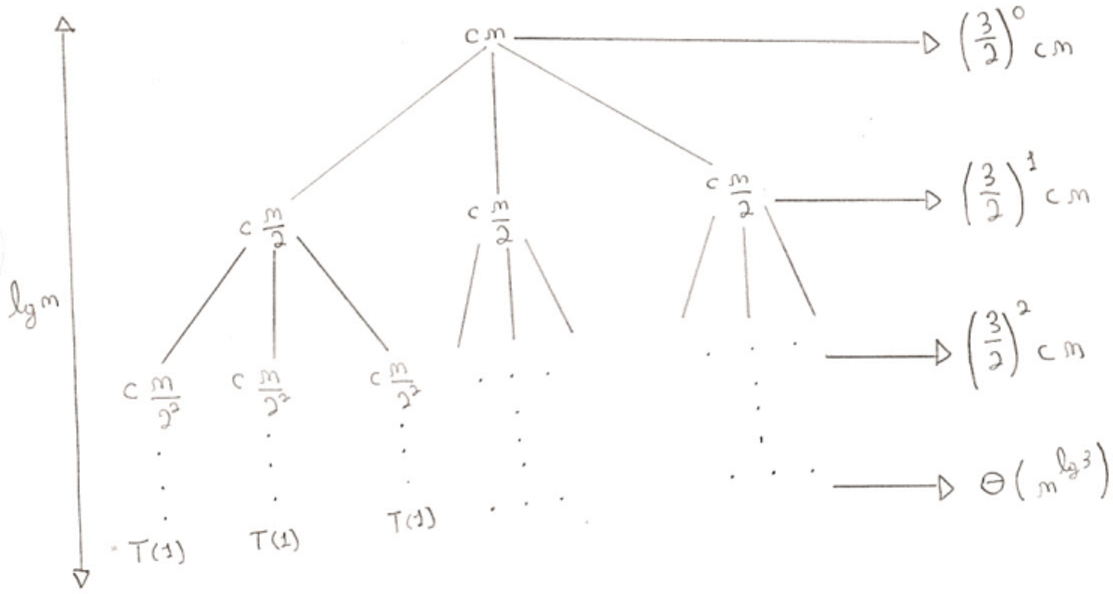
\includegraphics[width=0.7\textwidth]{images/4_4_1_1.pdf}
\end{center}

The number of nodes at depth $i$ is $3^i$. Since subproblem size reduce by
a factor of 2, each node at depth $i$, for $i = 0, 1, 2, \dots, \lg n - 1$,
has a cost of $c (n/2^i)$. Thus, the total cost over all nodes at depth
$i$, for $i = 0, 1, 2, \dots, \lg n - 1$, is $(3/2)^i cn$. The bottom level,
at deph $\lg n$, has $3^{\lg n} = n^{\lg 3}$ nodes, each contributing cost
$T(1)$, for a total cost of $n^{\lg 3} T(1) = \Theta(n^{\lg 3})$.

The cost of the entire tree is
\begin{equation*}
\begin{aligned}
T(n) &= cn + \frac{3}{2} cn + \left(\frac{3}{2}\right)^2 cn + \dots
           + \left(\frac{3}{2}\right)^{\lg n - 1} cn + \Theta\left({n^{\lg 3}}\right)\\
     &= \sum_{i = 0}^{\lg n - 1} \left(\frac{3}{2}\right)^i cn + \Theta(n^{\lg 3})\\
     &= cn \frac{\left(\frac{3}{2}\right)^{\lg n} - 1}{\frac{3}{2} - 1} + \Theta(n^{\lg 3})\\
     &= 2cn \left(\left(\frac{3}{2}\right)^{\lg n} - 1\right) + \Theta(n^{\lg 3})\\
     &= 2cn \frac{3^{\lg n}}{2^{\lg n}} - 2cn + \Theta(n^{\lg 3})\\
     &= 2cn \frac{n^{\lg 3}}{n} - 2cn + \Theta(n^{\lg 3})\\
     &= 2cn^{\lg 3} - 2cn + \Theta(n^{\lg 3})\\
     &= O(n^{\lg 3}).
\end{aligned}
\end{equation*}

Our guess is
\[
T(n) \le c n^{\lg 3} - dn \; \Forall n \ge n_0,
\]
where $c$, $d$, and $n_0$ are positive constants. Substituting into the
recurrence yields
\begin{equation*}
\begin{aligned}
  T(n) &\le 3 \left(c {\Bigl\lfloor\frac{n}{2}\Bigl\rfloor}^{\lg 3} - d {\Bigl\lfloor\frac{n}{2}\Bigl\rfloor}\right) + n\\
       &\le \frac{3c}{3} n^{\lg 3} - \frac{3d}{2}n + n\\
       &= c n^{\lg 3} - dn - \frac{d}{2}n + n\\
       &\le c n^{\lg 3} - dn,
\end{aligned}
\end{equation*}
where the last step holds as long as $d \ge 2$.
\end{framed}

\newpage

\item[4.4{-}2]{Use a recursion tree to determine a good asymptotic upper bound
on the recurrence $T(n) = T(n/2) + n^2$. Use the substitution method to verify
your answer.}

\begin{framed}
Figure below ilustrates the recursion tree $T(n) = T(n/2) + n^2$.

\begin{center}
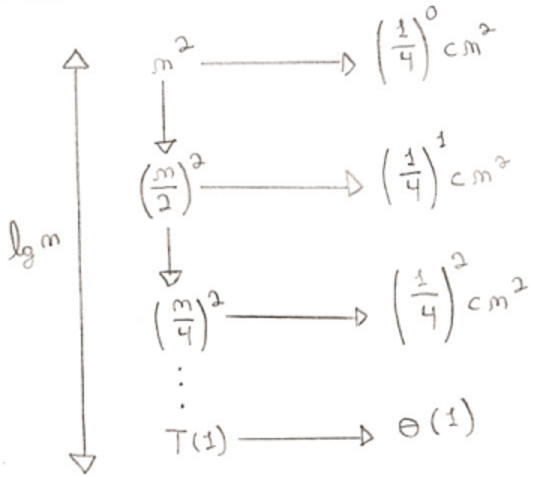
\includegraphics[width=0.3\textwidth]{images/4_4_2_1.pdf}
\end{center}

The tree has $\lg n$ levels and the cost at depth $i$ is
$c(n/2^i)^2 = (1/4)^i cn^2$.

The cost of the entire tree is
\begin{equation*}
\begin{aligned}
T(n) &= \sum_{i = 0}^{\lg n} \left(\frac{1}{4}\right)^i cn^2\\
     &< \sum_{i = 0}^{\infty} \left(\frac{1}{4}\right)^i cn^2\\
     &= \frac{1}{1 - (1/4)} cn^2\\
     &= \frac{4}{3} cn^2\\
     &= O(n^2).
\end{aligned}
\end{equation*}

Our guess is
\[
T(n) \le d n^2 \; \Forall n \ge n_0,
\]
where $d$, and $n_0$ are positive constants. Substituting into the
recurrence and using the same constant $c > 0$ as before yields
\begin{equation*}
\begin{aligned}
  T(n) &\le d \left(\frac{n}{2}\right)^2 + c n^2\\
       &= \frac{1}{4} dn^2 + cn^2\\
       &\le dn^2,
\end{aligned}
\end{equation*}
where the last step holds as long as $d \ge (4/3)c$.
\end{framed}

\newpage

\item[4.4{-}3]{Use a recursion tree to determine a good asymptotic upper bound
on the recurrence $T(n) = 4T(n/2 + 2) + n$. Use the substitution method to
verify your answer.}

\begin{framed}
Figure below ilustrates the recursion tree $T(n) = 4T(n/2 + 2) + n$.

\begin{center}
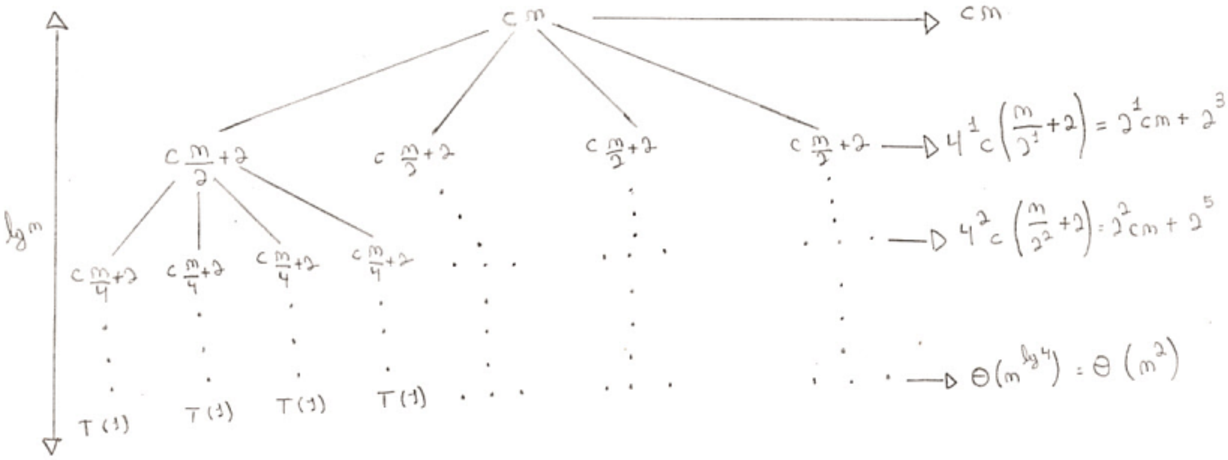
\includegraphics[width=0.9\textwidth]{images/4_4_3_1.pdf}
\end{center}

The number of nodes at depth $i$ is $4^i$. Since subproblem size reduce by
a factor of 2 and increment 2, each node at depth $i$, for
$i = 0, 1, 2, \dots, \lg n - 1$, has a cost of $c (n/2^i + 2)$. Thus, the total
cost over all nodes at depth $i$, for $i = 0, 1, 2, \dots, \lg n - 1$, is
$4^i c (n/2^i + 2) = 2^i cn + 2^{2i + 1}$. The bottom level, at deph $\lg n$,
has $4^{\lg n} = n^{\lg 4}$ nodes, each contributing cost $T(1)$, for a total
cost of $n^{\lg 4} T(1) = \Theta(n^{\lg 4})$.

The cost of the entire tree is
\begin{equation*}
\begin{aligned}
T(n) &= \sum_{i = 0}^{\lg n - 1} \left(4^i c \left(\frac{n}{2^i} + 2\right)\right) +
        \Theta(n^2)\\
     &= \sum_{i = 0}^{\lg n - 1} \left(4^i c \cdot \frac{n}{2^i}\right) +
        \sum_{i = 0}^{\lg n - 1} (4^i c \cdot 2) + \Theta(n^2)\\
     &= cn \sum_{i = 0}^{\lg n - 1} (2^i) + 2c \sum_{i = 0}^{\lg n - 1} (4^i) + \Theta(n^2)\\
     &= cn \frac{2^{\lg n} - 1}{2 - 1} + 2c \frac{4^{\lg n} - 1}{4 - 1} + \Theta(n^2)\\
     &= cn (n - 1) + \frac{2c}{3} (n^2 - 1) + \Theta(n^2)\\
     &= cn^2 - cn + \frac{2cn^2}{3} - \frac{2c}{3} + \Theta(n^2)\\
     &= O(n^2).
\end{aligned}
\end{equation*}

Our guess is
\[
T(n) \le c n^2 - dn \; \Forall n \ge n_0,
\]
where $c$, $d$, and $n_0$ are positive constants. Substituting into the
recurrence yields
\begin{equation*}
\begin{aligned}
  T(n) &\le 4 \left(c \left(\frac{n}{2} + 2\right)^2 - d\left(\frac{n}{2} + 2\right)\right) + n\\
       &\le 4 \left(c \frac{n^2}{4} + 2cn + 4c - \frac{dn}{2} - 2d\right) + n\\
       &= c n^2 + 8cn + 16c - 2dn - 8d + n\\
       &= c n^2 - dn - (d - 8c - 1)n - (d - 2c)8\\
       &\le c n^2 - dn,
\end{aligned}
\end{equation*}
where the last step holds as long as $d - 8c - 1 \ge 0$.
\end{framed}

\newpage

\item[4.4{-}4]{Use a recursion tree to determine a good asymptotic upper bound
on the recurrence $T(n) = 2T(n - 1) + 1$. Use the substitution method to verify
your answer.}

\begin{framed}
Figure below ilustrates the recursion tree $T(n) = 2T(n - 1) + 1$.

\begin{center}
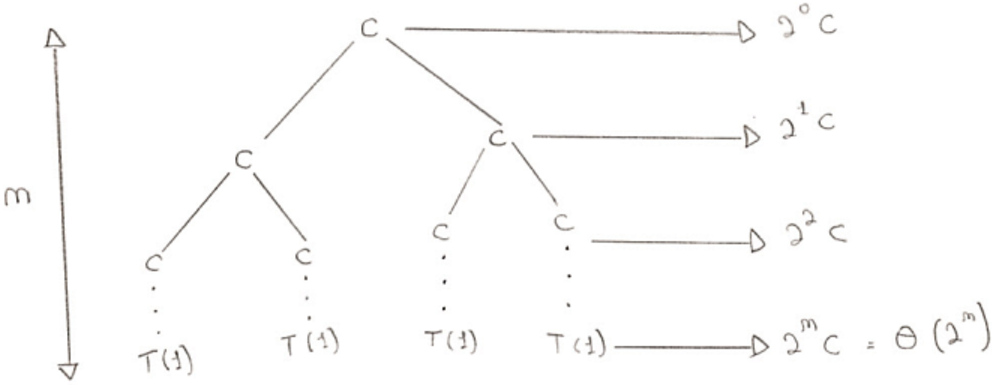
\includegraphics[width=0.6\textwidth]{images/4_4_4_1.pdf}
\end{center}

The tree has $n$ levels and $2^i$ nodes at each level. Since each node costs
$1$, the cost at depth $i$ is $2^i$. The bottom level, at deph $n$,
has $2^n$ nodes, each contributing cost $1$, for a total
cost of $2^n = \Theta(2^n)$.

The cost of the entire tree is
\begin{equation*}
\begin{aligned}
  T(n) &= \sum_{i = 0}^{n - 1} (2^i) + \Theta(2^n)\\
       &= \frac{2^n - 1}{2 - 1} + \Theta(2^n)\\
       &= 2^n - 1 + \Theta(2^n)\\
       &= O(2^n).
\end{aligned}
\end{equation*}

Our guess is
\[
T(n) \le c 2^n - d \; \Forall n \ge n_0,
\]
where $c$, $d$, and $n_0$ are positive constants. Substituting into the
recurrence yields
\begin{equation*}
\begin{aligned}
  T(n) &\le 2 (c 2^{n - 1} - d) + 1\\
       &= c2^n - 2d + 1\\
       &= c2^n - d - d + 1\\
       &\le c 2^n - d,
\end{aligned}
\end{equation*}
where the last step holds as long as $d \ge 1$.
\end{framed}

\newpage

\item[4.4{-}5]{Use a recursion tree to determine a good asymptotic upper bound
on the recurrence $T(n) = T(n - 1) + T(n/2) + n$. Use the substitution method to
verify your answer.}

\begin{framed}
Figure below ilustrates the recursion tree $T(n) = T(n - 1) + T(n/2) + n$.

\begin{center}
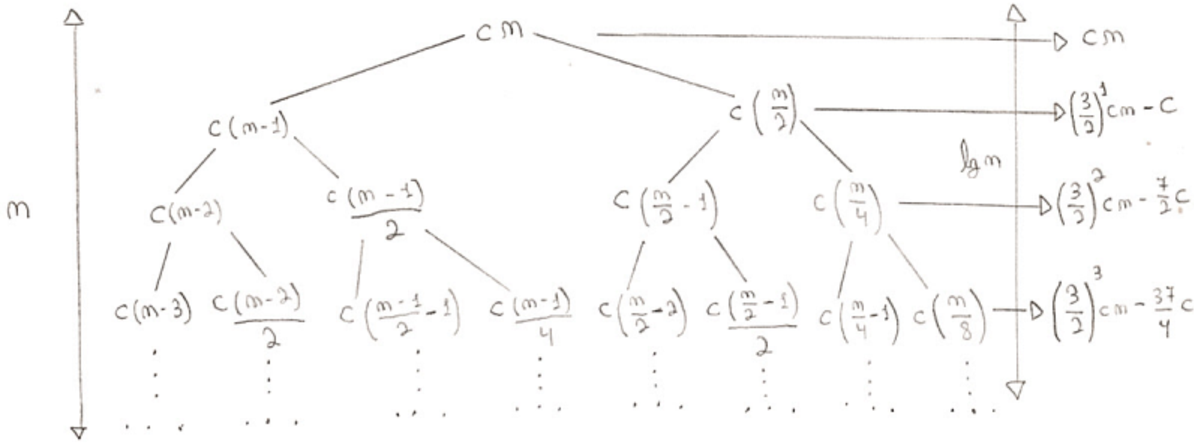
\includegraphics[width=0.85\textwidth]{images/4_4_5_1.pdf}
\end{center}

We start obtaining a lower bound. The cost of the initial levels (before level
$\lg n$) of the tree are
\[
cn \rightarrow (3/2)^1 cn - c \rightarrow (3/2)^2 cn - (7/2) c \rightarrow (3/2)^3 cn - (37/4) c.
\]

Thus, the cost of the tree from the root to level $\lg n$ is at most
\[
  \sum_{i = 0}^{\lg n} \left(\frac{3}{2}\right)^i cn
  = cn \frac{\left(\frac{3}{2}\right)^{\lg n + 1} - 1}{\frac{3}{2} - 1}
  = 2cn \frac{3}{2} \left(\frac{3}{2}\right)^{\lg n} - 2cn
  = 3cn \frac{n^{\lg 3}}{n} - 2cn
  = 3cn^{\lg 3} - 2cn
  = O(n^{\lg 3}).
\]

The cost of the longest simple path from the root to a leaf is
\[
  \sum_{i = 0}^{n} c(n - i) = c \sum_{i = 0}^{n} i = c \frac{n (n + 1)}{2}
                            = c \frac{n^2}{2} + \frac{c}{2} = O(n^2).
\]

Thus, our guess for a lower bound for $T(n)$ is
\[
T(n) \ge cn^2 \; \Forall n \ge n_0,
\]
where $c$, and $n_0$ are positive constants. Substituting into the
recurrence yields
\begin{equation*}
\begin{aligned}
  T(n) &\ge c (n - 1)^2 + c\left(\frac{n}{2}\right)^2 + n\\
       &=   cn^2 - 2cn + 1 + \frac{cn^2}{4} + n\\
       &=   \frac{5}{4} cn^2 -2cn + n + 1\\
       &\ge cn^2 -2cn + n + 1\\
       &\ge cn^2,
\end{aligned}
\end{equation*}
where the last step holds as long as $c \ge 1$ and $n_0 \ge 1$. Thus, we have
$T(n) = \Omega(n^2)$.

Consider now the recurrence
\[
S(n) = 2T(n - 1) + n,
\]
which is more costly than $T(n)$. We can easily prove that $S(n) = O(2^n)$. Our
guess for an upper bound of $S(n)$ is
\[
S(n) \le c 2^n - dn \; \Forall n \ge n_0,
\]
where $c$, $d$, and $n_0$ are positive constants. Substituting into the
recurrence yields
\begin{equation*}
\begin{aligned}
  S(n) &\le 2 (c 2^{n - 1} - d(n - 1)) + n\\
       &=   c2^n - 2dn + 2d + n\\
       &=   c2^n - dn - n(d - 1) + 2d\\
       &\le c 2^n - dn,
\end{aligned}
\end{equation*}
where the last step holds as long as $d \ge 2$ and $n_0 \ge 3$. Thus, we have
$T(n) = O(S(n)) = O(2^n)$.

We can obtain a more tight upper bound without using the recursion tree.
Let $R(n) = T(n/2) + n$. We have
\begin{equation*}
\begin{aligned}
  T(n) &= T(n - 1) + R(n)\\
       &= T(n - 2) + R(n - 1) + R(n)\\
       &= R(1) + R(2) + \dots + R(n - 1) + R(n)\\
       &\le n \cdot R(n)\\
       &= n \cdot T(n/2) + n^2,
\end{aligned}
\end{equation*}
which can be solved using the master method. We have $f(n) = n^2$ and
$n^{\log_b a} = n^{\lg n}$. Using the first case, we have
\[
f(n) = n^2 = O(n^{\lg n - \epsilon}), \; \text{($\epsilon = 1$)}
\]
which implies
\[
T(n) = O(n^{\lg n}).
\]
\end{framed}

\newpage

\item[4.4{-}6]{Argue that the solution to the recurrence
$T(n) = T(n/3) + T(2n/3) + cn$, where $c$ is a constant, is $\Omega(n \lg n)$ by
appealing to a recursion tree.}

\begin{framed}
Figure below ilustrates the recursion tree $T(n) = T(n/3) + T(2n/3) + cn$.

\begin{center}
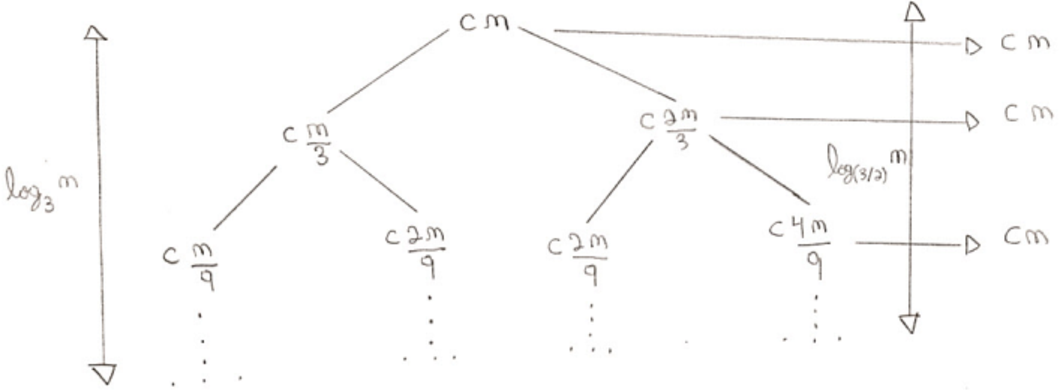
\includegraphics[width=0.7\textwidth]{images/4_4_6_1.pdf}
\end{center}

The tree is complete until level $\log_3 n$. The cost of the tree from the root
to level $\log_3 n$ is
\[
  \sum_{i = 0}^{\log_3 n} cn = cn \log_3 n,
\]
which is $\Omega(n \lg n)$.
\end{framed}

\newpage

\item[4.4{-}7]{Draw the recursion tree for $T(n) = 4T(\floor{n/2}) + cn$, where
$c$ is a constant, and provide a tight asymptotic bound on its solution. Verify
your bound by the substitution method.}

\begin{framed}
Since floors/ceiling usually do not matter, we will draw a recursion tree for
the recurrence $T(n) = 4T(n/2) + cn$.

\begin{center}
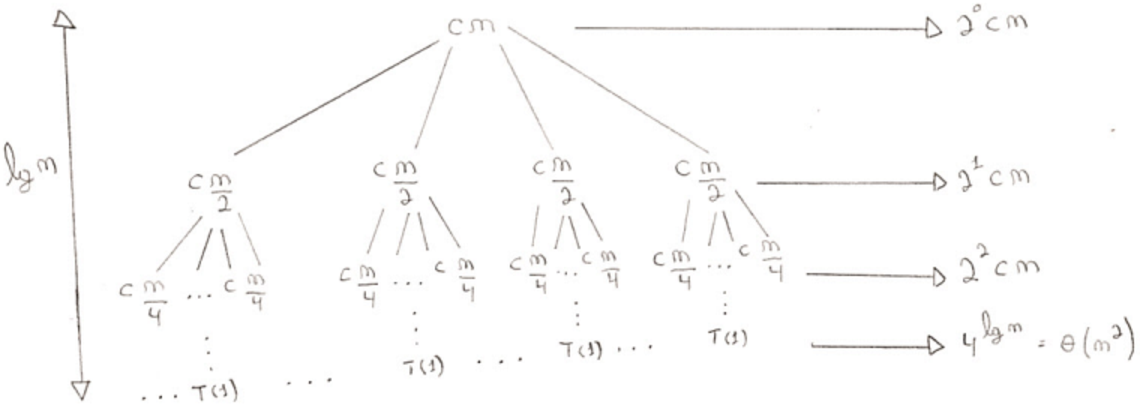
\includegraphics[width=0.9\textwidth]{images/4_4_7_1.pdf}
\end{center}

The number of nodes at depth $i$ is $4^i$. Since subproblem size reduce by
a factor of 2, each node at depth $i$, for $i = 0, 1, 2, \dots, \lg n - 1$,
has a cost of $c (n/2^i)$. Thus, the total cost over all nodes at depth
$i$, for $i = 0, 1, 2, \dots, \lg n - 1$, is $(4/2)^i cn = 2^i cn$. The bottom
level has $4^{\lg n} = n^2$ nodes, each contributing cost $T(1)$, for a total
cost of $n^2 T(1) = \Theta(n^2)$.

The cost of the entire tree is
\[
\sum_{i = 0}^{\lg n - 1} (2^i cn) + \Theta(n^2)
= cn \frac{2^{\lg n} - 1}{2 - 1} + \Theta(n^2)
= cn (n - 1) + \Theta(n^2)
= cn^2 - cn + \Theta(n^2)
= \Theta(n^2).
\]

Lets verify with the substitution method. Our guess for an upper bound is
\[
T(n) \le dn^2 - en \; \Forall n \ge n_0,
\]
where $d$, $e$, and $n_0$ are positive constants. Substituting into the
recurrence yields
\begin{equation*}
\begin{aligned}
  T(n) &\le 4\left(d \Bigl\lfloor\frac{n}{2}\Bigl\rfloor^2 -e \frac{n}{2}\right) + cn\\
       &\le 4\left(d \left(\frac{n}{2}\right)^2 -e \frac{n}{2}\right) + cn\\
       &=   4\left(d \frac{n^2}{4} -e \frac{n}{2}\right) + cn\\
       &=   d n^2 -2en + cn\\
       &=   d n^2 - en - en + cn\\
       &\le   d n^2 - en,
\end{aligned}
\end{equation*}
where the last step holds as long as $e \ge c$.

Our guess for a lower bound is
\[
T(n) \ge dn^2 \; \Forall n \ge n_0,
\]
where $d$, and $n_0$ are positive constants. Substituting into the
recurrence yields
\begin{equation*}
\begin{aligned}
  T(n) &\ge 4d \Bigl\lfloor\frac{n}{2}\Bigl\rfloor^2 + cn\\
       &\ge 4d \left(\frac{n}{2} - 1\right)^2 + cn\\
       &=   4d \left( \frac{n^2}{4} - n + 1 \right) + cn\\
       &=   d n^2 - 4dn + 4d + cn\\
       &=   d n^2 - (4d - c)n + 4d
\end{aligned}
\end{equation*}
where the last step holds as long as $4d - c \ge 4$ and $n_0 \ge d$.
\end{framed}

\newpage

\item[4.4{-}8]{Use a recursion tree to give an asymptotically tight solution to
the recurrence $T(n) = T(n - a) + T(a) + cn$, where $a \ge 1$ and $c > 0$ are
constants.}

\begin{framed}
Figure below ilustrates the recursion tree $T(n) = T(n - a) + T(a) + cn$.

\begin{center}
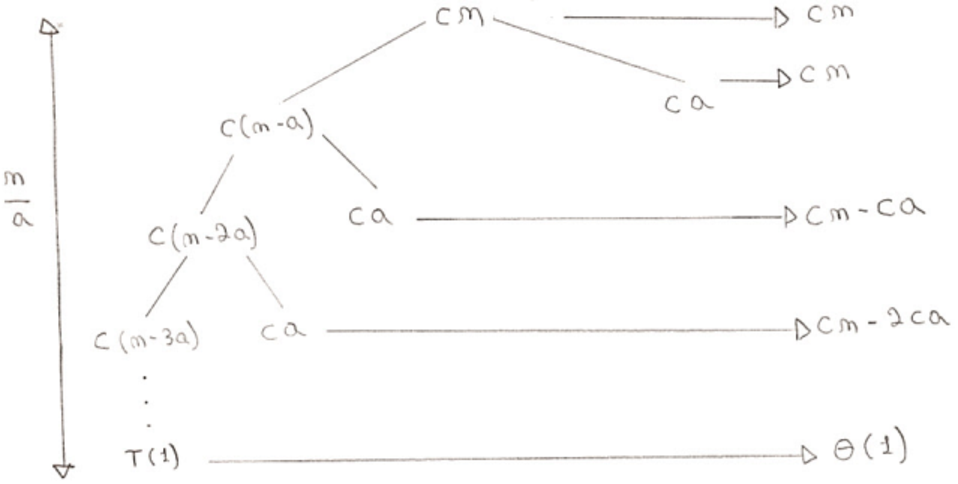
\includegraphics[width=0.7\textwidth]{images/4_4_8_1.pdf}
\end{center}

The height of the tree is $n/a$. Each level $i$, for $i = 1, 2, \dots, (n/a)$,
has two nodes, one that costs $c(n - ia)$ and another that costs $T(a) = ca$.
Thus, the cost over the nodes at depth $i$, for $i = 1, 2, \dots, (n/a)$, is
$c(n - a) + ca$. The root level, at deph 0, has a single node that costs $cn$.

The cost of the entire tree is
\begin{equation*}
\begin{aligned}
  T(n) &= cn + \sum_{i = 1}^{n/a} (c (n - ia) + ca)\\
       &= cn + \sum_{i = 1}^{n/a} cn - \sum_{i = 1}^{n/a} cia + \sum_{i = 1}^{n/a} ca\\
       &= cn + c\frac{n^2}{a} - \frac{cn (a + n)}{2a} + cn\\
       &= c \frac{n^2}{a} - c\frac{n^2}{2a} - c \frac{n}{2} + 2cn\\
       &= c \frac{n^2}{2a} + \frac{3}{2} cn\\
       &= \Theta(n^2).
\end{aligned}
\end{equation*}

Lets verify with the substitution method. Our guess for an upper bound is
\[
T(n) \le cn^2 \; \Forall n \ge n_0,
\]
where $c$ and $n_0$ are positive constants. Substituting into the
recurrence yields
\begin{equation*}
\begin{aligned}
  T(n) &\le c (n^2 - 2an + a^2) + ca + cn\\
       &=   cn^2 - c (2an - a - n - a^2)\\
       &\le cn^2,
\end{aligned}
\end{equation*}
where the last step holds as long as $n_0 \ge a$.

Our guess for a lower bound is
\[
  T(n) \ge \frac{c}{2a} n^2 \; \Forall n \ge n_0,
\]
where $c$, and $n_0$ are positive constants. Substituting into the
recurrence yields
\begin{equation*}
\begin{aligned}
  T(n) &\ge \frac{c}{2a} (n - a)^2 + ca + cn\\
       &=   \frac{c}{2a} (n^2 - 2an + a^2) + ca + cn\\
       &=   \frac{c}{2a} n^2 - cn + \frac{1}{2} ca + ca + cn\\
       &=   \frac{c}{2a} n^2 + \frac{3}{2} ca\\
       &\ge \frac{c}{2a} n^2.
\end{aligned}
\end{equation*}
\end{framed}

\newpage

\item[4.4{-}9]{Use a recursion tree to give an asymptotically tight solution to
the recurrence $T(n) = T(\alpha n) + T((1 - \alpha) n) + cn$, where $\alpha$ is
a constant in the range $0 < \alpha < 1$ and $c > 0$ is also a constant.}

\begin{framed}
Let $\alpha \ge 1 - \alpha$. Figure below ilustrates the recursion tree
$T(n) = T(\alpha n) + T((1 - \alpha n) n) + cn$.

\begin{center}
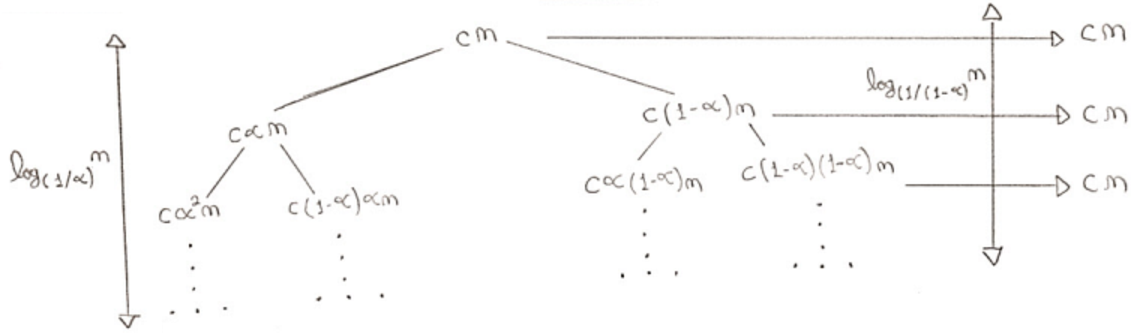
\includegraphics[width=0.8\textwidth]{images/4_4_9_1.pdf}
\end{center}

If it were a complete tree, all the $\log_{1 - \alpha} n$ levels would cost $cn$
and the entire tree $cn \log_{1 - \alpha} n$. Thus,
$T(n) = O(n \log_{1 - \alpha} n) = O(n \lg n)$. The tree is complete until level
$\log_{1/(1 - \alpha)} n$. The cost of the tree from the root to level
$\log_{1/(1 - \alpha)} n$ is
\[
  \sum_{i = 0}^{\log_{1/(1 - \alpha)} n} cn
  = \left(\sum_{i = 1}^{\log_{1/(1 - \alpha)} n} cn\right) + cn
  = cn (\log_{1/(1 - \alpha)} n) + cn,
\]
which is $\Omega(n \log_{1/(1 - \alpha)} n)$ = $\Omega(n \lg n)$.

Lets verify with the substitution method. Our guess for an upper bound is
\[
T(n) \le d n \lg n \; \Forall n \ge n_0,
\]
where $d$ and $n_0$ are positive constants. Substituting into the
recurrence yields
\begin{equation*}
\begin{aligned}
  T(n) &\le d \alpha n \lg (\alpha n) + d (1 - \alpha) n \lg ((1 - \alpha) n) + dn\\
       &=   d \alpha n \lg \alpha + d \alpha n \lg n + d (1 - \alpha) n \lg (1 - \alpha) + d (1 - \alpha) n \lg n + cn\\
       &=   d \alpha n \lg \alpha + d \alpha n \lg n + d (1 - \alpha) n \lg (1 - \alpha) + d n \lg n - d \alpha n \lg n + cn\\
       &=   d n \lg n + dn (\alpha \lg \alpha + (1 - \alpha) \lg (1 - \alpha)) + cn\\
       &\le d n \lg n,
\end{aligned}
\end{equation*}
where the last step holds as long as $d(\alpha \lg \alpha + (1 - \alpha) \lg (1 - \alpha)) + c \le 0$.

Our guess for a lower bound is
\[
  T(n) \ge d n \lg n \; \Forall n \ge n_0,
\]
where $d$, and $n_0$ are positive constants. Substituting into the
recurrence yields
\begin{equation*}
\begin{aligned}
  T(n) &\ge d \alpha n \lg (\alpha n) + d (1 - \alpha) n \lg ((1 - \alpha) n) + dn\\
       &=   d \alpha n \lg \alpha + d \alpha n \lg n + d (1 - \alpha) n \lg (1 - \alpha) + d (1 - \alpha) n \lg n + cn\\
       &=   d \alpha n \lg \alpha + d \alpha n \lg n + d (1 - \alpha) n \lg (1 - \alpha) + d n \lg n - d \alpha n \lg n + cn\\
       &=   d n \lg n + dn (\alpha \lg \alpha + (1 - \alpha) \lg (1 - \alpha)) + cn\\
       &\ge d n \lg n,
\end{aligned}
\end{equation*}
where the last step holds as long as $d(\alpha \lg \alpha + (1 - \alpha) \lg (1 - \alpha)) + c \ge 0$.
\end{framed}

\end{enumerate}

\newpage

\section{The master method for solving recurrences}

\begin{enumerate}

\item[4.5{-}1]{Use the master method to give tight asymptotic bounds for the
following recurrences.

\begin{enumerate}
  \item[a.] $T(n) = 2T(n/4) + 1$.
  \item[b.] $T(n) = 2T(n/4) + \sqrt{n}$.
  \item[c.] $T(n) = 2T(n/4) + n$.
  \item[d.] $T(n) = 2T(n/4) + n^2$.
\end{enumerate}
}

\begin{framed}
\begin{enumerate}
  \item[(a)] Case 1 applies. $T(n) = \Theta(n^{\log_4{2}}) = \Theta(\sqrt{n})$.
  \item[(b)] Case 2 applies. $T(n) = \Theta(n^{\log_4{2}} \lg n) = \Theta(\sqrt{n} \lg n)$.
  \item[(c)] Case 3 applies. $T(n) = \Theta(n)$.
  \item[(d)] Case 3 applies. $T(n) = \Theta(n^2)$.
\end{enumerate}
\end{framed}

\item[4.5{-}2]{Professor Caesar wishes to develop a matrix-multiplication
algorithm that is asymptotically faster than Strassen's algorithm. His algorithm
will use the divide-and-conquer method, dividing each matrix into pieces of
size $n/4 \times n/4$, and the divide and combine steps together will take
$\Theta(n^2)$ time. He needs to determine how many subproblems his algorithm has
to create in order to beat Strassen's algorithm. If his algorithm creates $a$
subproblems, then the recurrence for the running time $T(n)$ becomes
$T(n) = a T(n/4) + \Theta(n^2)$. What is the largest integer value of $a$ for
which Professor Caesar's algorithm would be asymptotically faster than
Strassen's algorithm?}

\begin{framed}
Strassen's algorithm costs $\Theta(n^{\lg 7})$. The cost of $T(n)$ is stated
below.
\begin{itemize}
  \item If $a < 16$, Case 3 applies. $T(n) = \Theta(n^2) = o(n^{\lg 7})$.
  \item If $a = 16$, Case 2 applies. $T(n) = \Theta(n^2 \lg n) = o(n^{\lg 7})$.
  \item If $a > 16$, Case 1 applies. $T(n) = \Theta(n^{\log_4{a}}) = o(n^{\lg 7})$ when $a < 49$.
\end{itemize}
Thus, the largest integer value of $a$ is 48.
\end{framed}

\item[4.5{-}3]{Use the master method to show that the solution to the
binary-search recurrence $T(n) = T(n/2) + \Theta(1)$ is $T(n) = \Theta(\lg n)$.
(See Exercise 2.3-5 for a description of binary search.)}

\begin{framed}
We have
\[
n^{\log_b a} = n^{\lg 1} = \Theta(1) = f(n).
\]
Thus, Case 2 applies. $T(n) = \Theta(\lg n)$.
\end{framed}

\newpage

\item[4.5{-}4]{Can the master method be applied to the recurrence
$T(n) = 4 T(n/2) + n^2 \lg n$? Why or why not? Give an asymptotic upper bound
for this recurrence.}

\begin{framed}
We have
\[
  f(n) = n^2 \lg n,
\]
and
\[
n^{\log_b a} = n^{\log_2 4} = \Theta(n^2),
\]
which is larger than $f(n)$, but not polynomially larger. Thus, we cannot use the
master method to solve this recurrence.

We can use a recursion tree to guess the cost of $T(n)$ and verify with the
substitution method. Figure below ilustrates the recursion tree of
$T(n) = 4 T(n/2) + n^2 \lg n$.

\begin{center} Figure here. \end{center}

The tree has $\lg n$ levels and the number of nodes at depth $i$ is $4^i$. Each
node at depth $i$ has a cost $c((n/2^i)^2) \lg(n) = 1/4^i c n^2 \lg n$. Thus,
the total cost at depth $i$ is $4^i \times 1/4^i c n^2 \lg n = c n^2 \lg n$.

The cost of the entire tree is
\[
  \sum_{i = 0}^{\lg n} c n^2 \lg n = O(n^2 \lg^2 n).
\]

Lets verify with the substitution method. Our guess is
\[
T(n) \le cn^2\lg^2 n \; \Forall n \ge n_0,
\]
where $c$ and $n_0$ are positive constants. Substituting into the
recurrence yields
\begin{equation*}
\begin{aligned}
  T(n) &\le 4c \left(\left(\frac{n}{2}\right)^2 \lg^2{\left(\frac{n}{2}\right)}\right) + n^2 \lg n\\
       &=   4c \left(\frac{n^2}{4} \lg{\left(\frac{n}{2}\right)}\lg{\left(\frac{n}{2}\right)}\right) + n^2 \lg n\\
       &=   c n^2 \lg{\left(\frac{n}{2}\right)}\lg{\left(\frac{n}{2}\right)} + n^2 \lg n\\
       &=   c n^2 \lg{\left(\frac{n}{2}\right)}\lg n - c n^2 \lg{\left(\frac{n}{2}\right)} + n^2 \lg n\\
       &=   c n^2 \lg^2 n - c n^2 \lg n - c n^2 \lg n + c n^2 + n^2 \lg n\\
       &\le c n^2 \lg^2 n,
\end{aligned}
\end{equation*}
where the last step holds as long as $c \ge 1$.

\end{framed}

\item[4.5{-}5]{Consider the regularity condition $a f(n/b) \ge c f(n)$ for some
constant $c < 1$, which is part of case 3 of the master theorem. Give an example
of constants $a \ge 1$ and $b > 1$ and a function $f(n)$ that satisfies all
the conditions in case 3 of the master theorem except the regularity
condition.}

\begin{framed}
Let $a = 1$, $b = 2$, and $f(n) = n \cos n$. We have
\[
  n^{\log_b a} = n^{\log_2 1} = \Theta(1),
\]
which is polynomially smaller than $f(n)$ and satisfies the primary condition of
Case 3. However, we have
\[
  a f\left(\frac{n}{b}\right) \le c f(n) \rightarrow \frac{n}{2} \cos\left(\frac{n}{2}\right) \le c ( n \cos n ),
\]
which is not valid for some constant $c < 1$ and all sufficiently large $n$
since $\cos(\cdot)$ is not monotonic. Thus, it satisfies the primary condition
of Case 3, but not the regularity condition
\end{framed}

\end{enumerate}

\newpage

\section*{Problems}
\addcontentsline{toc}{section}{\protect\numberline{}Problems}%

\begin{enumerate}

\item[4{-}1]{\textbf{\emph{Recurrence examples}}\\
Give asymptotic upper and lower bounds for $T(n)$ in each of the following
recurrences. Assume that $T(n)$ is constant for $n \ge 2$. Make your bounds as
tight as possible, and justify your answers.

\begin{enumerate}
  \item [a.] $2T(n/2) + n^4$.
  \item [b.] $T(7n/10) + n$.
  \item [c.] $16T(n/4) + n^2$.
  \item [d.] $7T(n/3) + n^2$.
  \item [e.] $7T(n/2) + n^2$.
  \item [f.] $2T(n/4) + \sqrt{n}$.
  \item [g.] $T(n - 2) + n^2$.
\end{enumerate}
}

\begin{framed}
\begin{enumerate}
  \item[(a)] We use the master method. Case 3 applies, since $n^{\lg 2} = n$ is
    polynomially smaller than $f(n)$. Thus, $T(n) = \Theta(n^4)$.
  \item[(b)] We use the master method. Case 3 applies, since
    $n^{\log_{10/7} 1} = 1$ is polynomially smaller than $f(n)$. Thus,
    $T(n) = \Theta(n)$.
  \item[(c)] We use the master method. Case 2 applies, since
    $n^{\log_4 14} = n^2 = \Theta(f(n))$. Thus, $T(n) = \Theta(n^2 \lg n)$.
  \item[(d)] We use the master method. Case 3 applies, since $n^{\log_3 7}$ is
    polynomially smaller than $f(n)$. Thus, $T(n) = \Theta(n^2)$.
  \item[(e)] We use the master method. Case 1 applies, since $n^{\lg 7}$ is
    polynomially larger than $f(n)$. Thus, $T(n) = \Theta(n^{\lg 7})$.
  \item[(f)] We use the master method. Case 2 applies, since
    $n^{\log_4 2} = \sqrt n = \Theta(f(n))$. Thus, $T(n) = \Theta(\sqrt n \lg n)$.
  \item[(g)] The recurrence has $n/2$ levels and depth $i$ costs $c(n - 2i)^2$.
    Thus, we have
    \[
      T(n) = \sum_{i = 0}^{n/2} c(n - 2i)^2
           = \sum_{i = 0}^{n/2} c(n^2 - 4ni + 4i^2)
           = c \left(\sum_{i = 0}^{n/2} n^2 - \sum_{i = 0}^{n/2} 4ni + \sum_{i = 0}^{n/2} 4i^2\right)
           = \Theta(n^3) - \Theta(n^2) + \Theta(n^3)
           = \Theta(n^3).
    \]
\end{enumerate}
\end{framed}

\newpage

\item[4{-}2]{\textbf{\emph{Parameter-passing costs}}\\
Throughout this book, we assume that parameter passing during procedure calls
takes constant time, even if an $N$-element array is being passed. This
assumption is valid in most systems because a pointer to the array is passed,
not the array itself.  This problem examines the implications of three
parameter-passing strategies:

\begin{enumerate}
  \item[1.] An array is passed by pointer. Time = $\Theta(1)$.
  \item[2.] An array is passed by copying. Time = $\Theta(N)$, where $N$ is the size
    of the array.
  \item[3.] An array is passed by copying only the subrange that might be accessed
    by the called procedure. Time = $\Theta(q - p + 1)$ if the subarray $A[p
    \dots q]$ is passed.
\end{enumerate}

\begin{enumerate}
  \item[a.] Consider the recursive binary search algorithm for finding a number
    in a sorted array (see Exercise 2.3-5). Give recurrences for the worst-case
    running times of binary search when arrays are passed using each of the
    three methods above, and give good upper bounds on the solutions of the
    recurrences. Let $N$ be the size of the original problem and $n$ be the size
    of a subproblem.
  \item[b.] Redo part (a) for the \textsc{Merge-Sort} algorithm from Section
    2.3.1.
\end{enumerate}
}

\begin{framed}
  \begin{enumerate}
    \item[a.] Binary search.
      \begin{enumerate}
        \item[1.] \emph{Array passed by pointer.}\\
          $T(n) = T(n/2) + \Theta(1)$.
          Case 2 of master method applies, since
          $n^{\lg 1} = 1 = f(n)$. Thus, $T(n) = \Theta(\lg n)$.
        \item[2.] \emph{Array passed by copying.}\\
          $T(n) = T(n/2) + \Theta(N) = T(n/4) + \Theta(N) + \Theta(N)$
          $= T(n/8) + \Theta(N) + \Theta(N) + \Theta(N)$
          $= \dots = \sum_{i = 0}^{\lg n} \Theta(N) = \Theta(n \lg n)$.
        \item[3.] \emph{Subarray passed by copying.}\\
          $T(n) = T(n/2) + \Theta(n)$.
          Case 3 of master method applies, since $n^{\lg 1} = 1$ is
          polynomially smaller than $f(n)$.\\
          Thus, $T(n) = \Theta(n)$.
      \end{enumerate}
    \item[b.] Merge sort.
      \begin{enumerate}
        \item[1.] \emph{Array passed by pointer.}\\
          $T(n) = T(\floor{n/2}) + T(\ceil{n/2}) + \Theta(n) \approx 2T(n/2) + \Theta(n)$.
          Case 2 of master method applies, since
          $n^{\lg 2} = n = f(n)$. Thus, $T(n) = \Theta(n \lg n)$.
        \item[2.] \emph{Array passed by copying.}\\
          $T(n) = 2T(n/2) + \Theta(N) = 4T(n/4) + 2\Theta(N) + \Theta(N)$
          $= 16T(n/8) + 4\Theta(N) + 2\Theta(N) + \Theta(N)$
          $= \dots = \sum_{i = 0}^{\lg n} 2^i \Theta(N) = \Theta(n^2)$.
        \item[3.] \emph{Subarray passed by copying.}\\
          $T(n) = 2T(n/2) + \Theta(n)$.
          Case 2 of master method applies, since
          $n^{\lg 2} = n = f(n)$. Thus, $T(n) = \Theta(n \lg n)$.
      \end{enumerate}
  \end{enumerate}
\end{framed}

\newpage

\item[4{-}3]{\textbf{\emph{More recurrence examples}}\\
Give asymptotic upper and lower bounds for $T(n)$ in each of the following
recurrences. Assume that $T(n)$ is constant for sufficiently small $n$. Make
your bounds as tight as possible, and justify your answers.

\begin{enumerate}
  \item[a.] $T(n) = 4T(n/3) + n \lg n$.
  \item[b.] $T(n) = 3T(n/3) + n / \lg n$.
  \item[c.] $T(n) = 4T(n/2) + n^2 \sqrt n$.
  \item[d.] $T(n) = 3T(n/3 - 2) + n/2$.
  \item[e.] $T(n) = 2T(n/2) + n / \lg n$.
  \item[f.] $T(n) = T(n/2) + T(n/4) + T(n/8) + n$.
  \item[g.] $T(n) = T(n - 1) + 1/n$.
  \item[h.] $T(n) = T(n - 1) + \lg n$.
  \item[i.] $T(n) = T(n - 2) + 1 / \lg n$.
  \item[j.] $T(n) = \sqrt n T(\sqrt n) + n$.
\end{enumerate}
}

\begin{framed}
  \begin{enumerate}
    \item[a.] We have $f(n) = n \lg n$ and $n^{\lg_b a} = n^{\log_3 4}$.
      Since $n \lg n = O(n^{\log_3(4) - 0.2})$, case 1 applies and we have
      $T(n) = \Theta(n^{\log_3 4})$.
    \item[b.] The tree has $\log_3 n$ levels and depth $i$, for $i = 0, 1,
      \dots, \log_3 n - 1$, costs $n/(\log_3 n - i)$. The cost of the entire
      tree is
      \[
        T(n) = \sum_{i = 0}^{\log_3 n - 1} \frac{n}{\log_3 n - i}
             = \sum_{i = 1}^{\log_3 n} \frac{n}{i}
             = n \sum_{i = 1}^{\log_3 n} \frac{1}{i}
             = n \cdot H_{\log_3 n}
             = n \cdot \Theta(\lg \log_3 n)
             = \Theta(n \lg \lg n).
      \]
      Skipped the proof.
    \item[c.] We have $f(n) = n^2 \sqrt n = n^{5/2}$ and
      $n^{\log_b a} = n^{\log_2 4} = n^2$. Since
      $n^{5/2} = \Omega(n^{2 + 1/2})$, we look at the regularity condition in
      case 3 of the master method. We have
      $af(n/b) = 4(n/2)^2 \sqrt{n/2} = (n^{5/2})/\sqrt 2 \le c n^{5/2}$ for
      $1/\sqrt 2 \le c < 1$. Case 3 applies and we have
      $T(n) = \Theta(n^2 \sqrt n)$.
    \item[d.]
      The tree has $\log_3 n$ levels and depth $i$, for
      $i = 0, 1, \dots, \log_3 n - 1$ costs $c (n/2) - 2 \cdot 3^i$. The cost of
      the entire tree is
      \[
        T(n) = \sum_{i = 0}^{\log_3 n - 1} \left(c \frac{n}{2} - 2 \cdot 3^i\right)
             = c \sum_{i = 0}^{\log_3 n - 1} \frac{n}{2} - 2 \sum_{i = 0}^{\log_3 n - 1} 3^i
             = \Theta(n \lg n).
      \]
      Our guess for the upper bound is
      \[
      T(n) \le c n \lg n \; \Forall n \ge n_0,
      \]
      where $c$ and $n_0$ are positive constants. Substituting into the recurrence
      yields
      \begin{equation*}
      \begin{aligned}
        T(n) &\le 3c \left(\frac{n}{3} - 2\right) \lg \left(\frac{n}{3} - 2\right) + \frac{n}{2}\\
             &=   c n \lg \left(\frac{n}{3} - 2\right) - 6c \lg \left(\frac{n}{3} - 2\right) + \frac{n}{2}\\
             &\le cn \lg \left(\frac{n}{3} - 2\right) - 6c \lg \left(\frac{n}{4}\right) + \frac{n}{2} & \text{($n \ge 24$)}\\
             &=   cn \lg \left(\frac{n}{3} - 2\right) - 6c \lg n - 12 c + \frac{n}{2}\\
             &<   cn \lg n - 6c \lg n - 12c + \frac{n}{2}\\
             &\le cn \lg n,
      \end{aligned}
      \end{equation*}
      where the last step holds as long as $-6c \lg n - 12c + n/2 \le 0$
      (skipped simplification).

      Our guess for the lower bound is
      \[
      T(n) \ge c n \lg n \; \Forall n \ge n_0,
      \]
      where $c$, and $n_0$ are positive constants. Substituting into the recurrence
      yields
      \begin{equation*}
      \begin{aligned}
        T(n) &\ge 3c \left(\frac{n}{3} - 2\right) \lg \left(\frac{n}{3} - 2\right) + \frac{n}{2}\\
             &=   c n \lg \left(\frac{n}{3} - 2\right) - 6c \lg \left(\frac{n}{3} - 2\right) + \frac{n}{2}\\
             &\ge cn \lg \left(\frac{n}{4}\right) - 6c \lg \left(\frac{n}{3} - 2\right) + \frac{n}{2} & \text{($n \ge 24$)}\\
             &=   cn \lg n - 2cn - 6c \lg \left(\frac{n}{3} - 2\right) + \frac{n}{2}\\
             &\ge cn \lg n,
      \end{aligned}
      \end{equation*}
      where the last step holds as long as $-2cn - 6c \lg (n/3 - 2) + n/2 \ge 0$
      (skipped simplification).
    \item[e.] The tree has $\lg n$ levels and depth $i$, for $i = 0, 1,
      \dots, \lg n - 1$, costs $n/(\lg n - i)$. The cost of the entire
      tree is
      \[
        T(n) = \sum_{i = 0}^{\lg n - 1} \frac{n}{\lg n - i}
             = \sum_{i = 1}^{\lg n} \frac{n}{i}
             = n \sum_{i = 1}^{\lg n} \frac{1}{i}
             = n \cdot H_{\lg n}
             = n \cdot \Theta(\lg \lg n)
             = \Theta(n \lg \lg n).
      \]
      Skipped the proof.
    \item[f.] The tree has $\lg n$ levels, but is not complete. Considering
      only the levels in which the tree is complete, depth $i$, for
      $i = 1, 2, \dots, \log_8 n$, costs $(7/8)^i cn$. Thus, the cost of the
      entire tree is at most
      \[
        T(n) \le \sum_{i=0}^{\lg n - 1} \left( \left(\frac{7}{8}\right)^i cn \right)
             = cn \sum_{i=0}^{\lg n - 1} \left( \left(\frac{7}{8}\right)^i \right)
             = cn \frac{1 - \left(\frac{7}{8}\right)^{\lg n}}{1 - \frac{7}{8}}
             = cn \frac{1 - n^{\lg 7 - 3}}{\frac{1}{8}}
             = 8cn - 8cn^{\lg 7 - 2}
             = O(n).
      \]
      Our guess for the upper bound is
      \[
      T(n) \le c n \; \Forall n \ge n_0,
      \]
      where $c$ and $n_0$ are positive constants. Substituting into the recurrence
      yields
      \begin{equation*}
      \begin{aligned}
        T(n) &\le c \frac{n}{2} + c \frac{n}{4} + c \frac{n}{8}\\
             &= \frac{7}{8} cn + n\\
             &\le cn,
      \end{aligned}
      \end{equation*}
      where the last step holds as long as $c \ge 8$.

      Our guess for the lower bound is
      \[
      T(n) \ge c n \; \Forall n \ge n_0,
      \]
      where $c$ and $n_0$ are positive constants. Substituting into the recurrence
      yields
      \begin{equation*}
      \begin{aligned}
        T(n) &\ge c \frac{n}{2} + c \frac{n}{4} + c \frac{n}{8}\\
             &= \frac{7}{8} cn + n\\
             &\ge cn,
      \end{aligned}
      \end{equation*}
      where the last step holds as long as $c \le 8$.
    \item[g.] The tree has $n$ levels and depth $i$, for
      $i = 1, 2, \dots, n - 1$, costs $1/(n - i)$. The cost of the entire tree
      is
      \[
        \sum_{i = 0}^{n - 1} \frac{1}{n - i} = \sum_{i = 1}^{n} \frac{1}{i} = H_n = \Theta(\lg n).
      \]
      Skipped the proof.
    \item[h.] The tree has $n$ levels and depth $i$, for
      $i = 1, 2, \dots, n - 1$, costs $\lg(n - i)$. The cost of the entire tree
      is
      \[
        \sum_{i = 0}^{n - 1} \lg(n - i) = \sum_{i = 1}^{n} \lg i = \lg(n!) = \Theta(n \lg n).
      \]
      Skipped the proof.
    \item[i.] Skipped.
    \item[j.] Skipped.
  \end{enumerate}
\end{framed}

\newpage

\item[4{-}4]{\textbf{\emph{Fibonacci numbers}}\\
This problem develops properties of the Fibonacci numbers, which are defined by
recurrence (3.22). We shall use the technique of generating functions to solve
the Fibonacci recurrence. Define the generating function (or formal power
series) $\mathcal{F}$ as

\begin{equation*}
\begin{aligned}
  \mathcal{F}(z) &= \sum_{i = 0}^\infty F_i z^i
                 &= 0 + z + z^2 + 2z^3 + 3z^4 + 5z^5 + 8z^6 + 13z^7 + 21z^8 + \dots,
\end{aligned}
\end{equation*}
where $F_i$ is the $i$th Fibonacci number.

\begin{enumerate}
  \item[a.] Show that $\mathcal{F}(z) = z + z \mathcal{F}(z) + z^2 \mathcal{F}(z)$.
  \item[b.] Show that
    \begin{equation*}
    \begin{aligned}
      \mathcal{F}(z) &= \frac{z}{1 - z - z^2}\\
                     &= \frac{z}{(1 - \phi z)(1 - \hat\phi z)}\\
                     &= \frac{1}{\sqrt 5} \left( \frac{1}{1 - \phi z} - \frac{1}{1 - \hat\phi z} \right),
    \end{aligned}
    \end{equation*}
    where
    \[
      \phi = \frac{1 + \sqrt 5}{2} = 1.61803 \dots
    \]
    and
    \[
      \hat\phi = \frac{1 - \sqrt 5}{2} = 0.61803 \dots .
    \]
  \item[c.] Show that
    \begin{equation*}
    \begin{aligned}
      \mathcal{F}(z) &= \sum_{i = 0}^\infty \frac{1}{\sqrt 5} (\phi^i - \hat\phi^i) z^i.
    \end{aligned}
    \end{equation*}
  \item[d.] Use part (c) to prove that $F_i = \phi^i/\sqrt{5}$ for $i > 0$,
    rounded to the nearest integer.\\(Hint: Observe that $|\hat\phi| < 1$.)
\end{enumerate}
}

\begin{framed}
  \begin{enumerate}
    \item[a.]
      \begin{equation*}
      \begin{aligned}
        \mathcal{F}(z) &= \sum_{i = 0}^{\infty} F_i z^i\\
                       &= 0 + z + \sum_{i = 2}^{\infty} (F_{(i - 1)} + F_{(i - 2)}) z^i\\
                       &= z + \sum_{i = 2}^{\infty} F_{(i - 1)} z^i + \sum_{i = 2}^{\infty} F_{(i - 2)} z^i\\
                       &= z + \sum_{i = 1}^{\infty} F_i z^{i + 1} + \sum_{i = 0}^{\infty} F_i z^{i + 2}\\
                       &= z + \sum_{i = 0}^{\infty} F_i z^{i + 1} + \sum_{i = 0}^{\infty} F_i z^{i + 2} & \text{(since $F_0 = 0$)}\\
                       &= z + z \sum_{i = 0}^{\infty} F_i z^{i} + z^2 \sum_{i = 0}^{\infty} F_i z^{i}\\
                       &= z + z \mathcal{F}(z) + z^2 \mathcal{F}(z).
      \end{aligned}
      \end{equation*}
    \newpage
    \item[b.]
      \begin{equation*}
        \begin{aligned}
          \mathcal{F}(z) &= \mathcal{F}(z) \cdot \frac{1 - z - z^2}{1 - z - z^2}\\
                         &= \frac{\mathcal{F}(z) - z\mathcal{F}(z) - z^2 \mathcal{F}(z)}{1 - z - z^2}\\
                         &= \frac{\mathcal{F}(z) - (z + z \mathcal{F}(z) + z^2 \mathcal{F}(z)) + z}{1 - z - z^2}\\
                         &= \frac{\mathcal{F}(z) - \mathcal{F}(z) + z}{1 - z - z^2} & \text{(from previous proof)}\\
                         &= \frac{z}{1 - z - z^2}\\
                         &= \frac{z}{1 - (\phi + \hat\phi)z + \phi \hat\phi z^2}
                         & \text{(since $\phi + \hat\phi = 1$ and $\phi \hat\phi = -1$)}\\
                         &= \frac{z}{(1 - \phi z)(1 - \hat\phi z)}\\
                         &= \frac{1}{\sqrt 5} \left(\frac{1}{1 - \phi z} - \frac{1}{1 - \hat\phi z}\right).
                         & \text{(skipped this proof)}
        \end{aligned}
      \end{equation*}
    \item[c.]
      \begin{equation*}
        \begin{aligned}
          \mathcal{F}(n) &= \frac{1}{\sqrt 5} \left(\frac{1}{1 - \phi z} - \frac{1}{1 - \hat\phi z}\right)\\
                         &= \frac{1}{\sqrt 5} \left(\sum_{i = 0}^{\infty} (\phi z)^i - \sum_{i = 0}^{\infty} (\hat\phi z)^i\right)
                         & \text{(by equation A.6, geometric series)}\\
                         &= \frac{1}{\sqrt 5} \sum_{i = 0}^{\infty} \left( (\phi z)^i - (\hat\phi z)^i \right)\\
                         &= \sum_{i = 0}^{\infty} \frac{1}{\sqrt 5} (\phi^i - \hat\phi^i) z^i.
        \end{aligned}
      \end{equation*}
    \item[d.] Skipped.
  \end{enumerate}
\end{framed}

\newpage

\item[4{-}5]{\textbf{\emph{Chip testing}}\\
Professor Diogenes has $n$ supposedly identical integrated-circuit chips that in
principle are capable of testing each other. The professor's test jig
accommodates two chips at a time. When the jig is loaded, each chip tests the
other and reports whether it is good or bad. A good chip always reports
accurately whether the other chip is good or bad, but the professor cannot trust
the answer of a bad chip. Thus, the four possible outcomes of a test are as
follows:

\begin{tabular}{lll}
  Chip $A$ says & Chip $B$ says & Conclusion\\
  \toprule
  $B$ is good & $A$ is good & both are good, or both are bad\\
  $B$ is good & $A$ is bad  & at least one is bad\\
  $B$ is bad  & $A$ is good & at least one is bad\\
  $B$ is bad  & $A$ is bad  & at least one is bad
\end{tabular}

\begin{enumerate}
  \item[a.] Show that if at least $n/2$ chips are bad, the professor cannot
    necessarily determine which chips are good using any strategy based on this
    kind of pairwise test. Assume that the bad chips can conspire to fool the
    professor.
  \item[b.] Consider the problem of finding a single good chip from among
    $n$ chips, assuming that more than $n/2$ of the chips are good. Show that
    $\floor{n/2}$ pairwise tests are sufficient to reduce the problem to one of
    nearly half the size.
  \item[c.] Show that the good chips can be identified with $\Theta(n)$ pairwise
    tests, assuming that more than $n/2$ of the chips are good. Give and solve
    the recurrence that describes the number of tests.
\end{enumerate}
}

\begin{framed}
  \begin{enumerate}
    \item[a.] Let $n_g$ be the number of good chips and $n_b$ the
      number of bad chips, such that $n_b \ge n_g$ and $n_g
      + n_b = n$. If the bad chips decide evaluate the others incorrectly
      (good as bad and bad as good), the professor will have the following
      result:

      \begin{tabular}{lll}
        Chip state & Tested as good & Tested as bad\\
        \toprule
        Good       & $n_g - 1$ times & $n_b$ times\\
        Bad        & $n_b - 1$ times & $n_g$ times\\
      \end{tabular}

      In this jig test, the number of good tests of the bad chips will be equal
      or greater the number of good tests of the good chips, which will confuse
      the professor.
    \item[b.] Group the chips in groups of two (if $n$ is odd, put the remaining
      chip in the next subproblem), making a total of $\floor{n/2}$ groups, and
      evaluate each group in the test jig. For each test, do the following:

      \begin{tabular}{llll}
        Group type & Chip $A$ says & Chip $B$ says & Conclusion\\
        \toprule
        1 & $B$ is good & $A$ is good & keep one of them\\
        2 & $B$ is good & $A$ is bad  & discard both\\
        3 & $B$ is bad  & $A$ is good & discard both\\
        4 & $B$ is bad  & $A$ is bad  & discard both
      \end{tabular}

      For each test where at least one of the chips is evaluated as bad (group
      types 2, 3, and 4), we known that at least one of them is truly bad. Thus,
      we can safely discard both and assure that the majority of the remaining
      chips are good. As for the groups where both of the chips are evaluated as
      good (group type 1), we can assure that at least half of these groups are
      composed by truly good chips, thus keeping one of them is enough to assure
      that the subproblem will have at least half of good chips. The case where
      exactly half of the groups of type 1 is composed by good chips only can
      happen when $n$ is odd and the remaining chip that we previously added to
      the subproblem must be good, thus assuring that the majority of the chips
      from the subproblem is good. Also, since the number of groups is
      $\floor{n/2}$, the algorithm will perform $\floor{n/2}$ tests and the
      subproblem will have at most $\ceil{n/2}$ chips.
    \item[c.] The recurrence of the above algorithm is
      \[
        T(n) = T\left(\Bigl\lceil\frac{n}{2}\Bigl\rceil\right) + \frac{n}{2}.
      \]
      We have that $f(n) = n/2$ and $n^{\log_b a} = n^{\log_2 1} = n^0 = 1$.
      Since $n/2 = \Omega(n^{0 + 0.5})$, we look at the regularity condition in
      case 3 of masther method. We have $a f(n/b) = n/4 \le c n/2$ for $1/2 \le
      c < 1$. Case 3 applies and we have $T(n) = \Theta(n/2) = \Theta(n)$.
  \end{enumerate}
\end{framed}

\newpage

\item[4{-}6]{\textbf{\emph{Monge arrays}}\\
An $m \times n$ array $A$ of real numbers is a \textbf{\emph{Monge array}} if
for all $i, j, k$, and $l$ such that $1 \le i < k \le m$ and
$1 \le j < l \le n$, we have
\[
  A[i, j] + A[k, l] \le A[i, l] + A[k, j].
\]
In other words, whenever we pick two rows and two columns of a Monge array and
consider the four elements at the intersections of the rows and the columns, the
sum of the upper-left and lower-right elements is less than or equal to the sum
of the lower-left and upper-right elements. For example, the following array is
Monge:

\begin{tabular}{ccccc}
10 & 17 & 13 & 28 & 23\\
17 & 22 & 16 & 29 & 23\\
24 & 28 & 22 & 34 & 24\\
11 & 13 & 6  & 17 & 7\\
45 & 44 & 32 & 37 & 23\\
36 & 33 & 19 & 21 & 6\\
75 & 66 & 51 & 53 & 34
\end{tabular}

\begin{enumerate}
  \item[a.] Prove that an array is Monge if and only if for all $i = 1, 2,
    \dots, m - 1$ and $j = 1, 2, \dots, n - 1$, we have:
    \[
      A[i, j] + A[i + 1, j + 1] \le A[i, j + 1] + A[i + 1, j].
    \]
    (Hint: For the ``if'' part, use induction separately on rows and columns.)
  \item[b.] The following array is not Monge. Change one element in order to
    make it Monge. (Hint: Use part(a).)

    \begin{tabular}{cccc}
      37 & 23 & 22 & 32\\
      21 & 6  & 7  & 10\\
      53 & 34 & 30 & 31\\
      32 & 13 & 9  & 6\\
      43 & 21 & 15 & 8
    \end{tabular}
  \item[c.] Let $f(i)$ be the index of the column containing the leftmost
    minimum element of row $i$. Prove that $f(1) \le f(2) \le \cdots \le f(m)$
    for any $m \times n$ Monge array.
  \item[d.] Here is a description of a divide-and-conquer algorithm that
    computes the leftmost minimum element in each row of an $m \times n$ Monge array $A$:

    \begin{quote}
      Construct a submatrix $A'$ of $A$ consisting of the even-numbered rows of
      $A$.  Recursively determine the leftmost minimum for each row of $A'$.
      Then compute the leftmost minimum in the odd-numbered rows of $A$.
    \end{quote}

    Explain how to compute the leftmost minimum in the odd-numbered rows of $A$
    (given that the leftmost minimum of the even-numbered rows is known) in
    $O(m + n)$ time.

  \item[e.] Write the recurrence describing the running time of the algorithm
    described in part (d). Show that it is $O(m + n \log m)$.
\end{enumerate}
}

\begin{framed}
  \begin{enumerate}
    \item[a.] The ``only if'' part is trivial. Since $k = i + 1, \dots, m$ and $l = j + 1, \dots, n$, we have
      \[
        A[i, j] + A[k, l] \le A[i, l] + A[k, j] \rightarrow A[i, j] + A[i + 1, j + 1] \le A[i, j + 1] + A[i + 1, j],
      \]

      For the ``if'' part, we first need to show
      \begin{equation}
        A[i, j] + A[i + 1, j + 1] \le A[i, j + 1] + A[i + 1, j] \rightarrow A[i, j] + A[k, j + 1] \le A[i, j + 1] + A[k, j]
        \label{eq:p_4_6}
      \end{equation}
      is valid for all $k > i$. The base case, which occurs when $k = i + 1$, is
      given. Thus, we have
      \[
        A[k, j] + A[k + 1, j + 1] \le A[k, j + 1] + A[k + 1, j].
      \]
      in which $k = i + 1, \dots, m - 1$. Now assume that the rhs of (1) holds for a given $k$
      \[
        A[i, j] + A[k, j + 1] \le A[i, j + 1] + A[k, j],
      \]
      then we have
      \[
        \underbrace{A[i, j] + A[k, j + 1]}_\text{assumption} +
        \underbrace{A[k, j] + A[k + 1, j + 1]}_\text{base case} \le
        \underbrace{A[i, j + 1] + A[k, j]}_\text{assumption} +
        \underbrace{A[k, j + 1] + A[k + 1, j]}_\text{base case},
      \]
      cancelling equal terms on both sides, we have
      \[
        A[i, j] + A[k + 1, j + 1] \le A[i, j + 1] + A[k + 1, j],
      \]
      which shows that it also holds for $k + 1$ and proves the inductive step.

      Then we need to show
      \begin{equation}
        A[i, j] + A[i + 1, j + 1] \le A[i, j + 1] + A[i + 1, j] \rightarrow A[i, j] + A[i + 1, l] \le A[i, l] + A[i + 1, j]
      \end{equation}
      is valid for all $l > j$. The base case, which occurs when $l = j + 1$, is
      given. Thus, we have
      \[
        A[i, l] + A[i + 1, l + 1] \le A[i, l + 1] + A[i + 1, l].
      \]
      in which $l = j + 1, \dots, n - 1$. Now assume that the rhs of (2) holds for a given $l$
      \[
        A[i, j] + A[i + 1, l] \le A[i, l] + A[i + 1, j],
      \]
      then we have
      \[
        \underbrace{A[i, j] + A[i + 1, l]}_\text{assumption} +
        \underbrace{A[i, l] + A[i + 1, l + 1]}_\text{base case} \le
        \underbrace{A[i, l] + A[i + 1, j]}_\text{assumption} +
        \underbrace{A[i, l + 1] + A[i + 1, l]}_\text{base case},
      \]
      cancelling equal terms on both sides, we have
      \[
        A[i, j] + A[i + 1, l + 1] \le  + A[i, l + 1] + A[i + 1, j],
      \]
      which shows that it also holds for $l + 1$ and proves the inductive step.

      From the ``if'' and ``only if'' proofs, we have
      \[
        A[i, j] + A[k, l] \le A[i, l] + A[k, j] \iff A[i, j] + A[i + 1, j + 1] \le A[i, j + 1] + A[i + 1, j].
      \]
      \item[b.] Let $M$ be the $m \times n$ matrix we want to make Monge. In
        this case, $m = 5$ and $n = 4$. From item (a), we know that, to be
        Monge, the following needs to hold:
        \begin{equation*}
        \begin{aligned}
        M[i, j] + M[i + 1, j + 1] \le M[i, j + 1] + M[i + 1, j] \; \Forall i = 1, 2, \dots, m - 1 \; \Forall j = 1, 2, \dots, n - 1,\\
        \end{aligned}
        \end{equation*}
      which implies
      \[
        M[i, j] + M[i + 1, j + 1] - M[i, j + 1] + M[i + 1, j] \le 0.
      \]
      Let $K$ be an $(m - 1) \times (n - 1)$ matrix where
      \[
        K[i, j] = M[i, j] + M[i + 1, j + 1] - M[i, j + 1] + M[i + 1, j].
      \]
      Thus, we have
      \[
      K =
      \begin{bmatrix}
      -1 &  2 & -7\\
      -4 & -5 & -2\\
       0 &  0 & -4\\
      -3 & -2 & -4
      \end{bmatrix}
      ,\]
    which shows that the problem is that
    $M[1, 2] + M[2, 3] - M[1, 3] + M[2, 2] = 2 > 0$.

    We can make $M$ monge by changing the element $M[1, 3]$ from $22$ to $24$,
    now becoming:
      \[
      M =
      \begin{bmatrix}
      37 & 23 & 24 & 32\\
      21 & 6  & 7  & 10\\
      53 & 34 & 30 & 31\\
      32 & 13 & 9  & 6\\
      43 & 21 & 15 & 8
      \end{bmatrix}
      .\]
    \item[c.] Lets assume that $f(i + 1) < f(i)$. From the definition of a Monge
      array, we have
      \[
        A[i, f(i + 1)] + A[i + 1, f(i)] \le A[i, f(i)] + A[i + 1, f(i + 1)],
      \]
      which is not possible since from the definition of $f(\cdot)$
      \[
        A[i, f(i + 1)] > A[i, f(i)],
      \]
      and
      \[
        A[i + 1, f(i)] \ge A[i + 1, f(i + 1)].
      \]
    \item[d.] We know from item (c) that $f(i - 1) \le f(i) \le f(i + 1)$. Thus,
      for each odd-numbered row $i$ of the matrix, we just need to find the
      leftmost minimum of row $i$ between the columns $f(i - 1)$ and $f(i + 1)$,
      which includes $f(i + 1) - f(i - 1) + 1$ elements. If $i$ corresponds to
      the first ($i = 1$) or the last ($i = m$) row of the matrix, consider
      $f(i - 1) = f(0) = 1$ or $f(i + 1) = f(m + 1) = m$. Since the matrix has
      $\ceil{m / 2}$ odd-numbered rows, finding the leftmost minimum of all of
      them takes
      \begin{equation*}
      \begin{aligned}
        \sum_{i = 1}^{\ceil{m/2}} (f(i + 1) - f(i - 1) + 1)
        &= \Bigl\lceil{\frac{m}{2}}\Bigl\rceil + \sum_{i = 1}^{\ceil{m/2}} (f(i + 1) - f(i - 1))\\
        &= O(m) + f(\ceil{m/2}) - f(1)\\
        &= O(m + n).
      \end{aligned}
      \end{equation*}
    \item[e.]
      Since we can partition the array in $O(1)$ (working with pointers), the
      recurrence can be written as
      \begin{equation*}
      \begin{aligned}
        T(m) &= T(m/2) + O(m + n)\\
             &= \sum_{i = 0}^{\lg m - 1} \left(cn + d \frac{m}{2^i}\right)\\
             &= cn \lg m + dm \sum_{i = 0}^{\lg m - 1} \frac{1}{2^i}\\
             &\le cn \lg m + dm \sum_{i = 0}^{\infty} (1/2)^i & \text{(infinity decreasing geometric series)}\\
             &= cn \lg m + dm \left(\frac{1}{1 - (1/2)}\right)\\
             &= cn \lg m + 2dm\\
             &= O(m + n \lg m).
      \end{aligned}
      \end{equation*}
  \end{enumerate}

\end{framed}

\end{enumerate}

\chapter{Probabilistic Analysis and Randomized Algorithms}

\section{The hiring problem}

\begin{enumerate}

\item[5.1{-}1]{Show that the assumption that we are always able to determine
which candidate is best, in line 4 of procedure \textsc{Hire-Assistant}, implies
that we know a total order on the ranks of the candidates.}

\begin{framed}
Let $A$ be the set of candidates in random order and $R$ the binary relation
``is better than or equal''. $R$ is a total order if
\begin{enumerate}
  \item $R$ is \textbf{reflexive}. That is, $a\;R\;a \; \Forall a \in A$;
  \item $R$ is \textbf{antisymmetric}. That is, $a\;R\;b$ and $b\;R\;a$ imply $a = b$;
  \item $R$ is \textbf{transitive}. That is, $a\;R\;b$ and $b\;R\;c$ imply $a\;R\;c$;
  \item $R$ is a \textbf{total relation}. That is, $a\;R\;b$ or $b\;R\;a \; \Forall a, b \in A$.
\end{enumerate}

The above properties are necessary because
  \begin{enumerate}
    \item if two different candidates have the same qualification, it is
      necessary so that they can be compared;
    \item if both $a$ is ``better than or equal'' than $b$ and $b$ is ``better
      than or equal'' than $a$ and they qualifications are not equal, we would
      not be able to choose one of them and still be hiring ``the best candidate
      we have seen so far'';
    \item if we hire $b$ because he is ``better than or equal'' than $a$ and
      then we hire $c$ because he is ``better than or equal'' than $b$ and $c$
      is not ``better than or equal'' than $a$, we are not hiring ``the best
      candidate we have seen so far'';
    \item if $R$ is not a total relation, we would not be able to compare any
      two candidates.
\end{enumerate}
\end{framed}

\item[5.1{-}2]{($\star$) Describe an implementation of the procedure \textsc{Random}(a, b)
that only makes calls to \textsc{Random}(0, 1). What is the expected running
time of your procedure, as a function of a and b?}

\begin{framed}
The pseudocode is stated below.\\
\begin{algorithm}[H]
\SetAlgoNoEnd\DontPrintSemicolon
\BlankLine
\SetKwFunction{algo}{RandomInterval}
\SetKwProg{myalg}{}{}{}
\myalg{\algo{a, b}}{%
\nl $flips = \ceil{\lg (b - a)}$\;
\nl $count = \infty$\;
\nl \While{$count > b$}{%
\nl   $count = 0$\;
\nl   \For{$i = 1$ \KwTo $flips$}{%
\nl     $count = count + (2^{i - 1} \cdot \texttt{Random}(0, 1))$\; } }
\nl \Return{$count + a$}\; }
\end{algorithm}

The expected running time is
\[
  \underbrace{2^{\ceil{\lg(b - a)}}/(b - a)}_\text{while loop} \cdot \underbrace{\ceil{\lg(b - a)}}_\text{for loop} < 2 \cdot \ceil{\lg(b - a)},
\]
where the last inequality is valid since $1 \le 2^{\ceil{\lg(b - a)}}/(b - a) < 2$.
\end{framed}

\item[5.1{-}3]{($\star$) Suppose that you want to output 0 with probability
$1/2$ and 1 with probability $1/2$.  At your disposal is a procedure
\textsc{Biased-Random}, that outputs either 0 or 1. It outputs 1 with some
probability $p$ and 0 with probability $1 - p$, where $0 < p < 1$, but you do
not know what $p$ is. Give an algorithm that uses \textsc{Biased-Random} as
a subroutine, and returns an unbiased answer, returning 0 with probability $1/2$
and 1 with probability $1/2$. What is the expected running time of your
algorithm as a function of $p$?}

\begin{framed}
The pseudocode is stated below.\\
\begin{algorithm}[H]
\SetAlgoNoEnd\DontPrintSemicolon
\BlankLine
\SetKwFunction{algo}{Random}
\SetKwProg{myalg}{}{}{}
\myalg{\algo{}}{%
\nl \While{$1$}{%
\nl   $r_1 = \texttt{Random}(0, 1)$\;
\nl   $r_2 = \texttt{Random}(0, 1)$\;
\nl   \If{$r_1 \neq r_2$}{%
\nl     \Return{$r_1$}\; } } }
\end{algorithm}

The expected running time is
\[
  \frac{1}{\underbrace{(1 - p) p}_\text{$(r_1, r_2) = (0, 1)$} + \underbrace{p (1 - p)}_\text{$(r_1, r_2) = (1, 0)$}} \cdot 1 = \frac{1}{2p (1- p)}.
\]
\end{framed}

\end{enumerate}

\newpage

\section{Indicator random variables}

\begin{enumerate}

\item[5.2{-}1]{In \textsc{Hire-Assistant}, assuming that the candidates are
presented in a random order, what is the probability that you hire exactly
one time? What is the probability that you hire exactly $n$ times?}

\begin{framed}
Since the initial dummy candidate is the least qualified,
\textsc{Hire-Assistant} will always hire the first candidate. It hires exacly
one time when the best candidate is the first to be interviewed. Thus, the
probability is $1/n$. To hire exactly $n$ times, the candidates has to be in
increasing order of quality. Since there are $n!$ possible orderings (each one
with equal probability of happening), the probability is $1/n!$.
\end{framed}

\item[5.2{-}2]{In \textsc{Hire-Assistant}, assuming that the candidates are
presented in a random order, what is the probability that you hire exactly
twice?}

\begin{framed}
The first candidate is always hired, thus the best qualified candidate cannot be
the first to be interviewed. Also, among all the candidates that are better
qualified than the first candidate, the best candidate must be interviewed first.
Otherwise, a third candidate will be hired between them. Now assume that the
first candidate to be interviewed is the $i$th best qualified, for $i = 2,
\dots, n$. This occurs with a probability of $1/n$. To hire exactly twice, the
best candidate must be the first to be interviewed among the $i - 1$ candidates
that are better qualified than candidate $i$. This occurs with a probability
of $1/(i - 1)$. Thus, the probability of hiring exactly twice is
\[
  \sum_{i = 2}^{n} \frac{1}{n} \frac{1}{i - 1} = \frac{1}{n} \sum_{i = 1}^{n - 1} \frac{1}{i} = \frac{1}{n} (\lg(n - 1) + O(1)).
\]
\end{framed}

\item[5.2{-}3]{Use indicator random variables to compute the expected value of
the sum of $n$ dice.}

\begin{framed}
Let $X_i$ be an indicator random variable of a dice coming up the number $i$. We
have $\text{Pr}\{X_i\} = 1/6$. Let $X$ be a random variable denoting the
result of throwing a dice. Then
\[
  \text{E}[X] = \sum_{i = 1}^{6} i \cdot \text{Pr}\{X_i\}
              = \sum_{i = 1}^{6} i \cdot \frac{1}{6}
              = \frac{1}{6} \sum_{i = 1}^{6} i
              = \frac{1}{6} \frac{6 \cdot 7}{2} = 3.5.
\]
By linearity of expectations, the expected value of the sum of $n$ dice is the
sum of the expected value of each dice. Thus,
\[
  \sum_{i = 1}^{n} \text{E}[X] = \sum_{i = 1}^{n} 3.5 = 3.5 \cdot n.
\]
\end{framed}

\item[5.2{-}4]{Use indicator random variables to solve the following problem,
which is known as the \textbf{\emph{hat-check problem}}. Each of $n$ customers
gives a hat to a hat-check person at a restaurant. The hat-check person
gives the hats back to the customers in a random order. What is the expected
number of customers who get back their own hat?}

\begin{framed}
Let $X_i$ be an indicator random variable of customer $i$ getting back his own
hat. We have
\[
\text{Pr}\{X_i\} = \text{E}[X_i] = 1/n.
\]
Let $X$ be a random variable denoting the number of customers who get back their
own hat. Then
\[
  X = X_1 + X_2 + \cdots + X_n,
\]
which implies
\begin{equation*}
\begin{aligned}
  \text{E}[X] &= \text{E}\left[\sum_{i = 1}^{n} X_i\right]\\
              &= \sum_{i = 1}^{n} \text{E}[X_i]\\
              &= \sum_{i = 1}^{n} \frac{1}{n}\\
              &= 1.
\end{aligned}
\end{equation*}
\end{framed}

\item[5.2{-}5]{Let $A[1, \dots, n]$ be an array of $n$ distinct numbers. If
$i < j$ and $A[i] > A[j]$, then the pair $(i, j)$ is called an
$\textbf{\emph{inversion}}$ of $A$. (See Problem 2-4 for more on inversions.)
Suppose that the elements of $A$ form a uniform random permutation of
$\langle 1, 2, \dots, n \rangle$. Use indicator random variables to compute
the expected number of inversions.}

\begin{framed}
Let $X_{ij}$ be an indicator random variable for the event that the pair
$(i, j)$ is inverted. Since $A$ forms a uniform random permutation, we have
\[
\text{Pr}\{X_{ij}\} = \text{Pr}\{\overline{X_{ij}}\} = 1/2,
\]
which implies
\[
  \text{E}[X_{ij}] = 1/2.
\]
Let $X$ be a random variable denoting the number of
inversions of $A$. Since there are $\binom{n}{2}$ possible pairs on $A$, each
with probability $1/2$ of being inverted, we have
\[
  \text{E}[X] = \binom{n}{2} \frac{1}{2} = \frac{n!}{2! \cdot (n - 2)!} \frac{1}{2} = \frac{n (n - 1)}{4}.
\]
\end{framed}

\end{enumerate}

\newpage

\section{Randomized algorithms}

\begin{enumerate}

\item[5.3{-}1]{Professor Marceau objects to the loop invariant used in the proof
of Lemma 5.5. He questions whether it is true prior to the first iteration. He
reasons that we could just as easily declare that an empty subarray contains
no 0-permutations. Therefore, the probability that an empty subarray
contains a 0-permutation should be 0, thus invalidating the loop invariant
prior to the first iteration. Rewrite the procedure \textsc{Randomize-In-Place}
so that its associated loop invariant applies to a nonempty subarray prior
to the first iteration, and modify the proof of Lemma 5.5 for your procedure.}

\begin{framed}
Just select a random element in the array and swap it with the first element.

\begin{algorithm}[H]
\SetAlgoNoEnd\DontPrintSemicolon
\BlankLine
  \SetKwFunction{algo}{Randomize-In-Place}
\SetKwProg{myalg}{}{}{}
\myalg{\algo{A}}{%
\nl $n = A.length$\;
\nl swap $A[1]$ with $A[\texttt{Random}(1, n)]$\;
\nl \For{$i = 2$ \KwTo $n - 1$}{%
\nl   swap $A[i]$ with $A[\texttt{Random}(i, n)]$\; } }
\end{algorithm}

The only difference in the proof of Lemma 5.5 is the initialization of the loop
invariant:
\begin{itemize}
  \item \textbf{Initialization.} Consider the situation just before the first
    loop iteration, so that $i = 2$. The loop invariant says that for each
    possible 1-permutation, the subarray $A[1, \dots, 1]$ contains this
    1-permutation with probability $(n - i + 1)/n! = (n - 1)!/n! = 1/n$. The
    subarray $A[1, \dots, 1]$ has a single element and this element was
    randomly choosed among the $n$ elements of the array. Thus, $A[1, \dots, 1]$
    contains this $1$-permutation with probability $1/n$, and the loop invariant
    holds prior to the first iteration.
\end{itemize}
\end{framed}

\item[5.3{-}2]{Professor Kelp decides to write a procedure that produces at
random any permutation besides the identity permutation. He proposes the
following procedure:

\begin{algorithm}[H]
\SetAlgoNoEnd\DontPrintSemicolon
\BlankLine
\SetKwFunction{algo}{Permute-Without-Identity}
\SetKwProg{myalg}{}{}{}
\myalg{\algo{A}}{%
\nl $n = A.length$\;
\nl \For{$i = 1$ \KwTo $n - 1$}{%
\nl   swap $A[i]$ with $A[\texttt{Random}(i + 1, n)]$\; } }
\end{algorithm}

Does this code do what Professor Kelp intends?
}

\begin{framed}
No. This code enforces that every position $i$ of the resulting array receives
an element that is different from the $i$th element of the original array.
However, this requirement discards much more permutations than just the identity
permutation. For instance, consider the array $A = [1, 2, 3]$ and a permutation
of it $A' = [1, 3, 2]$. In this case, the permutation $A'$ is not identical
to the original array $A$. However, Professor Kelp's code is not able to produce
this permutation.
\end{framed}

\item[5.3{-}3]{Suppose that instead of swapping element $A[i]$ with a random
element from the subarray $A[i, \dots, n]$, we swapped it with a random element
from anywhere in the array:

\begin{algorithm}[H]
\SetAlgoNoEnd\DontPrintSemicolon
\BlankLine
\SetKwFunction{algo}{Permute-With-All}
\SetKwProg{myalg}{}{}{}
\myalg{\algo{A}}{%
\nl $n = A.length$\;
\nl \For{$i = 1$ \KwTo $n$}{%
\nl   swap $A[i]$ with $A[\texttt{Random}(1, n)]$\; } }
\end{algorithm}

Does this code produce a uniform random permutation? Why or why not?
}

\begin{framed}
No. As a counterexample, consider the input array $A = [1, 2, 3]$. Since each
call to \textsc{Random} can produce one of three values, the number of possible
outcomes after all the \textsc{Random} calls can be seen as the number of
strings over the set $\{1, 2, 3\}$, which is $3^3 = 27$. However, since an array
of size $3$ has $3! = 6$ distinct permutations, and 27 is not divisible by 6, it
is not possible that each of the 6 permutations of $A$ has the same probability
of happening among the 27 possible outcomes of \textsc{Permute-With-All}.
\end{framed}

\newpage

\item[5.3{-}4]{Professor Armstrong suggests the following procedure for
generating a uniform random permutation:

\begin{algorithm}[H]
\SetAlgoNoEnd\DontPrintSemicolon
\BlankLine
\SetKwFunction{algo}{Permute-By-Cyclic}
\SetKwProg{myalg}{}{}{}
\myalg{\algo{A}}{%
\nl $n = A.length$\;
\nl let $B[1 \dots n]$ be a new array\;
\nl \emph{offset} $= \texttt{Random}(1, n)$\;
\nl \For{$i = 1$ \KwTo $n$}{%
\nl   $\text{\emph{dest}} = i + \text{\emph{offset}}$\;
\nl   \If{\emph{dest} $> n$}{%
\nl     \emph{dest} $=$ \emph{dest} $- n$\; }
\nl   $B[\text{\emph{dest}}] = A[i]$\; } }
\end{algorithm}

Show that each element $A[i]$ has a $1/n$ probability of winding up in any
particular position in $B$. Then show that Professor Armstrong is mistaken by
showing that the resulting permutation is not uniformly random.
}

\begin{framed}
What Professor Armstrong's code does is a circular shift of all the elements to
the right by $i$ positions. Since each of the $n$ possible shifts has the same
probability of happening, each element has indeed a probability of $1/n$ of
winding up in any particular position of the final array $B$. However, since
this code has only $n$ possible outcomes and $A$ has $n!$ permutations, it can
not produce a uniform random distribution over $A$. More precisely, the
Professor Armstrong's code is not able to produce any permutation of $A$ that
is not a circular shift of $A$.
\end{framed}

\item[5.3{-}5]{($\star$) Prove that in the array $P$ in procedure
\textsc{Permute-By-Sorting}, the probability that all elements are unique is at
least $1 - 1/n$.}

\begin{framed}
Let $X_i$ be an indicador random variable for the event that the $i$th priority
is not unique. Since the subarray $P[1, \dots, i - 1]$ has at most $i - 1$
distinct numbers, we have $\text{Pr}\{X_i\} = \text{E}[X_i] \le (i - 1)/n^3$.
Let $X$ be a random variable for the event that at least one priority is not
unique. Then
\[
  X = (X_1 \cup X_2 \cup \cdots X_n) = X_1 + X_2 + \cdots + X_n,
\]
which implies
\begin{equation*}
\begin{aligned}
  \text{E}[X] &=   \text{E}\left[\sum_{i = 1}^{n} X_i\right]\\
              &=   \sum_{i = 1}^{n} \text{E}[X_i]\\
              &\le \sum_{i = 1}^{n} \frac{i - 1}{n^3}\\
              &=   \frac{1}{n^3} \sum_{i = 0}^{n - 1} i\\
              &=   \frac{1}{n^3} \frac{(n - 1) \cdot n}{2}\\
              &=   \frac{n - 1}{2 n^2}\\
              &\le \frac{1}{n}.
\end{aligned}
\end{equation*}

Thus, the probability that all elements are unique is
\[
  \text{E}[\overline{X}] = 1 - \text{E}[X] \ge 1 - \frac{1}{n}.
\]
\end{framed}

\newpage

\item[5.3{-}6]{Explain how to implement the algorithm
\textsc{Permute-By-Sorting} to handle the case in which two or more priorities
are identical. That is, your algorithm should produce a uniform random
permutation, even if two or more priorities are identical.}

\begin{framed}
The pseudocode is stated below.

\begin{algorithm}[H]
\SetAlgoNoEnd\DontPrintSemicolon
\BlankLine
\SetKwFunction{algo}{Permute-By-Sorting-Unique}
\SetKwProg{myalg}{}{}{}
\myalg{\algo{A}}{%
\nl $n = A.length$\;
\nl let $P[1 \dots n]$ be a new array\;
\nl \Repeat{\text{unique}}{%
\nl   \For{$i = 1$ \KwTo $n$}{%
\nl     $P[i] = \texttt{Random}(1, n^3)$\; }
\nl   let $Q$ be a copy of $P$\;
\nl   sort $Q$\;
\nl   $\text{\emph{unique}} = \text{True}$\;
\nl   \For{$i = 2$ \KwTo $n$}{%
\nl     \If{$Q[i] == Q[i - 1]$} {%
\nl       $\text{\emph{unique}} = \text{False}$\;
\nl       break\; } } }
\nl sort $A$, using $P$ as sort keys\; }
\end{algorithm}

Before sorting $A$ using $P$ as sort keys, the above algorithm verifies if $P$
has unique priorities. If the priorities are not unique, $P$ is generated again
until it has unique priorities. Since the probability that a random $P$ is
unique is at least $1 - 1/n$, the expected number of iterations of the repeat
loop of lines 3-12 is less than $2$.
\end{framed}

\newpage

\item[5.3{-}7]{Suppose we want to create a \textbf{\emph{random sample}} of the
set $\{1, 2, 3, \dots, n\}$, that is, an $m$-element subset $S$, where
$0 \le m \le n$, such that each $m$-subset is equally likely to be created. One
way would be to set $A[i] = i$ for $i = 1, 2, 3, \dots, n$, call
\textsc{Randomized-In-Place}($A$), and then take just the first $m$ array
elements. This method would make $n$ calls to the \textsc{Random} procedure. If
$n$ is mucn larger than $m$, we can create a random sample with fewer calls to
\textsc{Random}. Show that the following recursive procedure returns a random
$m$-subset $S$ of $\{1, 2, 3, \dots, n\}$, in which each $m$-subset is equally
likely, while making only $m$ calls to \textsc{Random}:

\begin{algorithm}[H]
\SetAlgoNoEnd\DontPrintSemicolon
\BlankLine
\SetKwFunction{algo}{Random-Sample}
\SetKwProg{myalg}{}{}{}
\myalg{\algo{m, n}}{%
\nl \If{$m == 0$}{%
\nl   \Return{$\emptyset$}\; }
\nl  \Else{%
\nl    $S = \texttt{Random-Sample}(m - 1, n - 1)$\;
\nl    $i = \texttt{Random}(1, n)$\;
\nl    \If{$i \in S$}{%
\nl      $S = S \cup \{n\}$\; }
\nl    \Else{%
\nl      $S = S \cup \{i\}$\; }
\nl    \Return{S}\; } }
\end{algorithm}
}

\begin{framed}
The recursion has $m + 1$ levels. Let $R_k$, for $k = 0, 1, \dots, m$, denote
the recursion at depth $k$, in which an $k$-subset is returned ($R_0$ returns
the empty set; $R_m$ returns the final $m$-subset). After $R_k$, $S$ will
consist of $k$ elements from the set $\{1, 2, \dots, n - (m - k)\}$. There are
$\binom{n - (m - k)}{k}$ ways to choose $k$ elements from an
$(n - (m - k))$-set. Thus, to $S$ be a random sample, we wish to show that, in
each recursion level $k$, this particular $k$-subset is selected with
probability $1/\binom{n - (m - k)}{k}$.

For the base case of the recursion, which occurs when $k = 0$, there are
$\binom{n - m}{0} = 1$ distincts $0$-subsets and the algorithm returns the empty
set with probability $1 = 1/\binom{n - m}{0}$. Now assume $R_{k - 1}$ returns an
random $(k - 1)$-sample. There are two ways to add the $k$th element to $S$ on
$R_k$:
\begin{itemize}
\item The element $n - (m - k)$ is added. This occurs when line 5 either
selects the element $n - (m - k)$ or an element $e$ such that $e \in R_{k - 1}$.
This probability is
\[
  \underbrace{\frac{1}{n - (m - k)}}_\text{$(n - (m - k))$ is selected} +
  \underbrace{\frac{k - 1}{n - (m - k)}}_\text{$e \in R_{k - 1}$ is selected} = \frac{k}{n - (m - k)}.
\]
Thus, $R_k$ produces a particular $k$-sample with the element $n - (m - k)$ with
probability
\begin{equation*}
\begin{aligned}
  \frac{k}{n - (m - k)} \cdot \frac{1}{\binom{n - (m - k) - 1}{k - 1}}
  &= \frac{k}{n - (m - k)} \cdot \left(\frac{(n - (m - k) - 1)!}{(k - 1)! \cdot (n - (m - k) - 1 - (k - 1))}\right)^{-1}\\
  &= \left(\frac{(n - (m - k))!}{k! \cdot (n - (m - k) - k )}\right)^{-1}\\
  &= \frac{1}{\binom{n - (m - k)}{k}}.
\end{aligned}
\end{equation*}

\item An element $j < n - (m - k)$ is added. The probability of line 5 selecting
such element is
\[
  \frac{n - (m - k) - k}{n - (m - k)} = \frac{n - m}{n - (m - k)}.
\]
Thus, $R_k$ produces a particular $k$-sample with the element $j$ with
probability
\begin{equation*}
\begin{aligned}
  \frac{n - m}{n - (m - k)} \cdot \frac{1}{\binom{n - (m - k) - 1}{k}}
  &= \frac{n - m}{n - (m - k)} \cdot \left(\frac{(n - (m - k) - 1)!}{k! \cdot (n - (m - k) - 1 - k)}\right)^{-1}\\
  &= \left(\frac{(n - (m - k))!}{k! \cdot (n - (m - k) - k)}\right)^{-1}\\
  &= \frac{1}{\binom{n - (m - k)}{k}}.
\end{aligned}
\end{equation*}
\end{itemize}

Since each recursion level $R_k$ such that $k > 0$ makes exactly one
call to \textsc{Random}, there are $m$ such calls. Also, among the
$\binom{n}{m}$ ways of choosing $m$ elements from an $n$-set,
\textsc{Random-Sample} returns each of them with probability
\[
  \frac{1}{\binom{n - (m - m)}{m}} = \frac{1}{\binom{n}{m}}.
\]
\end{framed}

\end{enumerate}

\newpage

\section*{Problems}
\addcontentsline{toc}{section}{\protect\numberline{}Problems}%

\begin{enumerate}
\item[5{-}1]{\textbf{\emph{Probabilistic counting}}\\
With a $b$-bit counter, we can ordinarily only count up to $2^b - 1$. With R.
Morri's \textbf{\emph{probabilistic counting}}, we can count up to a much larger
value at the expense of some loss of precision.

We let a counter value of $i$ represent a count of $n_i$ for
$i = 0, 1, \dots, 2^b - 1$, where the $n_i$ form an increasing sequence of
nonnegative values. We assume that the initial value of the counter is 0,
representing a count of $n_0 = 0$. The \textsc{Increment} operation works on
a counter containing the value $i$ in a probabilistic manner. If $i = 2^b - 1$,
then the operation reports an overflow error. Otherwise, the \textsc{Increment}
operation increases the counter by 1 with probability $1/(n_{i + 1} - n_i)$.

If we select $n_i = i$ for all $i \ge 0$, then the counter is an ordinary one.
More interesting situations arise if we select, say, $n_i = 2^{i - 1}$ for
$i > 0$ or $n_i = F_i$ (the $i$th Fibonacci number {--} see Section 3.2).

For this problem, assume $n_{2^b - 1}$ is large enough that the probability of
an overflow error is negligible.

\begin{enumerate}
\item[a.] Show that the expected value represented by the counter after $n$
\textsc{Increment} operations have been performed is exactly $n$.
\item[b.] The analysis of the variance of the count represented by the counter
depends on the sequence of the $n_i$. Let us consider a simple case:
$n_i = 100i$ for all $i \ge 0$. Estimate the variance in the value represented
by the register after $n$ \textsc{Increment} operations have been performed.
\end{enumerate}
}

\begin{framed}
\begin{enumerate}
\item
Let $X_i$ denote a random variable for the expected \emph{increment} of the
count represented by a counter of value $i$ after \emph{one} \textsc{Increment}
operation. We have
\[
  \text{E}[X_i] = 0 \cdot \left(1 - \frac{1}{n_{i + 1} - n_{i}}\right) + (n_{i + 1} - n_{i}) \cdot \frac{1}{n_{i + 1} - n_{i}} = 1,
\]
which shows that, independently from the current state of the \emph{counter},
the expected \emph{increment} of the \emph{count} after each \textsc{Increment}
operation is always 1. Thus, after $n$ \textsc{Increment} operations, the
expected \emph{count} is:
\[
  \sum_{i = 1}^{n} \text{E}[X_0] = \sum_{i = 1}^{n} 1 = n,
\]

\item We have
\begin{equation*}
\begin{aligned}
  \text{Var}[X_i] &= \text{E}[{X_i}^2] - \text{E}^2[X_i]\\
                  &= \left( 0^2 \cdot \left(1 - \frac{1}{100}\right) + 100^2 \cdot \frac{1}{100} \right) - 1\\
                  &= 99,
\end{aligned}
\end{equation*}
which shows that the estimated variance after each \textsc{Increment} operation
does not depend on the current state of the \emph{counter}. Thus, after $n$
\textsc{Increment} operations, the
estimated variance is
\[
  \sum_{i = 1}^{n} \text{Var}[X_0] = \sum_{i = 1}^{n} 99 = 99n.
\]
\end{enumerate}
\end{framed}

\newpage

\item[5{-}2]{\textbf{\emph{Searching an unsorted array}}\\
This problem examines three algorithms for searching for a value $x$ in an
unsorted array $A$ consisting of $n$ elements.

Consider the following randomized strategy: pick a random index $i$ into $A$. If
$A[i] = x$, then we terminate; otherwise, we continue the search by picking
a new random index into $A$. We continue picking random indices into $A$ until
we find an index $j$ such that $A[j] = x$ or until we have checked every element
of $A$. Note that we pick from the whole set of indices each time, so that we
may examine a given element more than once.

\begin{enumerate}
\item[\textbf{a.}] Write pseudocode for a procedure \textsc{Random-Search} to
implement the strategy above. Be sure that your algorithm terminates when all
indices into $A$ have been picked.
\item[\textbf{b.}] Suppose that there is exactly one index $i$ such that
$A[i] = x$. What is the expected number of indices into $A$ that we must pick
before we find $x$ and \textsc{Random-Search} terminates?
\item[\textbf{c.}] Generalizing your solution to part (b), suppose that there
are $k \ge 1$ indices $i$ such that $A[i] = x$. What is the expected number of
indices into $A$ that we must pick before we find $x$ and \textsc{Random-Search}
terminates? Your answer should be a function of $n$ and $k$.
\item[\textbf{d.}] Suppose that there are no indices $i$ such that $A[i] = x$.
What is the expected number of indices into $A$ that we must pick before we
have checked all elements of $A$ and \textsc{Random-Search} terminates?
\end{enumerate}

Now consider a deterministic linear serach algorithm, which we refer to as
\textsc{Deterministic-Search}. Specifically, the algorithm searches $A$ for $x$
in order, considering $A[1], A[2], A[3], \dots, A[n]$ until either it finds
$A[i] = x$ or it reaches the end of the array. Assume that all possible
permutations of the input array are equally likely.

\begin{enumerate}
\item[\textbf{e.}] Suppose that there is exactly one index $i$ such that
$A[i] = x$. What is the average-case running time of
\textsc{Deterministic-Search}?  What is the worst-case running time of
\textsc{Deterministic-Search}?
\item[\textbf{f.}] Generalizing your solution to part (e), suppose that there
are $k \ge 1$ indices $i$ such that $A[i] = x$. What is the average-case running
time of \textsc{Deterministic-Search}? What is the worst-case running time of
\textsc{Deterministic-Search}? Your answer should be a function of $n$ and $k$.
\item[\textbf{g.}] Suppose that there are no indices $i$ such that $A[i] = x$.
What is the average-case running time of \textsc{Deterministic-Search}? What
is the worst-case running time of \textsc{Deterministic-Search}?
\end{enumerate}

Finally, consider a randomized algorithm \textsc{Scramble-Search} that works by
first randomly permuting the input array and then running the deterministic
linear search given above on the resulting permuted array.

\begin{enumerate}
\item[\textbf{h.}] Letting $k$ be the number of indices $i$ such that
$A[i] = x$, give the worst-case and expected running times of
\textsc{Scramble-Search} for the cases in which $k = 0$ and $k = 1$. Generalize
your solution to handle the case in which $k \ge 1$.
\item[\textbf{i.}] Which of the three searching algorithms would you use?
Explain your answer.
\end{enumerate}
}

\begin{framed}
\begin{enumerate}
\item The pseudocode is stated below.

\begin{algorithm}[H]
\SetAlgoNoEnd\DontPrintSemicolon
\BlankLine
\SetKwFunction{algo}{Random-Search}
\SetKwProg{myalg}{}{}{}
\myalg{\algo{A, x}}{%
\nl $I = \emptyset$\;
\nl $n = A.length$\;
\nl $\text{\emph{index}} = -1$\;
\nl \While{$|I| < n$}{%
\nl   $i = \texttt{Random}(1, n)$\;
\nl   $I = I \cup \{i\}$\;
\nl   \If{$A[i] == x$}{%
\nl     $\text{\emph{index}} = i$\;
\nl     break\; } }
\nl \Return{index}\; }
\end{algorithm}

\item This can be viewed as a sequence of Bernoulli trials, each with
a probability $p = 1/n$ of success. Let $X$ be a random variable for the number
of trials needed to pick $i$ such that $A[i] = x$. From Equation (C.32), we have
\[
  \text{E}[X] = \frac{1}{p} = n.
\]

\item This can also be viewed as a sequence of Bernoulli trials, but with
a probability $p = k/n$ of success. Thus, we have
\[
  \text{E}[X] = \frac{1}{p} = \frac{n}{k}.
\]

\item Let $I$ be the set of indexes that was already checked. Let $X_i$ be
a random variable for the number of trials needed to pick an index $i$, for
$i = 1, 2, \dots, n$, such that $i \notin I$ and $|I| = i - 1$. This can be
viewed as a sequence of Bernoulli trials. Thus, we have
\[
  p = \frac{n - |I|}{n} = \frac{n - i + 1}{n},
\]
and
\[
  \text{E}[X_i] = \frac{1}{p} = \frac{n}{n - i + 1}.
\]

Now let $X$ be a random variable for the number of trials to pick all elements
of $A$. We have
\begin{equation*}
\begin{aligned}
  \text{E}[X] &= \text{E}\left[\sum_{i = 1}^{n} X_i \right]
              = \sum_{i = 1}^{n} \text{E}[X_i]\\
              &= \sum_{i = 1}^{n} \frac{n}{n - i + 1}\\
              &= n \sum_{i = 1}^{n} \frac{1}{n - i + 1}\\
              &= n \sum_{i = 0}^{n - 1} \frac{1}{n - i}\\
              &= n \sum_{i = 1}^{n} \frac{1}{i} & \text{($n$th harmonic number)}\\
              &= n (\ln n + O(1)).
\end{aligned}
\end{equation*}

\item Lets first consider the average case. Among the $n - 1$ elements that is
not $x$, $(n - 1)/2$ of them are expected to be before the element $x$ on the
array. Thus, the expected running time of the algorithm is
\[
  \frac{n - 1}{2} + 1 = \frac{n + 1}{2}.
\]

The worst-case occur when the number of elements before $x$ is $n - 1$. In this
case, the algorithm will make $n$ checks.

\item Let $I$ be the set of indexes such that $i \in I \rightarrow A[i] = x$.
For each element $e$ such that $e \neq x$, there are $k + 1$ possibilities to
position $e$ with respect to $I$ (before all elements of $I$, after one
element of $I$, but before the remaining $k - 1$ elements of $I$, and so on).
Each of these positions is equally likely.  Therefore, among the $n - k$
elements that is not $x$, $(n - k) \cdot 1/(k + 1) = (n - k)/(k + 1)$ are
expected to be before all the elements of $I$. Thus, the expected running time
of the algorithm is
\[
  \frac{n - k}{k + 1} + 1 = \frac{(n - k) + (k + 1)}{k + 1} = \frac{n + 1}{k + 1}.
\]

The worst-case occurs when the number of elements before the first $x$ is
$n - k$. In this case, the algorithm will make $n - k + 1$ checks.

\item In every case, the algorithm will check all elements of $A$. Thus, there
will be $n$ checks.

\item Suppose the algorithm uses \textsc{Randomize-In-Place} to randomize the
input array. Independently from the value of $k$, the algorithm will take
$n$ on this operation. Thus, lets focus on the number of checks for each
case. When $k = 0$, the algorithm will make exactly $n$ checks in every case.
Thus, it the expected running time is $n + n = 2n$. When $k = 1$, the
behaviour of the algorithm is similar to the one of item (e). Thus, the expected
running time is $n + (n + 1)/2 = (3n + 1)/2$. As for the worst-case, note that
this notation refers to the distribution of inputs.  Since for every input the
expected running time is the same, the worst-case (over the inputs) is
$n + (n + 1)/2 = (3n + 1)/2$. Similarly, for a given $k$ and from item (f),
both the expected running time and the worst-case is $n + (n + 1)/(k + 1)$.

\item \textsc{Deterministic-Search} is better in all cases.
\end{enumerate}
\end{framed}

\end{enumerate}

\lhead{CLRS {--} Chapter 6 {--} Heapsort}

{\large Section 6.1 {--} Heaps}

\begin{enumerate}

\item[6.1{-}1]{What are the minimum and maximum numbers of elements in a heap of
height $h$?}

\begin{framed}
Minimum is $2^{h}$. Maximum is $2^{h + 1} - 1$.
\end{framed}

\item[6.1{-}2]{Show that an $n$-element heap has height $\floor{\lg n}$.}

\begin{framed}
A heap of height $h + 1$ is a complete tree of height $h$ plus one additional
level with $1 \le k \le 2^h$ nodes. This additional level does not count to the
height of the heap, which then explain the height of $\floor{\lg n}$.
\end{framed}

\item[6.1{-}3]{Show that in any subtree of a max-heap, the root of the subtree
contains the largest value occurring anywhere in that subtree.}

\begin{framed}
  Every node of the subtree has a path upwards to the root of the subtree.
  Therefore, the max-heap property assures that each of these nodes are no
  larger than the root of the subtree.
\end{framed}

\item[6.1{-}4]{Where in a max-heap might the smallest element reside, assuming
that all elements are distinct?}

\begin{framed}
In the leaves. Note that, since the bottom level may be incomplete, in addition
to the nodes on level zero, some of the nodes on level one may also be leaves.
\end{framed}

\item[6.1{-}5]{Is an array that is in sorted order a min-heap?}

\begin{framed}
Yes, since for each node $i$, we have $A[\textsc{Parent}(i)] \le A[i]$.
\end{framed}

\item[6.1{-}6]{Is the array with values
$\langle 23, 17, 14, 6, 13, 10, 1, 5, 7, 12 \rangle$ a max-heap?}

\begin{framed}
No. The element 6 is the parent of the element 7 and $6 < 7$, which violates the
min-heap property.
\end{framed}

\item[6.1{-}7]{Show that, with the array representation for storing an
$n$-element heap, the leaves are the nodes indexed by
$\floor{n/2} + 1, \ceil{n/2} + 2, \dots, n$.}

\begin{framed}
The parent of the last element of the array is the element at position
$\floor{n/2}$, which implies that all elements after $\floor{n/2}$ has no
children and are therefore leaves. Also, since the element at position
$\floor{n/2}$ has at least one child (the element at position $n$), the
elements before $\floor{n/2}$ also have and therefore can not be leaves.
\end{framed}

\end{enumerate}

\newpage

{\large Section 6.2 {--} Maintaining the heap property}

\begin{enumerate}

\item[6.2-1]{Using Figure 6.2 as a model, illustrate the operation of
\textsc{Max-Heapify}$(A, 3)$ on the array
$A = \langle 27, 17, 3, 16, 13, 10, 1, 5, 7, 12, 4, 8, 9, 0 \rangle$.}

\begin{framed}
\begin{center}
\begin{tikzpicture}
\Tree
[.27
    [.17
    \edge[];
        [.16
        \edge[]; {5}
        \edge[]; {7}
        ]
    \edge[];
        [.13
        \edge[]; {12}
        \edge[]; {4}
        ]
    ]
    [.\node[red]{3};
    \edge[red];
        [.\node[red]{10};
        \edge[]; {8}
        \edge[]; {9}
        ]
    \edge[];
        [.1
        \edge[]; {0}
        \edge[blank]; \node[blank]{};
        ]
    ]
]
\end{tikzpicture}
\begin{tikzpicture}
\Tree
[.27
    [.17
    \edge[];
        [.16
        \edge[]; {5}
        \edge[]; {7}
        ]
    \edge[];
        [.13
        \edge[]; {12}
        \edge[]; {4}
        ]
    ]
    [.10
    \edge[];
        [.\node[red]{3};
        \edge[]; {8}
        \edge[red]; \node[red]{9};
        ]
    \edge[];
        [.1
        \edge[]; {0}
        \edge[blank]; \node[blank]{};
        ]
    ]
]
\end{tikzpicture}
\begin{tikzpicture}
\Tree
[.27
    [.17
    \edge[];
        [.16
        \edge[]; {5}
        \edge[]; {7}
        ]
    \edge[];
        [.13
        \edge[]; {12}
        \edge[]; {4}
        ]
    ]
    [.10
    \edge[];
        [.9
        \edge[]; {8}
        \edge[]; {3}
        ]
    \edge[];
        [.1
        \edge[]; {0}
        \edge[blank]; \node[blank]{};
        ]
    ]
]
\end{tikzpicture}
\end{center}
\end{framed}

\item[6.2-2]{Starting with the procedure \textsc{Max-Heapify}, write pseudocode
for the procedure \textsc{Min-Heapify}$(A, i)$, which performs the corresponding
manipulation on a min-heap. How does the running time of \textsc{Min-Heapify}
compare to that of \textsc{Max-Heapify}?}

\begin{framed}
The pseudocode is stated below.

\begin{algorithm}[H]
\SetAlgoNoEnd\DontPrintSemicolon
\BlankLine
\SetKwFunction{algo}{Min-Heapify}
\SetKwProg{myalg}{}{}{}
\myalg{\algo{A, i}}{%
\nl $l = \texttt{Left}(i)$\;
\nl $r = \texttt{Right}(i)$\;
\nl \If{$l \le A.\text{\emph{heap-size}}$ \upshape{and} $A[l] < A[i]$}{%
\nl   $\text{\emph{smallest}} = l$\; }
\nl \Else{%
\nl   $\text{\emph{smallest}} = i$\; }
\nl \If{$r \le A.\text{\emph{heap-size}}$ \upshape{and} $A[r] < A[smallest]$}{%
\nl   $\text{\emph{smallest}} = r$\;}
\nl \If{$\text{\emph{smallest}} \neq i$}{%
\nl   \upshape{exchange} $A[i]$ \upshape{with} $A[smallest]$\;
\nl   \texttt{Min-Heapify}$(A, \text{\emph{smallest}})$\; } }
\end{algorithm}

The running time is the same.
\end{framed}

\item[6.2-3]{What is the effect of calling \textsc{Max-Heapify}$(A, i)$ when the
element $A[i]$ is larger than its children?}

\begin{framed}
Node $i$ and its children already satisfies the max-heap property. No recursion
will be called and the array will keep the same.
\end{framed}

\item[6.2-4]{What is the effect of calling \textsc{Max-Heapify}$(A, i)$ for
$i > A.\text{\emph{heap-size}}/2$?}

\begin{framed}
Every node $i > A.\text{\emph{heap-size}}/2$ is a leaf. No recursion will be
called and the array will keep the same.
\end{framed}

\newpage

\item[6.2-5]{The code for \textsc{Max-Heapify} is quite efficient in terms of
constant factors, except possibly for the recursive call in line 10, which might
cause some compilers to produce inefficient code. Write an efficient
\textsc{Max-Heapify} that uses an iterative control construct (a loop) instead
of recursion.}

\begin{framed}
The pseudocode is stated below.

\begin{algorithm}[H]
\SetAlgoNoEnd\DontPrintSemicolon
\BlankLine
\SetKwFunction{algo}{Max-Heapify-Iterative}
\SetKwProg{myalg}{}{}{}
\myalg{\algo{A, i}}{%
\nl $\text{\emph{solved}} = \texttt{False}$\;
\nl $\text{\emph{current-node}} = i$\;
\nl \While{\upshape{not} \text{\emph{solved}}}{%
\nl   $l = \texttt{Left}(\text{\emph{current-node}})$\;
\nl   $r = \texttt{Right}(\text{\emph{current-node}})$\;
\nl   \If{$l \le A.\text{heap-size}$ \upshape{and} $A[l] > A[\text{\emph{current-node}}]$}{%
\nl     $\text{\emph{largest}} = l$\; }
\nl   \Else{%
\nl     $\text{\emph{largest}} = \text{\emph{current-node}}$\; }
\nl   \If{$r \le A.\text{heap-size}$ \upshape{and} $A[r] > A[\text{\emph{largest}}]$}{%
\nl     $\text{\emph{largest}} = r$\;}
\nl   \If{$\text{largest} \neq \text{current-node}$}{%
\nl     \upshape{exchange} $A[\text{\emph{current-node}}]$ \upshape{with} $A[\text{\emph{largest}}]$\;
\nl     $\text{\emph{current-node}} = \text{\emph{largest}}$\; }
\nl   \Else{%
\nl     $\text{\emph{solved}} = \texttt{True}$\; } } }
\end{algorithm}
\end{framed}

\item[6.2-6]{Show that the worst-case running time of \textsc{Max-Heapify} on a
heap of size $n$ is $\Omega(\lg n)$. (Hint: For a heap with $n$ nodes, give node
values that cause \textsc{Max-Heapify} to be called recursively at every node on
a simple path from the root down to a leaf.)}

\begin{framed}
The worst-case occurs when $A[\textsc{Left}(i)] \ge A[\textsc{Right}(i)] > A[i]$
in each level of the recursion, which will cause the node to be pushed to the
leftmost position on the bottom level of the heap. There will be exactly
$\floor{\lg n}$ recursive calls (in addition to the first call). Since each call
is $\Theta(1)$, the total running time is
$\floor{\lg n} \cdot \Theta(1) = \Theta(\lg n) = \Omega(\lg n)$.
\end{framed}

\end{enumerate}

\newpage

{\large Section 6.3 {--} Building a heap}

\begin{enumerate}

\item[6.3-1]{Using Figure 6.3 as a model, illustrate the operation of
\textsc{Build-Max-Heap} on the array
$A = \langle 5, 3, 17, 10, 84, 19, 6, 22, 9 \rangle$.}

\begin{framed}
\begin{center}
\begin{tikzpicture}
\Tree
[.5
    [.3
    \edge[];
        [.\node[red]{10};
        \edge[]; {22}
        \edge[]; {9}
        ]
    \edge[]; {84}
    ]
    [.17
    \edge[]; {19}
    \edge[]; {6}
    ]
]
\end{tikzpicture}
\begin{tikzpicture}
\Tree
[.5
    [.3
    \edge[];
        [.22
        \edge[]; {10}
        \edge[]; {9}
        ]
    \edge[]; {84}
    ]
    [.\node[red]{17};
    \edge[]; {19}
    \edge[]; {6}
    ]
]
\end{tikzpicture}
\begin{tikzpicture}
\Tree
[.5
    [.\node[red]{3};
    \edge[];
        [.22
        \edge[]; {10}
        \edge[]; {9}
        ]
    \edge[]; {84}
    ]
    [.19
    \edge[]; {17}
    \edge[]; {6}
    ]
]
\end{tikzpicture}
\vspace{1em}\\
\begin{tikzpicture}
\Tree
[.\node[red]{5};
    [.84
    \edge[];
        [.22
        \edge[]; {10}
        \edge[]; {9}
        ]
    \edge[]; {3}
    ]
    [.19
    \edge[]; {17}
    \edge[]; {6}
    ]
]
\end{tikzpicture}
\begin{tikzpicture}
\Tree
[.84
    [.22
    \edge[];
        [.10
        \edge[]; {5}
        \edge[]; {9}
        ]
    \edge[]; {3}
    ]
    [.19
    \edge[]; {17}
    \edge[]; {6}
    ]
]
\end{tikzpicture}
\end{center}
\end{framed}

\item[6.3-2]{Why do we want the loop index $i$ in line 2 of
\textsc{Build-Max-Heap} to decrease from $\floor{A.\text{\emph{length}}/2}$ to
1 rather than increase from 1 to $\floor{A.\text{\emph{length}}/2}$}?

\begin{framed}
When we use \textsc{Max-Heapify} in a bottom-up manner, before each call to
\textsc{Max-Heapify}$(A, i)$, we can be sure that the subtrees rooted on
its children are max-heaps and thus after exchanging $A[i]$ with
$\max(A[\textsc{Left}(i)], A[\textsc{Right}(i)])$, $A[i]$ will be the largest
node among the nodes of the subtree rooted at $i$. In contrast, when we use
\textsc{Max-Heapify} in a top-down manner, we can not be sure of that. For
instance, if in a call to $\textsc{Max-Heapify}(i)$,
$\textsc{Left}(i) > \textsc{Right}(i)$ and the largest node of the subtree
rooted on $i$ is on the subtree rooted on $\textsc{Right}(i)$, this largest
element will never reach the position $i$, which will then violate the max-heap
property.
\end{framed}

\item[6.3-3]{Show that there are at most $\ceil{n/2^{h + 1}}$ nodes of heigh $h$
in any $n$-element heap.}

\begin{framed}
From 6.1-7, we know that the leaves of a heap are the nodes indexed by
\[
\floor{n/2} + 1, \floor{n/2} + 2, \dots, n.
\]
Note that those elements corresponds to the second half of the heap array (plus
the middle element if $n$ is odd). Thus, the number of leaves in any heap of
size $n$ is $\ceil{n/2}$. Lets prove by induction. Let $n_h$ denote the number
of nodes at height $h$. The upper bound holds for the base since
$n_0 = \ceil{n/2^{0 + 1}} = \ceil{n/2}$ is exactly the number of leaves in
a heap of size $n$. Now assume is holds for $h - 1$. We shall prove that it
also holds for $h$.  Note that if $n_{h - 1}$ is even each node at height $h$
has exactly two children, which implies
$n_h = n_{h - 1}/2 = \ceil{n_{h - 1}/2}$. If $n_{h - 1}$ is odd, one node at
height $h$ has one child and the remaining has two children, which also implies
$n_h = \floor{n_{h - 1}/2} + 1 = \ceil{n_{h - 1}/2}$. Thus, we have
\[
  n_h =   \Bigl\lceil \frac{n_{h - 1}}{2} \Bigr\rceil
      \le \Bigl\lceil\frac{1}{2} \cdot \Bigl\lceil\frac{n}{2^{(h - 1) + 1}}\Bigr\rceil\Bigr\rceil
      =   \Bigl\lceil\frac{1}{2} \cdot \Bigl\lceil\frac{n}{2^h}\Bigr\rceil\Bigr\rceil
      =   \Bigl\lceil \frac{n}{2^{h + 1}} \Bigr\rceil,
\]
which shows that it also holds for $h$.
\end{framed}

\end{enumerate}

\newpage

{\large Section 6.4 {--} The heapsort algorithm}

\begin{enumerate}

\item[6.4-1]{Using Figure 6.4 as a model, illustrate the operation of
\textsc{HeapSort} on the array
$A = \langle 5, 13, 2, 25, 7, 17, 20, 8, 4 \rangle$.}

\begin{framed}
\begin{center}
\begin{tikzpicture}
\Tree
[.25
    [.13
    \edge[];
        [.8
        \edge[]; {5}
        \edge[]; {4}
        ]
    \edge[]; {7}
    ]
    [.20
    \edge[]; {17}
    \edge[]; {2}
    ]
]
\end{tikzpicture}

\vspace{1em}

\begin{tikzpicture}
\Tree
[.20
    [.13
    \edge[];
        [.8
        \edge[]; {5}
        \edge[blank]; \node[red]{25};
        ]
    \edge[]; {7}
    ]
    [.17
    \edge[]; {4}
    \edge[]; {2}
    ]
]
\end{tikzpicture}
\begin{tikzpicture}
\Tree
[.17
    [.13
    \edge[];
        [.8
        \edge[blank]; \node[red]{20};
        \edge[blank]; \node[red]{25};
        ]
    \edge[]; {7}
    ]
    [.5
    \edge[]; {4}
    \edge[]; {2}
    ]
]
\end{tikzpicture}
\begin{tikzpicture}
\Tree
[.13
    [.8
    \edge[];
        [.2
        \edge[blank]; \node[red]{20};
        \edge[blank]; \node[red]{25};
        ]
    \edge[]; {7}
    ]
    [.5
    \edge[]; {4}
    \edge[blank]; \node[red]{17};
    ]
]
\end{tikzpicture}
\begin{tikzpicture}
\Tree
[.8
    [.7
    \edge[];
        [.2
        \edge[blank]; \node[red]{20};
        \edge[blank]; \node[red]{25};
        ]
    \edge[]; {4}
    ]
    [.5
    \edge[blank]; \node[red]{13};
    \edge[blank]; \node[red]{17};
    ]
]
\end{tikzpicture}

\vspace{1em}

\begin{tikzpicture}
\Tree
[.7
    [.4
    \edge[];
        [.2
        \edge[blank]; \node[red]{20};
        \edge[blank]; \node[red]{25};
        ]
    \edge[blank]; \node[red]{8};
    ]
    [.5
    \edge[blank]; \node[red]{13};
    \edge[blank]; \node[red]{17};
    ]
]
\end{tikzpicture}
\begin{tikzpicture}
\Tree
[.5
    [.4
    \edge[blank];
        [.\node[red]{7};
        \edge[blank]; \node[red]{20};
        \edge[blank]; \node[red]{25};
        ]
    \edge[blank]; \node[red]{8};
    ]
    [.2
    \edge[blank]; \node[red]{13};
    \edge[blank]; \node[red]{17};
    ]
]
\end{tikzpicture}
\begin{tikzpicture}
\Tree
[.4
    \edge[];
    [.2
    \edge[blank];
        [.\node[red]{7};
        \edge[blank]; \node[red]{20};
        \edge[blank]; \node[red]{25};
        ]
    \edge[blank]; \node[red]{8};
    ]
    \edge[blank];
    [.\node[red]{5};
    \edge[blank]; \node[red]{13};
    \edge[blank]; \node[red]{17};
    ]
]
\end{tikzpicture}
\begin{tikzpicture}
\Tree
[.2
    \edge[blank];
    [.\node[red]{4};
    \edge[blank];
        [.\node[red]{7};
        \edge[blank]; \node[red]{20};
        \edge[blank]; \node[red]{25};
        ]
    \edge[blank]; \node[red]{8};
    ]
    \edge[blank];
    [.\node[red]{5};
    \edge[blank]; \node[red]{13};
    \edge[blank]; \node[red]{17};
    ]
]
\end{tikzpicture}
\end{center}
\end{framed}

\item[6.4-2]{Argue the correctness of \textsc{HeapSort} using the following loop
invariant:
\begin{quote}
At the start of each iteration of the \textbf{for} loop of line 2{--}5, the
subarray $A[1 \dots i]$ is a max-heap containing the $i$ smallest elements of
$A[1 \dots n]$, and the subarray $A[i + 1 \dots n]$ contains the $n - i$ largest
elements of $A[1 \dots n]$, sorted. \vspace{0.5em}
\end{quote}
}

\begin{framed}
We need to show that this invariant is true prior to the first loop iteration,
that each iteration of the loop maintains the invariant, and that the invariant
provides a useful property to show correctness when the loop terminates.

\begin{itemize}
  \item \textbf{Initialization.} Before the \textbf{for} loop, $i = n$ and line
    $1$ assures $A$ is a max-heap. Thus, $A[1, \dots, i] = A$ is a max-heap
    containing the $i$ smallest elements of $A$ and
    $A[i + 1, \dots, n] = \emptyset$ contains the $n - i = 0$ largest elements
    of $A$, sorted.
  \item \textbf{Maintenance.} By the loop invariant, $A[1, \dots, i]$ is
    a max-heap containing the $i$ smallest elements of $A$, which implies that
    $A[1]$ is the $i$th smallest element of $A$. Since $A[i + 1, \dots, n]$
    already contains the $n - i$ largest elements of $A$ in sorted order, after
    exchanging $A[1]$ with $A[i]$, the subarray $A[i, \dots, n]$ now contains
    the $n - i + 1$ largest elements of $A$ in sorted order. Lines 4-5 maintains
    the max-heap property on the subarray $A[1, \dots, i - 1]$ and decrement $i$
    for the next iteration preserves the loop invariant.
  \item \textbf{Termination.} At termination $i = 1$ and the subarray
    $A[2, \dots n]$ contains the $n - 1$ smallest elements of $A$ in sorted
    order, which also implies that $A[1, \dots, n]$ is fully sorted.
\end{itemize}
\end{framed}

\newpage

\item[6.4-3]{What is the running time of \textsc{HeapSort} on an array $A$ of
length $n$ that is already sorted in increasing order? What about decreasing
order?}

\begin{framed}
Since an array that is sorted in increasing order is not a max-heap,
\textsc{Build-Max-Heap} will break that ordering. The \textsc{Build-Max-Heap}
procedure will take $\Theta(n)$ to build the max-heap and the \textbf{for} loop
of lines $2{-}5$ will take $O(n \lg n)$, which gives a total running time of
$\Theta(n) + O(n \lg n) = O(n \lg n)$.

An array sorted in drecreasing order is already a max-heap, but even in that
case \textsc{Build-Max-Heap} will take $\Theta(n)$. Note that, although the
input is sorted in decreasing order, the intent of the algorithm is to sort in
increasing order. In each iteration of the \textbf{for} loop of lines $2{-}5$,
it will exchange $A[1]$ with $A[i]$ and will call \textsc{Max-Heapify} on
$A[1]$. Since $A[1]$ is not anymore the largest element of $A$, each call to
\textsc{Max-Heapify} may cover the entire height of the heap and thus will take
$O(\lg n)$. Thus, the \textbf{for} loop of lines $2{-}5$ will run in
$O(n \lg n)$ and the algorithm will take $\Theta(n) + O(n \lg n) = O(n \lg n)$.
\end{framed}

\item[6.4-4]{Show that the worst-case running time of \textsc{HeapSort} is
$\Omega(n \lg n)$.}

\begin{framed}
The worst-case is when every call to \textsc{Max-Heapify} covers the entire
height of the heap. In that case, \textsc{HeapSort} will take
\[
  \sum_{i = 1}^{n - 1} \floor{\lg i} \le \sum_{i = 1}^{n - 1} \lg i = \lg((n - 1)!) = \Theta((n - 1) \lg (n - 1)) = \Omega(n \lg n).
\]
\end{framed}

\item[6.4-5]{($\star$) Show that when all elements are distinct, the best-case
running time of \textsc{HeapSort} is $\Omega(n \lg n)$.}

\begin{framed}
Proof on (Theorem 1, Page 86):
\begin{quote}
Schaffer, Russel, and Robert Sedgewick. ``The analysis of heapsort.''
\emph{Journal of Algorithms} 15.1 (1993): 76-100.
\end{quote}
\end{framed}

\end{enumerate}

\newpage

{\large Section 6.5 {--} Priority queues}

\begin{enumerate}

\item[6.5{-}1]{Illustrate the operation of \textsc{Heap-Extract-Max}
on the heap $A = \langle 15, 13, 9, 5, 12, 8, 7, 4, 0, 6, 2, 1 \rangle$.}

\begin{framed}
\begin{center}
\begin{tikzpicture}
\Tree
[.15
    [.13
    \edge[];
        [.5
        \edge[]; {4}
        \edge[]; {0}
        ]
    \edge[];
        [.12
        \edge[]; {6}
        \edge[]; {2}
        ]
    ]
    [.9
    \edge[];
        [.8
        \edge[]; {1}
        \edge[blank]; \node[blank]{};
        ]
    \edge[]; {7}
    ]
]
\end{tikzpicture}

\vspace{1em}

\begin{tikzpicture}
\Tree
[.\node[red]{1};
    [.13
    \edge[];
        [.5
        \edge[]; {4}
        \edge[]; {0}
        ]
    \edge[];
        [.12
        \edge[]; {6}
        \edge[]; {2}
        ]
    ]
    [.9
    \edge[]; {8}
    \edge[]; {7}
    ]
]
\end{tikzpicture}
\begin{tikzpicture}
\Tree
[.13
    [.\node[red]{1};
    \edge[];
        [.5
        \edge[]; {4}
        \edge[]; {0}
        ]
    \edge[];
        [.12
        \edge[]; {6}
        \edge[]; {2}
        ]
    ]
    [.9
    \edge[]; {8}
    \edge[]; {7}
    ]
]
\end{tikzpicture}
\begin{tikzpicture}
\Tree
[.13
    [.12
    \edge[];
        [.5
        \edge[]; {4}
        \edge[]; {0}
        ]
    \edge[];
        [.\node[red]{1};
        \edge[]; {6}
        \edge[]; {2}
        ]
    ]
    [.9
    \edge[]; {8}
    \edge[]; {7}
    ]
]
\end{tikzpicture}
\begin{tikzpicture}
\Tree
[.13
    [.12
    \edge[];
        [.5
        \edge[]; {4}
        \edge[]; {0}
        ]
    \edge[];
        [.6
        \edge[]; \node[red]{1};
        \edge[]; {2}
        ]
    ]
    [.9
    \edge[]; {8}
    \edge[]; {7}
    ]
]
\end{tikzpicture}
\end{center}
\end{framed}

\item[6.5{-}2]{Illustrate the operation of \textsc{Max-Heap-Insert}$(A, 10)$
on the heap $A = \langle 15, 13, 9, 5, 12, 8, 7, 4, 0, 6, 2, 1 \rangle$.}

\begin{framed}
\begin{center}
\begin{tikzpicture}
\Tree
[.15
    [.13
    \edge[];
        [.5
        \edge[]; {4}
        \edge[]; {0}
        ]
    \edge[];
        [.12
        \edge[]; {6}
        \edge[]; {2}
        ]
    ]
    [.9
    \edge[];
        [.8
        \edge[]; {1}
        \edge[blank]; \node[blank]{};
        ]
    \edge[]; {7}
    ]
]
\end{tikzpicture}

\vspace{1em}

\begin{tikzpicture}
\Tree
[.15
    [.13
    \edge[];
        [.5
        \edge[]; {4}
        \edge[]; {0}
        ]
    \edge[];
        [.12
        \edge[]; {6}
        \edge[]; {2}
        ]
    ]
    [.9
    \edge[];
        [.8
        \edge[]; {1}
        \edge[]; \node[red]{10};
        ]
    \edge[]; {7}
    ]
]
\end{tikzpicture}
\begin{tikzpicture}
\Tree
[.15
    [.13
    \edge[];
        [.5
        \edge[]; {4}
        \edge[]; {0}
        ]
    \edge[];
        [.12
        \edge[]; {6}
        \edge[]; {2}
        ]
    ]
    [.9
    \edge[];
        [.\node[red]{10};
        \edge[]; {1}
        \edge[]; {8}
        ]
    \edge[]; {7}
    ]
]
\end{tikzpicture}
\begin{tikzpicture}
\Tree
[.15
    [.13
    \edge[];
        [.5
        \edge[]; {4}
        \edge[]; {0}
        ]
    \edge[];
        [.12
        \edge[]; {6}
        \edge[]; {2}
        ]
    ]
    [.\node[red]{10};
    \edge[];
        [.9
        \edge[]; {1}
        \edge[]; {8}
        ]
    \edge[]; {7}
    ]
]
\end{tikzpicture}
\end{center}
\end{framed}

\newpage

\item[6.5{-}3]{Write pseudocode for the procedures \textsc{Heap-Minimum},
\textsc{Heap-Extract-Min}, \textsc{Heap-Decrease-Key}, and
\textsc{Min-Heap-Insert} that implement a min-priority queue with a min-heap.}

\begin{framed}
The pseudocodes are stated below.

\begin{algorithm}[H]
\SetAlgoNoEnd\DontPrintSemicolon
\BlankLine
\SetKwFunction{algo}{Heap-Minimum}
\SetKwProg{myalg}{}{}{}
\myalg{\algo{A}}{%
\nl \Return{$A[1]$}\; }
\end{algorithm}

\begin{algorithm}[H]
\SetAlgoNoEnd\DontPrintSemicolon
\BlankLine
\SetKwFunction{algo}{Heap-Extract-Min}
\SetKwProg{myalg}{}{}{}
\myalg{\algo{A}}{%
\nl \If{$A.\text{heap-size} < 1$}{%
\nl \textbf{error} ``heap underflow''\; }
\nl \emph{min} = $A[1]$\;
\nl $A[1] = A[A.\text{\emph{heap-size}}]$\;
\nl $A.\text{\emph{heap-size}} = A.\text{\emph{heap-size}} - 1$\;
\nl \texttt{Min-Heapify}$(A, 1)$\;
\nl \Return{min}\; }
\end{algorithm}

\begin{algorithm}[H]
\SetAlgoNoEnd\DontPrintSemicolon
\BlankLine
\SetKwFunction{algo}{Heap-Decrease-Key}
\SetKwProg{myalg}{}{}{}
\myalg{\algo{A, i, key}}{%
\nl \If{$\text{key} > A[i]$}{%
\nl   \textbf{error} ``new key is larger than current key''\; }
\nl $A[i] = key$\;
\nl \While{$i > 1$ \textbf{and} $A[\texttt{\upshape{Parent}}(i)] > A[i]$}{%
\nl   \upshape{exchange} $A[i]$ \upshape{with} $A[\texttt{Parent}(i)]$\;
\nl   $i = \texttt{Parent}(i)$\; } }
\end{algorithm}

\begin{algorithm}[H]
\SetAlgoNoEnd\DontPrintSemicolon
\BlankLine
\SetKwFunction{algo}{Min-Heap-Insert}
\SetKwProg{myalg}{}{}{}
\myalg{\algo{A, key}}{%
\nl $A.\text{\emph{heap-size}} = A.\text{\emph{heap-size}} + 1$\;
\nl $A[A.\text{\emph{heap-size}}] = +\infty$\;
\nl \texttt{Heap-Decrease-Key}$(A, A.\text{\emph{heap-size}}, key)$\; }
\end{algorithm}
\end{framed}

\item[6.5{-}4]{Why do we bother setting the key of the inserted node to
$-\infty$ in line 2 of \textsc{Max-Heap-Insert} when the next thing we do is
increase its key to the desired value?}

\begin{framed}
Beacause the \textsc{Heap-Increase-Key} procedure requires that the new key is
greater than or equal to the current key.
\end{framed}

\item[6.5{-}5]{Argue the correctness of \textsc{Heap-Increase-Key} using the
folowing loop invariant:
\begin{quote}
At the start of each iteration of the \textbf{while} loop of lines 4-6,
$A[\textsc{Parent}(i)] \ge A[\textsc{Left}(i)]$ and
$A[\textsc{Parent}(i)] \ge A[\textsc{Right}(i)]$, if these nodes exist, and the
subarray $A[1, \dots, A.\text{\emph{heap-size}}]$ satisfies the max-heap
property, except that there may be one violation: $A[i]$ may be larger than
$A[\textsc{Parent}(i)]$.

\end{quote}
You may assume that subarray $A[1, \dots, A.\text{\emph{heap-size}}]$
satisfies the max-heap property at the time \textsc{Heap-Increase-Key} is
called.
}

\begin{framed}
We need to show that this invariant is true prior to the first loop iteration,
that each iteration of the loop maintains the invariant, and that the invariant
provides a useful property to show correctness when the loop terminates.

\begin{itemize}
\item \textbf{Initialization.} Before the \textbf{while} loop, $A$ is
a valid max-heap with a possible change on the value of the element $A[i]$.
Thus, the invariants $A[\textsc{Parent}(i)] \ge A[\textsc{Left}(i)]$ and
$A[\textsc{Parent}(i)] \ge A[\textsc{Right}(i)]$ holds (these values were
not changed before the loop). Since the new value of $A[i]$ is equal or larger
its previous value and its previous value was equal or larger than the value of
its children ($A$ was a max-heap at the time \textsc{Heap-Increse-Key}
was called), the only possible violation on the heap is that $A[i]$ may be
larger than $A[\textsc{Parent}(i)]$, thus the second invariant also holds.
\item \textbf{Maintenance.} By the loop invariant, the only possible violation
is that $A[i]$ may be larger than $A[\textsc{Parent}(i)]$. If there is no
violation ($A[i]$ does not have a parent of $A[i] \le A[\textsc{Parent}(i)]$),
the loop terminates and $A$ is a valid max-heap. If there is a violation on
$A[i]$, the positions of $A[i]$ and $A[\textsc{Parent}(i)]$ are exchanged.
From the loop invariant, before the exchange,
$A[\textsc{Parent}(i)] \ge A[\textsc{Left}(i)]$ and
$A[\textsc{Parent}(i)] \ge A[\textsc{Right}(i)]$, which implies that, after
the exchange, the new $A[i]$ will not violate the max-heap property anymore and
the invariants $A[\textsc{Parent}(i)] \ge A[\textsc{Left}(i)]$ and
$A[\textsc{Parent}(i)] \ge A[\textsc{Right}(i)]$ will remain valid. The only
possible violation after the exchange is that $A[\textsc{Parent}(i)]$ may be
larger than $A[\textsc{Parent}(\textsc{Parent}(i))]$, but setting
$i = \textsc{Parent}(i)$ preserves the loop invariant for the next iteration.
\item \textbf{Termination.} At termination, either $i = 1$ or
$A[i] \le A[\textsc{Parent}(i)]$. In both cases, $A[i]$ is not larger than
$A[\textsc{Parent}(i)]$, which implies that $A$ is a valid max-heap.
\end{itemize}
\end{framed}

\item[6.5{-}6]{Each exchange operation on line 5 of \textsc{Heap-Increase-Key}
typically requires three assignments. Show how to use the idea of the inner
loop of \textsc{Insertion-Sort} to reduce the three assignments down to just one
assignment.}

\begin{framed}
The updated pseudocode is stated below.

\begin{algorithm}[H]
\SetAlgoNoEnd\DontPrintSemicolon
\BlankLine
\SetKwFunction{algo}{Heap-Increase-Key}
\SetKwProg{myalg}{}{}{}
\myalg{\algo{A, i, key}}{%
\nl \If{$\text{key} < A[i]$}{%
\nl   \textbf{error} ``new key is smaller than current key''\; }
\nl \While{$i > 1$ \textbf{and} $A[\texttt{\upshape{Parent}}(i)] < key$}{%
\nl   $A[i] = A[\texttt{Parent}(i)]$\;
\nl   $i = \texttt{Parent}(i)$\; }
\nl $A[i] = key$\; }
\end{algorithm}
\end{framed}

\item[6.5{-}7]{Show how to implement a first-in, first-out queue with a priority
queue. Show how to implement a stack with a priority queue. (Queues and stacks
are defined in Section 10.1.)}

\begin{framed}
A first-in, first-out queue can be implemented using a min-priority-queue, in
such a way that each heap element is a tuple (key, handle) and the key of a new
element is greater than the key of the current elements. The
\textsc{Extract-Min} operation will always return the oldest element (minimum
key value) and the \textsc{Insert} operation will keep the min-heap property.
A stack can be implemented similarly, but with a max-priority-heap instead of
a min-priority-heap.
\end{framed}

\item[6.5{-}8]{The operation \textsc{Heap-Delete}$(A, i)$ deletes the item in
node $i$ from heap $A$. Give an implementation of \textsc{Heap-Delete} that runs
in $O(\lg n)$ time for an $n$-element max-heap.}

\begin{framed}
The pseudocode is stated below.

\begin{algorithm}[H]
\SetAlgoNoEnd\DontPrintSemicolon
\BlankLine
\SetKwFunction{algo}{Heap-Delete}
\SetKwProg{myalg}{}{}{}
\myalg{\algo{A, i}}{%
\nl $A[i] = A[\text{\emph{heap-size}}]$\;
\nl $A.\text{\emph{heap-size}} = A.\text{\emph{heap-size}} - 1$\;
\nl \texttt{Max-Heapify}$(A, i)$\; }
\end{algorithm}
\end{framed}

\item[6.5{-}9]{Give an $O(n \lg k)$-time algorithm to merge $k$ sorted lists
into one sorted list, where $n$ is the total number of elements in all the input
lists. (Hint: Use a min-heap for $k$-way merging.)}

\begin{framed}
Let $T$ denote the final sorted list and $S_i$ the $i$th input list. The
pseudocode is stated below.

\begin{algorithm}[H]
\SetAlgoNoEnd\DontPrintSemicolon
\BlankLine
\SetKwFunction{algo}{Merge-Lists-Min-Heap}
\SetKwProg{myalg}{}{}{}
\myalg{\algo{$S_1, S_2, \dots, S_k$}}{%
\nl Let $T$ be a list\;
\nl Let $H$ be a min-heap of tuples in the form $(key, j)$\;
\nl \For{$i = 1$ \KwTo $k$}{%
\nl   $\texttt{Insert}(H, (S_i[1], i))$\;
\nl   $p_i = 2$\; }
\nl \While{$H.\text{heap-size} > 0$}{%
\nl   $(key, j) = \texttt{Extract-Min}(H)$\;
\nl   add $key$ to $T$\;
\nl   \If{$p_j \le S_j.\text{length}$}{%
\nl     $\texttt{Insert}(H, (S_j[p_j], j))$\;
\nl     $p_j = p_j + 1$\; } }
\nl \Return{T}\; }
\end{algorithm}

The \textbf{for} loop of lines 3{-}5 runs in $O(k \lg k)$. The \textbf{while}
loop of lines 6{-}11 will iterate $n$ times and each iteration takes $O(\lg k)$.
Since $n \ge k$, the algorithm runs in $O(n \lg k)$.
\end{framed}

\end{enumerate}

\newpage

{\large Problems}

\begin{enumerate}


\item[6{-}1]{\textbf{\emph{Building a heap using insertion}}\\
We can build a heap by repeatedly calling \textsc{Max-Heap-Insert} to insert
the elements into the heap. Consider the following variation on the
\textsc{Build-Max-Heap} procedure:

\begin{algorithm}[H]
\SetAlgoNoEnd\DontPrintSemicolon
\BlankLine
\SetKwFunction{algo}{Build-Max-Heap'}
\SetKwProg{myalg}{}{}{}
\myalg{\algo{A}}{%
\nl $A.\text{\emph{heap-size}} = 1$\;
\nl \For{$i = 2$ \KwTo $A.\text{length}$}{%
\nl   $\textsc{Max-Heap-Insert}(A, A[i])$\; } }
\end{algorithm}

\begin{enumerate}
\item[\textbf{a.}]{Do the procedures \textsc{Build-Max-Heap} and
\textsc{Build-Max-Heap\texttt{'}} always create the same heap when run on the
same input array? Prove that they do, or provide a counterexample.}
\item[\textbf{b.}]{Show that in the worst-case,
\textsc{Build-Max-Heap\texttt{'}} requires $\Theta(n \lg n)$ time to build an
$n$-element heap.}
\end{enumerate}

}

\begin{framed}
\begin{enumerate}

\item No. Consider the array $A = [1, 2, 3]$. \textsc{Build-Max-Heap}$(A)$ will
create the heap
\begin{center}
\begin{tikzpicture}
\Tree
  [.\node[red]{1};
  \edge[]; {2}
  \edge[]; {3}
]
\end{tikzpicture}
\begin{tikzpicture}
\Tree
  [.3
  \edge[]; {2}
  \edge[]; {1}
]
\end{tikzpicture}
\end{center}

while \textsc{Build-Max-Heap\texttt{'}}$(A)$ will create the heap

\begin{center}
\begin{tikzpicture}
\Tree
  [.1
  \edge[]; \node[red]{2};
  \edge[]; {3}
]
\end{tikzpicture}
\begin{tikzpicture}
\Tree
  [.2
  \edge[]; {1}
  \edge[]; \node[red]{3};
]
\end{tikzpicture}
\begin{tikzpicture}
\Tree
  [.3
  \edge[]; {1}
  \edge[]; {2}
]
\end{tikzpicture}
\end{center}

\item Let $A$ be the input array. The worst-case occurs when there is an integer
$k$ such that $n = A.\text{\emph{length}} = 2^k - 1$ (that is, the elements of
$A$ forms a complete binary tree) and each call to \textsc{Max-Heap-Insert}
covers the entire height of the heap (occurs when $A$ is sorted). Since any heap
has $\ceil{n/2}$ leaves, the last $\ceil{n/2}$ elements of $A$ will be the
leaves of the final heap. Note that, at the time \textsc{Max-Heap-Insert} is
called on these last $\ceil{n/2}$ nodes, the height of the heap will be
$\floor{\lg n}$. Thus, considering only the last $\ceil{n/2}$ calls to
$\textsc{Max-Heap-Insert}$, the algorithm will take $\ceil{n/2} \cdot
\Theta(\floor{\lg n}) = \Theta(n \lg n)$, which implies that the worst-case
of \textsc{Build-Max-Heap\texttt{'}} runs in $\Omega(n \lg n)$. Also, note
that there will be exactly $n - 1$ calls to \textsc{Max-Heap-Insert} and
each call takes $O(\floor{\lg n})$. Thus, the worst-case of
\textsc{Build-Max-Heap\texttt{'}} runs in $\Theta(n \lg n)$.
\end{enumerate}
\end{framed}

\newpage

\item[6{-}2]{\textbf{\emph{Analysis of d-ary heaps}}\\
A \textbf{\emph{d-ary}} heap is like a binary heap, but (with one possible
exception) non-leaf nodes have $d$ children instead of 2 children.
\begin{enumerate}
\item[\textbf{a.}] How would you represent a $d$-ary heap in an array?
\item[\textbf{b.}] What is the height of a $d$-ary heap of $n$ elements in terms
of $n$ and $d$?
\item[\textbf{c.}] Give an efficient implementation of \textsc{Extract-Max} in
a $d$-ary max-heap. Analyze its running time in terms of $d$ and $n$.
\item[\textbf{d.}] Give an efficient implementation of \textsc{Insert} in
a $d$-ary max-heap. Analyze its running time in terms of $d$ and $n$.
\item[\textbf{e.}] Give an efficient implementation of
\textsc{Increase-Key}$(A, i, k)$, which flags an error if $k < A[i]$, but
otherwise sets $A[i] = k$ and then updates the $d$-ary max-heap structure
appropriately. Analyze its running time in terms of $d$ and $n$.
\end{enumerate}
}

\begin{framed}
\begin{enumerate}
\item The root occupies the first $d^0 = 1$ positions of the array, its
children occupies the next $d^1 = d$ positions of the array, and so on until
the bottom level. That way, the parent of a node with index $i$ will be at
position
\[
  \Bigl\lfloor{\frac{i - (d - 2)}{d}}\Bigr\rfloor
  = \Bigl\lfloor{\frac{i - d + 2}{d}}\Bigr\rfloor,
\]
and its $j$th children will be at position
\[
  di - (d - j) + 1 = di - d + j + 1 = d (i - 1) + j + 1.
\]

\item $h = \floor{\log_d n}$.

\item The only major modification is the \textsc{Max-Heapify} procedure. The
pseudocode is stated below.

\begin{algorithm}[H]
\SetAlgoNoEnd\DontPrintSemicolon
\BlankLine
\SetKwFunction{algo}{Child-D-Ary}
\SetKwProg{myalg}{}{}{}
\myalg{\algo{d, i, j}}{%
\nl \Return{$d (i - 1) + j + 1$}\; }
\end{algorithm}

\begin{algorithm}[H]
\SetAlgoNoEnd\DontPrintSemicolon
\BlankLine
\SetKwFunction{algo}{Extract-Max-D-Ary}
\SetKwProg{myalg}{}{}{}
\myalg{\algo{A, d}}{%
\nl \If{$A.\text{heap-size} < 1$}{%
\nl   \textbf{error} ``heap underflow''\; }
\nl $\text{\emph{max}} = A[1]$\;
\nl $A.\text{\emph{heap-size}} = A.\text{\emph{heap-size}} - 1$\;
\nl $\texttt{Max-Heapify-D-Ary}(A, d, 1)$\;
\nl \Return{\text{max}}\; }
\end{algorithm}

\begin{algorithm}[H]
\SetAlgoNoEnd\DontPrintSemicolon
\BlankLine
\SetKwFunction{algo}{Max-Heapify-D-Ary}
\SetKwProg{myalg}{}{}{}
\myalg{\algo{A, d, i}}{%
\nl $\text{\emph{largest}} = i$\;
\nl \For{$j = 1$ \KwTo $d$}{%
\nl   $\text{\emph{child-j}} = \texttt{Child}(d, i, j)$\;
\nl   \If{$\text{child-j} > A.\text{heap-size}$}{%
\nl     break\; }
\nl   \If{$A[\text{child-j}] > A[\text{largest}]$}{%
\nl     $\text{\emph{largest}} = \text{\emph{child-j}}$\; } }
\nl \If{$\text{largest} \neq i$}{%
\nl   exchange $A[i]$ with $A[\text{\emph{largest}}]$\;
\nl   $\texttt{Max-Heapify-D-Ary}(A, d, \text{\emph{largest}})$\; } }
\end{algorithm}

In the worst-case, \textsc{Max-Heapify-D-Ary} covers the height of the heap
(which is $\log_d n$).  Since each recursive call takes $O(d)$,
\textsc{Max-Heapify-D-Ary} runs in $O(d \log_d n)$. The running time of
\textsc{Extract-Max-D-Ary} is also $O(d \log_d n)$, since it performs a constant
amount of work on top of \textsc{Max-Heapify-D-Ary}.

\item The $\textsc{Max-Heap-Insert}$ procedure given in the text book also works
for a $d$-ary heap. The only modification is to use \textsc{Parent-D-Ary}
instead of \textsc{Parent} in the \textsc{Heap-Increase-Key} subroutine. In the
worst case, it will cover the height of the tree. Thus, the running time is
$O(\log_d n)$.

\item The $\textsc{Heap-Increase-Key}$ procedure given in the text book also
works for a $d$-ary heap. The only modification is to use \textsc{Parent-D-Ary}
instead of \textsc{Parent}. In the worst case, it will cover the height of the
tree. Thus, the running time is $O(\log_d n)$.
\end{enumerate}
\end{framed}

\newpage

\item[6{-}3]{\textbf{\emph{Young tableaus}}\\
An $m \times n$ \textbf{\emph{Young tableau}} is an $m \times n$ matrix such
that the entries of each row are in sorted order from left to right and the
entries of each column are in sorted order from top to bottom. Some of the
entries of a Young tableau may be $\infty$, which we treat as nonexistent
elements. Thus, a Young tableau can be used to hold $r \le mn$ finite numbers.
\begin{enumerate}
\item[\textbf{a.}] Draw a $4 \times 4$ Young tableau containing the elements
$\{9, 16, 3, 2, 4, 8, 5, 14, 12\}$.
\item[\textbf{b.}] Argue that an $m \times n$ Young tableau $Y$ is empty if
$Y[1, 1] = \infty$. Argue that $Y$ is full (contains $mn$ elements) if
$Y[m, n] < \infty$.
\item[\textbf{c.}] Give an algorithm to implement \textsc{Extract-Min} on
a non-empty $m \times n$ Young tableau that runs in $O(m + n)$ time. Your
algorithm should use a recursive subroutine that solves an $m \times n$ problem
by recursively solving either an $(m - 1) \times n$ or an $m \times (n - 1)$
subproblem. (Hint: Think about \textsc{Max-Heapify}.) Define $T(p)$, where
$p = m + n$, to be the maximum running time of \textsc{Extract-Min} on any
$m \times n$ Young tableau. Give and solve a recurrence for $T(p)$ that yields
the $O(m + n)$ time bound.
\item[\textbf{d.}] Show how to insert a new element into a nonfull $m \times n$
Young tableau in $O(m + n)$ time.
\item[\textbf{e.}] Using no other sorting method as a subroutine, show how to
use an $n \times n$ Young tableau to sort $n^2$ numbers in $O(n^3)$ time.
\item[\textbf{f.}] Give an $O(m + n)$-time algorithm to determine whether
a given number is stored in a given $m \times n$ Young tableau.
\end{enumerate}
}

\begin{framed}
\begin{enumerate}
\item Here it is:

\begin{center}
\begin{tabular}{cccc}
  2 & 3 & 4 & 5\\
  8 & 9 & 12 & 14\\
  16 & $\infty$ & $\infty$ & $\infty$\\
  $\infty$ & $\infty$ & $\infty$ & $\infty$
\end{tabular}
\end{center}

\item From the definition of a Young tableau, we have
\[
  Y[1, 1] \le Y[i, j]\;\Forall i, j,
\]
which implies
\[
  Y[1, 1] = \infty \rightarrow Y[i, j] = \infty\;\Forall i, j.
\]
Thus, $Y$ is full of $\infty$ and is therefore empty.

From the definition of a Young tableau, we have
\[
  Y[m, n] \ge Y[i, j]\;\Forall i, j,
\]
which implies
\[
  Y[m, n] < \infty \rightarrow Y[i, j] < \infty\;\Forall i, j.
\]
Thus, $Y$ does not have any $\infty$ and is therefore full.

\item The pseudocode is stated below.

\begin{algorithm}[H]
\SetAlgoNoEnd\DontPrintSemicolon
\BlankLine
\SetKwFunction{algo}{Extract-Min}
\SetKwProg{myalg}{}{}{}
\myalg{\algo{Y}}{%
\nl $\text{\emph{min}} = Y[1, 1]$\;
\nl \If{$\text{min} == \infty$}{%
\nl    \textbf{error} ``tableau underflow''\; }
\nl $Y[1, 1] = \infty$\;
\nl $\texttt{Min-Tableauify}(Y, 1, 1)$\;
\nl \Return{min}\; }
\end{algorithm}

\begin{algorithm}[H]
\SetAlgoNoEnd\DontPrintSemicolon
\BlankLine
\SetKwFunction{algo}{Min-Tableauify}
\SetKwProg{myalg}{}{}{}
\myalg{\algo{Y, i, j}}{%
\nl $\text{\emph{smallest-i}} = i$\;
\nl $\text{\emph{smallest-j}} = j$\;
\nl \If{$i + 1 \le Y.\text{rows}$ \textbf{\upshape{and}} $Y[i + 1, j] < Y[\text{smallest-i}, \text{smallest-j}]$}{%
\nl   $\text{\emph{smallest-i}} = i + 1$\; }
\nl \If{$j + 1 \le Y.\text{cols}$ \textbf{\upshape{and}} $Y[i, j + 1] < Y[\text{smallest-i}, \text{smallest-j}]$}{%
\nl   $\text{\emph{smallest-i}} = i$\;
\nl   $\text{\emph{smallest-j}} = j + 1$\; }
\nl \If{$i \neq \text{smallest-i}$ \textbf{\upshape{or}} $j \neq \text{smallest-j}$}{%
\nl   $Y[i, j] = Y[\text{\emph{smallest-i}}, \text{\emph{smallest-j}}]$\;
\nl   $Y[\text{\emph{smallest-i}}, \text{\emph{smallest-j}}] = \infty$\;
\nl   $\texttt{Min-Tableauify}(Y, \text{\emph{smallest-i}}, \text{\emph{smallest-j}})$\; } }
\end{algorithm}

The algorithm has the recurrence $T(p) \le T(p - 1) + \Theta(1) = O(p) + O(m + n)$.

\item The pseudocode is stated below.

\begin{algorithm}[H]
\SetAlgoNoEnd\DontPrintSemicolon
\BlankLine
\SetKwFunction{algo}{Tableau-Insert}
\SetKwProg{myalg}{}{}{}
\myalg{\algo{Y, key}}{%
\nl $i = Y.\text{\emph{rows}}$\;
\nl $j = Y.\text{\emph{cols}}$\;
\nl \If{$Y[i, j] == \infty$}{%
\nl   \textbf{error} ``tableau overflow''\; }
\nl $Y[i, j] = \text{\emph{key}}$\;
\nl \While{$i > 1$ \textbf{\upshape{or}} $j > 1$}{%
\nl   \If{$i > 1$ \textbf{\upshape{and}} $Y[i, j] < Y[i - 1, j]$}{%
\nl     exchange $Y[i, j]$ with $Y[i - 1, j]$\;
\nl     $i = i - 1$\; }
\nl   \ElseIf{$j > 1$ \textbf{\upshape{and}} $Y[i, j] < Y[i, j - 1]$}{%
\nl     exchange $Y[i, j]$ with $Y[i, j - 1]$\;
\nl     $j = j - 1$\; }
\nl   \Else{%
\nl     break\; } } }
\end{algorithm}

We first set the element to the position $A[m, n]$ and move it upwards and/or
leftwards until we find a valid position. The running time is $O(m + n)$

\item The pseudocode is stated below.

\begin{algorithm}[H]
\SetAlgoNoEnd\DontPrintSemicolon
\BlankLine
\SetKwFunction{algo}{Build-Young-Tableau}
\SetKwProg{myalg}{}{}{}
\myalg{\algo{A}}{%
\nl $n = \sqrt{A.\text{\emph{length}}}$\;
\nl Let $Y$ be an $n \times n$ array\;
\nl \For{$i = 1$ \KwTo $A.\text{\emph{length}}$}{%
\nl   \texttt{Tableau-Insert}$(Y, A[i])$\; }
\nl \Return{$Y$}\; }
\end{algorithm}

\begin{algorithm}[H]
\SetAlgoNoEnd\DontPrintSemicolon
\BlankLine
\SetKwFunction{algo}{Tableausort}
\SetKwProg{myalg}{}{}{}
\myalg{\algo{A}}{%
\nl $Y = \textsc{Build-Young-Tableau}(A)$\;
\nl \For{$i = 1$ \KwTo $A.\text{length}$}{%
\nl   $A[i] = \texttt{Extract-Min}(Y)$\; } }
\end{algorithm}

The \textsc{Build-Young-Tableau} procedure runs in
$n^2 \cdot O(n + n) = O(n^3)$. Each call to \textsc{Min-Tableauify} runs in
$O(n + n) = O(n)$. Thus, the algorithm runs in
$O(n^3) + n^2 \cdot O(n) = O(n^3)$.

\item The pseudocode is stated below.

\begin{algorithm}[H]
\SetAlgoNoEnd\DontPrintSemicolon
\BlankLine
\SetKwFunction{algo}{Tableau-Find}
\SetKwProg{myalg}{}{}{}
\myalg{\algo{Y, key}}{%
\nl $i = Y.\text{\emph{rows}}$\;
\nl $j = 1$\;
\nl \While{$i \ge 1$ \textbf{\upshape{and}} $j \le Y.\text{cols}$}{%
\nl   \If{$Y[i, j] == \text{\emph{key}}$}{%
\nl     \Return{\texttt{\upshape{True}}}\; }
\nl   \ElseIf{$Y[i, j] \le Y[i - 1, j]$}{%
\nl     $i = i - 1$\; }
\nl   \ElseIf{$Y[i, j] \ge Y[i, j + 1]$}{%
\nl     $j = j + 1$\; }
\nl   \Else{%
\nl     break\; }
\nl \Return{\texttt{\upshape{False}}}\; } }
\end{algorithm}

\end{enumerate}
\end{framed}

\end{enumerate}

\documentclass{report}

%                       MAIN PACKAGES                       %
% --------------------------------------------------------- %

\usepackage[english]{babel}
\usepackage{graphicx}
\usepackage{caption}
\usepackage{isolatin1}
\usepackage{amssymb}
\usepackage{textcomp}
\usepackage[usenames,dvipsnames]{color}
\usepackage{soul}
\usepackage{cancel}
\usepackage{booktabs}
\usepackage{multirow}
\usepackage{framed}
\usepackage{xcolor}
\usepackage{algpseudocode}
\usepackage[linesnumbered]{algorithm2e} % for psuedo code
\usepackage{courier}
\usepackage{mathtools} % loads amsmath
\usepackage{forest}
\usepackage{tikz}
\usepackage{tikz-qtree}
\usepackage{interval}
\usetikzlibrary{calc}

%                         MARGINS                           %
% --------------------------------------------------------- %

\hoffset=-0.5in
\voffset=-0.6in
\oddsidemargin=0pt
\topmargin=0pt
\headheight=12pt
\headsep=15pt
\textheight=690pt
\textwidth=543pt
\marginparsep=11pt
\marginparwidth=54pt
\footskip=25pt
\marginparpush=5pt
\paperwidth=597pt
\paperheight=845pt

%                        PAGE STYLE                         %
% --------------------------------------------------------- %

\usepackage{fancyhdr}
\pagestyle{fancy}
\lhead{CLRS {--} Chapter 7 {--} Quicksort}
\rhead{Daniel Bastos Moraes}
\cfoot{}
\rfoot{\thepage}
\renewcommand{\headrulewidth}{0.4pt}
\renewcommand{\footrulewidth}{0.4pt}
\newcommand{\Perp}{\perp\! \! \! \perp}

%                       PROPERTIES                          %
% --------------------------------------------------------- %

\setlength{\parindent}{0cm}

\makeatletter
\renewenvironment{framed}{%
 \def\FrameCommand##1{\hskip\@totalleftmargin
 \fboxsep=\FrameSep\fbox{##1}}%
 \MakeFramed {\advance\hsize-\width
   \@totalleftmargin\z@ \linewidth\hsize
   \@setminipage}}%
 {\par\unskip\endMakeFramed}
\makeatother

\makeatletter
\def\BState{\State\hskip-\ALG@thistlm}
\makeatother

\DeclarePairedDelimiter{\ceil}{\lceil}{\rceil}
\DeclarePairedDelimiter{\floor}{\lfloor}{\rfloor}
\DeclareMathOperator{\Exists}{\exists}
\DeclareMathOperator{\Forall}{\forall}

\def\figuredirectory{images}

\mathchardef\mhyphen="2D % Define a "math hyphen"

\tikzset{every tree node/.style={minimum width=1.95em,draw,circle,font=\footnotesize},
         blank/.style={draw=none},
         edge from parent/.style=
         {draw, edge from parent path={(\tikzparentnode) -- (\tikzchildnode)}},
         level distance=1cm}

\DeclareMathOperator{\di}{d\!}
\newcommand*\Eval[3]{\left.#1\right\rvert_{#2}^{#3}}

\intervalconfig{soft open fences}

\let\oldnl\nl% Store \nl in \oldnl
\newcommand{\nonl}{\renewcommand{\nl}{\let\nl\oldnl}}% Remove line number for one line

%                        DOCUMENT                           %
% --------------------------------------------------------- %

\begin{document}

\small

{\large Section 7.1 {--} Description of quicksort}

\begin{enumerate}

\item[7.1{-}1]{Using Figure 7.1 as a model, illustrate the operation of
\textsc{Partition} on the array
$A = \langle 13, 19, 9, 5, 12, 8, 7, 4, 21, 2, 6, 11 \rangle$.}

\begin{framed}
{\centering $ \displaystyle
\definecolor{l}{gray}{0.9}
\definecolor{d}{gray}{0.8}
\definecolor{w}{HTML}{FFFFFF}
\begin{aligned}
  \colorbox{w}{\makebox[1em]{13}} \colorbox{w}{\makebox[1em]{19}} \colorbox{w}{\makebox[1em]{9}}
  \colorbox{w}{\makebox[1em]{5}}  \colorbox{w}{\makebox[1em]{12}} \colorbox{w}{\makebox[1em]{8}}
  \colorbox{w}{\makebox[1em]{7}}  \colorbox{w}{\makebox[1em]{4}}  \colorbox{w}{\makebox[1em]{21}}
  \colorbox{w}{\makebox[1em]{2}}  \colorbox{w}{\makebox[1em]{6}}
  \colorbox{w}{\makebox[1em]{\textcolor{red}{11}}}\\
%
  \colorbox{d}{\makebox[1em]{13}} \colorbox{w}{\makebox[1em]{19}} \colorbox{w}{\makebox[1em]{9}}
  \colorbox{w}{\makebox[1em]{5}}  \colorbox{w}{\makebox[1em]{12}} \colorbox{w}{\makebox[1em]{8}}
  \colorbox{w}{\makebox[1em]{7}}  \colorbox{w}{\makebox[1em]{4}}  \colorbox{w}{\makebox[1em]{21}}
  \colorbox{w}{\makebox[1em]{2}}  \colorbox{w}{\makebox[1em]{6}}
  \colorbox{w}{\makebox[1em]{\textcolor{red}{11}}}\\
%
  \colorbox{d}{\makebox[1em]{13}} \colorbox{d}{\makebox[1em]{19}} \colorbox{w}{\makebox[1em]{9}}
  \colorbox{w}{\makebox[1em]{5}}  \colorbox{w}{\makebox[1em]{12}} \colorbox{w}{\makebox[1em]{8}}
  \colorbox{w}{\makebox[1em]{7}}  \colorbox{w}{\makebox[1em]{4}}  \colorbox{w}{\makebox[1em]{21}}
  \colorbox{w}{\makebox[1em]{2}}  \colorbox{w}{\makebox[1em]{6}}
  \colorbox{w}{\makebox[1em]{\textcolor{red}{11}}}\\
%
  \colorbox{l}{\makebox[1em]{9}} \colorbox{d}{\makebox[1em]{19}} \colorbox{d}{\makebox[1em]{13}}
  \colorbox{w}{\makebox[1em]{5}} \colorbox{w}{\makebox[1em]{12}} \colorbox{w}{\makebox[1em]{8}}
  \colorbox{w}{\makebox[1em]{7}} \colorbox{w}{\makebox[1em]{4}}  \colorbox{w}{\makebox[1em]{21}}
  \colorbox{w}{\makebox[1em]{2}} \colorbox{w}{\makebox[1em]{6}}
  \colorbox{w}{\makebox[1em]{\textcolor{red}{11}}}\\
%
  \colorbox{l}{\makebox[1em]{9}}  \colorbox{l}{\makebox[1em]{5}}  \colorbox{d}{\makebox[1em]{13}}
  \colorbox{d}{\makebox[1em]{19}} \colorbox{w}{\makebox[1em]{12}} \colorbox{w}{\makebox[1em]{8}}
  \colorbox{w}{\makebox[1em]{7}}  \colorbox{w}{\makebox[1em]{4}}  \colorbox{w}{\makebox[1em]{21}}
  \colorbox{w}{\makebox[1em]{2}}  \colorbox{w}{\makebox[1em]{6}}
  \colorbox{w}{\makebox[1em]{\textcolor{red}{11}}}\\
%
  \colorbox{l}{\makebox[1em]{9}}  \colorbox{l}{\makebox[1em]{5}}  \colorbox{d}{\makebox[1em]{13}}
  \colorbox{d}{\makebox[1em]{19}} \colorbox{d}{\makebox[1em]{12}} \colorbox{w}{\makebox[1em]{8}}
  \colorbox{w}{\makebox[1em]{7}}  \colorbox{w}{\makebox[1em]{4}}  \colorbox{w}{\makebox[1em]{21}}
  \colorbox{w}{\makebox[1em]{2}}  \colorbox{w}{\makebox[1em]{6}}
  \colorbox{w}{\makebox[1em]{\textcolor{red}{11}}}\\
%
  \colorbox{l}{\makebox[1em]{9}}  \colorbox{l}{\makebox[1em]{5}}  \colorbox{l}{\makebox[1em]{8}}
  \colorbox{d}{\makebox[1em]{19}} \colorbox{d}{\makebox[1em]{12}} \colorbox{d}{\makebox[1em]{13}}
  \colorbox{w}{\makebox[1em]{7}}  \colorbox{w}{\makebox[1em]{4}}  \colorbox{w}{\makebox[1em]{21}}
  \colorbox{w}{\makebox[1em]{2}}  \colorbox{w}{\makebox[1em]{6}}
  \colorbox{w}{\makebox[1em]{\textcolor{red}{11}}}\\
%
  \colorbox{l}{\makebox[1em]{9}}  \colorbox{l}{\makebox[1em]{5}}  \colorbox{l}{\makebox[1em]{8}}
  \colorbox{l}{\makebox[1em]{7}}  \colorbox{d}{\makebox[1em]{12}} \colorbox{d}{\makebox[1em]{13}}
  \colorbox{d}{\makebox[1em]{19}} \colorbox{w}{\makebox[1em]{4}}  \colorbox{w}{\makebox[1em]{21}}
  \colorbox{w}{\makebox[1em]{2}}  \colorbox{w}{\makebox[1em]{6}}
  \colorbox{w}{\makebox[1em]{\textcolor{red}{11}}}\\
%
  \colorbox{l}{\makebox[1em]{9}}  \colorbox{l}{\makebox[1em]{5}}  \colorbox{l}{\makebox[1em]{8}}
  \colorbox{l}{\makebox[1em]{7}}  \colorbox{l}{\makebox[1em]{4}}  \colorbox{d}{\makebox[1em]{13}}
  \colorbox{d}{\makebox[1em]{19}} \colorbox{d}{\makebox[1em]{12}} \colorbox{w}{\makebox[1em]{21}}
  \colorbox{w}{\makebox[1em]{2}}  \colorbox{w}{\makebox[1em]{6}}
  \colorbox{w}{\makebox[1em]{\textcolor{red}{11}}}\\
%
  \colorbox{l}{\makebox[1em]{9}}  \colorbox{l}{\makebox[1em]{5}}  \colorbox{l}{\makebox[1em]{8}}
  \colorbox{l}{\makebox[1em]{7}}  \colorbox{l}{\makebox[1em]{4}}  \colorbox{d}{\makebox[1em]{13}}
  \colorbox{d}{\makebox[1em]{19}} \colorbox{d}{\makebox[1em]{12}} \colorbox{d}{\makebox[1em]{21}}
  \colorbox{w}{\makebox[1em]{2}}  \colorbox{w}{\makebox[1em]{6}}
  \colorbox{w}{\makebox[1em]{\textcolor{red}{11}}}\\
%
  \colorbox{l}{\makebox[1em]{9}}  \colorbox{l}{\makebox[1em]{5}}  \colorbox{l}{\makebox[1em]{8}}
  \colorbox{l}{\makebox[1em]{7}}  \colorbox{l}{\makebox[1em]{4}}  \colorbox{l}{\makebox[1em]{2}}
  \colorbox{d}{\makebox[1em]{19}} \colorbox{d}{\makebox[1em]{12}} \colorbox{d}{\makebox[1em]{21}}
  \colorbox{d}{\makebox[1em]{13}} \colorbox{w}{\makebox[1em]{6}}
  \colorbox{w}{\makebox[1em]{\textcolor{red}{11}}}\\
%
  \colorbox{l}{\makebox[1em]{9}}  \colorbox{l}{\makebox[1em]{5}}  \colorbox{l}{\makebox[1em]{8}}
  \colorbox{l}{\makebox[1em]{7}}  \colorbox{l}{\makebox[1em]{4}}  \colorbox{l}{\makebox[1em]{2}}
  \colorbox{l}{\makebox[1em]{6}}  \colorbox{d}{\makebox[1em]{12}} \colorbox{d}{\makebox[1em]{21}}
  \colorbox{d}{\makebox[1em]{13}} \colorbox{d}{\makebox[1em]{19}}
  \colorbox{w}{\makebox[1em]{\textcolor{red}{11}}}\\
%
  \colorbox{l}{\makebox[1em]{9}}  \colorbox{l}{\makebox[1em]{5}}  \colorbox{l}{\makebox[1em]{8}}
  \colorbox{l}{\makebox[1em]{7}}  \colorbox{l}{\makebox[1em]{4}}  \colorbox{l}{\makebox[1em]{2}}
  \colorbox{l}{\makebox[1em]{6}}
  \colorbox{w}{\makebox[1em]{\textcolor{red}{11}}}
  \colorbox{d}{\makebox[1em]{21}} \colorbox{d}{\makebox[1em]{13}} \colorbox{d}{\makebox[1em]{19}}
  \colorbox{d}{\makebox[1em]{12}}\\
\end{aligned} $ \par} % Necessary for centering to work
\end{framed}

\item[7.1{-}2]{What value of $q$ does \textsc{Partition} return when all
elements in the array $A=[p, \dots, r]$ have the same value? Modify
\textsc{Partition} so that $q = \floor{(p + r) / 2}$ when all elements in the
array $A[p, \dots, r]$ have the same value.}

\begin{framed}
It will return $q = r$. We can update \textsc{Partition} to split elements that
are equal to the pivot on both sides as follows:
\begin{enumerate}
\item Count the number of elements $y$ such that $y = x$ and set this value to $c$;
\item Subtract the final pivot index by $\floor{c/2}$.
\end{enumerate}

The updated pseucode is stated below.

\begin{algorithm}[H]
\SetAlgoNoEnd\DontPrintSemicolon
\BlankLine
\SetKwFunction{algo}{Partition-Improved}
\SetKwProg{myalg}{}{}{}
\nonl\myalg{\algo{A, p, r}}{%
 $x = A[r]$\;
 $i = j = p - 1$\;
 \For{$k = p$ \KwTo $r - 1$}{%
   \If{$A[k] \le x$}{%
     $j = j + 1$\;
     exchange $A[j]$ with $A[k]$\;
     \If{$A[j] < x$}{%
       $i = i + 1$\;
       exchange $A[i]$ with $A[j]$\;
     }
   }
 }
 exchange $A[j + 1]$ with $A[r]$\;
 $q = \Bigl\lfloor\frac{(i + 1) + (j + 1)}{2}\Bigr\rfloor$\;
\Return{$q$}\; }
\end{algorithm}
\end{framed}

\item[7.1{-}3]{Give a brief argument that the running time of \textsc{Partition}
on a subarray of size $n$ if $\Theta(n)$.}

\begin{framed}
The \textbf{for} loop of lines $3{-}6$ iterates $n - 1$ times and each
iteration does a constant amount of work. Thus, it is $O(n)$.
\end{framed}

\item[7.1{-}4]{How would you modify \textsc{Quicksort} to sort into
nonincreasing order?}

\begin{framed}
We just need to update the condition
\[
  A[j] \le x,
\]
to
\[
  A[j] \ge x.
\]
\end{framed}

\end{enumerate}

\newpage

{\large Section 7.2 {--} Performance of quicksort}

\begin{enumerate}

\item[7.2{-}1]{Use the substitution method to prove the recurrence
$T(n) = T(n - 1) + \Theta(n)$ has the solution $T(n) = \Theta(n^2)$, as claimed
at the beginning of Section 7.2.}

\begin{framed}
Our guess is
\[
  T(n) \le cn^2 - dn\;\Forall n \ge n_0,
\]
where $c$, $d$, and $n_0$ are positive constants. Substituting into the
recurrence, yields
\begin{equation*}
\begin{aligned}
  T(n) &\le c(n - 1)^2 - d(n - 1) + en\\
       &= cn^2 - 2cn + c -d(n - 1) + en & \text{($c = 1, d = 2e$)}\\
       &\le cn^2,\\
\end{aligned}
\end{equation*}
where the last step holds as long as $n_0 \ge 2$.
\end{framed}

\item[7.2{-}2]{What is the running time of \textsc{Quicksort} when all elements
of array $A$ have the same value?}

\begin{framed}
As discussed in (7.1-2), when all elements are the same, $q$ will always be
equal to $r$, which gives the worst-case split. Thus, \textsc{Quicksort} as
implemented in Section 7.1, will run in $\Theta(n^2)$ in this case.
\end{framed}

\item[7.2{-}3]{Show that the running time of \textsc{Quicksort} is $\Theta(n^2)$
when the array $A$ contains distinct elements and is sorted in decreasing
order.}

\begin{framed}
The pivot index $q$ will always be $1$, which gives a $0$ to $n - 1$ split.
The recurrence will be $T(n) = T(n - 1) + \Theta(n) = \Theta(n^2)$.
\end{framed}

\item[7.2{-}4]{Banks often record transactions on an account in order of the
times of the transactions, but many people like to receive their bank statements
with checks listed in order by check number. People usually write checks in
order by check number, and merchants usually cash them with reasonable dispatch.
The problem of converting time-of-transaction ordering to check-number ordering
is therefore the problem of sorting almost-sorted input. Argue that the
procedure \textsc{Insertion-Sort} would tend to beat the procedure
\textsc{Quicksort} on this problem.}

\begin{framed}
Lets assume that each item is out of order by no more than $k$ positions. Note
that in the above scenario, $k$ usually can be bounded by a constant. In this
case, \textsc{Insertion-Sort} runs in $O(kn)$ (it will make at most $k$ swaps
for each item of the array), which is close to linear for small $k$. On the
other hand, \emph{most} splits given by the \textsc{Partition} procedure will
be no better than a $k - 1$ to $n - k$ split. Assuming that it always give an
$k - 1$ to $n - k$ split, the recurrence of \textsc{Quicksort} will be
$T(n) = T(k) + T(n - k) + \Theta(n)$, which is close to quadratic for small $k$.
\end{framed}

\item[7.2{-}5]{Suppose that the splits at every level of quicksort are in the
proportion $1 - \alpha$ to $\alpha$, where $0 < \alpha \le 1/2$ is a constant.
Show that the minimum depth of a leaf in the recursion tree is approximately
$- \lg n / \lg \alpha$ and the maximum depth is approximately
$- \lg n / \lg (1 - \alpha)$. (Don't worry about integer round-off.)}

\begin{framed}
Note that
\[
  \alpha \le \frac{1}{2} \le 1 - \alpha,
\]
which implies $\alpha n \le (1 - \alpha) n$. Thus, the minimum depth occurs on
the path from which the problem size is always divided by $1/\alpha$. This depth
is the number of divisions of $n$ by
$(1/\alpha)$ until reaching a value less than of equal to one, which is
\[
  \log_{1/\alpha} n = \frac{\lg n}{\lg (1/\alpha)}
                    = \frac{\lg n}{- \lg \alpha}
                    = - \frac{\lg n}{\lg \alpha}.
\]

The maximum depth occurs on the path from which the problem size is always
divided by $1/(1 - \alpha)$. This depth is the number of divisions of $n$ by
$1/(1 - \alpha)$ until reaching a value less than or equal to one, which is
\[
  \log_{1/(1 - \alpha)} n
  = \frac{\lg n}{\lg (1/(1 - \alpha))}
  = \frac{\lg n}{- \lg (1 - \alpha)} = - \frac{\lg n}{\lg (1 - \alpha)}.
\]

\end{framed}

\newpage

\item[7.2{-}6]{($\star$) Argue that for any constant $0 < \alpha \le 1/2$, the
probability is approximately $1 - 2\alpha$ that on a random input array,
\textsc{Partition} produces a split more balanced than $1 - \alpha$ to $\alpha$.}

\begin{framed}
Note that $\alpha$ denotes the proportion of the smallest split. Since the input
array is random, the possible proportions for the smallest split forms a uniform
probability distribution, such that
\[
  \text{Pr}\left\{\left[0, \frac{1}{2}\right]\right\} = 1.
\]

Thus, the probability of getting a more balanced split is
\begin{equation*}
\begin{aligned}
  \text{Pr}\left\{\interval[open left, scaled]{\alpha}{\frac{1}{2}}\right\}
  &= \text{Pr}\left\{\interval[scaled]{\alpha}{\frac{1}{2}}\right\}\\
  &= \frac{1/2 - \alpha}{1/2 - 0}\\
  &= \frac{1/2}{1/2} - \frac{\alpha}{1/2}\\
  &= 1 - 2 \alpha.
\end{aligned}
\end{equation*}
\end{framed}

\end{enumerate}

\newpage

{\large Section 7.3 {--} A randomized version of quicksort}

\begin{enumerate}

\item[7.3{-}1]{Why do we analyze the expected running time of a randomized
algorithm and not its worst-case running time?}

\begin{framed}
We can analyze the worst-case. However, due to the randomization, it is not very
useful since we can not associate a specific input to a specific running time.
On the other hand, we can calculate the expected running time, which takes into
account all the possible inputs.
\end{framed}

\item[7.3{-}2]{When \textsc{Randomized-Quicksort} runs, how many calls are made
to the random-number generator \textsc{Random} in the worst case? How about in the
best case? Give your answer in terms of $\Theta$-notation.}

\begin{framed}
First note that counting the number of calls to \textsc{Random} is the same as
counting number of calls to \textsc{Partition}.

The worst-case occurs when \textsc{Partition} always gives an $(n - 1)$-to-0
split. Note that after the first $n - 1$ pivots are selected, the remaining
subarray will contain a single element. Since \textsc{Partition} is only called
on subarrays of size greater than one, in the worst-case the number of calls to
\textsc{Partition} is $n - 1 = \Theta(n)$.

As for the best case, consider the array $A = [1, 2, 3]$. If the element $2$ is
the first to be selected as a pivot, the subarrays $[1]$ and $[3]$ will not be
passed to \textsc{Partition} (both of them has size one) and the number of calls
to \textsc{Partition} in this case is 1. In general, in the best-case the number
of calls to \textsc{Partition} is $\floor{n/2} = \Theta(n)$.
\end{framed}

\end{enumerate}

\newpage

{\large Section 7.4 {--} Analysis of quicksort}

\begin{enumerate}

\item[7.4{-}1]{Show that in the recurrence
\[
  T(n) = \max_{0 \le q \le n - 1}(T(q) + T(n - q - 1)) + \Theta(n),
\]
\[
  T(n) = \Omega(n^2).
\]}

\begin{framed}
We guess that $T(n) \ge cn^2$ for some constant $c$. Substituting into the
recurrence, yields
\begin{equation*}
\begin{aligned}
  T(n) &\ge \max_{0 \le q \le n - 1}(cq^2 + c(n - q - 1)^2) + \Theta(n)\\
       &=   c \cdot \max_{0 \le q \le n - 1}(q^2 + (n - q - 1)^2) + \Theta(n).
\end{aligned}
\end{equation*}

The expression $q^2 + (n - q - 1)^2$ achieves a maximum at $q = 0$ (proof on
(7.4-3)). Thus, we have
\[
  \max_{0 \le q \le n - 1}(q^2 + (n - q - 1)^2) = (n - 1)^2,
\]
which give us the bound
\begin{equation*}
\begin{aligned}
  T(n) &\ge c (n - 1)^2 + \Theta(n)\\
       &=   cn^2 - 2cn + c + \Theta(n)\\
       &=   cn^2 - c(2n - 1) + \Theta(n)\\
       &\ge cn^2,
\end{aligned}
\end{equation*}
since we pick the constant $c$ small enough so that the $\Theta(n)$ term
dominates the $c(2n - 1)$ term, which implies
\[
  T(n) = \Omega(n^2).
\]
\end{framed}

\item[7.4{-}2]{Show that quicksort's best-case running time is $\Omega(n \lg n)$.}

\begin{framed}
Let $T(n)$ be the best-case time of \textsc{Quicksort} on an input of size
$n$. We have the recurrence
\[
  T(n) = \min_{0 \le q \le n - 1}(T(q) + T(n - q - 1)) + \Theta(n).
\]

We guess $T(n) \ge cn \lg n$ for some constant $c$. Substituting into the
recurrence yields
\begin{equation*}
\begin{aligned}
  T(n) &\ge \min_{0 \le q \le n - 1}(cq \lg q + c(n - q - 1) \lg (n - q - 1)) + \Theta(n)\\
       &=   c \cdot \min_{0 \le q \le n - 1}(q \lg q + (n - q - 1) \lg (n - q - 1)) + \Theta(n).
\end{aligned}
\end{equation*}

For simplicify, assume that $n$ is odd. The expression $c q \lg q + (n - q - 1)
\lg (n - q - 1)$ achieves a minimum when
\[
  q = n - q - 1,
\]
which implies
\[
  q = \frac{n - 1}{2}.
\]
Thus, we have
\begin{equation*}
\begin{aligned}
  T(n) &\ge c \left(\frac{n - 1}{2}\right) \lg \left(\frac{n - 1}{2}\right) +
            c\left(n - \frac{n - 1}{2} - 1\right) \lg \left(n - \frac{n - 1}{2} - 1\right) + \Theta(n)\\
       &= c(n - 1) \lg \left(\frac{n - 1}{2}\right) + \Theta(n)\\
       &= c(n - 1) \lg (n - 1) - c(n - 1) + \Theta(n)\\
       &= cn \lg (n - 1) - c \lg (n - 1) - c (n - 1) + \Theta(n)\\
       &\ge cn \lg \left(\frac{n}{2}\right) - c \lg (n - 1) - c(n - 1) + \Theta(n) & \text{($n \ge 2$)}\\
       &= cn \lg n - cn - c \lg (n - 1) - c(n - 1) + \Theta(n)\\
       &= cn \lg n - c (2n + \lg (n - 1) - 1) + \Theta(n)\\
       &\ge cn \lg n,
\end{aligned}
\end{equation*}
since we pick the constant $c$ small enough so that the $\Theta(n)$ term
dominates the $c(2n + \lg (n - 1) - 1)$ term, which implies
\[
  T(n) = \Omega(n \lg n).
\]
\end{framed}

\item[7.4{-}3]{Show that the expression $q^2 + (n - q - 1)^2$ achieves a maximum
over $q = 0, 1, \dots, n - 1$ when $q = 0$ or $q = n - 1$.}

\begin{framed}
Let $f(q) = q^2 + (n - q - 1)^2$. We have
\[
  f'(q) = 2q + 2(n - q - 1) \cdot (-1) = 4q -2n + 2,
\]
and
\[
  f''(q) = 4.
\]

Since the second derivative is positive, $f(q)$ achieves a maximum over $0, 1,
\dots, n - 1$ at either endpoint. But we have
\[
  f(0) = 0^2 + (n - 1)^2 = (n - 1)^2 + (n - (n - 1) - 1)^2 = f(n - 1),
\]
which implies that both endpoints are maximum.
\end{framed}

\item[7.4{-}4]{Show that \textsc{Randomized-Quicksort's} expected running time
is $\Omega(n \lg n)$.}

\begin{framed}
Combining equations $(7.2)$ and $(7.3)$, we get
\begin{equation*}
\begin{aligned}
  \text{E}[X] &=   \sum_{i = 1}^{n - 1} \sum_{j = i + 1}^{n} \frac{2}{j - i + 1}\\
              &=   \sum_{i = 1}^{\floor{n/2}} \sum_{k = 1}^{n - i} \frac{2}{k + 1} +
                   \sum_{i = \floor{n/2} + 1}^{n - 1} \sum_{k = 1}^{n - i} \frac{2}{k + 1}\\
              &\ge \sum_{i = 1}^{\floor{n/2}} \sum_{k = 1}^{n - i} \frac{2}{k + 1}\\
              &\ge \sum_{i = 1}^{\floor{n/2}} \sum_{k = 1}^{n/2} \frac{2}{k + 1}\\
              &\ge \sum_{i = 1}^{\floor{n/2}} \sum_{k = 1}^{n/2} \frac{1}{k} & \text{(since $k \ge 1$)}\\
              &= \Bigl\lfloor \frac{n}{2} \Bigr\rfloor \cdot \left(\lg \left( \frac{n}{2} \right) + O(1) \right) & \text{(approx. of harmonic number)}\\
              &= \Omega(n \lg n).
\end{aligned}
\end{equation*}
\end{framed}

\item[7.4{-}5]{We can improve the running time of quicksort in practice by
taking advantage of the fast running time of insertion sort when its input is
``nearly'' sorted. Upon calling quicksort on a subarray with fewer than
$k$ elements, let it simply return without sorting the subarray. After the
top-level call to quicksort returns, run insertion sort on the entire array
to finish the sorting process. Argue that this sorting algorithm runs in
$O(nk + n \lg(n/k))$ expected time. How should we pick $k$, both in theory and
in practice?}

\begin{framed}
Lets first analyze the modified \textsc{Quicksort}. As in the standard
\textsc{Quicksort}, it is easy to see that the worst-case of this modified
version is still $O(n^2)$. As for the expected time, we can use a similar
argument to the one used on Section 7.2, in which we saw that any split of
constant proportionality on \textsc{Quicksort} yields a recursion tree of
depth $\Theta(\lg n)$. Assume that \textsc{Partition} on this modified
\textsc{Quicksort} always give a 99-to-1 split. The height $h$ of the recursion
tree would be
\[
  \frac{n}{(100/99)^h} = k \rightarrow h = \log_{100/99} \frac{n}{k} \rightarrow h = \Theta\left(\lg \frac{n}{k}\right).
\]
Since each recursion level has cost at most $cn$, the expected total cost of
this modified \textsc{Quicksort} is $O(n \lg \frac{n}{k})$. As for the cost of
the \textsc{Insertion-Sort}, note after running the modified \textsc{Quicksort},
every element will be out of order by at most $k$ positions. Thus, each
iteration of the outer loop of \textsc{Insertion-Sort} will make at most $k$
swaps, which gives a running time of $O(nk)$. Finally, the cost of the whole
algorithm is
\[
  O(nk) + O\left(n \lg \left(\frac{n}{k}\right)\right) = O\left(nk + n \lg \left(\frac{n}{k}\right)\right).
\]
\end{framed}

\newpage

\item[7.4{-}6]{($\star$) Consider modifying the \textsc{Partition} procedure by
randomly picking three elements from array $A$ and partitioning about their
median (the middle value of the three elements). Approximate the probability of
getting at worst an $\alpha$-to-$(1 - \alpha)$ split, as a function of
$\alpha$ in the range $0 < \alpha < 1$.}

\begin{framed}
First assume $0 < \alpha \le 1/2$. There four ways to get a split worse than
$\alpha$-to-$(1 - \alpha)$:
\begin{enumerate}
  \item The index of exactly two elements are smaller than $\alpha n$
  \item The index of exactly two elements are greater than $n - \alpha n$.
  \item The index of all three elements are smaller than $\alpha n$.
  \item The index of all three elements are greater than $n - \alpha n$.
\end{enumerate}
Since we want an approximation, assume that we can repeat the same element. The
probability of cases (a) and (b) is
\[
  \text{Pr}\{(a)\} = \text{Pr}\{(b)\} =
  3 \cdot \left(\frac{\alpha n}{n} \cdot \frac{\alpha n}{n} \cdot
                \frac{(1 - \alpha) n}{n}\right) =
  3 \alpha^2 - 3 \alpha^3,
\]
in which the multiplication on the left is needed since there are
$\binom{3}{1} = 3$ ways to pick one of three elements outside the desired range.
The probability of cases (c) and (d) is
\[
  \text{Pr}\{(c)\} = \text{Pr}\{(d)\} =
  \frac{\alpha n}{n} \cdot \frac{\alpha n}{n} \cdot \frac{\alpha n}{n} =
  \alpha^3.
\]

Thus, the probability of getting a split worse than $\alpha$-to-$(1 - \alpha)$ is
\begin{equation*}
\begin{aligned}
  1 - \text{Pr}\{(a) + (b) + (c) + (d)\}
  &= 1 - \left(\text{Pr}\{(a)\} + \text{Pr}\{(b)\} + \text{Pr}\{(c)\} + \text{Pr}\{(d)\}\right)\\
  &= 1 - \left((3 \alpha^2 - 3 \alpha^3) + (3 \alpha^2 - 3 \alpha^3) + \alpha^3 + \alpha^3\right)\\
  &= 1 - (6 \alpha^2 - 4 \alpha^3)\\
  &= 1 - 6 \alpha^2 + 4 \alpha^3.
\end{aligned}
\end{equation*}

The proof is similar for $1/2 \le \alpha < 1$ and the result is the same.
\end{framed}

\end{enumerate}

\newpage

{\large Problems}

\begin{enumerate}

\item[7{-}1]{\textbf{\emph{Hoare partition correctness}}\\
The version of \textsc{Partition} given in this chapter is not the original
partitioning algorithm. Here is the original partition algorithm, which is
due to C.A.R. Hoare:

\begin{algorithm}[H]
\SetAlgoNoEnd\DontPrintSemicolon
\BlankLine
\SetKwFunction{algo}{Hoare-Partition}
\SetKwProg{myalg}{}{}{}
\nonl\myalg{\algo{A, p, r}}{%
 $x = A[p]$\;
 $i = p - 1$\;
 $j = r + 1$\;
\While{\texttt{\upshape{True}}}{%
   \Repeat{$A[j] \le x$}{%
     $j = j - 1$\; }
   \Repeat{$A[i] \ge x$}{%
     $i = i + 1$\; }
   \If{$i < j$}{%
     exchange $A[i]$ with $A[j]$\; }
   \Else{%
     \Return{$j$}\; } } }
\end{algorithm}

\begin{enumerate}
\item[\textbf{a.}]{Demonstrate the operation of \textsc{Hoare-Partition} on the array
$A = \langle 13, 19, 9, 5, 12, 8, 7, 4, 11, 2, 6, 21 \rangle$, showing the
values of the array and auxiliary values after each iteration of the
\textbf{while} loop in lines 4{--}13.}
\end{enumerate}

The next three questions ask you to give a careful argument that the procedure
\textsc{Hoare-Partition} is correct. Assuming that the subarray $A[p, \dots, r]$
contains at least two elements, prove the following:

\begin{enumerate}
\item[\textbf{b.}]{The indices $i$ and $j$ are such that we never access an
element of $A$ outside the subarray $A[p, \dots, r]$.}
\item[\textbf{c.}]{When \textsc{Hoare-Partition} terminates, it returns a value
$j$ such that $p \le j < r$.}
\item[\textbf{d.}]{Every element of $A[p, \dots, j]$ is less than or equal to
every element of $A[j + 1, \dots, r]$ when \textsc{Hoare-Partition} terminates.}
\end{enumerate}

The \textsc{Partition} procedure in Section 7.1 separates the pivot value
(originally in $A[r]$) from the two partitions it forms. The
\textsc{Hoare-Partition} procedure, on the other hand, always places the pivot
value (originally in $A[p]$) into one of the two partitions $A[p, \dots, j]$
and $A[j + 1, \dots, r]$. Since $p \le j < r$, this split is always nontrivial.

\begin{enumerate}
\item[\textbf{e.}]{Rewrite the \textsc{Quicksort} procedure to use
\textsc{Hoare-Partition}.}
\end{enumerate}
}

\begin{framed}
\begin{enumerate}
\item{The operation is illustrated below:

\begin{center}
\begin{tabular}{cccccccccccccc}
  $i$ & $x$                 &                     &   &   &    &   &   &   &     &                    &                    &    & $j$\\
      & 13                  & 19                  & 9 & 5 & 12 & 8 & 7 & 4 & 11  & 2                  & 6                  & 21 &    \\
      & $x, i$              &                     &   &   &    &   &   &   &     &                    & $j$                &    &    \\
      & \textcolor{red}{13} & 19                  & 9 & 5 & 12 & 8 & 7 & 4 & 11  & 2                  & \textcolor{red}{6} & 21 &    \\
      &                     & $i$                 &   &   &    &   &   &   &     & $j$                & $x$                &    &    \\
      & 6                   & \textcolor{red}{19} & 9 & 5 & 12 & 8 & 7 & 4 & 11  & \textcolor{red}{2} & 13                 & 21 &    \\
      &                     &                     &   &   &    &   &   &   & $j$ & $i$                & $x$                &    &    \\
      & 6                   & 2                   & 9 & 5 & 12 & 8 & 7 & 4 & 11  & 19                 & 13                 & 21 &
\end{tabular}
\end{center}
}
\item{Consider the following \textbf{\emph{loop invariant}}:
\begin{quote}
At the beginning of each iteration of the \textbf{while} loop of lines 4{-}13,
$i < j$ and the subarray $A[p, \dots, j - 1]$ contains at least one element that
is lower than or equal to $A[x]$. Similarly, the subarray $A[i + 1, \dots, r]$
contains at least one element that is greater than or equal to $A[x]$.
\end{quote}
We need to show that this loop invariant is true prior to the first iteration,
that each iteration of the loop maintains the invariant, and that the invariant
provides a useful property to show correctness when the loop terminates.
\begin{itemize}
  \item \textbf{Initialization.} Prior to the \textbf{while} loop of lines 4-13,
    $i = p - 1$ and $j = r - 1$. Since
    $A[i + 1, \dots, r] = A[p, \dots, j - 1] = A[p, \dots, r]$, the
    element $A[x]$ is present in both subarrays. Thus, the loop invariant is
    valid before the loop.
  \item \textbf{Maintenance.} From the loop invariant, the \textbf{for} loops of
    lines 5-7 and 8-10 will both stop on valid indices $i$ and $j$. The loop
    only goes to the next iteration if $i < j$. In that case, the elements
    $A[i]$ and $A[j]$ are exchanged, which ensures the loop invariant for the
    next iteration.
  \item \textbf{Termination.} At termination, the \textbf{for} loops of lines
    5-7 and 8-10 will stop on valid indices $i$ and $j$ such that $i \ge j$ and
    the loop terminates before going to the next iteration.
\end{itemize}

The above loop invariant ensures that the \text{for} loops of lines 5-7 and
8-10 will never make $j < p$ or $i > r$, which implies that the
\textsc{Hoare-Partition} procedure always access elements within the subarray
$A[p, \dots, r]$.
}
\item{From item (b), we have the lower bound $j \ge p$. As for the upper bound
of $j$, note that:
\begin{enumerate}
  \item If $A[r] > x$, the condition on line 7 will be false at least one time,
    which implies that line 6 will be executed at least twice. Since the initial
    value of $j$ is $r + 1$, in this case we have $j < r$.
  \item If $A[r] \le x$, $A[r]$ will be exchanged with $A[p]$ in the first
    iteration of the \textbf{while} loop and line 6 will be executed for the
    second time in the next iteration. Thus, in this case we also have $j < r$.
\end{enumerate}
These observations give us the bound $p \le j < r$.
}
\item{Consider the following \textbf{\emph{loop invariant}}:
\begin{quote}
At the beginning of each iteration of the \textbf{while} loop of lines 4-13,
every element of the subarray $A[p, \dots, \min(i, j)]$ is less than or equal
to every element of the subarray $A[j + 1, \dots, r]$.
\end{quote}
We need to show that this loop invariant is true prior to the first iteration,
that each iteration of the loop maintains the invariant, and that the invariant
provides a useful property to show correctness when the loop terminates.
\begin{itemize}
\item \textbf{Initialization.} Prior to the \textbf{while} loop, $i = p - 1$,
$j = r + 1$. Since the subarrays $A[p, \dots, i]$ and $A[j, \dots, r]$ are
empty, the loop invariant is trivially satisfied.
\item \textbf{Maintenance.} To see that each iteration maintains the loop
invariant, note that the \textbf{for} loops of lines 5-7 and 8-10 will decrease
$j$ and increase $i$ until find an $A[j] \le x$ and an $A[i] \ge x$,
respectivelly. At this point, the loop invariant (of previous iteration)
along with the conditions of lines 7 and 10 ensures that every element of
$A[p, \dots, i - 1]$ is less than or equal to every element of
$A[j + 1, \dots, r]$. The only possible exceptions to the loop invariant in this
iteration are the elements $A[i]$ and $A[j]$. Since $A[i] \ge x$ and
$A[j] \le x$, we have $A[i] \ge A[j]$. To go to the next iteration line 11
must be valid and the exchange of $A[i]$ with $A[j]$ at line 12 maintains the
loop invariant.
\item \textbf{Termination.} At termination, the \textbf{for} loop of lines 5-7
and 8-10 will stop on indices $i$ and $j$ such that $i \ge j$. Since
$\min(i, j) = j$, the loop invariant (of previous iteration) along with the
conditions of lines 7 and 10 ensures that every element of $A[p, \dots, j]$
  will be less than or equal to every element of $A[j + 1, \dots, r]$.
\end{itemize}
}
\item{The pseudocode is stated below.

\begin{algorithm}[H]
\SetAlgoNoEnd\DontPrintSemicolon
\BlankLine
\SetKwFunction{algo}{Hoare-Quicksort}
\SetKwProg{myalg}{}{}{}
\nonl\myalg{\algo{A, p, r}}{%
 \If{$p < r$}{%
   $q = \texttt{Hoare-Partition}(A, p, r)$\;
   \texttt{Hoare-Partition}$(A, p, q)$\;
   \texttt{Hoare-Partition}$(A, q + 1, r)$\; } }
\end{algorithm}
}
\end{enumerate}
\end{framed}

\newpage

\item[7{-}2]{\textbf{\emph{Quicksort with equal element values}}\\
The analysis of the expected running time of randomized quicksort in Section
7.4.2 assumes that all element values are distinct. In this problem, we examine
what happens when they are not.

\begin{enumerate}
\item[\textbf{a.}]{Suppose that all element values are equal. What would be
randomized quicksort's running time in this case?}

\item[\textbf{b.}]{The \textsc{Partition} procedure returns an index $q$ such
that each element of $A[p, \dots, q - 1]$ is less than or equal to $A[q]$ and
each element of $A[q + 1, \dots, r]$ is greater than $A[q]$. Modify the
\textsc{Partition} procedure to produce a procedure
\textsc{Partition'}$(A, p, r)$, which permutes the elements of $A[p, \dots, r]$
and returns two indices $q$ and $t$, where $p \le q \le t \le r$, such that
\begin{itemize}
\item{all elements if $A[q, \dots, t]$ are equal,}
\item{each element of $A[p, \dots, q - 1]$ is less than $A[q]$, and}
\item{each element of $A[r + 1, \dots, r]$ is greater than $A[q]$.}
\end{itemize}

Like \textsc{Partition}, your \textsc{Partition'} procedure should take
$\Theta(r - p)$ time.
}
\end{enumerate}

\begin{enumerate}
\item[\textbf{c.}]{Modify the \textsc{Randomized-Partition} procedure to call
\textsc{Partition'}, and name the new procedure \textsc{Randomized-Partition'}.
Then modify the \textsc{Quicksort} procedure to produce a procedure
\textsc{Quicksort'}$(A, p, r)$ that calls \textsc{Randomized-Partition'} and
recurses only on partitions of elements not known to be equal to each other.}

\item[\textbf{d.}]{Using \textsc{Quicksort'}, how would you adjust the analysis
in Section 7.4.2 to avoid the assumption that all elements are distinct?}
\end{enumerate}
}

\begin{framed}
\begin{enumerate}
\item{In this case, the condition on line 4 of the \textsc{Partition} procedure
will always be valid and it will always give ``bad'' splits
($(n - 1)$-to-0). Thus, the running time will be $\Theta(n^2)$.}
\item{This item is similar to the Question 7.1-2. The pseudocode of the modified
\textsc{Partition} procedure is stated below.

\begin{algorithm}[H]
\SetAlgoNoEnd\DontPrintSemicolon
\BlankLine
\SetKwFunction{algo}{Partition'}
\SetKwProg{myalg}{}{}{}
\nonl\myalg{\algo{A, p, r}}{%
  $x = A[r]$\;
  $i = j = p - 1$\;
  \For{$k = p$ \KwTo $r - 1$}{%
    \If{$A[k] \le x$}{%
      $j = j + 1$\;
      exchange $A[j]$ with $A[k]$\;
      \If{$A[j] < x$}{%
        $i = i + 1$\;
        exchange $A[i]$ with $A[j]$\;
      }
    }
  }
  exchange $A[j + 1]$ with $A[r]$\;
  $q = i + 1$\;
  $t = j + 1$\;
  \Return{$q, t$}\; }
\end{algorithm}
}
\item{The pseudocode of the modified \textsc{Randomized-Partition}
\textsc{Quicksort} procedures are stated below.

\begin{algorithm}[H]
\SetAlgoNoEnd\DontPrintSemicolon
\BlankLine
\SetKwFunction{algo}{Randomized-Partition'}
\SetKwProg{myalg}{}{}{}
\nonl\myalg{\algo{A, p, r}}{%
  $i = \texttt{Random}(p, r)$\;
  exchange $A[r]$ with $A[i]$\;
  \Return{\texttt{\upshape{Partition'}}$(A, p, r)$}\; }
\end{algorithm}

\begin{algorithm}[H]
\SetAlgoNoEnd\DontPrintSemicolon
\BlankLine
\SetKwFunction{algo}{Quicksort'}
\SetKwProg{myalg}{}{}{}
\nonl\myalg{\algo{A, p, r}}{%
  \If{$p < r$}{%
    $q, t = \texttt{Randomized-Partition'}(A, p, r)$\;
    \texttt{Quicksort'}$(A, p, q - 1)$\;
    \texttt{Quicksort'}$(A, t + 1, r)$\; } }
\end{algorithm}
}
\item{We just need to rewrite the sentence
\begin{quote}
  In general, because we assume that element values are distinct, once a pivot
  $x$ is chosen with $z_i < x < z_j$, we know that $z_i$ and $z_j$ cannot be
  compared at any subsequent time.
\end{quote}
as
\begin{quote}
  Once a pivot $z_q$ is chosen with $z_i \le z_q \le z_j$, such that
  $i \neq q$ and $j \neq q$, we know that $z_i$ and $z_j$ cannot be compared at
  any subsequent time.
\end{quote}
}
\end{enumerate}
\end{framed}

\newpage

\item[7{-}3]{\textbf{\emph{Alternative quicksort analysis}}\\
An alternative analysis of the running time of randomized quicksort focuses on
the expected running time of each individual recursive call to
\textsc{Randomized-Quicksort}, rather than on the number of comparisons
performed.

\begin{enumerate}
\item[\textbf{a.}]{Argue that, given an array of size $n$, the probability that
any particular element is chosen as the pivot is $1/n$. Use this to define
indicator random variables
$X_i = \text{I}\{i\text{th smallest element is chosen as the pivot}\}$. What is
$\text{E}[X_i]$?}

\item[\textbf{b.}]{Let $T(n)$ be a random variable denoting the running time of
quicksort on an array of size $n$. Argue that
\[
  \text{E}[T(n)] = \text{E}\left[ \sum_{q = 1}^{n}{X_q (T(q - 1) + T(n - q) + \Theta(n))} \right].
\]}

\item[\textbf{c.}]{Show that we can rewrite equation (7.5) as
\[
  \text{E}[T(n)] = \frac{2}{n} \sum_{q = 2}^{n - 1} \text{E}[T(q)] + \Theta(n).
\]}

\item[\textbf{d.}]{Show that
\[
  \sum_{k = 2}^{n - 1}{k \lg k} \le \frac{1}{2} n^2 \lg n - \frac{1}{8} n^2.
\]
(\emph{Hint:} Split the summation into two parts, one for
$k = 2, 3, \dots, \ceil{n/2} - 1$ and one for $k = \ceil{n/2}, \dots, n - 1$.)}

\item[\textbf{e.}]{Using the bound from equation (7.7), show that the recurrence
in equation (7.6) has the solution $\text{E}[T(n)] = \Theta(n \lg n)$.
(\emph{Hint:} Show, by substitution, that $\text{E}[T(n)] \le a n \lg n$ for
sufficiently large $n$ and for some positive constant $a$.)}
\end{enumerate}
}

\begin{framed}
\begin{enumerate}
\item{In each recursive call to \textsc{Randomized-Quicksort}, the pivot is
randomly chosen among the $n$ elements of the input subarray. Thus, we have
\[
  \text{E}[X_i] = \text{Pr}\{X_i = 1\} = \frac{1}{n}.
\]
}
\item{Each call to \textsc{Partition} tales $\Theta(n)$ and once the $q$th }
\item{Each call to \textsc{Quicksort} selects a pivot $q$, such that
$1 \le q \le n$, that partitions the array into two subarrays of sizes $q - 1$
and $n - q$. The indicator random variable $X_q$ indicates whether the element
with index $q$ is selected as the pivot. Since only one element can be chosen as
the pivot at a given call to \textsc{Quicksort} and the running time of each
call is $\Theta(n)$, the running time of \textsc{Quicksort} can be written as
\[
  T(n) = \sum_{q = 1}^{n} X_q ( T(q - 1) + T(n - q) + \Theta(n) ),
\]
which implies
\[
  \text{E}[T(n)] = \text{E}\left[\sum_{q = 1}^{n} X_q (T(q - q) + T(n - q) +
                                                  \Theta(n)) \right].
\]
}
\item{
\begin{equation*}
\begin{aligned}
\text{E}[T(n)]
&= \text{E}\left[\sum_{q = 1}^{n} X_q (T(q - q) + T(n - q) + \Theta(n)) \right]\\
&= \sum_{q = 1}^{n} \text{E}[ X_q (T(q - 1) + T(n - q) + \Theta(n)) ]\\
&= \sum_{q = 1}^{n} \left( \frac{1}{n} \cdot \text{E}[(T(q - 1) + T(n - q) + \Theta(n)) ] \right)\\
&= \frac{1}{n} \cdot \sum_{q = 1}^{n} \text{E}[T(q - 1)] +
   \frac{1}{n} \cdot \sum_{q = 1}^{n} \text{E}[T(n - q)] +
   \frac{1}{n} \cdot \sum_{q = 1}^{n} \Theta(n)\\
&= \frac{1}{n} \cdot \sum_{q = 2}^{n - 1} \text{E}[T(q)] +
   \frac{1}{n} \cdot \Theta(1) +
   \frac{1}{n} \cdot \sum_{q = 2}^{n - 1} \text{E}[T(q)] +
   \frac{1}{n} \cdot \Theta(1) +
   \Theta(n)\\
&= \frac{2}{n} \cdot \sum_{q = 2}^{n - 1} \text{E}[T(q)] +
   \Theta(n).
\end{aligned}
\end{equation*}
}
\item{We guess that
\[
  \text{E}[T(n)] \le a n \lg n,
\]
for some constant $a$. Substituting into the recurrence yields
\begin{equation*}
\begin{aligned}
  \text{E}[T(n)] &\le \frac{2}{n} \sum_{q = 2}^{n - 1} ( a q \lg q ) + \Theta(n)\\
                 &=   \frac{2a}{n} \sum_{q = 2}^{n - 1} ( q \lg q ) + \Theta(n)\\
                 &\le \frac{2a}{n} \left( \frac{1}{2} n^2 \lg n - \frac{1}{8} n^2 \right) + \Theta(n)\\
                 &=   a n \lg n - a \frac{1}{4} n + \Theta(n)\\
                 &\le a n \lg n,
\end{aligned}
\end{equation*}
since we pick the constant $a$ large enough so that the $a (1/4) n$ term
dominates the $\Theta(n)$ term.
}
\end{enumerate}
\end{framed}

\newpage

\item[7{-}4]{\textbf{\emph{Stack depth for quicksort}}\\
The \textsc{Quicksort} algorithm of Section 7.1 contains two recursive calls to
itself. After \textsc{Quicksort} calls \textsc{Partition}, it recursively sorts
the left subarray and then it recursively sorts the right subarray. The second
recursive call in \textsc{Quicksort} is not really necessary; we can avoid it by
using an iterative control structure. This technique, called \textbf{\emph{tail
recursion}}, is provided automatically by good compilers. Consider the following
version of quicksort, which simulates tail recursion:

\begin{algorithm}[H]
\SetAlgoNoEnd\DontPrintSemicolon
\BlankLine
\SetKwFunction{algo}{Tail-Recursive-Quicksort}
\SetKwProg{myalg}{}{}{}
\nonl\myalg{\algo{A, p, r}}{%
 \While{$p < r$}{%
   // Partition and sort left subarray\;
   $q = \texttt{Partition}(A, p, r)$\;
   \texttt{Tail-Recursive-Quicksort}(A, p, q - 1)\;
   $p = q + 1$\; } }
\end{algorithm}

\begin{enumerate}
\item[\textbf{a.}]{Argue that \textsc{Tail-Recursive-Quicksort}$(A, 1,
A.length)$ correctly sorts the array $A$.}
\end{enumerate}

Compilers usually execute recursive procedures by using a \textbf{\emph{stack}}
that contains pertinent information, including the parameter values, for each
recursive call. The information for the most recent call is at the top of the
stack, and the information for the initial call is at the bottom. Upon calling
a procedure, its information is \textbf{\emph{pushed}} onto the stack; when it
terminates, its information is \textbf{\emph{popped}}. Since we assume that
array parameters are represented by pointers, the information for each procedure
call on the stack requires $O(1)$ stack space. The stack depth is the maximum
amount of \textbf{\emph{stack space}} used at any time during a computation.

\begin{enumerate}
\item[\textbf{b.}]{Describe a scenario in which
\textsc{Tail-Recursive-Quicksort's} stack depth is $\Theta(n)$ on an
$n$-element array.}

\item[\textbf{c.}]{Modify the code for \textsc{Tail-Recursive-Quicksort} so that
the worst-case stack depth is $\Theta(\lg n)$. Maintain the $O(n \lg n)$
expected running time of the algorithm.}
\end{enumerate}
}

\begin{framed}
\begin{enumerate}
\item{After the \textsc{Partition} call, the algorithm calls itself with
arguments $A, p, q - 1$, sets $p = q + 1$, and repeat the same operations. Since
the only difference to the next iteration is the new value of $p$, the loop
is similar as calling itself with arguments $A, q + 1, r$. Thus,
\textsc{Tail-Recursive-Quicksort}} produces the same result of
\textsc{Quicksort}.
\item{If the \textsc{Partition} procedure always select the largest element of
the array as the pivot, the left subarray will always have size $n - 1$, and the
stack depth will be $\Theta(n)$.}
\item{To reduce the maximum stack depth, we should always give to the tail
recursion the larger of the two subproblems. The updated pseudocode is stated
below.

\begin{algorithm}[H]
\SetAlgoNoEnd\DontPrintSemicolon
\BlankLine
\SetKwFunction{algo}{Tail-Recursive-Quicksort-Improved}
\SetKwProg{myalg}{}{}{}
\nonl\myalg{\algo{A, p, r}}{%
 \While{$p < r$}{%
   // Partition and sort left subarray\;
   $q = \texttt{Partition}(A, p, r)$\;
   \If{$q < (p + r)/2$}{%
     \texttt{Tail-Recursive-Quicksort}(A, p, q - 1)\;
     $p = q + 1$\; }
   \Else{%
     \texttt{Tail-Recursive-Quicksort}(A, q + 1, r)\;
     $r = q - 1$\;
   } } }
\end{algorithm}

Each recursive call reduces the problem size by at least half. Thus, the stack
depth is $O(\lg n)$.
}
\end{enumerate}
\end{framed}

\newpage

\item[7{-}5]{\textbf{\emph{Median-of-3 partition}}\\
One way to improve the \textsc{Randomized-Quicksort} procedure is to partition
around a pivot that is chosen more carefully than by picking a random element
from the subarray. One common approach is the \textbf{\emph{median-of-3}}
method: choose the pivot as the median (middle element) of a set of 3 elements
randomly selected from the subarray. (See Exercise 7.4-6.) For this problem, let
us assume that the elements in the input array $A[1, \dots, n]$ are distinct and
that $n \ge 3$. We denote the sorted output array by $A'[1, \dots, n]$. Using
the median-of-3 method to choose the pivot element $x$, define
$p_i = \text{Pr}\{x = A'[i]\}$.

\begin{enumerate}
\item[\textbf{a.}]{Give an exact formula for $p_i$ as a function of $n$ and $i$
for $i = 2, 3, \dots, n - 1$. (Note that $p_1 = p_n = 0$.)}

\item[\textbf{b.}]{By what amount have we increased the likelihood of choosing
the pivot as $x = A'[\floor{(n + 1)/2}]$, the median of $A[1, \dots, n]$,
compared with the ordinary implementation? Assume that $n \rightarrow \infty$,
and give the limiting ratio of these probabilities.}

\item[\textbf{c.}]{If we define a ``good'' split to mean choosing the pivot as
$x = A'[i]$, where $n/3 \le i \le 2n/3$, by what amount have we increased the
likelihood of getting a good split compared with the ordinary implementation?
(\emph{Hint:} Approximate the sum by an integral.)}

\item[\textbf{d.}]{Argue that in the $\Omega(n \lg n)$ running time of
quicksort, the median-of-3 method affects only the constant factor.}
\end{enumerate}
}

\begin{framed}
\begin{enumerate}
\item{Note that the number of 3-permutations on a set of $n$ elements is
\[
  \frac{n!}{(n - 3)!} = n (n - 1) (n - 2).
\]

To choose the element $i$ as the pivot, one element needs to be within the first
$i - 1$ positions of the array, one elements needs to be within the last $n - i$
positions of the array, and one element needs to be the $i$th element. Also note
that each combination of elements that chooses the element $i$ as the pivot has
$3! = 6$ permutations; hence 6 ways to be selected. Thus, we have
\[
  p_i = \frac{3! \cdot 1 \cdot (i - 1) \cdot (n - i)}{n!/(n - 3)!} = \frac{6 (i - 1) (n - i)}{n (n - 1) (n - 2)}.
\]}
\item{We have
\begin{equation*}
\begin{aligned}
p_{\floor{(n + 1)/2}}
  &=   \frac{6 \cdot \left(\Bigl\lfloor\frac{n + 1}{2}\Bigr\rfloor - 1\right)
                     \left(n - \Bigl\lfloor\frac{n + 1}{2}\Bigr\rfloor\right)}{n (n - 1) (n - 2)}\\
&\le \frac{6 \cdot \left(\frac{n + 1}{2} - 1\right) \left(n - \frac{n + 1}{2}\right)}{n (n - 1) (n - 2)}\\
&=   \frac{6 \cdot \left(\frac{n - 1}{2}\right) \left(\frac{n - 1}{2}\right)}{n (n - 1) (n - 2)}\\
&=   \frac{3}{2} \cdot \frac{(n - 1) (n - 1)}{n (n - 1) (n - 2)}\\
&=   \frac{3}{2} \cdot \frac{(n - 1)}{n (n - 2)}.
\end{aligned}
\end{equation*}
Then, we have the ratio
\[
\lim_{n\to\infty} \frac{\frac{3}{2} \cdot \frac{n - 1}{n (n - 2)}}{\frac{1}{n}}
= \lim_{n\to\infty} \frac{3}{2} \frac{n (n - 1)}{n (n - 2)} = \frac{3}{2} = 1.5.
\]
}
\item{To get a ``good'' split with the median-of-3 method, the pivot can not be
within the first $\floor{n/3}$ elements or within the last $\ceil{n/3}$
elements. Thus, we have
\[
\text{Pr}\{\text{good split with median-of-3}\} = \sum_{i = \ceil{n/3}}^{\floor{2n/3}} p_i
\approx \sum_{i = n/3}^{2n/3} p_i
= \sum_{i = n/3}^{2n/3} \frac{6 (i - 1) (n - i)}{n (n - 1) (n - 2)}
= \frac{6}{n (n - 1) (n - 2)} \cdot \sum_{i = n/3}^{2n/3} (i - 1) (n - i).
\]

Note that
\begin{equation*}
\begin{aligned}
\sum_{x = n/3}^{2n/3} (x - 1) (n - x)
&\approx \int_{n/3}^{2n/3} (x - 1) (n - x) dx\\
&= \int_{n/3}^{2n/3} (nx -x^2 - n + x) dx\\
&= \Eval{-\frac{1}{3} x^3 + \frac{1}{2} x^2 (n + 1) - xn}{n/3}{2n/3}\\
&= \frac{13}{162} n^3 - \frac{1}{6} n^2,
\end{aligned}
\end{equation*}
which implies
\[
 \text{Pr}\{\text{good split with median-of-3}\} \approx \frac{6}{n (n - 1)(n - 2)} \left( \frac{13}{162} n^3 - \frac{1}{6} n^2 \right)
= \frac{\frac{13}{27} n^3 - n^2}{n (n - 1) (n - 2)}.
\]

Then, we have the ratio
\[
\frac{\text{Pr}\{\text{good split with median-of-3}\}}{\text{Pr}\{\text{good split with one pivot}\}}
= \lim_{n\to\infty} \frac{\frac{\frac{13}{27} n^3 - n^2}{n (n - 1) (n - 2)}}{\frac{1}{3}}
= \lim_{n\to\infty} \frac{\frac{\frac{13}{27} n^3 - n^2}{n^3 - n^2 - 2n}}{\frac{1}{3}}
= \lim_{n\to\infty} \frac{\frac{13}{27}}{\frac{1}{3}} \approx 1.44.
\]

}
\item{The only difference is on the choice of the pivot. However, even if the
middle element is always chosen as the pivot (which is the best case), the
height of the recursion tree will be $\Theta(\lg n)$. Since each recursion level
takes $\Theta(n)$, the running time is still $\Omega(n \lg n)$.}
\end{enumerate}
\end{framed}

\newpage

\item[7{-}6]{\textbf{\emph{Fuzzy sorting of intervals}}\\
Consider a sorting problem in which we do not know the numbers exactly. Instead,
for each number, we know an interval on the real line to which it belongs.
That is, we are given $n$ closed intervals of the form $[a_i, b_i]$, where
$a_i \le b_i$. We wish to \textbf{\emph{fuzzy-sort}} these intervals, i.e., to
produce a permutation $\langle i_1, i_2, \dots, i_n \rangle$ of the intervals
such that for $j = 1, 2, \dots, n$, there exist $c_j \in [a_{i_j}, b_{i_j}]$
satisfying $c_1 \le c_2 \le \cdots \le c_n$.

\begin{enumerate}
\item[\textbf{a.}]{Design a randomized algorithm for fuzzy-sorting $n$
intervals.  Your algorithm should have the general structure of an algorithm
that quicksorts the left endpoints (the $a_i$ values), but it should take
advantage of overlapping intervals to improve the running time. (As the
intervals overlap more and more, the problem of fuzzy-sorting the intervals
becomes progressively easier. Your algorithm should take advantage of such
overlapping, to the extent that it exists.)}

\item[\textbf{b.}]{Argue that your algorithm runs in expected time
$\Theta(n \lg n)$ in general, but runs in expected time $\Theta(n)$ when all of
the intervals overlap (i.e., when there exists a value $x$ such that
$x \in [a_i, b_i]$ for all $i$). Your algorithm shoukd not be checking for this
case explicitly; rather, its performance should naturally improve as the amount
of overlap increases.}
\end{enumerate}
}

\begin{framed}
\begin{enumerate}
\item{
Note that any subset of intervals that share a common point are already sorted.
Using this notion, we can sort an array of fuzzy intervals with an algorithm
similar to quicksort, but with a customized partition procedure that returns two
indices $q$ and $t$, where $p \le q \le t \le r$, such that
\begin{itemize}
\item There exist $x$ such that $x \in [a_i, b_i]$ for all $q \le i \le t$. That
is, any permutation of the subarray $A[q, \dots, t]$ is sorted;
\item For all $j < q$, there exist $c_j \in [a_j, b_j]$ such that $c_j < b_i$
for all $q \le i \le t$. That is, every interval of $A[p, \dots, q - 1]$ can
stay before every interval of $A[q, \dots, t]$ in the sorted array;
\item For all $j > t$, there exist $c_j \in [a_j, b_j]$ such that $c_j > a_i$
for all $q \le i \le t$. That is, every interval of $A[t + 1, \dots, r]$ can
stay after every interval of $A[q, \dots, t]$ in the sorted array.
\end{itemize}

The pseudocode is stated below.

\begin{algorithm}[H]
\SetAlgoNoEnd\DontPrintSemicolon
\BlankLine
\SetKwFunction{algo}{Fuzzy-Partition}
\SetKwProg{myalg}{}{}{}
\nonl\myalg{\algo{A, p, r}}{%
  $a = A[r].a$\;
  $b = A[r].b$\;
  $i = j = p - 1$\;
  \For{$k = p$ \KwTo $r - 1$}{%
    // $A[k]$ can be placed before the pivot\;
    \If{$A[k].a \le b$}{%
      $j = j + 1$\;
      exchange $A[j]$ with $A[k]$\;
      // $A[k]$ does not overlap the pivot\;
      \If{$A[j].b < a$}{%
        $i = i + 1$\;
        exchange $A[i]$ with $A[j]$\;
      }
      // $A[k]$ has overlap the pivot\;
      \Else{%
        \If{$A[k].a > a$}{%
          $a = A[k].a$\;
        }
        \If{$A[k].b < b$}{%
          $b = A[k].b$\;
        }
      }
    }
  }
  exchange $A[j + 1]$ with $A[r]$\;
  $q = i + 1$\;
  $t = j + 1$\;
  \Return{$q, t$}
}
\end{algorithm}

\begin{algorithm}[H]
\SetAlgoNoEnd\DontPrintSemicolon
\BlankLine
\SetKwFunction{algo}{Fuzzy-Randomized-Partition}
\SetKwProg{myalg}{}{}{}
\nonl\myalg{\algo{A, p, r}}{%
  $i = \texttt{Random}(p, r)$\;
  exchange $A[r]$ with $A[i]$\;
  \Return{\upshape{\texttt{Fuzzy-Partition}}$(A, p, r)$}\; }
\end{algorithm}

\begin{algorithm}[H]
\SetAlgoNoEnd\DontPrintSemicolon
\BlankLine
\SetKwFunction{algo}{Fuzzy-Sort}
\SetKwProg{myalg}{}{}{}
\nonl\myalg{\algo{A, p, r}}{%
  \If{$p < r$}{%
    $q, t = \texttt{Fuzzy-Randomized-Partition}(A, p, r)$\;
    \texttt{Fuzzy-Sort}$(A, p, q - 1)$\;
    \texttt{Fuzzy-Sort}$(A, t + 1, r)$\; } }
\end{algorithm}
}

\newpage

\item{When all intervals share a common point, the array is already sorted. In
this case, there will be only one call to \textsc{FuzzyPartition}, which will
return $q = p$ and $t = r$. Thus, the algorithm will run in $\Theta(n)$.

The general case is a little tricky to proof.}
\end{enumerate}
\end{framed}

\end{enumerate}

\end{document}

\documentclass{report}

%                       MAIN PACKAGES                       %
% --------------------------------------------------------- %

\usepackage[english]{babel}
\usepackage{graphicx}
\usepackage{caption}
\usepackage{isolatin1}
\usepackage{amssymb}
\usepackage{textcomp}
\usepackage[usenames,dvipsnames]{color}
\usepackage{soul}
\usepackage{cancel}
\usepackage{booktabs}
\usepackage{multirow}
\usepackage{framed}
\usepackage[table]{xcolor}
\usepackage{algpseudocode}
\usepackage[linesnumbered]{algorithm2e} % for psuedo code
\usepackage{courier}
\usepackage{mathtools} % loads amsmath
\usepackage{forest}
\usepackage{tikz}
\usepackage{tikz-qtree}
\usepackage{interval}
\usetikzlibrary{positioning}
\usetikzlibrary{calc}

%                         MARGINS                           %
% --------------------------------------------------------- %

\hoffset=-0.5in
\voffset=-0.6in
\oddsidemargin=0pt
\topmargin=0pt
\headheight=12pt
\headsep=15pt
\textheight=690pt
\textwidth=543pt
\marginparsep=11pt
\marginparwidth=54pt
\footskip=25pt
\marginparpush=5pt
\paperwidth=597pt
\paperheight=845pt

%                        PAGE STYLE                         %
% --------------------------------------------------------- %

\usepackage{fancyhdr}
\pagestyle{fancy}
\lhead{CLRS {--} Chapter 8 {--} Sorting in Linear Time}
\rhead{Daniel Bastos Moraes}
\cfoot{}
\rfoot{\thepage}
\renewcommand{\headrulewidth}{0.4pt}
\renewcommand{\footrulewidth}{0.4pt}
\newcommand{\Perp}{\perp\! \! \! \perp}


%                       DEFINITIONS                         %
% --------------------------------------------------------- %

\setlength{\parindent}{0cm}

\makeatletter
\renewenvironment{framed}{%
 \def\FrameCommand##1{\hskip\@totalleftmargin
 \fboxsep=\FrameSep\fbox{##1}}%
 \MakeFramed {\advance\hsize-\width
   \@totalleftmargin\z@ \linewidth\hsize
   \@setminipage}}%
 {\par\unskip\endMakeFramed}
\makeatother

\makeatletter
\def\BState{\State\hskip-\ALG@thistlm}
\makeatother

\DeclarePairedDelimiter{\ceil}{\lceil}{\rceil}
\DeclarePairedDelimiter{\floor}{\lfloor}{\rfloor}
\DeclareMathOperator{\Exists}{\exists}
\DeclareMathOperator{\Forall}{\forall}

\def\figuredirectory{images}

\mathchardef\mhyphen="2D % Define a "math hyphen"

\tikzset{every tree node/.style={minimum width=1.95em,draw,circle,font=\footnotesize},
         blank/.style={draw=none},
         edge from parent/.style=
         {draw, edge from parent path={(\tikzparentnode) -- (\tikzchildnode)}},
         level distance=1cm}

\DeclareMathOperator{\di}{d\!}
\newcommand*\Eval[3]{\left.#1\right\rvert_{#2}^{#3}}

\intervalconfig{soft open fences}

\let\oldnl\nl% Store \nl in \oldnl
\newcommand{\nonl}{\renewcommand{\nl}{\let\nl\oldnl}}% Remove line number for one line

\tikzset{
node of list/.style = {
             draw,
             fill=orange!20,
             minimum height=4.5mm,
             minimum width=4.5mm,
             node distance=6mm
   },
link/.style = {
     -stealth,
     shorten >=1pt
     },
array element/.style = {
    draw, fill=white,
    minimum width = 7mm,
    minimum height = 5mm
  }
}

\def\LinkedList#1{%
  \foreach \index/\element in \list {
     \node[node of list, right = of aux, name=\index] {\element};
     \node[node of list, name=aux2, anchor=west] at ([xshift=-.4pt] \index.east) {};
     \draw[link] (aux) -- (\index);
     \coordinate (aux) at (aux2);
   }
   \fill (aux) circle(2pt);
}

%                        DOCUMENT                           %
% --------------------------------------------------------- %

\begin{document}

\small

{\large Section 8.1 {--} Lower bounds for sorting}

\begin{enumerate}

\item[8.1{-}1]{What is the smallest possible depth of a leaf in a decision tree
for a comparison sort?}

\begin{framed}
The smallest possible depth of a leaf in a decision tree
can be obtained by calculating the shortest simple path from the root to any
of its reachable leaves. This smallest path occurs when the comparisons is made
in the sorted order. For instance, if the input array is sorted, the following
comparisons suffices
\begin{equation*}
\begin{aligned}
  a_1 &\le a_2,\\
  a_2 &\le a_3,\\
  &\;\;\vdots\\
  a_{n - 1} &\le a{n}.
\end{aligned}
\end{equation*}

Thus, the smallest depth of a leaf is any decision tree is $n - 1 = \Theta(n)$.

\end{framed}

\item[8.1{-}2]{Obtain asymptotically tight bounds on $\lg(n!)$ without using
Stirling's approximation. Instead, evaluate the summation $\sum_{k = 1}^n \lg k$
using techniques from Section A.2.}

\begin{framed}
Assume for convenience that $n$ is even. For a lower bound, we have
\begin{equation*}
\begin{aligned}
  \lg{n!} &=   \lg(n \cdot (n - 1) \cdot (n - 2) \cdots 1)\\
          &=   \sum_{k = 1}^{n} \lg k\\
          &=   \sum_{k = 1}^{n/2} \lg k + \sum_{k = n/2 + 1}^{n} \lg k\\
          &\ge \sum_{k = 1}^{n/2} 0 + \sum_{k = n/2 + 1}^{n} \lg (n/2)\\
          &=   \frac{n}{2} \lg{\frac{n}{2}}\\
          &=   \frac{n}{2} \lg n - \frac{n}{2}\\
          &=   \Omega(n \lg n).
\end{aligned}
\end{equation*}

And for an upper bound, we have
\begin{equation*}
\begin{aligned}
  \lg{n!} &=   \lg(n \cdot (n - 1) \cdot (n - 2) \cdots 1)\\
          &=   \sum_{k = 1}^{n} \lg k\\
          &\le \sum_{k = 1}^{n} \lg n\\
          &=   O(n \lg n).
\end{aligned}
\end{equation*}

Thus, $\lg n! = \Theta(n \lg n)$.
\end{framed}

\newpage

\item[8.1{-}3]{Show that there is no comparison sort whose running time is
linear for at least half of the $n!$ inputs of length $n$. What about a fraction
of $1/n$ of the inputs of length $n$?  What about a fraction $1/2^n$?}

\begin{framed}
Such algorithm only exists if we can build a decision tree such that at least
$n!/2$ of its $n!$ leaves has a depth of $\Theta(n)$. Suppose this decision tree
exists. Let $m$ be the depth of the leaf with the ($n!/2$)th smallest depth.
Remove all nodes with depth greater than $m$. The result is a decision tree
with height $m$ and at least $n!/2$ leaves. Using the same reasoning as in the
proof of Theorem 8.1, for every decision tree with at least $n!/2$ leaves, we
have
\[
  \frac{n!}{2} \le l \le 2^{m},
\]
which implies
\[
  m \ge \lg \frac{n!}{2} = \lg n! - 1 = \Omega(n \lg n),
\]
which proves that such a decision tree does not exists. The same reasoning can
be applied to obtain the maximum depth of any fraction of the inputs. For
a fraction of $1/n$, we have
\[
  m \ge \lg \frac{n!}{n} = \lg n! - \lg n = \Omega(n \lg n),
\]
and for a fraction of $1/2^n$, we have
\[
  m \ge \lg \frac{n!}{2^n} = \lg n! - \lg 2^n = \lg n! - n = \Omega(n \lg n).
\]
\end{framed}

\item[8.1{-}4]{Suppose that you are given a sequence of $n$ elements to sort.
The input sequence consists of $n/k$ subsequences, each containing $k$ elements.
The elements in a given subsequence are all smaller than the elements in the
succeeding subsequence and larger than the elements in the preceding
subsequence. Thus, all that is needed to sort the whole sequence of length
$n$ is to sort the $k$ elements in each of the $n/k$ subsequences. Show an
$\Omega(n \lg k)$ lower bound on the number of comparisons needed to solve this
variant of the sorting problem. (\emph{Hint}: It is not rigorous to simply
combine the lower bounds for the individual subsequences.)}

\begin{framed}
All we know is the ordering of the elements of a given subsequence with respect
to the elements of the previous/next subsequence. Thus, for each subsequence,
we have $k!$ possible permutations. Since there are $n/k$ input subsequences,
the number of possible outcomes for this sorting problem is
\[
  \prod_{i = 1}^{n/k} k! = k!^{(n/k)}.
\]

We can use here the same argument used in the text book to prove a lower bound
for any comparison sort algorithm. However, in this case, the number of possible
permutations is $k!^{(n/k)}$, instead of $n!$.  Thus, we need to show that the
height of any decision tree with at least $k!^{(n/k)}$ leaves is
$\Omega(n \lg k)$.  We have
\[
  k!^{n/k} \le l \le 2^h,
\]
which implies
\begin{equation*}
\begin{aligned}
h &\ge \lg \left( k!^{(n/k)} \right)\\
  &=   \frac{n}{k} \cdot \lg k!\\
  &=   \frac{n}{k} \cdot \sum_{i = 1}^{k} \lg i\\
  &=   \frac{n}{k} \cdot \sum_{i = 1}^{\floor{k/2}} \lg i + \frac{n}{k} \cdot \sum_{i = \floor{k/2} + 1}^{k} \lg i\\
  &\ge \frac{n}{k} \cdot \sum_{i = \floor{k/2}}^{k} \lg i\\
  &\ge \frac{n}{k} \cdot \left( \frac{k}{2} \lg \frac{k}{2} \right)\\
  &=   \frac{n}{2} \lg \frac{k}{2}\\
  &=   \Omega(n \lg k).\\
\end{aligned}
\end{equation*}
\end{framed}

\end{enumerate}

\newpage

{\large Section 8.2 {--} Counting sort}

\begin{enumerate}

\item[8.2-1]{Using Figure 8.2 as a model, illustrate the operation of
\textsc{Counting-Sort} on the array
$A = \langle 6, 0, 2, 0, 1, 3, 4, 6, 1, 3, 2 \rangle$.}

\begin{framed}
\newcommand\x{${--}$}
\newcommand\y{\cellcolor{white}}
\newcommand\z{\rowcolor{gray!15}}
\[
\begin{array}{cccccccccccc c cccccccc}
  \y   & 1  & 2  & 3  & 4  & 5  & 6  & 7  & 8  & 9  & 10 & 11 & \y &
  \y   & 0  & 1  & 2  & 3  & 4  & 5  & 6\\
  \z
  \y A & 6  & 0  & 2  & 0  & 1  & 3  & 4  & 6  & 1  & 3  & 2  & \y &
  \y C & 2  & 2  & 2  & 2  & 1  & 0  & 2\\\\
  \z
  \y   & \y & \y & \y & \y & \y & \y & \y & \y & \y & \y & \y & \y &
  \y C & 2  & 4  & 6  & 8  & 9  & 9  & 11\\\\
  \z
  \y B & \x & \x & \x & \x & \x & 2  & \x & \x & \x & \x & \x & \y &
  \y C & 2  & 4  & 5  & 8  & 9  & 9  & 11\\\\
  \z
  \y B & \x & \x & \x & \x & \x & 2  & \x & 3  & \x & \x & \x & \y &
  \y C & 2  & 4  & 5  & 7  & 9  & 9  & 11\\\\
  \z
  \y B & \x & \x & \x &  1 & \x & 2  & \x & 3  & \x & \x & \x & \y &
  \y C & 2  & 3  & 5  & 7  & 9  & 9  & 11\\\\
  \z
  \y B & \x & \x & \x &  1 & \x & 2  & \x & 3  & 4  & \x & 6  & \y &
  \y C & 2  & 3  & 5  & 7  & 8  & 9  & 10\\\\
  \z
  \y B & \x & \x & \x &  1 & \x & 2  & 3  & 3  & 4  & \x & 6  & \y &
  \y C & 2  & 3  & 5  & 6  & 8  & 9  & 10\\\\
  \z
  \y B & \x & \x & 1  &  1 & \x & 2  & 3  & 3  & 4  & \x & 6  & \y &
  \y C & 2  & 2  & 5  & 6  & 8  & 9  & 10\\\\
  \z
  \y B & \x & 0  & 1  &  1 & \x & 2  & 3  & 3  & 4  & \x & 6  & \y &
  \y C & 1  & 2  & 5  & 6  & 8  & 9  & 10\\\\
  \z
  \y B & \x & 0  & 1  &  1 & 2  & 2  & 3  & 3  & 4  & \x & 6  & \y &
  \y C & 1  & 2  & 4  & 6  & 8  & 9  & 10\\\\
  \z
  \y B & 0  & 0  & 1  &  1 & 2  & 2  & 3  & 3  & 4  & \x & 6  & \y &
  \y C & 0  & 2  & 4  & 6  & 8  & 9  & 10\\\\
  \z
  \y B & 0  & 0  & 1  &  1 & 2  & 2  & 3  & 3  & 4  & 6  & 6  & \y &
  \y C & 0  & 2  & 4  & 6  & 8  & 9  & 9
\end{array}
\]
\end{framed}

\item[8.2-2]{Prove that \textsc{Counting-Sort} is stable.}

\begin{framed}
Suppose that the integer $x$ appears $k$ times in the output array. Since the
\textbf{for} loop of lines 10-12 iterates over the input array backwards, the
first integer $x$ to be added to the output array on line 11 is the rightmost
one. The decrement of the couting of $x$ on line 12 ensures that the next
integer $x$ is added to the output array right before the previous one. This
process repeats $k$ times, until the leftmost integer $x$ is added to the
output array ($k - 1$ positions before the rightmost one). This property ensures
that elements with equal value in the input array appears in the same order in
the output array. Thus, the algorithm is stable.
\end{framed}

\item[8.2-3]{Suppose that we were to rewrite the \textbf{for} loop header in
line 10 of the \textsc{Counting-Sort} as

$10\quad\text{\textbf{for}}\;j = 1\;\text{\textbf{to}}\;A.length$

Show that the algorithm still works properly. Is the modified algorithm stable?
}

\begin{framed}
The only difference will be in the \textbf{for} loop of lines 10-12, in which
elements with equal value in the input array will now be added to the output
array in the same order as they appear in the input array. As observed on
Question 8.2-2, each time an element with value $x$ is added to the output
array, the next element with value $x$ is added right before the previous one.
This implies that elements with equal value in the input array will appear in
reverse order in the output array. Thus, this modified algorithm is not stable.
\end{framed}

\item[8.2-4]{Describe an algorithm that, given $n$ integers in the range $0$ to
$k$, preprocesses its input and then answers any query about how many of the $n$
integers fall into a range $[a \dots b]$ in $O(1)$ time. Your algorithm should
use $\Theta(n + k)$ preprocessing time.}

\begin{framed}
For the preprocessing phase, build the array $C$ in the same way it is built in
the \textsc{Couting-Sort} procedure (lines 1-8). This preprocessing will run in
$\Theta(k) + \Theta(n) + \Theta(k) = \Theta(n + k)$. If $a > 0$, answer
$C[b] - C[a - 1]$. Otherwise, answer $C[b]$.
\end{framed}

\end{enumerate}

\newpage

{\large Section 8.3 {--} Radix sort}

\begin{enumerate}

\item[8.3-1]{Using Figure 8.3 as a model, illustrate the operation of
\textsc{Radix-Sort} on the following list of English words: COW, DOG, SEA, RUG,
ROW, MOB, BOX, TAB, BAR, EAR, TAR, DIG, BIG, TEA, NOW, FOX.}

\begin{framed}
\newcommand{\x}[1]{\textbf{#1}}
\begin{center}
\texttt{
\begin{tabular}{c}
  COW\\
  DOG\\
  SEA\\
  RUG\\
  ROW\\
  MOB\\
  BOX\\
  TAB\\
  BAR\\
  EAR\\
  TAR\\
  DIG\\
  BIG\\
  TEA\\
  NOW\\
  FOX
\end{tabular}
}
$\rightarrow$
\texttt{
\begin{tabular}{c}
  SE\x{A}\\
  TE\x{A}\\
  MO\x{B}\\
  TA\x{B}\\
  DO\x{G}\\
  RU\x{G}\\
  DI\x{G}\\
  BI\x{G}\\
  BA\x{R}\\
  EA\x{R}\\
  TA\x{R}\\
  CO\x{W}\\
  RO\x{W}\\
  NO\x{W}\\
  BO\x{X}\\
  FO\x{X}
\end{tabular}
}
$\rightarrow$
\texttt{
\begin{tabular}{c}
  T\x{A}B\\
  B\x{A}R\\
  E\x{A}R\\
  T\x{A}R\\
  S\x{E}A\\
  T\x{E}A\\
  D\x{I}G\\
  B\x{I}G\\
  M\x{O}B\\
  D\x{O}G\\
  C\x{O}W\\
  R\x{O}W\\
  N\x{O}W\\
  B\x{O}X\\
  F\x{O}X\\
  R\x{U}G
\end{tabular}
}
$\rightarrow$
\texttt{
\begin{tabular}{c}
  \x{B}AR\\
  \x{B}IG\\
  \x{B}OX\\
  \x{C}OW\\
  \x{D}IG\\
  \x{D}OG\\
  \x{E}AR\\
  \x{F}OX\\
  \x{M}OB\\
  \x{N}OW\\
  \x{R}OW\\
  \x{R}UG\\
  \x{T}AB\\
  \x{T}AR\\
  \x{T}EA\\
  \x{S}EA
\end{tabular}
}
\end{center}
\end{framed}

\item[8.3-2]{Which of the following sorting algorithms are stable: insertion
sort, merge sort, heapsort, and quicksort? Give a simple scheme that makes any
comparison sort stable. How much additional time and space does your scheme
entail?}

\begin{framed}
\textsc{Insertion-Sort} and \textsc{Merge-Sort} are stable. \textsc{Heapsort}
and \textsc{Quicksort} are not. To make any sorting algorithm stable, we can
store the original index of each element in the array and use this index to
break ties. The additional space required is $\Theta(n)$. The asymptotic running
time is the same, since the number of comparisons will be at most twice.
\end{framed}

\item[8.3-3]{Use induction to prove that radix sort works. Where does your proof
need the assumption that the intermediate sort is stable?}

\begin{framed}
Let $d$ be the number of columns in the input array, where the $d$th column
contains the highest-order digit. \textsc{Radix-Sort} sorts one column at
a time, from the column with the lowest-order digits to the column with the
highest-order digits. The base case occurs when $d = 1$. Since in this case the
elements on the array has a single digit, calling \textsc{Radix-Sort} in this
case is the same as calling its sorting subroutine directly with the input array
as an argument. Thus, \textsc{Radix-Sort} is correct when $d = 1$. Now assume
\textsc{Radix-Sort} works for $d - 1$ columns. Note that sorting $d$ columns is
equivalent to sorting $d - 1$ columns followed by calling the sorting subroutine
on the $d$th column. The induction hypothesis ensures that \textsc{Radix-Sort}
sorts $d - 1$ columns correctly. Since the sorting subroutine is stable, when
sorting the $d$th column, digits that have the same value in the $d$th column
will be kept in the same order as it was after sorting the $(d - 1)$th column.
This implies that \textsc{Radix-Sort} breaks ties on higher-order digits by the
lower-order digits, which is correct.

The sorting subroutine must be stable since a tie that occur while sorting the
$i$th digit is determined by the previous sorts of the lower-order digits. Since
lower-order digits are sorted before higher-order digits, this property is
ensured with an stable sorting algorithm.
\end{framed}

\item[8.3-4]{Show how to sort $n$ integers in the range $0$ to $n^3 - 1$ in
$O(n)$ time.}

\begin{framed}
An integer in the range $0$ to $n^3 - 1$ is represented with at most
$\lg n^3 = 3 \lg n$ bits. We can view a $(3 \lg n)$-bit integer as three
$(\lg n)$-bit integers, so that $b = 3 \lg n$ and $r = \lg n$. With these
settings, \textsc{Radix-Sort} correctly sorts these numbers in
\[
  \Theta\left( \frac{b}{r} \left( n + 2^r \right) \right)
  = \Theta\left( \frac{3 \lg n}{\lg n} \left(n + 2^{\lg n}\right) \right)
  = \Theta( 3 (n + n) )
  = \Theta(n).
\]
\end{framed}

\newpage

\item[8.3-5]{($\star$) In the first card-sorting algorithm in this section,
exactly how many sorting passes are needed to sort $d$-digit decimal numbers in
the worst case? How many piles of cards would an operator need to keep track of
in the worst case?}

\begin{framed}
Suppose that the card-sorting machine represents numbers in base $p$, such
that $2 \le p \le 10$. For a given value of $p$, we have
\begin{itemize}
  \item Each card uses $c = \ceil{\log_p 10^d}$ columns;
  \item Each column uses up to $p$ places.
\end{itemize}

Let $c$th-digit denote the most significant digit, the $(c - 1)$th-digit
denote the 2nd most significant digit, and so on.

The algorithm is recursive. It starts sorting on the $c$th-digit, which
requires $p$ piles to distribute the cards in the worst-case. In the next level,
the algorithm sorts each of the $p$ piles on the $(c - 1)$th-digit, which
requires $p^2$ piles to distribute the cards in the worst-case (each of the
$p$ piles is splitted into $p$ piles). This process goes for $c$ levels. Since
the piles of the previous level can be reutilized in the current level, the
number of piles required to distribute the cards in all levels is the number of
piles required in the last level, which is
\[
  p^c.
\]

Note that to sort the cards on the $c$th-digit, only one sorting pass is needed
to distribute the cards into $p$ piles. To sort on the next digit, these $p$
piles that were sorted on the $c$th-digit must now be sorted on the
$(c - 1)$th-digit, which will require another $p^1$ sorting passes to distribute
them into $p^2$ piles. In general, to sort on the $i$th digit, $p^{c - i}$
sorting passes are required in the worst-case. Thus, the number of sorting
passes in the worst-case is
\[
  \sum_{i = 1}^{c} p^{c - i} = \sum_{i = 0}^{c - 1} p^{i} = \frac{p^c - 1}{p - 1}.
\]

\end{framed}

\end{enumerate}

\newpage

{\large Section 8.4 {--} Bucket sort}

\begin{enumerate}

\item[8.4-1]{Using Figure 8.4 as a model, illustrate the operation of
\textsc{Bucket-Sort} on the array
$A = \langle .79, .13, .16, .64, .39, .20, .89, .53, .71, .42 \rangle$.}

\begin{framed}
\begin{center}
\begin{tikzpicture}
\node at (0, 0) {$A$};
\foreach \index/\element/\list in {1/.79, 2/.13, 3/.16, 4/.64, 5/.39, 6/.20,
                                   7/.89, 8/.53, 9/.71, 10/.42} {
   \node[array element] (aux) at (0,-\index/2) {\element};
   \node at (-0.7, -\index/2) {\index};
}
\end{tikzpicture}
\qquad
\begin{tikzpicture}
\node at (0, 0.5) {$B$};
  \foreach \index/\list in {0/, 1/{1/.13, 2/.16}, 2/{1/.20}, 3/{1/.39},
                            4/{1/.42}, 5/{1/.53}, 6/{1/.64}, 7/{1/.79, 2/.71},
                            8/{1/.89}, 9/} {
   \node[array element] (aux) at (0,-\index/2) {};
   \node at (-0.6, -\index/2) {\index};
   \LinkedList{\list}
}
\end{tikzpicture}
\end{center}
\end{framed}

\item[8.4-2]{Explain why the worst-case running time for bucket sort is
$\Theta(n^2)$. What simple change to the algorithm preserves its linear
average-case running time and makes its worst-case running time $O(n \lg n)$?}

\begin{framed}
The worst-case occurs when the input array is in decreasing order and every
element falls into the same bucket. Since \textsc{Insertion-Sort} takes
$\Theta(n^2)$ to sort an array of size $n$ that is in decreasing order, bucket
sort will run in $\Theta(n^2)$.

The worst-case running time can be improved replacing \textsc{Insertion-Sort}
with $\textsc{Heapsort}$, which will make it run in $O(n \lg n)$. As for the
average-case, the expected running time of this variation of bucket sort is
\begin{equation*}
\begin{aligned}
  \text{E}[T(n)] &= \text{E}\left[ \Theta(n) + \sum_{i = 0}^{n - 1} O(n_i \lg n_i) \right]\\
                 &= \Theta(n) + \sum_{i = 0}^{n - 1} \text{E}[O(n_i \lg n_i)]\\
                 &= \Theta(n) + \sum_{i = 0}^{n - 1} O(\text{E}[n_i \lg n_i]).
\end{aligned}
\end{equation*}

Using the same logic adopted in the text book to compute $\text{E}[n_i^2]$, we
have
\[
  n_i = \sum_{j = 1}^{n} X_{ij},
\]
which implies
\begin{equation*}
\begin{aligned}
  \text{E}[n_i \lg n_i] &=   \text{E}\left[ \sum_{j = 1}^{n} X_{ij} \lg \sum_{j = 1}^{n} X_{ij} \right]\\
                        &\le \text{E}\left[ \sum_{j = 1}^{n} X_{ij} \sum_{j = 1}^{n} X_{ij} \right]\\
                        &=   2 - \frac{1}{n}. & \text{(from equation (8.2))}
\end{aligned}
\end{equation*}

Thus, the average-case running time of this variation of bucket sort is
\[
  \text{E}[T(n)] = \Theta(n) + \sum_{i = 0}^{n - 1} O\left(2 - \frac{1}{n}\right)
                 = \Theta(n) + n \cdot O\left(1\right)
                 = \Theta(n).
\]
\end{framed}

\newpage

\item[8.4-3]{Let $X$ be a random variable that is equal to the number of heads
in two flips of a fair coin. What is $\text{E}[X^2]$? What is $\text{E}^2[X]$?}

\begin{framed}
Lets define the indicator random variable
\[
  X_i = \text{I}\{\text{flip } i \text{ comes up heap}\}.
\]

Thus, we have
\[
  X = X_1 + X_2,
\]
and
\[
  X^2 = (X_1 + X_2)^2 = X_1^2 + 2 X_1 X_2 + X_2^2.
\]

Note that
\[
  \text{E}[X_i] = \text{Pr}\{X_i = 1\} = \frac{1}{2},
\]
and
\[
  \text{E}[X_i^2] = 1^2 \cdot \frac{1}{2} + 0^2 \cdot \frac{1}{2} = \frac{1}{2}.
\]

Using the above definitions and linearity of expectation, we have
\begin{equation*}
\begin{aligned}
  \text{E}[X^2] &= \text{E}[X_1^2 + 2 X_1 X_2 + X_2^2]\\
                &= \text{E}[X_1^2] + 2 \text{E}[X_1 X_2] + \text{E}[X_2^2]\\
                &= \frac{1}{2} + 2 \left(\text{E}[X_1] \text{E}[X_2]\right) + \frac{1}{2} & \text{(since $X_1$ and $X_2$ are independent)}\\
                &= \frac{1}{2} + 2 \left(\frac{1}{2} \cdot \frac{1}{2}\right) + \frac{1}{2}\\
                &= \frac{3}{2},
\end{aligned}
\end{equation*}
and
\begin{equation*}
\begin{aligned}
  \text{E}^2[X] &= \text{E}^2[X_1 + X_2]\\
                &= \text{E}[X_1 + X_2] \text{E}[X_1 + X_2]\\
                &= ( \text{E}[X_1] + \text{E}[X_2] ) ( \text{E}[X_1] + \text{E}[X_2] )\\
                &= \left( \frac{1}{2} + \frac{1}{2} \right) \left( \frac{1}{2} + \frac{1}{2} \right)\\
                &= 1.
\end{aligned}
\end{equation*}
\end{framed}

\newpage

\item[8.4-4]{($\star$) We are given $n$ points in the unit circle,
$p_i = (x_i, y_i)$, such that $0 < x^2_i + y^2_i \le 1$ for
$i = 1, 2, \dots, n$. Suppose that the points are uniformly distributed; that
is, the probability of finding a point in any region of the circle is
proportional to the area of that region. Design an algorithm with an
average-case running time of $\Theta(n)$ to sort the $n$ points by their
distances $d_i = \sqrt{x^2_i + y^2_i}$ from the origin. (\emph{Hint:} Design the
bucket sizes in \textsc{Bucket-Sort} to reflect the uniform distribution of the
points in the unit circle.)}

\begin{framed}

Considering that the points are uniformly distributed over the area of the unit
circle, we can divide the circle into $n$ rings with equal area, such that the
expected number of points in each ring is $1$. The figure below illustrates
a circle that is divided into three rings with equal area.

\begin{center}
\begin{tikzpicture}[black]
  \draw node at (0.0, 0.0) {.};
  \draw node at (0.32, 0.0) {\tiny 1};
  \draw node at (0.69, 0.0) {\tiny 2};
  \draw node at (0.91, 0.0) {\tiny 3};
  \foreach \i in {1, 2, 3} {
    \draw (0,0) circle ({sqrt(\i) / sqrt(3)});
  }
\end{tikzpicture}
\end{center}

We them assign to the $i$th bucket the points that falls within the $i$th ring,
sort each bucket individually with \textsc{Insertion-Sort}, and combine the
elements of each bucket sequentially. This is basically the \textsc{Bucket-Sort}
algorithm with a modification on the way we assign the elements to the buckets.
Since the distribution of points over the buckets is uniform, the average-case
running time of this algorithm is still $O(n)$.

We now need a function that maps a point to its bucket. Let $r_i$ denote the
(larger) radius of the $i$th ring. We claim that
\[
  r_i = \frac{\sqrt{i}}{\sqrt{n}},
\]
which implies that a point $p_j$ belongs to the $i$th ring if, and only if,
\[
  \sqrt{\frac{i - 1}{n}} < d_j \le \sqrt{\frac{i}{n}},
\]
squaring both sides and multiplying by $n$, we have
\[
  i - 1 < d_j^2 \cdot n \le i
\]
which implies
\[
  i = \ceil{d_j^2 \cdot n}.
\]

\textbf{Proof for the radius of the $i$th ring.}

Since the area of the unit circle is $\pi$ and each ring has equal area, for
$i > 0$, we have
\[
  \pi r_i^2 - \pi r_{i - 1}^2 = \frac{\pi}{n},
\]
which implies
\[
  r_i = \sqrt{\frac{1}{n} + r^2_{i - 1}}.
\]

Note that
\begin{equation*}
\begin{aligned}
  r_1 = \sqrt{\frac{1}{n} + 0^2} = \frac{\sqrt{1}}{\sqrt{n}},\\
  r_2 = \sqrt{\frac{1}{n} + \left(\sqrt{\frac{1}{n}}\right)^2} = \frac{\sqrt{2}}{\sqrt{n}},\\
  r_3 = \sqrt{\frac{1}{n} + \left(\sqrt{\frac{2}{n}}\right)^2} = \frac{\sqrt{3}}{\sqrt{n}},
\end{aligned}
\end{equation*}

which lead us to assume that
\[
  r_i = \frac{\sqrt{i}}{\sqrt{n}},
\]
for $i = 0, 1, \dots, n$. We shall prove it by induction. Note that it holds for
$i = 0$, since
\[
  r_0 = \frac{\sqrt{0}}{\sqrt{n}} = 0.
\]
To show that it holds for $i > 0$, we need to show that if it holds for $i$, it
also holds for $i + 1$. We have
\[
  r_{i + 1} = \sqrt{\frac{1}{n} + \left(\sqrt{\frac{i}{n}}\right)^2}
            = \sqrt{\frac{i + 1}{n}}
            = \frac{\sqrt{i + 1}}{\sqrt{n}},
\]
which proves the inductive step.

\end{framed}

\item[8.4-5]{($\star$) A \textbf{\emph{probability distribution function}}
$P(x)$ for a random variable $X$ is defined by $P(x) = \text{Pr}\{X \le x\}$.
Suppose that we draw a list of $n$ random variables $X_1, X_2, \dots, X_n$ from
a continuous probability distribution function $P$ that is computable in $O(1)$
time. Give an algorithm that sorts these numbers in linear average-case time.}

\begin{framed}
Skipped.
\end{framed}

\end{enumerate}

\end{document}

\lhead{CLRS {--} Chapter 9 {--} Medians and Order Statistics}

{\large Section 9.1 {--} Minimum and maximum}

\begin{enumerate}

\item[9.1{-}1]{Show that the second smallest of $n$ elements can be found with
$n + \ceil{\lg n} - 2$ comparisons in the worst case. (\emph{Hint:} Also find
the smallest element.)}

\begin{framed}
Lets find first the smallest element. Compare the elements in pairs and discard
the largest element of each pair. The number of elements is now $\ceil{n/2}$.
Repeat this operation recursively to the remaining elements until the smallest
element is found. Since we discard one element in each comparison, the number of
comparisons is the number of elements that is not the smaller.  Thus, $n - 1$
comparisons. Note that the second smallest element can only be greater than the
smallest element. Thus, the second smallest element is among these
$\ceil{\lg n}$ elements that were discarded when compared to the smallest
element. Use the same recursive approach on these $\ceil{\lg n}$ elements to
find the second smallest with $\ceil{\lg n} - 1$ comparisons. The total number
of comparisons in the worst-case is then $n - 1 + \ceil{\lg n}
- 1 = n + \ceil{\lg n} - 2$.
\end{framed}

\item[9.1{-}2]{($\star$) Prove the lower bound of $\ceil{3n/2} - 2$ comparisons
in the worst case to find both the maximum and minimum of $n$ numbers.
(\emph{Hint:} Consider how many numbers are potentially either the maximum or
minimum, and investigate how a comparison affects these counts.)}

\begin{framed}
At the start, any of the $n$ the elements can be both the minimum and the
maximum. After the first comparison, we can discard the largest as not being the
minimum and the smallest as not being the maximum. From now on we have two
options: compare two different elements or compare one of the elements
previously compared with a different element. The first option will decrease by
one both the number of potential minimums and potential maximums, while the
second option will only decrease one these totals. Thus, the best way to start
is to group the elements in pairs and compare them, which requires $\floor{n/2}$
comparisons. After comparing all the pairs, we will have $\ceil{n/2}$ potential
maximums and $\ceil{n/2}$ potential minimums. In the worst-case, those sets are
disjoint and must be treated independently. We know from the previous question
that the minimum number of comparisons needed to find the minimum or the maximum
among $\ceil{n/2}$ elements is $\ceil{n/2} - 1$. Thus, the lower bound to find
both the maximum and the minimum of $n$ numbers is
\[
  \Bigl\lfloor \frac{n}{2} \Bigr\rfloor + 2 \left( \Bigl\lceil \frac{n}{2} \Bigr\rceil - 1 \right).
\]

If $n$ is even, we have
\[
  \Bigl\lfloor \frac{n}{2} \Bigr\rfloor + 2 \left( \Bigl\lceil \frac{n}{2} \Bigr\rceil - 1 \right)
  = \frac{n}{2} + n - 2
  = \frac{3n}{2} - 2
  = \Bigl\lceil \frac{3n}{2} \Bigr\rceil - 2.
\]

If $n$ is odd, we have
\[
  \Bigl\lfloor \frac{n}{2} \Bigr\rfloor + 2 \left( \Bigl\lceil \frac{n}{2} \Bigr\rceil - 1 \right)
  = \frac{n - 1}{2} + (n + 1) - 2
  = \frac{3n - 3}{2}
  = \Bigl\lceil \frac{3n}{2} \Bigr\rceil - 2.
\]
\end{framed}

\end{enumerate}

\newpage

{\large Section 9.2 {--} Selection in worst-case linear time}

\begin{enumerate}

\item[9.2-1]{Question.}

\begin{framed}
Answer.
\end{framed}

\item[9.2-2]{Question.}

\begin{framed}
Answer.
\end{framed}

\item[9.2-3]{Question.}

\begin{framed}
Answer.
\end{framed}

\item[9.2-4]{Question.}

\begin{framed}
Answer.
\end{framed}

\end{enumerate}

\appendix
\lhead{CLRS {--} Chapter A {--} Summations}

{\large Section A.1 {--} Summation formulas and properties}

\begin{enumerate}

\item[A.1{-}1] {Find a simple formula for $\sum_{k = 1}^{n} (2k - 1)$.}

\begin{framed}
\begin{equation*}
\begin{aligned}
  \sum_{k = 1}^{n} (2k - 1) &= \sum_{k = 1}^{n} 2k - \sum_{k = 1}^{n} 1\\
                            &= 2 \sum_{k = 1}^{n} k - n\\
                            &= 2 \cdot \frac{1}{2} n (n + 2) - n\\
                            &= n^2 + n - n\\
                            &= n^2.
\end{aligned}
\end{equation*}
\end{framed}

\item[A.1{-}2] {($\star$) Show that
$\sum_{k = 1}^{n} 1/(2k - 1) = \ln(\sqrt n) + O(1)$ by manipulating the harmonic
series.}

\begin{framed}
\begin{equation*}
\begin{aligned}
  \sum_{k = 1}^{n} 1/(2k - 1) &= \frac{1}{1} + \frac{1}{3} + \frac{1}{5} + \dots + \frac{1}{2n - 3} + \frac{1}{2n - 1}\\
                              &= \left(\frac{1}{1} + \frac{1}{2} + \frac{1}{3} + \dots + \frac{1}{2n}\right)
                              - \frac{1}{2} \left(1 + \frac{1}{2} + \frac{1}{3} + \dots + \frac{1}{n}\right)\\
                              &= \sum_{k = 1}^{2n} \frac{1}{k} - \frac{1}{2} \sum_{k - 1}^{n} \frac{1}{k}\\
                              &= \ln{2n} + O(1) - \frac{1}{2} (\ln n + O(1))\\
                              &= \ln n + \ln 2 + O(1) - \frac{1}{2} \ln n - \frac{1}{2} O(1)\\
                              &= \frac{1}{2} \ln n + O(1)\\
                              &= \ln(\sqrt n) + O(1).
\end{aligned}
\end{equation*}
\end{framed}

\item[A.1{-}3] {Show that $\sum_{k = 0}^{\infty} k^2 x^k = x(1 + x)/(1 - x)^3$
for $0 < |x| < 1$.}

\begin{framed}
From Equation A.8, we have
\[
  \sum_{k = 0}^{\infty} k x^k = \frac{x}{(1 - x)^2}.
\]
differentiating both sides and multiplying by $x$, we have
\begin{equation*}
\begin{aligned}
  \sum_{k = 0}^{\infty} k^2 x^k &= x \cdot \frac{1 \cdot (1 - x)^2 - (2 \cdot (1 - x) \cdot (-1) \cdot x)}{(1 - x)^4}\\
                                &= x \cdot \frac{(1 - x)(1 - x) + (1 - x) \cdot 2x}{(1 - x)^4}\\
                                &= x \cdot \frac{(1 - x) + 2x}{(1 - x)^3}\\
                                &= \frac{x(1 + x)}{(1 - x)^3}.
\end{aligned}
\end{equation*}
\end{framed}

\newpage

\item[A.1{-}4] {($\star$) Show that $\sum_{k = 0}^{\infty} (k - 1)/2^k = 0$.}

\begin{framed}
\begin{equation*}
\begin{aligned}
  \sum_{k = 0}^{\infty} (k - 1)/2^k
  &= \sum_{k = 0}^{\infty} \left( \frac{k}{2^k} - \frac{1}{2^k} \right)\\
  &= \sum_{k = 0}^{\infty} k \frac{1}{2^k} - \sum_{k = 0}^{\infty} \frac{1}{2^k}\\
  &= \sum_{k = 0}^{\infty} k \left( \frac{1}{2} \right)^k - \sum_{k = 0}^{\infty} \left( \frac{1}{2} \right)^k\\
  &= \frac{(1/2)}{(1 - (1/2))^2} - \frac{1}{1 - (1/2)}\\
  &= \frac{(1/2)}{1 - 1 - (1/4)} - 2\\
  &= 4/2 - 2\\
  &= 0.
\end{aligned}
\end{equation*}
\end{framed}

\item[A.1{-}5] {($\star$) Evaluate the sum
$\sum_{k = 1}^{\infty} (2k + 1) x^{2k}$ for $|x| < 1$.}

\begin{framed}
\begin{equation*}
\begin{aligned}
  \sum_{k = 1}^{\infty} (2k + 1) x^{2k}
  &= \frac{d}{dx} \cdot \sum_{k = 1}^{\infty} x^{2k + 1}\\
  &= \frac{d}{dx} \cdot x \cdot \sum_{k = 1}^{\infty} x^{2k}\\
  &= \frac{d}{dx} \cdot x \cdot \sum_{k = 0}^{\infty} (x^2)^k - x\\
  &= \frac{d}{dx} \cdot x \cdot \frac{1}{1 - x^2} - x\\
  &= \frac{d}{dx} \cdot \frac{x - x (1 - x^2)}{1 - x^2}\\
  &= \frac{d}{dx} \cdot \frac{x^3}{1 - x^2}\\
  &= \frac{3 x^2 (1 - x^2) - (-2x) x^3}{(1 - x^2)^2}\\
  &= \frac{3 x^2 - 3 x^4 + 2 x^4}{(1 - x^2)^2}\\
  &= \frac{(3 - x^2) \cdot x^2}{(1 - x^2)^2}.
\end{aligned}
\end{equation*}
\end{framed}

\item[A.1{-}6] {Prove that
$\sum_{k=1}^{n} O(f_k(i)) = O(\sum_{k = 1}^{n} f_k(i))$ by using the linearity
property of summations.}

\begin{framed}
Skipped.
\end{framed}

\newpage

\item[A.1{-}7] {Evaluate the product $\prod_{k = 1}^{n} 2 \cdot 4^k$.}

\begin{framed}
We have
\[
  \prod_{k = 1}^n (2 \cdot 4^k) = 2^{\lg{\left(\prod_{k = 1}^n (2 \cdot 4^k)\right)}},
\]
and
\begin{equation*}
\begin{aligned}
  \lg{\left(\prod_{k = 1}^n (2 \cdot 4^k)\right)}
  &= \sum_{k = 1}^{n} \lg (2 \cdot 2^{2k})\\
  &= \sum_{k = 1}^{n} \lg 2^{2k + 1}\\
  &= \sum_{k = 1}^{n} (2k + 1)\\
  &= 2 \sum_{k = 1}^n k + \sum_{k = 1}^n 1\\
  &= n (n + 1) + n\\
  &= n (n + 2).
\end{aligned}
\end{equation*}

Thus,
\[
  \prod_{k = 1}^n (2 \cdot 4^k) = 2^{n (n + 2)}.
\]
\end{framed}

\item[A.1{-}8] {($\star$) Evalute the product $\prod_{k = 2}^{n} (1 - 1/k^2)$.}

\begin{framed}
We have
\[
  \prod_{k = 2}^{n} \left(1 - \frac{1}{k^2}\right) = 2^{\lg{\left( \sum_{k = 2}^{n} \lg{(1 - 1/k^2)} \right)}},
\]
and
\begin{equation*}
\begin{aligned}
  \sum_{k = 2}^{n} \lg{\left(1 - \frac{1}{k^2}\right)}
  &= \sum_{k = 2}^{n} \lg{\left( \frac{k^2 - 1}{k^2} \right)}\\
  &= \sum_{k = 2}^{n} \lg{\left( \frac{(k - 1)}{k} \cdot \frac{(k + 1)}{k} \right)}\\
  &= \sum_{k = 2}^{n} \left( \lg \left( \frac{k - 1}{k} \right) + \lg \left( \frac{k + 1}{k} \right) \right)\\
  &= \lg{\frac{1}{2}} + \lg{\frac{3}{2}} +
     \lg{\frac{2}{3}} + \lg{\frac{4}{3}} +
     \lg{\frac{3}{4}} + \lg{\frac{5}{4}} +
     \dots +
     \lg{\frac{n - 2}{n - 1}} + \lg{\frac{n}{n - 1}} +
     \lg{\frac{n - 1}{n}} + \lg{\frac{n + 1}{n}}\\
  &= \lg 1 - \lg 2 + \cancel{\lg 3} - \cancel{\lg 2} + \cancel{\lg 2} - \cancel{\lg 3}
           + \cancel{\lg 4} - \cancel{\lg 3} + \cancel{\lg 3} - \cancel{\lg 4} + \cancel{\lg 5} - \cancel{\lg 4} + \dots\\
  & \qquad + \cancel{\lg (n - 2)} - \cancel{\lg (n - 1)} + \cancel{\lg n} - \cancel{\lg (n - 1)}
           + \cancel{\lg (n - 1)} - \cancel{\lg n} + \lg (n + 1) - \lg n\\
  &= 0 - 1 + \lg (n + 1) - \lg n\\
  &= \lg (n + 1) - \lg (n) - 1.
\end{aligned}
\end{equation*}

Thus,
\[
  \prod_{k = 2}^{n} \left(1 - \frac{1}{k^2}\right) = 2^{(\lg (n + 1) - (\lg (n) + 1))}
  = \frac{2^{\lg{(n + 1)}}}{2^{\lg{(n) + 1}}}
  = \frac{n + 1}{2^{\lg n} \cdot 2}
  = \frac{n + 1}{2n}.
\]
\end{framed}

\end{enumerate}

\newpage

{\large Section A.2 {--} Bounding summations}

\begin{enumerate}

\item[A.2{-}1] {Show that $\sum_{k = 1}^{n} 1/k^2$ is bounded above by
a constant.}

\begin{framed}
\begin{equation*}
\begin{aligned}
  \sum_{k = 1}^{n} &=   1 + \sum_{k = 2}^{n} \frac{1}{k^2}\\
                   &\le 1 + \int_{1}^{n} \frac{dx}{x^2}\\
                   &=   1 + \left( \Eval{- \frac{1}{x}}{1}{n} \right)\\
                   &=   1 + \left( - \frac{1}{n} - \left( - \frac{1}{1} \right) \right)\\
                   &= 2 - \frac{1}{n}\\
                   &\le 2.
\end{aligned}
\end{equation*}
\end{framed}

\item[A.2{-}2] {Find an asymptotic upper bound on the summation
\[
  \sum_{k = 0}^{\floor{\lg n}} \ceil{n/2^k}.
\]
}

\begin{framed}
\begin{equation*}
\begin{aligned}
  \sum_{k = 0}^{\floor{\lg n}} \Bigl\lceil \frac{n}{2^k} \Bigr\rceil
  &=   n \cdot \sum_{k = 0}^{\floor{\lg n}}  \Bigl\lceil \frac{1}{2^k} \Bigr\rceil\\
  &\le n \cdot \sum_{k = 0}^{\lg n}  \left( \frac{1}{2^k} + 1 \right)\\
  &=   n \cdot \sum_{k = 0}^{\lg n}  \left( \frac{1}{2^k} \right) + \sum_{k = 0}^{\lg n} 1\\
  &=   n \cdot \frac{1}{1 - (1/2)} + \lg n + 1\\
  &=   2n + \lg n + 1\\
  &=   O(n).
\end{aligned}
\end{equation*}
\end{framed}

\item[A.2{-}3] {Show that the $n$th harmonic number is $\Omega(\lg n)$ by
splitting the summation.}

\begin{framed}
\begin{equation*}
\begin{aligned}
  \sum_{k = 1}^n \frac{1}{k} &\ge \sum_{i = 0}^{\floor{\lg n} - 1} \sum_{j = 0}^{2^i - 1} \frac{1}{2^i + j}\\
                             &\ge \sum_{i = 0}^{\floor{\lg n} - 1} \sum_{j = 0}^{2^i - 1} \frac{1}{2^{i + 1}}\\
                             &=   \sum_{i = 0}^{\floor{\lg n} - 1} \frac{1}{2} \cdot \sum_{j = 0}^{2^i - 1} \frac{1}{2^{i}}\\
                             &=   \sum_{i = 0}^{\floor{\lg n} - 1} \frac{1}{2}\\
                             &\ge \sum_{i = 0}^{\lg n - 2} \frac{1}{2}\\
                             &=   \frac{1}{2} (\lg (n) - 1)\\
                             &=   \Omega(\lg n).
\end{aligned}
\end{equation*}
\end{framed}

\newpage

\item[A.2{-}4] {Approximate $\sum_{k = 1}^{n} k^3$ with an integral.}

\begin{framed}
We have
\[
  \int_{0}^{n} x^3 dx \le \sum_{k = 1}^{n} k^3 \le \int_{1}^{n + 1} x^3 dx.
\]

For a lower bound, we obtain
\[
  \sum_{k = 1}^{n} k^3 \ge \int_{0}^{n} x^3 dx = \Eval{\frac{x^4}{4}}{0}{n} = \frac{n^4}{4} = \Omega(n^4).
\]

For the upper bound, we obtain
\[
  \sum_{k = 1}^{n} k^3 \le \int_{1}^{n + 1} x^3 dx = \Eval{\frac{x^4}{4}}{1}{n + 1} = \frac{(n + 1)^4 - 1}{4} = O(n^4).
\]

Thus,
\[
  \sum_{k = 1}^{n} k^3 = \Theta(n^4).
\]


\end{framed}

\item[A.2{-}5] {Why didn't we use the integral approximation (A.12) directly on
$\sum_{k = 1}^{n} 1/k$ to obtain an upper bound on the $n$th harmonic number?}

\begin{framed}
Applying (A.12) directly, we obtain
\[
  \sum_{k = 1}^{n} \frac{1}{k} \le \int_{0}^{n} \frac{1}{x} dx,
\]
but the function $1/x$ is undefined for $x = 0$ (because of the division by
zero).
\end{framed}

\end{enumerate}

\newpage

{\large Problems}

\begin{enumerate}

\item[A{-}1]{\textbf{\emph{Bounding summations}}\\
Give asymptotically tight bounds on the following summations. Assume that
$r \ge 0$ and $s \ge 0$ are constants.
\begin{enumerate}
  \item[a.] $\sum_{k = 1}^{n} k^r$.
  \item[b.] $\sum_{k = 1}^{n} \lg^s k$.
  \item[c.] $\sum_{k = 1}^{n} k^r \lg^s k$.
\end{enumerate}
}

\begin{framed}
\begin{enumerate}
\item[(a)] For a lower bound, we have
\begin{equation*}
\begin{aligned}
  \sum_{k = 1}^{n} k^r &\ge \int_{0}^{n} x^r dx\\
                       &=   \Eval{\frac{x^{(r + 1)}}{r + 1}}{0}{n}\\
                       &=   \frac{n^{(r + 1)}}{r + 1} - \frac{0^{(r + 1)}}{r + 1}\\
                       &\ge n^{(r + 1)}\\
                       &=   \Omega(n^{(r + 1)}),
\end{aligned}
\end{equation*}
and for the upper bound, we have
\[
  \sum_{k = 1}^{n} k^r \le \sum_{k = 1}^{n} n^r = n^{(r + 1)} = O(n^{(r + 1)}).
\]

Thus,
\[
  \sum_{k = 1}^{n} = \Theta(n^{(r + 1)}).
\]

\item[(b)] For a lower bound, we have
\begin{equation*}
\begin{aligned}
  \sum_{k = 1}^{n} \lg^{s} k &=   \sum_{k = 1}^{n/2} \lg^{s} k + \sum_{k = n/2 + 1}^{n} \lg^{s} k\\
                             &\ge \sum_{k = 1}^{n/2} 0 + \sum_{k = n/2 + 1}^{n} \lg^{s}{\left(\frac{n}{2}\right)}\\
                             &=   \frac{n}{2} \lg^{s}{\left(\frac{n}{2}\right)}\\
                             &=   \frac{n}{2} \lg^{s}{n} - \frac{n}{2} \lg^{s}{2}\\
                             &\ge \frac{1}{2} n \lg^{s} n - \frac{1}{2} n\\
                             &=   \Omega(n \lg^s n),
\end{aligned}
\end{equation*}
and for the upper bound, we have
\[
  \sum_{k = 1}^{n} \lg^{s} k \le \sum_{k = 1}^{n} \lg^{s} n = n \lg^s n = O(n \lg^s n).
\]
Thus,
\[
  \sum_{k = 1}^{n} \lg^{s} k = \Theta(n \lg^s n).
\]

\item[(c)] It is easy to see that this summation is greater than the one from
item (a). Thus, it is $\Omega(n^{(r + 1)})$. Also, we have
\[
  \sum_{k = 1}^{n} k^r \lg^{s} k \le \sum_{k = 1}^{n} n^r \lg^{s} n = O(n^{(r + 1)} \lg^s n).
\]

Thus, I guess it is $\Theta(n^{(r + 1)} \lg^s n)$.

\end{enumerate}
\end{framed}

\end{enumerate}

\documentclass{report}

%                       MAIN PACKAGES                       %
% --------------------------------------------------------- %

\usepackage[english]{babel}
\usepackage{graphicx}
\usepackage{caption}
\usepackage{isolatin1}
\usepackage{amssymb}
\usepackage{textcomp}
\usepackage[usenames,dvipsnames]{color}
\usepackage{soul}
\usepackage{cancel}
\usepackage{booktabs}
\usepackage{multirow}
\usepackage{framed}
\usepackage{xcolor}
\usepackage{algpseudocode}
\usepackage{algorithm2e} % for psuedo code
\usepackage{courier}
\usepackage{mathtools} % loads amsmath
\usepackage{forest}

\usepackage{tikz}
\usepackage{tikz-qtree}
\usetikzlibrary{calc}

%                         MARGINS                           %
% --------------------------------------------------------- %

\hoffset=-0.5in
\voffset=-0.6in
\oddsidemargin=0pt
\topmargin=0pt
\headheight=12pt
\headsep=15pt
\textheight=690pt
\textwidth=543pt
\marginparsep=11pt
\marginparwidth=54pt
\footskip=25pt
\marginparpush=5pt
\paperwidth=597pt
\paperheight=845pt

%                        PAGE STYLE                         %
% --------------------------------------------------------- %

\usepackage{fancyhdr}
\pagestyle{fancy}
\lhead{CLRS {--} Appendix B {--} Sets, Etc.}
\rhead{Daniel Bastos Moraes}
\cfoot{}
\rfoot{\thepage}
\renewcommand{\headrulewidth}{0.4pt}
\renewcommand{\footrulewidth}{0.4pt}
\newcommand{\Perp}{\perp\! \! \! \perp}

%                       PROPERTIES                          %
% --------------------------------------------------------- %

\setlength{\parindent}{0cm}

\makeatletter
\renewenvironment{framed}{%
 \def\FrameCommand##1{\hskip\@totalleftmargin
 \fboxsep=\FrameSep\fbox{##1}}%
 \MakeFramed {\advance\hsize-\width
   \@totalleftmargin\z@ \linewidth\hsize
   \@setminipage}}%
 {\par\unskip\endMakeFramed}
\makeatother

\makeatletter
\def\BState{\State\hskip-\ALG@thistlm}
\makeatother

\DeclarePairedDelimiter{\ceil}{\lceil}{\rceil}
\DeclarePairedDelimiter{\floor}{\lfloor}{\rfloor}
\DeclareMathOperator{\Exists}{\exists}
\DeclareMathOperator{\Forall}{\forall}

\def\figuredirectory{images}

\mathchardef\mhyphen="2D % Define a "math hyphen"

\DeclareMathOperator{\di}{d\!}
\newcommand*\Eval[3]{\left.#1\right\rvert_{#2}^{#3}}

%                        DOCUMENT                           %
% --------------------------------------------------------- %

\begin{document}

\small

{\large Section B.1 {--} Sets}

\begin{enumerate}

\item[B.1{-}1] {Draw Venn diagrams that illustrate the first of the distributive
laws (B.1).}

\begin{framed}
\begin{center}
\def\firstcircle{(0,0) circle (0.5cm)}
\def\secondcircle{(60:0.75cm) circle (0.5cm)}
\def\thirdcircle{(0:0.75cm) circle (0.5cm)}

\begin{tikzpicture}
  \draw \firstcircle node (a) {$A$};
  \draw \secondcircle node (b) {$B$};
  \draw \thirdcircle node (c) {$C$};
  \fill[gray, fill opacity=0.2] \firstcircle;
  \node [align=flush center, below=1.2cm] at (b) { $A$ };
\end{tikzpicture}
\begin{tikzpicture}
  \node [align=flush center,text width=0.5cm, minimum height=0.5cm] at (0,0) { $\cap$ };
  \node [align=flush center,text width=0.5cm, minimum height=0.5cm] at (0,1) { $\cap$ };
\end{tikzpicture}
\begin{tikzpicture}
  \draw \firstcircle node (a) {$A$};
  \draw \secondcircle node (b) {$B$};
  \draw \thirdcircle node (c) {$C$};
  \fill[gray, fill opacity=0.2] \secondcircle;
  \fill[gray, fill opacity=0.2] \thirdcircle;
  \node [align=flush center, below=1.2cm] at (b) { $(B \cup C)$ };
\end{tikzpicture}
\begin{tikzpicture}
  \node [align=flush center,text width=0.5cm, minimum height=0.5cm] at (0,0) { $=$ };
  \node [align=flush center,text width=0.5cm, minimum height=0.5cm] at (0,1) { $=$ };
\end{tikzpicture}
\begin{tikzpicture}
  \draw \firstcircle node (a) {$A$};
  \draw \secondcircle node (b) {$B$};
  \draw \thirdcircle node (c) {$C$};
  \begin{scope}
    \clip \firstcircle;
    \fill[gray, fill opacity=0.2] \secondcircle;
  \end{scope}
  \begin{scope}
    \clip \firstcircle;
    \fill[gray, fill opacity=0.2] \thirdcircle;
  \end{scope}
  \node [align=flush center, below=1.2cm] at (b) { $A \cap (B \cup C)$ };
\end{tikzpicture}
\begin{tikzpicture}
  \node [align=flush center,text width=0.5cm, minimum height=0.5cm] at (0,0) { $=$ };
  \node [align=flush center,text width=0.5cm, minimum height=0.5cm] at (0,1) { $=$ };
\end{tikzpicture}
\begin{tikzpicture}
  \draw \firstcircle node (a) {$A$};
  \draw \secondcircle node (b) {$B$};
  \draw \thirdcircle node (c) {$C$};
  \begin{scope}
    \clip \firstcircle;
    \fill[gray, fill opacity=0.2] \secondcircle;
  \end{scope}
  \node [align=flush center, below=1.2cm] at (b) { $(A \cap B)$ };
\end{tikzpicture}
\begin{tikzpicture}
  \node [align=flush center,text width=0.5cm, minimum height=0.5cm] at (0,0) { $\cup$ };
  \node [align=flush center,text width=0.5cm, minimum height=0.5cm] at (0,1) { $\cup$ };
\end{tikzpicture}
\begin{tikzpicture}
  \draw \firstcircle node (a) {$A$};
  \draw \secondcircle node (b) {$B$};
  \draw \thirdcircle node (c) {$C$};
  \begin{scope}
    \clip \firstcircle;
    \fill[gray, fill opacity=0.2] \thirdcircle;
  \end{scope}
  \node [align=flush center, below=1.2cm] at (b) { $(A \cap C)$ };
\end{tikzpicture}
\end{center}
\end{framed}

\item[B.1{-}2] {Prove the generalization of DeMorgan's laws to any finite
collection of sets:
\[
  \overline{A_1 \cap A_2 \cap \cdots \cap A_n} = \overline{A_1} \cup \overline{A_2} \cup \cdots \cup \overline{A_n},
\]
\[
  \overline{A_1 \cup A_2 \cup \cdots \cup A_n} = \overline{A_1} \cap \overline{A_2} \cap \cdots \cap \overline{A_n}.
\]
}

\begin{framed}
The base case, which occurs when $n = 2$, is given (from the text book). Now,
lets assume it holds for $n$ and show that it also holds for $n + 1$.

For the first DeMongan's law, we have
\begin{equation*}
\begin{aligned}
  \overline{A_1 \cap A_2 \cap \cdots \cap A_n \cap A_{n + 1}}
  &= \overline{(A_1 \cap A_2 \cap \cdots \cap A_n) \cap A_{n + 1}}\\
  &= \overline{(A_1 \cap A_2 \cap \cdots \cap A_n)} \cup \overline{A_{n + 1}}\\
  &= (\overline{A_1} \cup \overline{A_2} \cup \cdots \cup \overline{A_n}) \cup \overline{A_{n + 1}}\\
  &= \overline{A_1} \cup \overline{A_2} \cup \cdots \cup \overline{A_n} \cup \overline{A_{n + 1}}.
\end{aligned}
\end{equation*}

For the second DeMongan's law, we have
\begin{equation*}
\begin{aligned}
  \overline{A_1 \cup A_2 \cup \cdots \cup A_n \cup A_{n + 1}}
  &= \overline{(A_1 \cup A_2 \cup \cdots \cup A_n) \cup A_{n + 1}}\\
  &= \overline{(A_1 \cup A_2 \cup \cdots \cup A_n)} \cap \overline{A_{n + 1}}\\
  &= (\overline{A_1} \cap \overline{A_2} \cap \cdots \cap \overline{A_n}) \cap \overline{A_{n + 1}}\\
  &= \overline{A_1} \cap \overline{A_2} \cap \cdots \cap \overline{A_n} \cap \overline{A_{n + 1}}.
\end{aligned}
\end{equation*}
\end{framed}

\item[B.1{-}3]{($\star$) Prove the generalization of equation (B.3), which is
called the \textbf{\emph{principle of inclusion and exclusion}}:
\begin{equation*}
\begin{aligned}
  | A_1 &\cup A_2 \cup \cdots \cup A_n | =\\
        &|A_1| + |A_2| + \cdots + |A_n|\\
        &- |A_1 \cap A_2| - |A_1 \cap A_3| - \cdots && \text{(all pairs)}\\
        &+ |A_1 \cap A_2 \cap A_3| + \cdots && \text{(all triples)}\\
        &\qquad\qquad\qquad\vdots\\
        &+ (-1)^{n - 1} |A_1 \cap A_2 \cap \cdots \cap A_n|.
\end{aligned}
\end{equation*}
}

\begin{framed}
Skipped.
\end{framed}

\item[B.1{-}4]{Show that the set of odd natural numbers is countable.}

\begin{framed}
Let $\mathbb{O}$ denote the set of odd natural numbers.

The function $f(n) = 2n + 1$ is a 1-1 correspondence from $\mathbb{N}$ to
$\mathbb{O}$.  Thus, $\mathbb{O}$ is countable.
\end{framed}

\newpage

\item[B.1{-}5]{Show that for any finite set $S$, the power set $2^S$ has
$2^{|S|}$ elements (that is, there are $2^{|S|}$ distinct subsets of $S$).}

\begin{framed}
For the base case, consider a set with a single element $x$. We have
\[
  2^{\{x\}} = \{\emptyset, \{x\}\},
\]
which shows that the power set of a set with a single element has cardinality
$2^1 = 2$.

Let $C(\cdot)$ denote the cardinality of a power set. Let $S$ be a set of size
$n$. Lets assume that the power set of $S$ has cardinality
$C(S) = 2^{|S|} = 2^n$. Now, let $S'$ be the set $S$ with one additional element
$x$, such that $|S'| = n + 1$. The power set of $S'$ will consist of all sets
in the power set of $S$ plus all those same sets again, with the element $x$
added. Thus, we have
\[
  C(S') = 2 \cdot C(S) = 2 \cdot 2^n = 2^{n + 1}.
\]
\end{framed}

\item[B.1{-}6]{Give an inductive definition for an $n$-tuple by extending the
set-theoretic definition for an ordered pair.}

\begin{framed}
\begin{equation*}
\begin{aligned}
  (a) &= \{a\}\\
  (a, b) &= \{a, \{a, b\}\}\\
  (a, b, c) &= \{a, \{a, b\}, \{a, b, c\}\}\\
  (a_1, a_2, \dots, a_n) &= (a_1, a_2, \dots, a_{n - 1}) \cup \{a_1, a_2, \dots, a_n\}
\end{aligned}
\end{equation*}
\end{framed}

\end{enumerate}

\newpage

{\large Section B.2 {--} Relations}

\begin{enumerate}

\item[B.2{-}1]{Prove that the subset relation ``$\subseteq$'' on all subsets of
$\mathbb{Z}$ is a partial order but not a total order.}

\begin{framed}
Let $\mathbb{S}$ denote all the subsets of $\mathbb{Z}$. Let $A = \{1\}$,
$B = \{2\}$ be two subsets of $\mathbb{Z}$. We have $A \not\subseteq B$ and
$B \not\subseteq A$. Thus, the subset relation ``$\subseteq$'' on
$\mathbb{S} \times \mathbb{S}$ is not a total relation and therefore is not
a total order.

For the relation $\subseteq$ on $\mathbb{S}$ be a partial order, the
following properties needs to hold: (1) reflexivity, (2) antisymmetry,
(3) transitivity. Since $A \subseteq A$, for all $A \in \mathbb{S}$, the
relation ``$\subseteq$'' on $\mathbb{S} \times \mathbb{S}$ is reflexive. To be
antisymmetric, we need to show that if $A \subseteq B$ and $B \subseteq A$, then
$A = B$, for all $A, B \in \mathbb{S}$. Since $A \subseteq B$, for all $a \in A$
we have $a \in B$ and since $B \subseteq A$, for all $b \in B$ we have
$b \in A$.  Thus, $A = B$ and the relation ``$\subseteq$'' on
$\mathbb{S} \times \mathbb{S}$ is antisymmetric. To be transitive, we need to
show that if $A \subseteq B$ and $B \subseteq C$, then $A \subseteq C$, for all
$A, B, C \in \mathbb{S}$. So let $a \in A$.  Since $A \subseteq B$, we have
$a \in B$. Since $a \in B$ and $B \subseteq C$, we have $a \in C$. Thus,
$A \subseteq C$ and the relation ``$\subseteq$'' on
$\mathbb{S} \times \mathbb{S}$ is transitive.
\end{framed}

\item[B.2{-}2]{Show that for any positive integer $n$, the relation ``equivalent
modulo $n$'' is an equivalence relation on the integers. (We say that
$a \equiv b$ (mod $n$) if there exists an integer $q$ such that $a - b = qn$.)
Into what equivalence classes does this relation partition the integers?}

\begin{framed}
To the relation ``equivalent modulo $n$'' be an equivalent relation on
$\mathbb{Z} \times \mathbb{Z}$, the following needs to hold:
\begin{enumerate}
  \item $a \equiv a$ (mod $n$), for all $a, n \in \mathbb{Z}$ (reflexivity)
  \item $a \equiv b$ (mod $n$) implies $b \equiv a$ (mod $n$), for all $a, b, n \in \mathbb{Z}$ (symmetry)
  \item $a \equiv b$ (mod $n$) and $b \equiv c$ (mod $n$) implies $a \equiv c$ (mod $n$), for all $a, b, c, n \in \mathbb{Z}$ (transitivity)
\end{enumerate}

For the reflexivity property, we have that $a - a = qn$ holds directly for $q = 0$.

For the symmetry property, we have that $a - b = p n$ implies $b - a = q n$ holds directly for $q = -p$.

For the transitivity property, we have that $a - b = pn$ and $b - c = qn$ implies $a - c = rn$ holds for $r = p + q$, since
\[
  (a - b) + (b - c) = pn + qn \rightarrow a - c = (p + q) n.
\]

\end{framed}

\item[B.2{-}3]{Give examples of relations that are
\begin{enumerate}
\item[a.] reflexive and symmetric but not transitive,
\item[b.] reflexive and transitive but not symmetric,
\item[c.] symmetric and transitive but not reflexive.
\end{enumerate}
}

\begin{framed}
\begin{enumerate}
\item The relation ``is neighbor of'' is reflexive (one is neighbor of
  himself) and symmetric ($a$ ``is neighbor of'' $b$ imply $b$ ``is neighbor
  of'' $a$), but not transitive ($a$ ``is neighbor of'' $b$ and $b$ ``is
  neighbor of'' $c$ does not imply $a$ ``is neighbor of'' $c$.
\item The relation ``$\le$'' is reflexive ($a \le a$) and transitive ($a \le b$
  and $b \le c$ imply $a \le c$), but not symmetric ($a \le b$ does not imply
  $b \le a$).
\item Consider the relation ``$a + b > \infty$'' on $\mathbb{Z} \times \mathbb{Z}$.
  This relation is empty. However, it is symmetric ($a\;R\;b$ imply $b\;R\;a$)
  and transitive ($a\;R\;b$ and $b\;R\;c$ imply $a\;R\;c$), but not reflexive
  since for no $a \in \mathbb{Z}$ is it the case that $a\;R\;a$.
\end{enumerate}
\end{framed}

\item[B.2{-}4]{Let $S$ be a finite set, and let $R$ be an equivalence relation
on $S \times S$. Show that if in addition $R$ is antisymmetric, then the
equivalence classes of $S$ with respect to $R$ are singletons.}

\begin{framed}
For every $a, b \in S$ such that $a\;R\;b$, by symmetry $b\;R\;a$, and by
antisymmetry $a = a$. Thus, $[a] = \{b \in S : a\;R\;b\} = \{a\}$ for all
$a \in S$, which implies that the equivalence classes are singletons.
\end{framed}

\item[B.2{-}5]{Professor Narcissus claims that if a relation $R$ is symmetric
and transitive, then it is also reflexive. He offers the following proof. By
symmetry, $a\;R\;b$ implies $b\;R\;a$. Transitivity, therefore, implies
$a\;R\;a$. Is the professor correct?}

\begin{framed}
No. This is only true for relations that for every $a$ there is $b$ such that
$a\;R\;b$, by symmetry $b\;R\;a$, and by transitivity $a\;R\;a$. For
instance, an empty relation (like the one from Question B.2-3, item (c)) are
symmetric and transitive, but not reflexive.
\end{framed}

\end{enumerate}

\newpage

{\large Section B.3 {--} Functions}

\begin{enumerate}

\item[B.3{-}1]{Let $A$ and $B$ be finite sets, and let $f : A \rightarrow B$ be
a function. Show that
\begin{enumerate}
\item[a.] if $f$ is injective, then $|A| \le |B|$;
\item[b.] if $f$ is surjective, then $|A| \ge |B|$.
\end{enumerate}
}

\begin{framed}
\begin{enumerate}
  \item Since $f$ is injective, we have that $A = f(A)$. Also, we have
    \begin{equation*}
    \begin{cases}
      |B| = |f(A)|, & f \text{ is surjective},\\
      |B| > |f(A)|, & f \text{ is not surjective}.
    \end{cases}
    \end{equation*}
    Thus, $|B| \ge |f(A)| = |A| \rightarrow |A| \le |B|$.
  \item Since $f$ is surjective, we have $|f(A)| = |B|$. Also, we have
    \begin{equation*}
    \begin{cases}
      |A| = |f(A)|, & f \text{ is injective},\\
      |A| > |f(A)|, & f \text{ is not injective}.
    \end{cases}
    \end{equation*}
    Thus, $|A| \ge |f(A)| = |B| \rightarrow |A| \ge |B|$.
\end{enumerate}
\end{framed}

\item[B.3{-}2]{Is the function $f(x) = x + 1$ bijective when the domain and the
codomain are $\mathbb{N}$? Is it bijective when the domain and the codomain are
$\mathbb{Z}$?}

\begin{framed}
On the set of naturals, $f$ is injective but not surjective, since there is no
$a \in \mathbb{N}$ such that $0 = f(a)$, which makes
$f(\mathbb{N}) \neq \mathbb{N}$.

On the set of integers, $f$ is both injective and surjective, and therefore
bijective.
\end{framed}

\item[B.3{-}3]{Give a natural definition for the inverse of a binary relation
such that if a relation is in fact a bijective function, its relational inverse
is its functional inverse.}

\begin{framed}
Let $R$ be a binary relation on the sets $A$ and $B$, such that
$R \subseteq A \times B$. The general definition of the inverse of $R$ is given
by
\[
  R^{-1} = \{(b, a) \in B \times A : (a, b) \in R\}.
\]

When $R$ is a bijective function, we have: (1) for all $b \in B$, there
is at most one $a \in A$ such that $a\;R\;b$ (injective) and (2) for all
$b \in B$ there is at least one $a \in A$ such that $a\;R\;b$ (surjective).
Therefore, when $R$ is bijective, each element of $A$ is related to exactly
one element of $B$ and vice-versa, which implies
\[
  f(a) = b \iff f'(b) = a,
\]
for all $a \in A$ and for all $b \in B$.
\end{framed}

\item[B.3{-}4]{($\star$) Give a bijection from $\mathbb{Z}$ to
$\mathbb{Z} \times \mathbb{Z}$.}

\begin{framed}
Skipped.
\end{framed}

\end{enumerate}

\end{document}

\chapter{Counting and Probability}

\section{Counting}

\begin{enumerate}

\item[C.1{-}1] {How many $k$-substrings does an $n$-string have? (Consider
identical $k$-substrings at different positions to be different.) How many
substrings does an $n$-string have in total?}

\begin{framed}
For every position $i$ of the $n$-string, $i = 1, \dots, n - k + 1$, there is
one $k$-substring the starts at $i$ and ends at $i + k - 1$. Thus, the number of
$k$-substrings in a $n$-string is
\[
  \sum_{i = 1}^{n - k + 1} 1 = n - k + 1.
\]

Thus, the number of substrings (of all sizes) in an $n$-string is
\begin{equation*}
\begin{aligned}
  \sum_{k = 1}^{n} n - k + 1 &= n^2 + n - \sum_{k = 1}^{n} {k}\\
                             &= n^2 + n - \frac{n (n + 1)}{2}\\
                             &= n (n + 1) - \frac{n (n + 1)}{2}\\
                             &= \frac{n (n + 1)}{2}.
\end{aligned}
\end{equation*}
\end{framed}

\item[C.1{-}2] {An $n$-input, $m$-output \textbf{\emph{boolean function}} is
a function from $\{\texttt{TRUE}, \texttt{FALSE}\}^n$ to
$\{\texttt{TRUE}, \texttt{FALSE}\}^m$. How many $n$-input, $1$-output boolean
functions are there? How many $n$-input, $m$-output boolean functions are
there?}

\begin{framed}
We can view the number of possible inputs of size $n$ as the number of binary
$n$-strings, which is $2^n$.

Now, consider a single-valued function from $\{\texttt{TRUE},
\texttt{FALSE}\}^n$ to $\{\texttt{TRUE}\}$. In this case, the number of
possible functions is the number of possible inputs, which is $2^n$. Since an
$1$-output boolean function has two possible output values, each of the $2^n$
functions we referred in the case of a single-valued function now has two ways
to pick the output value. We can view this number as the number of binary
$2^n$-strings, which is $2^{2^n}$. As for an $n$-output function, each of the
$2^n$ functions we referred in the case of a single-valued function now has
$2^m$ ways to pick the output value. Thus, there are $({2^m})^{2^n}$ of those.
\end{framed}

\item[C.1{-}3] {In how many ways can $n$ professors sit around a circular
conference table? Consider two seatings to be the same if one can be rotated to
form the other.}

\begin{framed}
For two seatings to be different from each other, the ordering of professors in
each seating needs to be different. This number can be viewed as the number
of permutations of a set $n$ elements, which is $n!$. However, note that for
each permutation that starts with professor $k$, $1 \le k \le n$, there are
$n - 1$ other permutations that are just a rotation of it. For instance, the
seatings $\{2, 3, 1\}$ and $\{3, 1, 2\}$ are a rotation of $\{1, 2, 3\}$. Thus,
the number of different seatings can be viewed as fixing the seat of the first
professor and computing the number of permutations of the remaining $n - 1$
professors, which is $(n - 1)!$.
\end{framed}

\item[C.1{-}4] {In how many ways can we choose three distinct numbers from the
set $\{1, 2, \dots, 99\}$ so that their sum is even?}

\begin{framed}
The set has $50$ odd numbers and $49$ even numbers. For the sum be even, we have
to choose three even numbers or one even and two odds. For the case with three
even numbers, there are $49!/(3! \cdot (49 - 3)!) = 18424$ ways of choosing $3$
distincts numbers among the 49 even numbers. As for the case with one even and
two odds, there are 49 ways to choose one even number and
$50!/(2! \cdot (50 - 2)!) = 1225$ ways of choosing $2$ distincts numbers among the
50 odd numbers. Thus, there are $18424 + 49 \cdot 1225 = 78449$ ways to get an
even sum.
\end{framed}

\newpage

\item[C.1{-}5] {Prove the identity
\[
  \binom{n}{k} = \frac{n}{k} \binom{n - 1}{k - 1}
\]
for $0 < k \le n$.
}

\begin{framed}
\begin{equation*}
\begin{aligned}
  \binom{n}{k} &= \frac{n!}{k! \cdot (n - k)!}\\
               &= \frac{n \cdot (n - 1)!}{k \cdot (k - 1)! \cdot (n - k)!}\\
               &= \frac{n}{k} \frac{(n - 1)!}{(k - 1)! \cdot ((n - 1) - (k - 1))!}\\
               &= \frac{n}{k} \binom{n - 1}{k - 1}.
\end{aligned}
\end{equation*}
\end{framed}

\item[C.1{-}6] {Prove the identity
\[
  \binom{n}{k} = \frac{n}{n - k} \binom{n - 1}{k}
\]
for $0 \le k < n$.
}

\begin{framed}
\begin{equation*}
\begin{aligned}
  \binom{n}{k} &= \frac{n!}{k! \cdot (n - k)!}\\
               &= \frac{n \cdot (n - 1)!}{k! \cdot (n - k) \cdot (n - k - 1)!}\\
               &= \frac{n}{n - k} \frac{(n - 1)!}{k! \cdot ((n - 1) - k)!}\\
               &= \frac{n}{n - k} \binom{n - 1}{k}.
\end{aligned}
\end{equation*}
\end{framed}

\item[C.1{-}7] {To choose $k$ objects from $n$, you can make one of the objects
distinguished and consider whether the distinguished object is chosen. Use this
approach to prove that
\[
  \binom{n}{k} = \binom{n - 1}{k} + \binom{n - 1}{k - 1}.
\]
}

\begin{framed}
Let $S = \{s_1, s_2, \dots, s_{n - 1}\}$ and $s_0$ the
distinguished element. To choose $k$ from the $n$ elements, we have to consider
two cases:
\begin{enumerate}
  \item If $s_0$ is selected, it will be necessary to choose the $k - 1$
    remaining elements from $S$. There are $\binom{n - 1}{k - 1}$ combinations.
  \item If $s_0$ is not selected, it will be necessary to choose the $k$
    remaining elements from $S$. There are $\binom{n - 1}{k}$ combinations.
\end{enumerate}
Adding the above together, we have
\begin{equation*}
\begin{aligned}
  \binom{n - 1}{k - 1} + \binom{n - 1}{k}
  &= \frac{(n - 1)!}{(k - 1)! \cdot (n - k)!} + \frac{(n - 1)!}{k! \cdot (n - k - 1)!}\\
  &= \frac{k \cdot (n - 1)!}{k! \cdot (n - k)!} + \frac{(n - k) \cdot (n - 1)!}{k! \cdot (n - k)!}\\
  &= \frac{(k + n - k) \cdot (n - 1)!}{k! \cdot (n - k)!}\\
  &= \frac{n!}{k! \cdot (n - k)!}\\
  &= \binom{n}{k}.
\end{aligned}
\end{equation*}
\end{framed}

\item[C.1{-}8] {Using the result of Exercise C.1-7, make a table for
$n = 0, 1, \dots, 6$ and $0 \le k \le n$ of the binomial coefficients
$\binom{n}{k}$ with $\binom{0}{0}$ at the top, $\binom{1}{0}$ and $\binom{1}{1}$
on the next line, and so forth. Such a table of binomial coefficients is called
\textbf{\emph{Pascal's triangle}}.}

\begin{framed}
The table with binomials
\begin{gather*}
  \binom{0}{0}\\
  \binom{1}{0} \quad \binom{1}{1}\\
  \binom{2}{0} \quad \binom{2}{1} \quad \binom{2}{2}\\
  \binom{3}{0} \quad \binom{3}{1} \quad \binom{3}{2} \quad \binom{3}{3}\\
  \binom{4}{0} \quad \binom{4}{1} \quad \binom{4}{2} \quad \binom{4}{3} \quad \binom{4}{4}\\
  \binom{5}{0} \quad \binom{5}{1} \quad \binom{5}{2} \quad \binom{5}{3} \quad \binom{5}{4} \quad \binom{5}{5}\\
  \binom{6}{0} \quad \binom{6}{1} \quad \binom{6}{2} \quad \binom{6}{3} \quad \binom{6}{4} \quad \binom{6}{5} \quad \binom{6}{6}
\end{gather*}
Using the above table and the result of C.1-7, we have the Pascal's triangle
\begin{gather*}
  1\\
  1 \quad 1\\
  1 \quad 2 \quad 1\\
  1 \quad 3 \quad 3 \quad 1\\
  1 \quad 4 \quad 6 \quad 4 \quad 1\\
  1 \quad 5 \quad 10 \quad 10 \quad 5 \quad 1\\
  1 \quad 6 \quad 15 \quad 20 \quad 15 \quad 6 \quad 1
\end{gather*}
\end{framed}

\item[C.1{-}9] {Prove that
\[
  \sum_{i = 1}^{n} i = \binom{n + 1}{2}.
\]
}

\begin{framed}
We have
\begin{equation*}
\begin{aligned}
  \binom{n + 1}{2} &= \frac{(n + 1)!}{2! \cdot ((n + 1) - 2)!}\\
                   &= \frac{(n + 1) \cdot n \cdot (n - 1)!}{2 \cdot (n - 1)!}\\
                   &= \frac{n (n + 1)}{2}\\
                   &= \sum_{i = 1}^{n} i,
\end{aligned}
\end{equation*}
which also shows that the third Pascal's diagonal has the triangular numbers.
\end{framed}

\newpage

\item[C.1{-}10] {Show that for any integers $n \ge 0$ and $0 \le k \le n$, the
expression $\binom{n}{k}$ achieves its maximum value when $k = \floor{n/2}$ or
$k = \ceil{n/2}$.}

\begin{framed}
It follows from the Pascal's triangle
\begin{gather*}
  1\\
  1 \quad 1\\
  1 \quad 2 \quad 1\\
  1 \quad 3 \quad 3 \quad 1\\
  1 \quad 4 \quad 6 \quad 4 \quad 1\\
  1 \quad 5 \quad 10 \quad 10 \quad 5 \quad 1\\
  1 \quad 6 \quad 15 \quad 20 \quad 15 \quad 6 \quad 1\\
  \quad \quad \vdots \quad \quad
\end{gather*}

We can prove by induction. The base case, which occurs when $n = 0$,
holds since
\[
  \binom{n}{\floor{n/2}} = \binom{n}{\ceil{n/2}} = \binom{0}{0} = 1
\]
is maximum on row 0.  Now, assume it holds for $n$. Then, if $n + 1$ is even,
from Equation (C.3) we have
\begin{equation*}
\begin{aligned}
  \binom{n + 1}{\floor{\frac{n + 1}{2}}} = \binom{n + 1}{\ceil{\frac{n + 1}{2}}}
  &= \binom{n}{\left(\frac{n + 1}{2} - 1\right)} + \binom{n}{\left(\frac{n + 1}{2}\right)}\\
  &= \binom{n}{\left(\frac{n}{2} - \frac{1}{2}\right)} + \binom{n}{\left(\frac{n}{2} + \frac{1}{2}\right)} & \text{(since $n$ is odd)}\\
  &= \binom{n}{\floor{\frac{n}{2}}} + \binom{n}{\ceil{\frac{n}{2}}},
\end{aligned}
\end{equation*}
which shows that is also holds for $n + 1$ since
\[
  \binom{n}{\floor{\frac{n}{2}}} \text{ and } \binom{n}{\ceil{\frac{n}{2}}}
\]
are both maximum on row $n$. The proof is similar when $n + 1$ is odd.
\end{framed}

\newpage

\item[C.1{-}11] {($\star$) Argue that for any integers $n \ge 0$, $j \ge 0$,
$k \ge 0$, and $j + k \le n$,
\[
  \binom{n}{j + k} \le \binom{n}{j} \binom{n - j}{k}.
\]

Provide both an algebraic proof and an argument based on a method for choosing
$j + k$ items out of $n$. Give an example in which equality does not hold.
}

\begin{framed}
For any integers $a \ge 0, b \ge 0,$ and $a \ge b$, we have
\begin{equation*}
\begin{aligned}
  (a + b)! &=   \underbrace{(a + b) \cdot (a + b - 1) \cdot (a + b - 2) \cdots}_\text{$b$ times} a!\\
           &\ge \underbrace{b \cdot (b - 1) \cdot (b - 2) \cdots}_\text{$b$ times} a!\\
           &=   a! \cdot b!.
\end{aligned}
\end{equation*}

Using the above result, we have
\begin{equation*}
\begin{aligned}
  \binom{n}{j} \binom{n - j}{k} &=   \frac{n!}{j! \cdot (n - j)!} \frac{(n - j)!}{k! \cdot ((n - j) - k)!}\\
                                &=   \frac{n!}{j! \cdot k! \cdot ((n - j) - k)!}\\
                                &\ge \frac{n!}{(j + k)! \cdot (n - (j + k))!}\\
                                &=   \binom{n}{j + k}.
\end{aligned}
\end{equation*}

The expression on the left is the number of ways to choose an $(j + k)$-subset
of an $n$-set (which leaves the reamining $n - (j + k)$ elements). Thus, it is
a partition of the original $n$-set into subsets of cardinalities $(j + k)$ and
$n - (j + k)$. The right hand side has two factors: the first binomial
coefficient is the number of ways to choose a $j$-subset of an $n$-set (which
leaves the reamining $n - j$ elements); the second is the number of ways to
choose a $k$-subset from the remaining $n - j$ elements. Thus, it is a partition
of the original $n$-set into subsets of cardinalities $j, k$, and $n - (j + k)$.
Consider now that we choose the $n - (j + k)$ first, leaving behind the
remaining $j + k$ elements. There is precisely one way to choose an
$(j + k)$-subset out of the remaining $j + k$ elements. On the other hand, when
we first choose $j$ and then we choose $k$, if $j < j + k$, there are
\emph{at least} two ways to choose a $j$-subset from the $(j + k)$-subset and
precisely one way to choose a $k$-subset from the remaining $k$ elements. This
notion also applies to the algebraic proof, since
$(j + k)! = j! \cdot k \iff j = 0$ or $k = 0$.
Also note that while the left expression does not count any permutation of the
$(j + k)$-subsets (since it normalizes by $(j + k)!$), the right
expression, despite not counting permutations of each of the subsets
indepentently (since it normalizes by $j! \cdot k!$), it counts permutations of
two subsets together. For instance, let $A = \{a, b\}$. There is only one way to
choose 2 elements from $A$, which is $ab$. However, there are two ways to choose
one element and then another element from $A$, which are $ab$ and $ba$.

\end{framed}

\item[C.1{-}12] {($\star$) Use induction on all integers $k$ such that
$0 \le k \le n/2$ to prove inequality (C.6), and use equation (C.3) to extend it
to all integers $k$ such that $0 \le k \le n$.}

\begin{framed}
Skipped.
\end{framed}

\item[C.1{-}13] {($\star$) Use Stirling's approximation to prove that
\[
  \binom{2n}{n} = \frac{2^{2n}}{\sqrt{\pi n}} (1 + O(1/n)).
\]
}

\begin{framed}
Skipped.
% \begin{equation*}
% \begin{aligned}
%   \binom{2n}{n} &= \frac{(2n)!}{n! \cdot (2n - n)!}\\
%                 &= \frac{(2n)!}{(n!)^2}\\
%                 &= \frac{\sqrt{2 \pi 2n} \left(\frac{2n}{e}\right)^{2n} \left( 1 + \Theta\left(\frac{1}{2n}\right) \right)}
%                         {(\sqrt{2 \pi n} \left(\frac{n}{e}\right)^{n} \left( 1 + \Theta\left(\frac{1}{n}\right) \right))^2}\\
%                 &= \frac{\sqrt{2 \pi 2n} \left(\frac{2n}{e}\right)^{2n} \left( 1 + O\left(\frac{1}{n}\right) \right)}
%                         {2 \pi n \left(\frac{n}{e}\right)^{2n} \left( 1 + O\left(\frac{1}{n}\right) \right)^2}
% \end{aligned}
% \end{equation*}
\end{framed}

\item[C.1{-}14] {($\star$) By differentiating the entropy function $H(\lambda)$,
show that it achieves its maximum value at $\lambda = 1/2$. What is $H(1/2)$?}

\begin{framed}
Skipped.
\end{framed}

\item[C.1{-}15] {($\star$) Show that for any integer $n \ge 0$,
\[
  \sum_{k = 0}^{n} \binom{n}{k} k = n 2^{n - 1}.
\]
}

\begin{framed}
Skipped.
% \begin{equation*}
% \begin{aligned}
%   \sum_{k = 0}^{n} \binom{n}{k} k
%   &= \sum_{k = 1}^{n} \binom{n}{k} k\\
%   &= \sum_{k = 1}^{n} \frac{n!}{k! \cdot (n - k)!}\\
%   &= \sum_{k = 1}^{n} \frac{n \cdot (n - 1)!}{k \cdot (k - 1)! (n - k) \cdot (n - k - 1)!}
% \end{aligned}
% \end{equation*}
\end{framed}

\end{enumerate}

\newpage

\section{Probability}

\begin{enumerate}

\item[C.2{-}1] {Professor Rosencrantz flips a fair coin once. Professor
Guildenstern flips a fair coin twice. What is the probability that Professor
Rosencrantz obtains more heads than Professor Guildenstern?}

\begin{framed}
The sample space $\{\text{H}, \text{T}\}^3$ has size $2^3 = 8$. Since the only
event that satisfies the condition is $\{\text{HTT}\}$, the probability is $1/8$.
\end{framed}

\item[C.2{-}2] {Prove the \textbf{\emph{Boole's inequality}}: For any finite or
countably infinite sequence of events $A_1, A_2, \dots$,
\[
  \text{Pr}\{A_1 \cup A_2 \cup \cdots\} \le \text{Pr}\{A_1\} + \text{Pr}\{A_2\} + \cdots.
\]
}

\begin{framed}
From (C.13) we have
\[
\text{Pr}\{A_1 \cup A_2\} \le \text{Pr}\{A_1\} + \text{Pr}\{A_2\},
\]
which implies
\begin{equation*}
\begin{aligned}
  \text{Pr}\{A_1 \cup A_2 \cup \cdots\} &=   \text{Pr}\{A_1 \cup (A_2 \cup \cdots)\}\\
                                        &\le \text{Pr}\{A_1\} + \text{Pr}\{A_2 \cup (A_3 \cup \cdots)\}\\
                                        &\le \text{Pr}\{A_1\} + \text{Pr}\{A_2\} + \text{Pr}\{A_3 \cup (A_4 \cup \cdots)\}\\
                                        &\le \text{Pr}\{A_1\} + \text{Pr}\{A_2\} + \text{Pr}\{A_3\} \cdots.
\end{aligned}
\end{equation*}
\end{framed}

\item[C.2{-}3] {Suppose we shuffle a deck of 10 cards, each bearing a distinct
number from 1 to 10, to mix the cards thoroughly. We then remove three cards,
one at a time, from the deck. What is the probability that we select the three
cards in sorted (increasing) order?}

\begin{framed}
Let $a < b < c$ denote the number of the three selected cards. There are $3!$
permutations of $\{a, b, c\}$ and $abc$ is the only one which is in sorted
order. Thus, the probability is $1/3! = 1/6$.
\end{framed}

\item[C.2{-}4] {Prove that
\[
  \text{Pr}\{A\;|\;B\} + \text{Pr}\{\overline{A}\;|\;B\} = 1.
\]
}

\begin{framed}
We have
\begin{equation*}
\begin{aligned}
  \text{Pr}\{B\} &= \text{Pr}\{(B \cap A) \cup (B \cap \overline{A})\}\\
                 &= \text{Pr}\{B \cap A\} + \text{Pr}\{B \cap \overline{A}\}\\
                 &= \text{Pr}\{A\} \text{Pr}\{B\;|\;A\} + \text{Pr}\{\overline{A}\} \text{Pr}\{B\;|\;\overline{A}\}.
\end{aligned}
\end{equation*}
Substituting into (C.17) yields
\begin{equation*}
\begin{aligned}
  \text{Pr}\{A\;|\;B\} + \text{Pr}\{\overline{A}\;|\;B\}
  &= \frac{\text{Pr}\{A\} \text{Pr}\{B\;|\;A\}}{\text{Pr}\{B\}} +
     \frac{\text{Pr}\{\overline{A}\} \text{Pr}\{B\;|\;\overline{A}\}}{\text{Pr}\{B\}}\\
  &= \frac{\text{Pr}\{A\} \text{Pr}\{B\;|\;A\} + \text{Pr}\{\overline{A}\} \text{Pr}\{B\;|\;\overline{A}\}}
          {\text{Pr}\{B\}}\\
  &= \frac{\text{Pr}\{A\} \text{Pr}\{B\;|\;A\} + \text{Pr}\{\overline{A}\} \text{Pr}\{B\;|\;\overline{A}\}}
          {\text{Pr}\{A\} \text{Pr}\{B\;|\;A\} + \text{Pr}\{\overline{A}\} \text{Pr}\{B\;|\;\overline{A}\}}\\
  &= 1.
\end{aligned}
\end{equation*}

\end{framed}

\item[C.2{-}5] {Prove that for any collection of events $A_1, A_2, \dots, A_n$,
\[
  \text{Pr}\{A_1 \cap A_2 \cap \cdots \cap A_n\} =
    \text{Pr}\{A_1\} \cdot \text{Pr}\{A_2\;|\;A_1\} \cdot \text{Pr}\{A_3\;|\;A_1 \cap A_2\} \cdots
    \text{Pr}\{A_n\;|\;A_1 \cap A_2 \cap \cdots \cap A_{n - 1}\}.
\]
}

\begin{framed}
It is trivially valid for $n = 1$. As our base case, consider $n = 2$. From (C.16) we have
\[
  \text{Pr}\{A_1 \cap A_2\} = \text{Pr}\{A_1\} \text{Pr}\{A_2\;|\;A_1\}.
\]
Now assume it holds for $n$. For $n + 1$, we have
\begin{equation*}
\begin{aligned}
  \text{Pr}\{A_1 \cap A_2 \cap \cdots \cap A_{n + 1}\}
  &= \text{Pr}\{(A_1 \cap A_2 \cap \cdots \cap A_n) \cap A_{n + 1}\}\\
  &= \text{Pr}\{A_1 \cap A_2 \cap \cdots \cap A_n\} \text{Pr}\{A_{n + 1}\;|\;A_1 \cap A_2 \cap \cdots \cap A_n\}\\
  &= \text{Pr}\{A_1\} \cdot \text{Pr}\{A_2\;|\;A_1\} \cdot \text{Pr}\{A_3\;|\;A_1 \cap A_2\} \cdots
     \text{Pr}\{A_{n + 1}\;|\;A_1 \cap A_2 \cap \cdots \cap A_{n}\}.
\end{aligned}
\end{equation*}
\end{framed}

\item[C.2{-}6] {($\star$) Describe a procedure that takes as input two integers
  $a$ and $b$ such that $0 < a < b$ and, using fair coin flips, produces as
  output heads with probability $a/b$ and tails with probability $(b - a)/b$.
  Give a bound on the expected number of coin flips, which should be $O(1)$.
  (Hint: Represent $a/b$ in binary.)}

\begin{framed}
Consider a continuous uniform probability distribution on
$\interval[open right]{0}{1}$, such that $\text{Pr}\{\interval[open right]{0}{1}\} = 1$. We have
\[
  \text{Pr}\left\{\interval[open right, scaled]{0}{\frac{a}{b}}\right\} = \frac{a}{b},
\]
and
\[
  \text{Pr}\left\{\interval[open right, scaled]{\frac{a}{b}}{1}\right\} = 1 - \frac{a}{b} = \frac{b - a}{b}.
\]

With this notion, we can write a procedure that sorts a real number from
$\interval[open right]{0}{1}$ and return heads if it is lower than $a/b$ or
return tails, otherwise. Using fair coin flips and representing numbers in
binary, for each flip we have a new decimal place from a random number on
$\interval[open right]{0}{1}$ (consider an ``0'' if the coin flip is head and
``1'', otherwise). Then,
\begin{itemize}
\item if the $i$-th flip is 1 and the $i$-th decimal place
of $a/b$ is 0, the sorted number is larger than $a/b$ and we return tails;
\item if the $i$-th flip is 0 and the $i$-th decimal place
of $a/b$ is 1, the sorted number is smaller than $a/b$ and we return head;
\item if the $i$-th flip and the $i$-th decimal place are equal, we sort a new
decimal place.
\end{itemize}

Since we do not know how many decimal places $a/b$ has (if periodic, this number
is infinite), the above procedure does not have a maximum number of iterations.
However, since for each flip we have a probability of 1/2 of returning head or
tails, the probability of terminating at flip $i$, for $i \ge 1$, is
\[
  \underbrace{1/2 \cdot 1/2 \cdots}_\text{$i$ times} = \frac{1}{2^i}.
\]
Thus, by using the notion of expected value and the result (A.8), the expected number of
flips is
\[
  \sum_{i = 1}^{\infty} i \cdot \frac{1}{2^i}
  = \sum_{i = 0}^{\infty} i \cdot \left(\frac{1}{2}\right)^{i}
  = \frac{1/2}{(1 - 1/2)^2} = 2.
\]

\end{framed}

\item[C.2{-}7] {($\star$) Show how to construct a set of $n$ events that are
  paiwise independent but such that no subset of $k > 2$ of them is mutually
  independent.}

\begin{framed}
Skipped.
\end{framed}

\item[C.2{-}8] {($\star$) Two events $A$ and $B$ are \textbf{\emph{conditionally
  independent}}, given $C$, if
  \[
    \text{Pr}\{A \cap B\;|\;C\} = \text{Pr}\{A\;|\;C\} \cdot \text{Pr}\{B\;|\;C\}.
  \]
  Give a simple but nontrivial example of two events that are not independent
  but are conditionally independent given a third event.
}

\begin{framed}
Skipped.
\end{framed}

\newpage

\item[C.2{-}9] {($\star$) You are a contestant in a game show in which a prize
  is hidden behind one of three curtains. You will win the prize if you select
  the correct curtain. After you have picked one curtain but before the curtain
  is lifted, the emcee lifts one of the other curtains, knowing that it will
  reveal an empty stage, and asks if you would like to switch from your current
  selection to the remaining curtain. How would your chances change if you
  switch? (This question is the celebrated \textbf{\emph{Monty Hall problem}},
  named after a game-show host who often presented contestants with just this
  dilemma.)}

\begin{framed}
If you never switch, the only way to win is to choose the right curtain at the
beginning (before the emcee lifts one of the others). In this case, your chance
to win are $1/3$. If you always switch, the only way to loose is to choose the
right curtain at the beginning. In this case, when you choose a curtain without
the prize, the emcee will reveal the other empty curtain and you will
therefore change to the correct one. Thus, your chance to win are $(1
- 1/3) = 2/3$.
\end{framed}

\item[C.2{-}10] {($\star$) A prison warden has randomly picked one prisoner
  among three to go free. The other two will be executed. The guard knows which
  one will go free but is forbidden to give any prisoner information regarding
  his status. Let us call the prisoners $X, Y$, and $Z$. Prisoner $X$ asks the
  guard privately which of $Y$ or $Z$ will be executed, arguing that since he
  already knows that at least one of them must die, the guard won't be revealing
  any information about his own status. The guard tells $X$ that $Y$ is to be
  executed.  Prisoner $X$ feels happier now, since he figures that either he or
  prisoner $Z$ will go free, which means that his probability of going free is
  now $1/2$. Is he right, or are his chances still $1/3$? Explain.}
\begin{framed}
  His chances are still $1/3$. Let $A$ be the event of prisoner $X$ going free
  and $B$ the event that the guard tells $X$ that $Y$ is to be executed. We have
  \[
    \text{Pr}(A\;|\;B) = \frac{\text{Pr}(A) \text{Pr}(B\;|\;A)}{\text{Pr}(B)} = \frac{1/3 \cdot 1/2}{1/2} = \frac{1}{3}.
  \]
\end{framed}

\end{enumerate}

\newpage

\section{Discrete random variables}

\begin{enumerate}

\item[C.3{-}1]{Suppose we roll two ordinary, 6-sided dice. What is the
expectation of the sum of the two values showing? What is the expectation of
the maximum of the two values showing?}

\begin{framed}
There are $36$ elementary events in the sample space. Since they are
ordinary dices, the probability distribution is uniform.

Let $X$ be the random variable of the sum of the two values. The possible
outcomes of $X$ are
\begin{center}
\begin{tabular}{rrrrrrr}
  & \textbf{1} & \textbf{2} & \textbf{3} & \textbf{4} & \textbf{5} & \textbf{6}\\
  \textbf{1} & 2 & 3 & 4 & 5  & 6  & 7\\
  \textbf{2} & 3 & 4 & 5 & 6  & 7  & 8\\
  \textbf{3} & 4 & 5 & 6 & 7  & 8  & 9\\
  \textbf{4} & 5 & 6 & 7 & 8  & 9  & 10\\
  \textbf{5} & 6 & 7 & 8 & 9  & 10 & 11\\
  \textbf{6} & 7 & 8 & 9 & 10 & 11 & 12
\end{tabular}
\end{center}

Thus, we have
\begin{equation*}
\begin{aligned}
  \text{E}[X] &= \sum_{x = 2}^{12} x \cdot \text{Pr}(X = x)\\
              &= 2 \cdot \frac{1}{36} + 3 \cdot \frac{2}{36} + 4 \cdot \frac{3}{36} + 5 \cdot \frac{4}{36}
               + 6 \cdot \frac{5}{36} + 7 \cdot \frac{6}{36} + 8 \cdot \frac{5}{36} + 9 \cdot \frac{4}{36}
               + 10 \cdot \frac{3}{36} + 11 \cdot \frac{2}{36} + 12 \cdot \frac{1}{36}\\
              &= 7.
\end{aligned}
\end{equation*}

Let $Y$ be the random variable of the maximum of the two values. The possible
outcomes of $Y$ are

\begin{center}
\begin{tabular}{rrrrrrr}
  & \textbf{1} & \textbf{2} & \textbf{3} & \textbf{4} & \textbf{5} & \textbf{6}\\
  \textbf{1} & 1 & 2 & 3 & 4 & 5 & 6\\
  \textbf{2} & 2 & 2 & 3 & 4 & 5 & 6\\
  \textbf{3} & 3 & 3 & 3 & 4 & 5 & 6\\
  \textbf{4} & 4 & 4 & 4 & 4 & 5 & 6\\
  \textbf{5} & 5 & 5 & 5 & 5 & 5 & 6\\
  \textbf{6} & 6 & 6 & 6 & 6 & 6 & 6
\end{tabular}
\end{center}

Thus, we have
\begin{equation*}
\begin{aligned}
  \text{E}[Y] &= \sum_{x = 1}^{6} x \cdot \text{Pr}(X = x)\\
              &= 1 \cdot \frac{1}{36} + 2 \cdot \frac{3}{36} + 3 \cdot \frac{5}{36} + 4 \cdot \frac{7}{36}
               + 5 \cdot \frac{9}{36} + 6 \cdot \frac{11}{36}\\
              &\approx 4.47.
\end{aligned}
\end{equation*}

\end{framed}

\item[C.3{-}2]{An array $A[1 \dots n]$ contains $n$ distinct numbers that are
randomly ordered, with each permutation of the $n$ numbers being equally
likely. what is the expectation of the index of the maximum element in the
array? What is the expectation of the index of the minimum element in the
array?}

\begin{framed}
Let $X$ and $Y$ be random variables of the index of the maximum and minimum
elements, respectivelly. Since each permutation is equaly likely,
\[
  \text{E}[X] = \text{E}[Y] = \sum_{i = 1}^{n} i \cdot \frac{1}{n} = \frac{1}{n} \frac{n (n + 1)}{2} = \frac{n + 1}{2}.
\]
\end{framed}

\newpage

\item[C.3{-}3]{A carnival game consists of three dice in a cage. A player can
bet a dollar on any of the numbers $1$ through $6$. The cage is shaken, and
the payoff is as follows. If the player's number doesn't appear on any of
the dice, he loses his dollar. Otherwise, if his number appears on exactly
$k$ of the three dice, for $k = 1, 2, 3$, he keeps his dollar and wins $k$
more dollars. What is his expected gain from playing the carnival game
once?}

\begin{framed}
Let $X$ be a random variable of the total gain. The possible outcomes are
$-1, 1, 2, 3$. We have
\begin{equation*}
\begin{aligned}
  & \text{Pr}\{X = -1\} &&= (5/6 \cdot 5/6 \cdot 5/6)         &&= 125/216,\\
  & \text{Pr}\{X = 1\}  &&= (1/6 \cdot 5/6 \cdot 5/6) \cdot 3 &&= 75/216,\\
  & \text{Pr}\{X = 2\}  &&= (1/6 \cdot 1/6 \cdot 5/6) \cdot 3 &&= 15/216,\\
  & \text{Pr}\{X = 3\}  &&= (1/6 \cdot 1/6 \cdot 1/6)         &&= 1/216.
\end{aligned}
\end{equation*}
Thus, we have
\[
  \text{E}[X] = -1 \cdot \frac{125}{216} + 1 \cdot \frac{75}{216} + 2 \cdot \frac{15}{216} + 3 \cdot \frac{1}{216} \approx -0.0787.
\]
\end{framed}

\item[C.3{-}4]{Argue that if $X$ and $Y$ are nonnegative random variables, then
\[
  \text{E}[\max(X, Y)] \le \text{E}[X] + \text{E}[Y].
\]
}

\begin{framed}
The expectation of nonnegative random variables is a summation of nonnegative
numbers. Thus, since $\text{E}[\max(X, Y)]$ is either $\text{E}[X]$ or
$\text{E}[Y]$, it must be equal or lower than $\text{E}[X] + \text{E}[Y]$.
\end{framed}

\item[C.3{-}5]{($\star$) Let $X$ and $Y$ be independent random variables. Prove
that $f(X)$ and $g(Y)$ are independent for any functions $f$ and $g$.}

\begin{framed}
Skipped.

% \begin{equation*}
% \begin{aligned}
%   \text{Pr}\{f(X) = f(x) \text{ and } g(Y) = g(y)\}
%   &= \text{Pr}\{X = x \text{ and } Y = y\}\\
%   &= \text{Pr}\{X = x\} \text{Pr}\{Y = y\}\\
%   &= \text{Pr}\{f(X) = f(x)\} \text{Pr}\{g(Y) = g(y)\}.
% \end{aligned}
% \end{equation*}

% Since $X$ and $Y$ are (discrete) independent random variables, we have
% \begin{equation*}
% \begin{aligned}
% \sum_{x} \sum_{y} \text{Pr}\{X = x \text{ and } Y = y\}
% &= \sum_{x} \sum_{y} \text{Pr}\{X = x\} \text{Pr}\{Y = y\}\\
% &= \sum_{x} \text{Pr}\{X = x\} \sum_{y} \text{Pr}\{Y = y\}.
% \end{aligned}
% \end{equation*}
\end{framed}

\item[C.3{-}6]{($\star$) Let $X$ be a nonnegative random variable, and suppose
that $\text{E}[X]$ is well defined. Prove \textbf{\emph{Markov's inequality}}:
\[
  \text{Pr}\{X \ge t\} \le \text{E}[X]/t
\]
for all $t > 0$.
}

\begin{framed}
We have
\begin{equation*}
\begin{aligned}
  \text{E}[X] &=   \sum_{x}{x \cdot \text{Pr}\{X = x\}}\\
              &\ge \sum_{x \ge t}{x \cdot \text{Pr}\{X = x\}}\\
              &\ge \sum_{x \ge t}{t \cdot \text{Pr}\{X = x\}}\\
              &= t \cdot \sum_{x \ge t}{\text{Pr}\{X = x\}}\\
              &= t \cdot \text{Pr}\{X \ge t\},
\end{aligned}
\end{equation*}
which implies
\[
  \text{Pr}\{X \ge t\} \le \text{E}[X]/t.
\]
\end{framed}

\newpage

\item[C.3{-}7]{($\star$) Let $S$ be a sample space, and let $X$ and $X'$ be
random variables such that $X(s) \ge X'(s)$ for all $s \in S$. Prove that for
any real constant $t$,
\[
  \text{Pr}\{X \ge t\} \ge \text{Pr}\{X' \ge t\}.
\]
}

\begin{framed}
Assuming that the domain of $X$ and $X'$ are the sample space $S$, we have
\begin{equation*}
\begin{aligned}
  \text{Pr}\{X \ge t\} &=   \sum_{s \in S:X(s) \ge t}{\text{Pr}\{X = s\}}\\
                       &=   \sum_{s \in S:X'(s) \ge t}{\text{Pr}\{X' = s\}} + \sum_{s \in S:X(s) \ge t > X'(s)}{\text{Pr}\{X' = s\}}\\
                       &\ge \sum_{s \in S:X'(s) \ge t}{\text{Pr}\{X' = s\}}\\
                       &=   \text{Pr}\{X' \ge t\}.
\end{aligned}
\end{equation*}
\end{framed}

\item[C.3{-}8]{Which is larger: the expectation of the square of a random
variable, or the square of its expectation?}

\begin{framed}
We have from (C.28)
\[
  \text{E}[X^2] = \text{Var}[X] + \text{E}^2[X],
\]
which implies
\[
  \text{E}[X^2] \ge \text{E}^2[X],
\]
since both $\text{Var}[X]$ and $\text{E}^2[X]$ are nonnegative numbers.

\end{framed}

\item[C.3{-}9]{Show that for any random variable X that takes on only the values
0 and 1, we have
\[
  \text{Var}[X] = \text{E}[X] \text{E}[1 - X].
\]
}

\begin{framed}
We have
\[
  \text{E}[X] = 0 \cdot \text{Pr}\{X = 0\} + 1 \cdot \text{Pr}\{X = 1\} = \text{Pr}\{X = 1\},
\]
and
\[
  \text{E}[1 - X] = 1 \cdot \text{Pr}\{X = 0\} + 0 \cdot \text{Pr}\{X = 1\} = \text{Pr}\{X = 0\},
\]
which implies
\begin{equation*}
\begin{aligned}
  \text{Var}[X] &= \text{E}[X^2] - \text{E}^2[X] & \text{(since $X^2 = X$)}\\
                &= \text{E}[X] - \text{E}[X] \text{E}[X]\\
                &= \text{E}[X] (1 - \text{E}[X])\\
                &= \text{E}[X] (1 - \text{Pr}\{X = 1\})\\
                &= \text{E}[X] \text{Pr}\{X = 0\}\\
                &= \text{E}[X] \text{E}[1 - X].
\end{aligned}
\end{equation*}
\end{framed}

\item[C.3{-}10]{Prove that $\text{Var}[aX] = a^2 \text{Var}[X]$ from the
definition (C.27) of variance.}

\begin{framed}
Assuming that $X$ is a random variable and $a$ is a constant, from (C.27) and
(C.22) we have
\begin{equation*}
\begin{aligned}
  \text{Var}[a X] &= \text{E}[(a X - \text{E}[a X])^2]\\
                  &= \text{E}[(a X - a \text{E}[X])^2]\\
                  &= \text{E}[a^2 (X - \text{E}[X])^2]\\
                  &= a^2 \text{E}[(X - \text{E}[X])^2]\\
                  &= a^2 \text{Var}[X].
\end{aligned}
\end{equation*}
\end{framed}

\end{enumerate}


\end{document}
